%%%%%%%%%%%%%%%%%%%%%%%%%%%%%%%%%%%%%%%%%%%%%%
%
%		My Thesis
%
%		EDOC Template
%		2011
%
%%%%%%%%%%%%%%%%%%%%%%%%%%%%%%%%%%%%%%%%%%%%%%


%%%%%%%%%%%%%%%%%%%%%%%%%%%%%%%%%%%%%%%%%%%%%%
%
%		Thesis Settings
%
%		EDOC Template
%		2011
%
%%%%%%%%%%%%%%%%%%%%%%%%%%%%%%%%%%%%%%%%%%%%%%
\documentclass[a4paper,11pt,fleqn]{book}

\usepackage[T1]{fontenc}
\usepackage[utf8]{inputenc}
\usepackage[french,italian,english]{babel}


%%%%%%%%%%%%%%%%%%%%%%%%%%%%%%%%%%%%%%%%%%%%%%%
%% EDOC THESIS TEMPLATE: Variant 1.0 -> Latin modern, large text width&height
%%%%%%%%%%%%%%%%%%%%%%%%%%%%%%%%%%%%%%%%%%%%%%%
%\usepackage{lmodern}
%\usepackage[a4paper,top=22mm,bottom=28mm,inner=35mm,outer=25mm]{geometry}
%%%%%%%%%%%%%%%%%%%%%%%%%%%%%%%%%%%%%%%%%%%%%%%

%%%%%%%%%%%%%%%%%%%%%%%%%%%%%%%%%%%%%%%%%%%%%%
% EDOC THESIS TEMPLATE: Variant 2.0 -> Utopia, Gabarrit A (lighter pages)
%%%%%%%%%%%%%%%%%%%%%%%%%%%%%%%%%%%%%%%%%%%%%%
%\usepackage{fourier} % Utopia font-typesetting including mathematical formula compatible with newer TeX-Distributions (>2010)
%\usepackage{utopia} % on older systems -> use this package instead of fourier in combination with mathdesign for better looking results
%\usepackage[adobe-utopia]{mathdesign}
\setlength{\textwidth}{146.8mm} % = 210mm - 37mm - 26.2mm
\setlength{\oddsidemargin}{11.6mm} % 37mm - 1in (from hoffset)
\setlength{\evensidemargin}{0.8mm} % = 26.2mm - 1in (from hoffset)
\setlength{\topmargin}{-2.2mm} % = 0mm -1in + 23.2mm 
\setlength{\textheight}{221.9mm} % = 297mm -29.5mm -31.6mm - 14mm (12 to accomodate footline with pagenumber)
\setlength{\headheight}{14pt}
%%%%%%%%%%%%%%%%%%%%%%%%%%%%%%%%%%%%%%%%%%%%%%



\setlength{\parindent}{0pt}

\usepackage{setspace} % increase interline spacing slightly
\setstretch{1.1}

\makeatletter
\setlength{\@fptop}{0pt}  % for aligning all floating figures/tables etc... to the top margin
\makeatother


\usepackage{graphicx,xcolor}
\graphicspath{{images/}}

\usepackage{subfig}
\usepackage{booktabs}
\usepackage{lipsum}
\usepackage{microtype}
\usepackage{url}
\usepackage[final]{pdfpages}

\usepackage{fancyhdr}
\renewcommand{\sectionmark}[1]{\markright{\thesection\ #1}}
\pagestyle{fancy}
	\fancyhf{}
	\renewcommand{\headrulewidth}{0.4pt}
	\renewcommand{\footrulewidth}{0pt}
	\fancyhead[OR]{\bfseries \nouppercase{\rightmark}}
	\fancyhead[EL]{\bfseries \nouppercase{\leftmark}}
	\fancyfoot[EL,OR]{\thepage}
\fancypagestyle{plain}{
	\fancyhf{}
	\renewcommand{\headrulewidth}{0pt}
	\renewcommand{\footrulewidth}{0pt}
	\fancyfoot[EL,OR]{\thepage}}
\fancypagestyle{addpagenumbersforpdfimports}{
	\fancyhead{}
	\renewcommand{\headrulewidth}{0pt}
	\fancyfoot{}
	\fancyfoot[RO,LE]{\thepage}
}

\usepackage{listings}
\lstset{language=[LaTeX]Tex,tabsize=4, basicstyle=\scriptsize\ttfamily, showstringspaces=false, numbers=left, numberstyle=\tiny, numbersep=10pt, breaklines=true, breakautoindent=true, breakindent=10pt}

\usepackage{hyperref}
\hypersetup{pdfborder={0 0 0},
	colorlinks=true,
	linkcolor=black,
	citecolor=black,
	urlcolor=black}
\urlstyle{same}

\makeatletter
\def\cleardoublepage{\clearpage\if@twoside \ifodd\c@page\else
    \hbox{}
    \thispagestyle{empty}
    \newpage
    \if@twocolumn\hbox{}\newpage\fi\fi\fi}
\makeatother \clearpage{\pagestyle{plain}\cleardoublepage}


%%%%% CHAPTER HEADER %%%%
\usepackage{color}
\usepackage{tikz}
\usepackage[explicit]{titlesec}
\newcommand*\chapterlabel{}
%\renewcommand{\thechapter}{\Roman{chapter}}
\titleformat{\chapter}[display]  % type (section,chapter,etc...) to vary,  shape (eg display-type)
	{\normalfont\bfseries\Huge} % format of the chapter
	{\gdef\chapterlabel{\thechapter\ }}     % the label 
 	{0pt} % separation between label and chapter-title
 	  {\begin{tikzpicture}[remember picture,overlay]
    \node[yshift=-8cm] at (current page.north west)
      {\begin{tikzpicture}[remember picture, overlay]
        \draw[fill=black] (0,0) rectangle(35.5mm,15mm);
        \node[anchor=north east,yshift=-7.2cm,xshift=34mm,minimum height=30mm,inner sep=0mm] at (current page.north west)
        {\parbox[top][30mm][t]{15mm}{\raggedleft $\phantom{\textrm{l}}$\color{white}\chapterlabel}};  %the black l is just to get better base-line alingement
        \node[anchor=north west,yshift=-7.2cm,xshift=37mm,text width=\textwidth,minimum height=30mm,inner sep=0mm] at (current page.north west)
              {\parbox[top][30mm][t]{\textwidth}{\color{black}#1}};
       \end{tikzpicture}
      };
   \end{tikzpicture}
   \gdef\chapterlabel{}
  } % code before the title body

\titlespacing*{\chapter}{0pt}{50pt}{30pt}
\titlespacing*{\section}{0pt}{13.2pt}{*0}  % 13.2pt is line spacing for a text with 11pt font size
\titlespacing*{\subsection}{0pt}{13.2pt}{*0}
\titlespacing*{\subsubsection}{0pt}{13.2pt}{*0}

\newcounter{myparts}
\newcommand*\partlabel{}
\titleformat{\part}[display]  % type (section,chapter,etc...) to vary,  shape (eg display-type)
	{\normalfont\bfseries\Huge} % format of the part
	{\gdef\partlabel{\thepart\ }}     % the label 
 	{0pt} % separation between label and part-title
 	  {\setlength{\unitlength}{20mm}
	  \addtocounter{myparts}{1}
	  \begin{tikzpicture}[remember picture,overlay]
    \node[anchor=north west,xshift=-65mm,yshift=-6.9cm-\value{myparts}*20mm] at (current page.north east) % for unknown reasons: 3mm missing -> 65 instead of 62
      {\begin{tikzpicture}[remember picture, overlay]
        \draw[fill=black] (0,0) rectangle(62mm,20mm);   % -\value{myparts}\unitlength
        \node[anchor=north west,yshift=-6.1cm-\value{myparts}*20mm,xshift=-60.5mm,minimum height=30mm,inner sep=0mm] at (current page.north east)
        {\parbox[top][30mm][t]{55mm}{\raggedright \color{white}Part \partlabel $\phantom{\textrm{l}}$}};  %the phantom l is just to get better base-line alingement
        \node[anchor=north east,yshift=-6.1cm-\value{myparts}*20mm,xshift=-63.5mm,text width=\textwidth,minimum height=30mm,inner sep=0mm] at (current page.north east)
              {\parbox[top][30mm][t]{\textwidth}{\raggedleft \color{black}#1}};
       \end{tikzpicture}
      };
   \end{tikzpicture}
   \gdef\partlabel{}
  } % code before the title body

\usepackage{amsmath}
% Fix the problem with delimiter size caused by fourier and amsmath packages.
\makeatletter
\def\resetMathstrut@{%
  \setbox\z@\hbox{%
    \mathchardef\@tempa\mathcode`\(\relax
      \def\@tempb##1"##2##3{\the\textfont"##3\char"}%
      \expandafter\@tempb\meaning\@tempa \relax
  }%
  \ht\Mathstrutbox@1.2\ht\z@ \dp\Mathstrutbox@1.2\dp\z@
}
\makeatother


%%%%%%%%%%%%%%%%%%%%%%%%%%%%%%%%%%%%%%%%%%%%%%
%
%		Thesis Settings
%		Custom settings
%
%		2011
%
%%%%%%%%%%%%%%%%%%%%%%%%%%%%%%%%%%%%%%%%%%%%%%

%
%   Use this file for your own custom packages, command-definitions, etc...
%


% the following lines are for creating a simplified TO-DO box. However since boites is not per default installed with all latex-distributions, we have removed this example again
% if you want to use it and do not have "boites" installed, you can get it from here: http://www.ctan.org/tex-archive/macros/latex/contrib/boites
%
%\usepackage{boites,boites_exemples}
%\newcommand{\todolist}[1]{\begin{boiteepaisseavecuntitre}{TO DO in this chapter} #1 \end{boiteepaisseavecuntitre}}  % creates a little box
% %\newcommand{\todolist}[1]{}  % to be used when to do is not to be printed

% Adding modified LHCb "preamble" file

%===============================================================================
% SIUnits (siunitx)

\usepackage[
  separate-uncertainty  = true,
  uncertainty-separator = {\,},
  range-units           = single,
  exponent-product      = {\cdot}
]{siunitx}

\DeclareSIUnit\clight{\ensuremath{\mathit{c}}}
%\DeclareSIUnit\electronvolt{e\kern-.1em V}

\DeclareSIUnit\rad{\radian}
\DeclareSIUnit\mrad{\milli\rad} 

\DeclareSIUnit\micron{\micro\metre} 

\DeclareSIUnit\nanobarn{\nano\barn} 
\DeclareSIUnit\picobarn{\pico\barn} 
\DeclareSIUnit\femtobarn{\femto\barn} 
\DeclareSIUnit\attobarn{\atto\barn}
\DeclareSIUnit\nb{\nano\barn} 
\DeclareSIUnit\pb{\pico\barn} 
\DeclareSIUnit\fb{\femto\barn} 
\DeclareSIUnit\ab{\atto\barn} 
\DeclareSIUnit\zb{\zepto\barn} 
\DeclareSIUnit\yb{\yocto\barn}

\DeclareSIUnit[per-mode=symbol]\eVc{\eV\per\clight}
\DeclareSIUnit[per-mode=symbol]\keVc{\kilo\eV\per\clight}
\DeclareSIUnit[per-mode=symbol]\MeVc{\mega\eV\per\clight}
\DeclareSIUnit[per-mode=symbol]\GeVc{\giga\eV\per\clight}
\DeclareSIUnit[per-mode=symbol]\TeVc{\tera\eV\per\clight}

\DeclareSIUnit[per-mode=symbol]\eVcc{\eV\per\square\clight}
\DeclareSIUnit[per-mode=symbol]\keVcc{\kilo\eV\per\square\clight}
\DeclareSIUnit[per-mode=symbol]\MeVcc{\mega\eV\per\square\clight}
\DeclareSIUnit[per-mode=symbol]\GeVcc{\giga\eV\per\square\clight}
\DeclareSIUnit[per-mode=symbol]\TeVcc{\tera\eV\per\square\clight}

\usepackage{cleveref} 
\usepackage{multirow}
\usepackage{mathabx}  % place your custom packages, etc... in this file!

\usepackage{enumitem} 
\setlist{nolistsep}

\usepackage{afterpage}
\newlength{\oldtextfloatsep}\setlength{\oldtextfloatsep}{\textfloatsep}

\usepackage{ifthen} 
\newboolean{pdflatex}
\setboolean{pdflatex}{true} 

\newboolean{articletitles}
\setboolean{articletitles}{true} 

\newboolean{inbibliography}
\setboolean{inbibliography}{false}

\usepackage{siunitx} 

\renewcommand{\floatpagefraction}{0.7} % allows pages of floats which are 70% filled only
%\newcommand{\Lagr}{\mathop{\mathcal{L}}}
\newcommand{\Lagr}{\mathrm{\mathcal{L}}}
\usepackage{dcolumn}
\usepackage{bigints}
\usepackage{url}
\usepackage{hyperref}    % Hyperlinks in references
\usepackage[all]{hypcap} % Internal hyperlinks to floats.
\usepackage{mciteplus}
%\usepackage{lineno}
\usepackage{pifont}
\usepackage{chngcntr}
\usepackage[toc,page]{appendix}
\usepackage{spverbatim}

\newcommand{\cmark}{\ding{51}}%
\newcommand{\xmark}{\ding{55}}

\newcolumntype{d}[1]{D{.}{.}{#1}}
%%%%%%%%%%%%%%%%%%%%%%%%%%%%%%%%%%%%%%%%%%%%%%
%%%%% HEAD: Book-Begin
%%%%%%%%%%%%%%%%%%%%%%%%%%%%%%%%%%%%%%%%%%%%%%
\begin{document}
\frontmatter
\begin{titlepage}
\begin{center}
%\large
\sffamily


\null\vspace{2cm}
{\huge \textbf{Measurement of time-dependent} \boldmath{$CP$} \textbf{violation in} \boldmath{$B^{0}\to D^{\mp}\pi^{\pm}$} \textbf{decays and optimisation of flavour tagging algorithms at LHCb} } \\
%\textcolor{gray}{\small{THIS IS A TEMPORARY TITLE PAGE \\ It will be replaced for the final print by a version \\ provided by the service academique.}}
    
\vfill

\begin{tabular} {cc}
\parbox{0.3\textwidth}{
\includegraphics[width=4cm]{images/epfl}}
&
\parbox{0.7\textwidth}{%
	Th\`ese n. 8848\\
	pr\'esent\'ee le 08 Juin 2018\\
         \`a la Facult\'e des Sciences de Base\\
	Laboratoire de physique des hautes \'energies \\
	Programme doctoral en Physique\\
        \'Ecole Polytechnique F\'ed\'erale de Lausanne\\
	
	pour l'obtention du grade de Docteur \`es Sciences\\
	par\\ 
	\\
	\null \hspace{3em} Vincenzo Battista\\
%
\\

\small
accept\'ee sur proposition du jury:\\
%
    Prof.  C\'ecile H\'ebert, pr\'esidente du jury\\
    Prof.  Olivier Schneider, directeur de th\`ese\\
    Prof.  Tim Gershon, rapporteur\\
    Dr.    Niels Tuning, rapporteur\\
    Dr.    Mauro Doneg\`a, rapporteur\\
%


Lausanne, EPFL, 2018}
\end{tabular}
\end{center}
\vspace{2cm}
\end{titlepage}




%%% $Id: lhcb-symbols-def.tex 18993 2012-05-02 13:54:31Z uegede $
%%% ======================================================================
%%% Purpose: standard LHCb aliases
%%% Author: Originally Ulrik Egede, adapted by Tomasz Skwarnicki for templates,
%%% rewritten by Chris Parkes
%%% Created on: 2009-09-24
%%% =======================================================================

%%% this has to go before \begin{document}
%%%\usepackage{ifthen} 
%%%\newboolean{uprightparticles}
%%%\setboolean{uprightparticles}{true} %Set to false to get italic particle symbols

%%% Add comments with at least three %%% preceding.
%%% Add new sections with one % preceding
%%% Add new subsections with two %% preceding
%
%%%%%%%%%%%%%%
%% Experiments
%%%%%%%%%%%%%%
\def\lhcb {\mbox{LHCb}\xspace}
\def\ux85 {\mbox{UX85}\xspace}
\def\cern {\mbox{CERN}\xspace}
\def\lhc    {\mbox{LHC}\xspace}
\def\atlas  {\mbox{ATLAS}\xspace}
\def\cms    {\mbox{CMS}\xspace}
\def\babar  {\mbox{BaBar}\xspace}
\def\belle  {\mbox{Belle}\xspace}
\def\aleph  {\mbox{ALEPH}\xspace}
\def\delphi {\mbox{DELPHI}\xspace}
\def\opal   {\mbox{OPAL}\xspace}
\def\lthree {\mbox{L3}\xspace}
\def\lep    {\mbox{LEP}\xspace}
\def\cdf    {\mbox{CDF}\xspace}
\def\dzero  {\mbox{D0}\xspace}
\def\sld    {\mbox{SLD}\xspace}
\def\cleo   {\mbox{CLEO}\xspace}
\def\argus  {\mbox{ARGUS}\xspace}
\def\uaone  {\mbox{UA1}\xspace}
\def\uatwo  {\mbox{UA2}\xspace}
\def\tevatron {Tevatron\xspace}
%
%%% LHCb sub-detectors and sub-systems
%
\def\pu     {PU\xspace}
\def\velo   {VELO\xspace}
\def\rich   {RICH\xspace}
\def\richone {RICH1\xspace}
\def\richtwo {RICH2\xspace}
\def\ttracker {TT\xspace}
\def\intr   {IT\xspace}
\def\st     {ST\xspace}
\def\ot     {OT\xspace}
\def\Tone   {T1\xspace}
\def\Ttwo   {T2\xspace}
\def\Tthree {T3\xspace}
\def\Mone   {M1\xspace}
\def\Mtwo   {M2\xspace}
\def\Mthree {M3\xspace}
\def\Mfour  {M4\xspace}
\def\Mfive  {M5\xspace}
\def\ecal   {ECAL\xspace}
\def\spd    {SPD\xspace}
\def\presh  {PS\xspace}
\def\hcal   {HCAL\xspace}
\def\bcm    {BCM\xspace}

\def\ode    {ODE\xspace}
\def\daq    {DAQ\xspace}
\def\tfc    {TFC\xspace}
\def\ecs    {ECS\xspace}
\def\lone   {L0\xspace}
\def\hlt    {HLT\xspace}
\def\hltone {HLT1\xspace}
\def\hlttwo {HLT2\xspace}
%
%%%% Upright (not slanted) Particles
%
%\ifthenelse{\boolean{uprightparticles}}%
%{
\def\Palpha      {\ensuremath{\upalpha}\xspace}
 \def\Pbeta       {\ensuremath{\upbeta}\xspace}
 \def\Pgamma      {\ensuremath{\upgamma}\xspace}                 
 \def\Pdelta      {\ensuremath{\updelta}\xspace}                 
 \def\Pepsilon    {\ensuremath{\upepsilon}\xspace}                 
 \def\Pvarepsilon {\ensuremath{\upvarepsilon}\xspace}                 
 \def\Pzeta       {\ensuremath{\upzeta}\xspace}                 
 \def\Peta        {\ensuremath{\upeta}\xspace}                 
 \def\Ptheta      {\ensuremath{\uptheta}\xspace}                 
 \def\Pvartheta   {\ensuremath{\upvartheta}\xspace}                 
 \def\Piota       {\ensuremath{\upiota}\xspace}                 
 \def\Pkappa      {\ensuremath{\upkappa}\xspace}                 
 \def\Plambda     {\ensuremath{\uplambda}\xspace}                 
 \def\Pmu         {\ensuremath{\upmu}\xspace}                 
 \def\Pnu         {\ensuremath{\upnu}\xspace}                 
 \def\Pxi         {\ensuremath{\upxi}\xspace}                 
 \def\Ppi         {\ensuremath{\uppi}\xspace}                 
 \def\Pvarpi      {\ensuremath{\upvarpi}\xspace}                 
 \def\Prho        {\ensuremath{\uprho}\xspace}                 
 \def\Pvarrho     {\ensuremath{\upvarrho}\xspace}                 
 \def\Ptau        {\ensuremath{\uptau}\xspace}                 
 \def\Pupsilon    {\ensuremath{\upupsilon}\xspace}                 
 \def\Pphi        {\ensuremath{\upphi}\xspace}                 
 \def\Pvarphi     {\ensuremath{\upvarphi}\xspace}                 
 \def\Pchi        {\ensuremath{\upchi}\xspace}                 
 \def\Ppsi        {\ensuremath{\uppsi}\xspace}                 
 \def\Pomega      {\ensuremath{\upomega}\xspace}                 

 \def\PDelta      {\ensuremath{\Delta}\xspace}                 
 \def\PXi      {\ensuremath{\Xi}\xspace}                 
 \def\PLambda      {\ensuremath{\Lambda}\xspace}                 
 \def\PSigma      {\ensuremath{\Sigma}\xspace}                 
 \def\POmega      {\ensuremath{\Omega}\xspace}                 
 \def\PUpsilon      {\ensuremath{\Upsilon}\xspace}                 
% 
% %\mathchardef\Deltares="7101
% %\mathchardef\Xi="7104
% %\mathchardef\Lambda="7103
% %\mathchardef\Sigma="7106
% %\mathchardef\Omega="710A
%
%
 \def\PA      {\ensuremath{\mathrm{A}}\xspace}                 
 \def\PB      {\ensuremath{\mathrm{B}}\xspace}                 
 \def\PC      {\ensuremath{\mathrm{C}}\xspace}                 
 \def\PD      {\ensuremath{\mathrm{D}}\xspace}                 
 \def\PE      {\ensuremath{\mathrm{E}}\xspace}                 
 \def\PF      {\ensuremath{\mathrm{F}}\xspace}                 
 \def\PG      {\ensuremath{\mathrm{G}}\xspace}                 
 \def\PH      {\ensuremath{\mathrm{H}}\xspace}                 
 \def\PI      {\ensuremath{\mathrm{I}}\xspace}                 
 \def\PJ      {\ensuremath{\mathrm{J}}\xspace}                 
 \def\PK      {\ensuremath{\mathrm{K}}\xspace}                 
 \def\PL      {\ensuremath{\mathrm{L}}\xspace}                 
 \def\PM      {\ensuremath{\mathrm{M}}\xspace}                 
 \def\PN      {\ensuremath{\mathrm{N}}\xspace}                 
 \def\PO      {\ensuremath{\mathrm{O}}\xspace}                 
 \def\PP      {\ensuremath{\mathrm{P}}\xspace}                 
 \def\PQ      {\ensuremath{\mathrm{Q}}\xspace}                 
 \def\PR      {\ensuremath{\mathrm{R}}\xspace}                 
 \def\PS      {\ensuremath{\mathrm{S}}\xspace}                 
 \def\PT      {\ensuremath{\mathrm{T}}\xspace}                 
 \def\PU      {\ensuremath{\mathrm{U}}\xspace}                 
 \def\PV      {\ensuremath{\mathrm{V}}\xspace}                 
 \def\PW      {\ensuremath{\mathrm{W}}\xspace}                 
 \def\PX      {\ensuremath{\mathrm{X}}\xspace}                 
 \def\PY      {\ensuremath{\mathrm{Y}}\xspace}                 
 \def\PZ      {\ensuremath{\mathrm{Z}}\xspace}                 
 \def\Pa      {\ensuremath{\mathrm{a}}\xspace}                 
 \def\Pb      {\ensuremath{\mathrm{b}}\xspace}                 
 \def\Pc      {\ensuremath{\mathrm{c}}\xspace}                 
 \def\Pd      {\ensuremath{\mathrm{d}}\xspace}                 
 \def\Pe      {\ensuremath{\mathrm{e}}\xspace}                 
 \def\Pf      {\ensuremath{\mathrm{f}}\xspace}                 
 \def\Pg      {\ensuremath{\mathrm{g}}\xspace}                 
 \def\Ph      {\ensuremath{\mathrm{h}}\xspace}                 
 \def\Pi      {\ensuremath{\mathrm{i}}\xspace}                 
 \def\Pj      {\ensuremath{\mathrm{j}}\xspace}                 
 \def\Pk      {\ensuremath{\mathrm{k}}\xspace}                 
 \def\Pl      {\ensuremath{\mathrm{l}}\xspace}                 
 \def\Pm      {\ensuremath{\mathrm{m}}\xspace}                 
 \def\Pn      {\ensuremath{\mathrm{n}}\xspace}                 
 \def\Po      {\ensuremath{\mathrm{o}}\xspace}                 
 \def\Pp      {\ensuremath{\mathrm{p}}\xspace}                 
 \def\Pq      {\ensuremath{\mathrm{q}}\xspace}                 
 \def\Pr      {\ensuremath{\mathrm{r}}\xspace}                 
 \def\Ps      {\ensuremath{\mathrm{s}}\xspace}                 
 \def\Pt      {\ensuremath{\mathrm{t}}\xspace}                 
 \def\Pu      {\ensuremath{\mathrm{u}}\xspace}                 
 \def\Pv      {\ensuremath{\mathrm{v}}\xspace}                 
 \def\Pw      {\ensuremath{\mathrm{w}}\xspace}                 
 \def\Px      {\ensuremath{\mathrm{x}}\xspace}                 
 \def\Py      {\ensuremath{\mathrm{y}}\xspace}                 
 \def\Pz      {\ensuremath{\mathrm{z}}\xspace}                 
%}
%{
\def\Palpha      {\ensuremath{\alpha}\xspace}
 \def\Pbeta       {\ensuremath{\beta}\xspace}
 \def\Pgamma      {\ensuremath{\gamma}\xspace}                 
 \def\Pdelta      {\ensuremath{\delta}\xspace}                 
 \def\Pepsilon    {\ensuremath{\epsilon}\xspace}                 
 \def\Pvarepsilon {\ensuremath{\varepsilon}\xspace}                 
 \def\Pzeta       {\ensuremath{\zeta}\xspace}                 
 \def\Peta        {\ensuremath{\eta}\xspace}                 
 \def\Ptheta      {\ensuremath{\theta}\xspace}                 
 \def\Pvartheta   {\ensuremath{\vartheta}\xspace}                 
 \def\Piota       {\ensuremath{\iota}\xspace}                 
 \def\Pkappa      {\ensuremath{\kappa}\xspace}                 
 \def\Plambda     {\ensuremath{\lambda}\xspace}                 
 \def\Pmu         {\ensuremath{\mu}\xspace}                 
 \def\Pnu         {\ensuremath{\nu}\xspace}                 
 \def\Pxi         {\ensuremath{\xi}\xspace}                 
 \def\Ppi         {\ensuremath{\pi}\xspace}                 
 \def\Pvarpi      {\ensuremath{\varpi}\xspace}                 
 \def\Prho        {\ensuremath{\rho}\xspace}                 
 \def\Pvarrho     {\ensuremath{\varrho}\xspace}                 
 \def\Ptau        {\ensuremath{\tau}\xspace}                 
 \def\Pupsilon    {\ensuremath{\upsilon}\xspace}                 
 \def\Pphi        {\ensuremath{\phi}\xspace}                 
 \def\Pvarphi     {\ensuremath{\varphi}\xspace}                 
 \def\Pchi        {\ensuremath{\chi}\xspace}                 
 \def\Ppsi        {\ensuremath{\psi}\xspace}                 
 \def\Pomega      {\ensuremath{\omega}\xspace}                 
% \mathchardef\PDelta="7101
% \mathchardef\PXi="7104
% \mathchardef\PLambda="7103
% \mathchardef\PSigma="7106
% \mathchardef\POmega="710A
% \mathchardef\PUpsilon="7107
 \def\PA      {\ensuremath{A}\xspace}                 
 \def\PB      {\ensuremath{B}\xspace}                 
 \def\PC      {\ensuremath{C}\xspace}                 
 \def\PD      {\ensuremath{D}\xspace}                 
 \def\PE      {\ensuremath{E}\xspace}                 
 \def\PF      {\ensuremath{F}\xspace}                 
 \def\PG      {\ensuremath{G}\xspace}                 
 \def\PH      {\ensuremath{H}\xspace}                 
 \def\PI      {\ensuremath{I}\xspace}                 
 \def\PJ      {\ensuremath{J}\xspace}                 
 \def\PK      {\ensuremath{K}\xspace}                 
 \def\PL      {\ensuremath{L}\xspace}                 
 \def\PM      {\ensuremath{M}\xspace}                 
 \def\PN      {\ensuremath{N}\xspace}                 
 \def\PO      {\ensuremath{O}\xspace}                 
 \def\PP      {\ensuremath{P}\xspace}                 
 \def\PQ      {\ensuremath{Q}\xspace}                 
 \def\PR      {\ensuremath{R}\xspace}                 
 \def\PS      {\ensuremath{S}\xspace}                 
 \def\PT      {\ensuremath{T}\xspace}                 
 \def\PU      {\ensuremath{U}\xspace}                 
 \def\PV      {\ensuremath{V}\xspace}                 
 \def\PW      {\ensuremath{W}\xspace}                 
 \def\PX      {\ensuremath{X}\xspace}                 
 \def\PY      {\ensuremath{Y}\xspace}                 
 \def\PZ      {\ensuremath{Z}\xspace}                 
 \def\Pa      {\ensuremath{a}\xspace}                 
 \def\Pb      {\ensuremath{b}\xspace}                 
 \def\Pc      {\ensuremath{c}\xspace}                 
 \def\Pd      {\ensuremath{d}\xspace}                 
 \def\Pe      {\ensuremath{e}\xspace}                 
 \def\Pf      {\ensuremath{f}\xspace}                 
 \def\Pg      {\ensuremath{g}\xspace}                 
 \def\Ph      {\ensuremath{h}\xspace}                 
 \def\Pi      {\ensuremath{i}\xspace}                 
 \def\Pj      {\ensuremath{j}\xspace}                 
 \def\Pk      {\ensuremath{k}\xspace}                 
 \def\Pl      {\ensuremath{l}\xspace}                 
 \def\Pm      {\ensuremath{m}\xspace}                 
 \def\Pn      {\ensuremath{n}\xspace}                 
 \def\Po      {\ensuremath{o}\xspace}                 
 \def\Pp      {\ensuremath{p}\xspace}                 
 \def\Pq      {\ensuremath{q}\xspace}                 
 \def\Pr      {\ensuremath{r}\xspace}                 
 \def\Ps      {\ensuremath{s}\xspace}                 
 \def\Pt      {\ensuremath{t}\xspace}                 
 \def\Pu      {\ensuremath{u}\xspace}                 
 \def\Pv      {\ensuremath{v}\xspace}                 
 \def\Pw      {\ensuremath{w}\xspace}                 
 \def\Px      {\ensuremath{x}\xspace}                 
 \def\Py      {\ensuremath{y}\xspace}                 
 \def\Pz      {\ensuremath{z}\xspace}                 
%}

%%%%%%%%%%%%%%%%%%%%%%%%%%%%%%%%%%%%%%%%%%%%%%%
% Particles

%% Leptons

\let\emi\en
\def\electron   {\ensuremath{\Pe}\xspace}
\def\en         {\ensuremath{\Pe^-}\xspace}   % electron negative (\em is taken)
\def\ep         {\ensuremath{\Pe^+}\xspace}
\def\epm        {\ensuremath{\Pe^\pm}\xspace} 
\def\epem       {\ensuremath{\Pe^+\Pe^-}\xspace}
\def\ee         {\ensuremath{\Pe^-\Pe^-}\xspace}

\def\mmu        {\ensuremath{\Pmu}\xspace}
\def\mup        {\ensuremath{\Pmu^+}\xspace}
\def\mun        {\ensuremath{\Pmu^-}\xspace} % muon negative (\mum is taken)
\def\mumu       {\ensuremath{\Pmu^+\Pmu^-}\xspace}
\def\mtau       {\ensuremath{\Ptau}\xspace}

\def\taup       {\ensuremath{\Ptau^+}\xspace}
\def\taum       {\ensuremath{\Ptau^-}\xspace}
\def\tautau     {\ensuremath{\Ptau^+\Ptau^-}\xspace}

\def\ellm       {\ensuremath{\ell^-}\xspace}
\def\ellp       {\ensuremath{\ell^+}\xspace}
\def\ellell     {\ensuremath{\ell^+ \ell^-}\xspace}

\def\neu        {\ensuremath{\Pnu}\xspace}
\def\neub       {\ensuremath{\overline{\Pnu}}\xspace}
\def\nuenueb    {\ensuremath{\neu\neub}\xspace}
\def\neue       {\ensuremath{\neu_e}\xspace}
\def\neueb      {\ensuremath{\neub_e}\xspace}
\def\neueneueb  {\ensuremath{\neue\neueb}\xspace}
\def\neum       {\ensuremath{\neu_\mu}\xspace}
\def\neumb      {\ensuremath{\neub_\mu}\xspace}
\def\neumneumb  {\ensuremath{\neum\neumb}\xspace}
\def\neut       {\ensuremath{\neu_\tau}\xspace}
\def\neutb      {\ensuremath{\neub_\tau}\xspace}
\def\neutneutb  {\ensuremath{\neut\neutb}\xspace}
\def\neul       {\ensuremath{\neu_\ell}\xspace}
\def\neulb      {\ensuremath{\neub_\ell}\xspace}
\def\neulneulb  {\ensuremath{\neul\neulb}\xspace}

%% Gauge bosons and scalars

\def\g      {\ensuremath{\Pgamma}\xspace}
\def\H      {\ensuremath{\PH^0}\xspace}
\def\Hp     {\ensuremath{\PH^+}\xspace}
\def\Hm     {\ensuremath{\PH^-}\xspace}
\def\Hpm    {\ensuremath{\PH^\pm}\xspace}
\def\W      {\ensuremath{\PW}\xspace}
\def\Wp     {\ensuremath{\PW^+}\xspace}
\def\Wm     {\ensuremath{\PW^-}\xspace}
\def\Wpm    {\ensuremath{\PW^\pm}\xspace}
\def\Z      {\ensuremath{\PZ^0}\xspace}

%% Quarks

\def\quark     {\ensuremath{\Pq}\xspace}
\def\quarkbar  {\ensuremath{\overline \quark}\xspace}
\def\qqbar     {\ensuremath{\quark\quarkbar}\xspace}
\def\uquark    {\ensuremath{\Pu}\xspace}
\def\uquarkbar {\ensuremath{\overline \uquark}\xspace}
\def\uubar     {\ensuremath{\uquark\uquarkbar}\xspace}
\def\dquark    {\ensuremath{\Pd}\xspace}
\def\dquarkbar {\ensuremath{\overline \dquark}\xspace}
\def\ddbar     {\ensuremath{\dquark\dquarkbar}\xspace}
\def\squark    {\ensuremath{\Ps}\xspace}
\def\squarkbar {\ensuremath{\overline \squark}\xspace}
\def\ssbar     {\ensuremath{\squark\squarkbar}\xspace}
\def\cquark    {\ensuremath{\Pc}\xspace}
\def\cquarkbar {\ensuremath{\overline \cquark}\xspace}
\def\ccbar     {\ensuremath{\cquark\cquarkbar}\xspace}
\def\bquark    {\ensuremath{\Pb}\xspace}
\def\bquarkbar {\ensuremath{\overline \bquark}\xspace}
\def\bbbar     {\ensuremath{\bquark\bquarkbar}\xspace}
\def\tquark    {\ensuremath{\Pt}\xspace}
\def\tquarkbar {\ensuremath{\overline \tquark}\xspace}
\def\ttbar     {\ensuremath{\tquark\tquarkbar}\xspace}

%% Light mesons

\def\pion  {\ensuremath{\Ppi}\xspace}
\def\piz   {\ensuremath{\pion^0}\xspace}
\def\pizs  {\ensuremath{\pion^0\mbox\,\rm{s}}\xspace}
\def\ppz   {\ensuremath{\pion^0\pion^0}\xspace}
\def\pip   {\ensuremath{\pion^+}\xspace}
\def\pim   {\ensuremath{\pion^-}\xspace}
\def\pipi  {\ensuremath{\pion^+\pion^-}\xspace}
\def\pipm  {\ensuremath{\pion^\pm}\xspace}
\def\pimp  {\ensuremath{\pion^\mp}\xspace}

\def\kaon  {\ensuremath{\PK}\xspace}
%%% do NOT use ensuremath here
  \def\Kbar  {\kern 0.2em\overline{\kern -0.2em \PK}{}\xspace}
\def\Kb    {\ensuremath{\Kbar}\xspace}
\def\Kz    {\ensuremath{\kaon^0}\xspace}
\def\Kzb   {\ensuremath{\Kbar^0}\xspace}
\def\KzKzb {\ensuremath{\Kz \kern -0.16em \Kzb}\xspace}
\def\Kp    {\ensuremath{\kaon^+}\xspace}
\def\Km    {\ensuremath{\kaon^-}\xspace}
\def\Kpm   {\ensuremath{\kaon^\pm}\xspace}
\def\Kmp   {\ensuremath{\kaon^\mp}\xspace}
\def\KpKm  {\ensuremath{\Kp \kern -0.16em \Km}\xspace}
\def\KS    {\ensuremath{\kaon^0_{\rm\scriptscriptstyle S}}\xspace} 
\def\KL    {\ensuremath{\kaon^0_{\rm\scriptscriptstyle L}}\xspace} 
\def\Kstarz  {\ensuremath{\kaon^{*0}}\xspace}
\def\Kstarzb {\ensuremath{\Kbar^{*0}}\xspace}
\def\Kst   {\ensuremath{\kaon^*}\xspace}
\def\Kstar   {\ensuremath{\kaon^*}\xspace}
\def\Kstarb  {\ensuremath{\Kbar^*}\xspace}
\def\Kstarp  {\ensuremath{\kaon^{*+}}\xspace}
\def\Kstarm  {\ensuremath{\kaon^{*-}}\xspace}
\def\Kstarpm {\ensuremath{\kaon^{*\pm}}\xspace}
\def\Kstarmp {\ensuremath{\kaon^{*\mp}}\xspace}

\newcommand{\etapr}{\ensuremath{\Peta^{\prime}}\xspace}

%% Heavy mesons

%%% do NOT use ensuremath here
  \def\Dbar    {\kern 0.2em\overline{\kern -0.2em \PD}{}\xspace}
\def\D       {\ensuremath{\PD}\xspace}
\def\Db      {\ensuremath{\Dbar}\xspace}
\def\Dz      {\ensuremath{\D^0}\xspace}
\def\Dzb     {\ensuremath{\Dbar^0}\xspace}
\def\DzDzb   {\ensuremath{\Dz {\kern -0.16em \Dzb}}\xspace}
\def\Dp      {\ensuremath{\D^+}\xspace}
\def\Dm      {\ensuremath{\D^-}\xspace}
\def\Dpm     {\ensuremath{\D^\pm}\xspace}
\def\Dmp     {\ensuremath{\D^\mp}\xspace}
\def\DpDm    {\ensuremath{\Dp {\kern -0.16em \Dm}}\xspace}
\def\Dst  {\ensuremath{\D^*}\xspace}
\def\Dstar   {\ensuremath{\D^*}\xspace}
\def\Dstarb  {\ensuremath{\Dbar^*}\xspace}
\def\Dstarz  {\ensuremath{\D^{*0}}\xspace}
\def\Dstarzb {\ensuremath{\Dbar^{*0}}\xspace}
\def\Dstarp  {\ensuremath{\D^{*+}}\xspace}
\def\Dstarm  {\ensuremath{\D^{*-}}\xspace}
\def\Dstarpm {\ensuremath{\D^{*\pm}}\xspace}
\def\Dstarmp {\ensuremath{\D^{*\mp}}\xspace}
\def\Ds      {\ensuremath{\D^+_\squark}\xspace}
\def\Dsp     {\ensuremath{\D^+_\squark}\xspace}
\def\Dsm     {\ensuremath{\D^-_\squark}\xspace}
\def\Dspm    {\ensuremath{\D^{\pm}_\squark}\xspace}
\def\Dsmp    {\ensuremath{\D^{\mp}_\squark}\xspace}
\def\Dss     {\ensuremath{\D^{*+}_\squark}\xspace}
\def\Dssp    {\ensuremath{\D^{*+}_\squark}\xspace}
\def\Dssm    {\ensuremath{\D^{*-}_\squark}\xspace}
\def\Dsspm   {\ensuremath{\D^{*\pm}_\squark}\xspace}

\def\B       {\ensuremath{\PB}\xspace}
%%% do NOT use ensuremath here
  \def\Bbar    {\kern 0.18em\overline{\kern -0.18em \PB}{}\xspace}
\def\Bb      {\ensuremath{\Bbar}\xspace}
\def\BBbar   {\ensuremath{\B\Bbar}\xspace} 
\def\Bz      {\ensuremath{\B^0}\xspace}
\def\Bzb     {\ensuremath{\Bbar^0}\xspace}
\def\Bu      {\ensuremath{\B^+}\xspace}
\def\Bub     {\ensuremath{\B^-}\xspace}
\def\Bp      {\ensuremath{\Bu}\xspace}
\def\Bm      {\ensuremath{\Bub}\xspace}
\def\Bpm     {\ensuremath{\B^\pm}\xspace}
\def\Bmp     {\ensuremath{\B^\mp}\xspace}
\def\Bd      {\ensuremath{\B^0}\xspace}
\def\Bs      {\ensuremath{\B^0_\squark}\xspace}
\def\Bsb     {\ensuremath{\Bbar^0_\squark}\xspace}
\def\Bdb     {\ensuremath{\Bbar^0}\xspace}
\def\Bc      {\ensuremath{\B_\cquark^+}\xspace}
\def\Bcp     {\ensuremath{\B_\cquark^+}\xspace}
\def\Bcm     {\ensuremath{\B_\cquark^-}\xspace}
\def\Bcpm    {\ensuremath{\B_\cquark^\pm}\xspace}

%% Onia

\def\jpsi     {\ensuremath{{\PJ\mskip -3mu/\mskip -2mu\Ppsi\mskip 2mu}}\xspace}
\def\psitwos  {\ensuremath{\Ppsi{(2S)}}\xspace}
\def\psiprpr  {\ensuremath{\Ppsi(3770)}\xspace}
\def\etac     {\ensuremath{\Peta_\cquark}\xspace}
\def\chiczero {\ensuremath{\Pchi_{\cquark 0}}\xspace}
\def\chicone  {\ensuremath{\Pchi_{\cquark 1}}\xspace}
\def\chictwo  {\ensuremath{\Pchi_{\cquark 2}}\xspace}
  %\mathchardef\Upsilon="7107
  \def\Y#1S{\ensuremath{\PUpsilon{(#1S)}}\xspace}% no space before {...}!
\def\OneS  {\Y1S}
\def\TwoS  {\Y2S}
\def\ThreeS{\Y3S}
\def\FourS {\Y4S}
\def\FiveS {\Y5S}

\def\chic  {\ensuremath{\Pchi_{c}}\xspace}

%% Baryons

\def\proton      {\ensuremath{\Pp}\xspace}
\def\antiproton  {\ensuremath{\overline \proton}\xspace}
\def\neutron     {\ensuremath{\Pn}\xspace}
\def\antineutron {\ensuremath{\overline \neutron}\xspace}

\def\Deltares {\ensuremath{\PDelta}\xspace}
\def\Deltaresbar{\ensuremath{\overline \Deltares}\xspace}
\def\Xires {\ensuremath{\PXi}\xspace}
\def\Xiresbar{\ensuremath{\overline \Xires}\xspace}
\def\L {\ensuremath{\PLambda}\xspace}
\def\Lbar {\ensuremath{\kern 0.1em\overline{\kern -0.1em\PLambda}}\xspace}
\def\Lambdares {\ensuremath{\PLambda}\xspace}
\def\Lambdaresbar{\ensuremath{\Lbar}\xspace}
\def\Sigmares {\ensuremath{\PSigma}\xspace}
\def\Sigmaresbar{\ensuremath{\overline \Sigmares}\xspace}
\def\Omegares {\ensuremath{\POmega}\xspace}
\def\Omegaresbar{\ensuremath{\overline \Omegares}\xspace}

%%% do NOT use ensuremath here
 % \def\Deltabar{\kern 0.25em\overline{\kern -0.25em \Deltares}{}\xspace}
 % \def\Sigbar{\kern 0.2em\overline{\kern -0.2em \Sigma}{}\xspace}
 % \def\Xibar{\kern 0.2em\overline{\kern -0.2em \Xi}{}\xspace}
 % \def\Obar{\kern 0.2em\overline{\kern -0.2em \Omega}{}\xspace}
 % \def\Nbar{\kern 0.2em\overline{\kern -0.2em N}{}\xspace}
 % \def\Xb{\kern 0.2em\overline{\kern -0.2em X}{}\xspace}

\def\Lb      {\ensuremath{\L^0_\bquark}\xspace}
\def\Lz      {\ensuremath{\L^0}\xspace}
\def\Lbbar   {\ensuremath{\Lbar^0_\bquark}\xspace}
\def\Lc      {\ensuremath{\L^+_\cquark}\xspace}
\def\Lcbar   {\ensuremath{\Lbar^-_\cquark}\xspace}

%%%%%%%%%%%%%%%%%%
% Physics symbols
%%%%%%%%%%%%%%%%%

%% Decays
\def\BF         {{\ensuremath{\cal B}\xspace}}
\def\BRvis      {{\ensuremath{\BR_{\rm{vis}}}}}
\def\BR         {\BF}
\newcommand{\decay}[2]{\ensuremath{#1\!\to #2}\xspace}         % {\Pa}{\Pb \Pc}
\def\ra                 {\ensuremath{\rightarrow}\xspace}
\def\to                 {\ensuremath{\rightarrow}\xspace}

%% Lifetimes
\newcommand{\tauBs}{\ensuremath{\tau_{\Bs}}\xspace}
\newcommand{\tauBd}{\ensuremath{\tau_{\Bd}}\xspace}
\newcommand{\tauBz}{\ensuremath{\tau_{\Bz}}\xspace}
\newcommand{\tauBu}{\ensuremath{\tau_{\Bp}}\xspace}
\newcommand{\tauDp}{\ensuremath{\tau_{\Dp}}\xspace}
\newcommand{\tauDz}{\ensuremath{\tau_{\Dz}}\xspace}
\newcommand{\tauL}{\ensuremath{\tau_{\rm L}}\xspace}
\newcommand{\tauH}{\ensuremath{\tau_{\rm H}}\xspace}

%% Masses
\newcommand{\mBd}{\ensuremath{m_{\Bd}}\xspace}
\newcommand{\mBp}{\ensuremath{m_{\Bp}}\xspace}
\newcommand{\mBs}{\ensuremath{m_{\Bs}}\xspace}
\newcommand{\mBc}{\ensuremath{m_{\Bc}}\xspace}
\newcommand{\mLb}{\ensuremath{m_{\Lb}}\xspace}

%% EW theory, groups
\def\grpsuthree {\ensuremath{\mathrm{SU}(3)}\xspace}
\def\grpsutw    {\ensuremath{\mathrm{SU}(2)}\xspace}
\def\grpuone    {\ensuremath{\mathrm{U}(1)}\xspace}

\def\ssqtw {\ensuremath{\sin^{2}\!\theta_{\mathrm{W}}}\xspace}
\def\csqtw {\ensuremath{\cos^{2}\!\theta_{\mathrm{W}}}\xspace}
\def\stw   {\ensuremath{\sin\theta_{\mathrm{W}}}\xspace}
\def\ctw   {\ensuremath{\cos\theta_{\mathrm{W}}}\xspace}
\def\ssqtwef {\ensuremath{{\sin}^{2}\theta_{\mathrm{W}}^{\mathrm{eff}}}\xspace}
\def\csqtwef {\ensuremath{{\cos}^{2}\theta_{\mathrm{W}}^{\mathrm{eff}}}\xspace}
\def\stwef {\ensuremath{\sin\theta_{\mathrm{W}}^{\mathrm{eff}}}\xspace}
\def\ctwef {\ensuremath{\cos\theta_{\mathrm{W}}^{\mathrm{eff}}}\xspace}
\def\gv    {\ensuremath{g_{\mbox{\tiny V}}}\xspace}
\def\ga    {\ensuremath{g_{\mbox{\tiny A}}}\xspace}

\def\order   {\ensuremath{\mathcal{O}}\xspace}
\def\ordalph {\ensuremath{\mathcal{O}(\alpha)}\xspace}
\def\ordalsq {\ensuremath{\mathcal{O}(\alpha^{2})}\xspace}
\def\ordalcb {\ensuremath{\mathcal{O}(\alpha^{3})}\xspace}

%% CKM, CP violation

\def\eps   {\ensuremath{\varepsilon}\xspace}
\def\epsK  {\ensuremath{\varepsilon_K}\xspace}
\def\epsB  {\ensuremath{\varepsilon_B}\xspace}
\def\epsp  {\ensuremath{\varepsilon^\prime_K}\xspace}

\def\CP                {\ensuremath{C\!P}\xspace}
\def\CPT               {\ensuremath{C\!PT}\xspace}

\def\rhobar {\ensuremath{\overline \rho}\xspace}
\def\etabar {\ensuremath{\overline \eta}\xspace}

\def\Vud  {\ensuremath{|V_{\uquark\dquark}|}\xspace}
\def\Vcd  {\ensuremath{|V_{\cquark\dquark}|}\xspace}
\def\Vtd  {\ensuremath{|V_{\tquark\dquark}|}\xspace}
\def\Vus  {\ensuremath{|V_{\uquark\squark}|}\xspace}
\def\Vcs  {\ensuremath{|V_{\cquark\squark}|}\xspace}
\def\Vts  {\ensuremath{|V_{\tquark\squark}|}\xspace}
\def\Vub  {\ensuremath{|V_{\uquark\bquark}|}\xspace}
\def\Vcb  {\ensuremath{|V_{\cquark\bquark}|}\xspace}
\def\Vtb  {\ensuremath{|V_{\tquark\bquark}|}\xspace}

%% Oscillations
\newcommand{\dms}{\ensuremath{\Delta m_{\squark}}\xspace}
\newcommand{\dmd}{\ensuremath{\Delta m_{\dquark}}\xspace}
\newcommand{\DG}{\ensuremath{\Delta\Gamma}\xspace}
\newcommand{\DGs}{\ensuremath{\Delta\Gamma_{\squark}}\xspace}
\newcommand{\DGd}{\ensuremath{\Delta\Gamma_{\dquark}}\xspace}
\newcommand{\Gs}{\ensuremath{\Gamma_{\squark}}\xspace}
\newcommand{\Gd}{\ensuremath{\Gamma_{\dquark}}\xspace}

\newcommand{\MBq}{\ensuremath{M_{\B_\quark}}\xspace}
\newcommand{\DGq}{\ensuremath{\Delta\Gamma_{\quark}}\xspace}
\newcommand{\Gq}{\ensuremath{\Gamma_{\quark}}\xspace}
\newcommand{\dmq}{\ensuremath{\Delta m_{\quark}}\xspace}
\newcommand{\GL}{\ensuremath{\Gamma_{\rm L}}\xspace}
\newcommand{\GH}{\ensuremath{\Gamma_{\rm H}}\xspace}

\newcommand{\DGsGs}{\ensuremath{\Delta\Gamma_{\squark}/\Gamma_{\squark}}\xspace}
\newcommand{\Delm}{\mbox{$\Delta m $}\xspace}
\newcommand{\ACP}{\ensuremath{{\cal A}^{\CP}}\xspace}
\newcommand{\Adir}{\ensuremath{{\cal A}^{\rm dir}}\xspace}
\newcommand{\Amix}{\ensuremath{{\cal A}^{\rm mix}}\xspace}
\newcommand{\ADelta}{\ensuremath{{\cal A}^\Delta}\xspace}
\newcommand{\phid}{\ensuremath{\phi_{\dquark}}\xspace}
\newcommand{\sinphid}{\ensuremath{\sin\!\phid}\xspace}
\newcommand{\phis}{\ensuremath{\phi_{\squark}}\xspace}
\newcommand{\betas}{\ensuremath{\beta_{\squark}}\xspace}
\newcommand{\sbetas}{\ensuremath{\sigma(\beta_{\squark})}\xspace}
\newcommand{\stbetas}{\ensuremath{\sigma(2\beta_{\squark})}\xspace}
\newcommand{\stphis}{\ensuremath{\sigma(\phi_{\squark})}\xspace}
\newcommand{\sinphis}{\ensuremath{\sin\!\phis}\xspace}

%% Tagging
\newcommand{\edet}{{\ensuremath{\varepsilon_{\rm det}}}\xspace}
\newcommand{\erec}{{\ensuremath{\varepsilon_{\rm rec/det}}}\xspace}
\newcommand{\esel}{{\ensuremath{\varepsilon_{\rm sel/rec}}}\xspace}
\newcommand{\etrg}{{\ensuremath{\varepsilon_{\rm trg/sel}}}\xspace}
\newcommand{\etot}{{\ensuremath{\varepsilon_{\rm tot}}}\xspace}

\newcommand{\mistag}{\ensuremath{\omega}\xspace}
\newcommand{\wcomb}{\ensuremath{\omega^{\rm comb}}\xspace}
\newcommand{\etag}{{\ensuremath{\varepsilon_{\rm tag}}}\xspace}
\newcommand{\etagcomb}{{\ensuremath{\varepsilon_{\rm tag}^{\rm comb}}}\xspace}
\newcommand{\effeff}{\ensuremath{\varepsilon_{\rm eff}}\xspace}
\newcommand{\effeffcomb}{\ensuremath{\varepsilon_{\rm eff}^{\rm comb}}\xspace}
\newcommand{\efftag}{{\ensuremath{\etag(1-2\omega)^2}}\xspace}
\newcommand{\effD}{{\ensuremath{\etag D^2}}\xspace}

\newcommand{\etagprompt}{{\ensuremath{\varepsilon_{\rm tag}^{\rm Pr}}}\xspace}
\newcommand{\etagLL}{{\ensuremath{\varepsilon_{\rm tag}^{\rm LL}}}\xspace}

%% Key decay channels

\def\BdToKstmm    {\decay{\Bd}{\Kstarz\mup\mun}}
\def\BdbToKstmm   {\decay{\Bdb}{\Kstarzb\mup\mun}}

\def\BsToJPsiPhi  {\decay{\Bs}{\jpsi\phi}}
\def\BdToJPsiKst  {\decay{\Bd}{\jpsi\Kstarz}}
\def\BdbToJPsiKst {\decay{\Bdb}{\jpsi\Kstarzb}}

\def\BsPhiGam     {\decay{\Bs}{\phi \g}}
\def\BdKstGam     {\decay{\Bd}{\Kstarz \g}}

\def\BTohh        {\decay{\B}{\Ph^+ \Ph'^-}}
\def\BdTopipi     {\decay{\Bd}{\pip\pim}}
\def\BdToKpi      {\decay{\Bd}{\Kp\pim}}
\def\BsToKK       {\decay{\Bs}{\Kp\Km}}
\def\BsTopiK      {\decay{\Bs}{\pip\Km}}

%% Rare decays
\def\BdKstee  {\decay{\Bd}{\Kstarz\epem}}
\def\BdbKstee {\decay{\Bdb}{\Kstarzb\epem}}
\def\bsll     {\decay{\bquark}{\squark \ell^+ \ell^-}}
\def\AFB      {\ensuremath{A_{\mathrm{FB}}}\xspace}
\def\FL       {\ensuremath{F_{\mathrm{L}}}\xspace}
\def\AT#1     {\ensuremath{A_{\mathrm{T}}^{#1}}\xspace}           % 2
\def\btosgam  {\decay{\bquark}{\squark \g}}
\def\btodgam  {\decay{\bquark}{\dquark \g}}
\def\Bsmm     {\decay{\Bs}{\mup\mun}}
\def\Bdmm     {\decay{\Bd}{\mup\mun}}
\def\ctl       {\ensuremath{\cos{\theta_l}}\xspace}
\def\ctk       {\ensuremath{\cos{\theta_K}}\xspace}

%% Wilson coefficients and operators
\def\C#1      {\ensuremath{\mathcal{C}_{#1}}\xspace}                       % 9
\def\Cp#1     {\ensuremath{\mathcal{C}_{#1}^{'}}\xspace}                    % 7
\def\Ceff#1   {\ensuremath{\mathcal{C}_{#1}^{\mathrm{(eff)}}}\xspace}        % 9  
\def\Cpeff#1  {\ensuremath{\mathcal{C}_{#1}^{'\mathrm{(eff)}}}\xspace}       % 7
\def\Ope#1    {\ensuremath{\mathcal{O}_{#1}}\xspace}                       % 2
\def\Opep#1   {\ensuremath{\mathcal{O}_{#1}^{'}}\xspace}                    % 7

%% Charm

\def\xprime     {\ensuremath{x^{\prime}}\xspace}
\def\yprime     {\ensuremath{y^{\prime}}\xspace}
\def\ycp        {\ensuremath{y_{\CP}}\xspace}
\def\agamma     {\ensuremath{A_{\Gamma}}\xspace}
\def\kpi        {\ensuremath{\PK\Ppi}\xspace}
\def\kk         {\ensuremath{\PK\PK}\xspace}
\def\dkpi       {\decay{\PD}{\PK\Ppi}}
\def\dkk        {\decay{\PD}{\PK\PK}}
\def\dkpicf     {\decay{\Dz}{\Km\pip}}

%% QM
\newcommand{\bra}[1]{\ensuremath{\langle #1|}}             % {a}
\newcommand{\ket}[1]{\ensuremath{|#1\rangle}}              % {b}
\newcommand{\braket}[2]{\ensuremath{\langle #1|#2\rangle}} % {a}{b}

%%%%%%%%%%%%%%%%%%%%%%%%%%%%%%%%%%%%%%%%%%%%%%%%%%
% Units
%%%%%%%%%%%%%%%%%%%%%%%%%%%%%%%%%%%%%%%%%%%%%%%%%%
\newcommand{\unit}[1]{\ensuremath{\rm\,#1}\xspace}          % {kg}

%% Energy and momentum
\newcommand{\tev}{\ensuremath{\mathrm{\,Te\kern -0.1em V}}\xspace}
\newcommand{\gev}{\ensuremath{\mathrm{\,Ge\kern -0.1em V}}\xspace}
\newcommand{\mev}{\ensuremath{\mathrm{\,Me\kern -0.1em V}}\xspace}
\newcommand{\kev}{\ensuremath{\mathrm{\,ke\kern -0.1em V}}\xspace}
\newcommand{\ev}{\ensuremath{\mathrm{\,e\kern -0.1em V}}\xspace}
\newcommand{\gevc}{\ensuremath{{\mathrm{\,Ge\kern -0.1em V\!/}c}}\xspace}
\newcommand{\mevc}{\ensuremath{{\mathrm{\,Me\kern -0.1em V\!/}c}}\xspace}
\newcommand{\gevcc}{\ensuremath{{\mathrm{\,Ge\kern -0.1em V\!/}c^2}}\xspace}
\newcommand{\gevgevcccc}{\ensuremath{{\mathrm{\,Ge\kern -0.1em V^2\!/}c^4}}\xspace}
\newcommand{\mevcc}{\ensuremath{{\mathrm{\,Me\kern -0.1em V\!/}c^2}}\xspace}

%% Distance and area
\def\km   {\ensuremath{\rm \,km}\xspace}
\def\m    {\ensuremath{\rm \,m}\xspace}
\def\cm   {\ensuremath{\rm \,cm}\xspace}
\def\cma  {\ensuremath{{\rm \,cm}^2}\xspace}
\def\mm   {\ensuremath{\rm \,mm}\xspace}
\def\mma  {\ensuremath{{\rm \,mm}^2}\xspace}
\def\mum  {\ensuremath{\,\upmu\rm m}\xspace}
\def\muma {\ensuremath{\,\upmu\rm m^2}\xspace}
\def\nm   {\ensuremath{\rm \,nm}\xspace}
\def\fm   {\ensuremath{\rm \,fm}\xspace}
\def\barn{\ensuremath{\rm \,b}\xspace}
\def\barnhyph{\ensuremath{\rm -b}\xspace}
\def\mbarn{\ensuremath{\rm \,mb}\xspace}
\def\mub{\ensuremath{\rm \,\upmu b}\xspace}
\def\mbarnhyph{\ensuremath{\rm -mb}\xspace}
\def\nb {\ensuremath{\rm \,nb}\xspace}
\def\invnb {\ensuremath{\mbox{\,nb}^{-1}}\xspace}
\def\pb {\ensuremath{\rm \,pb}\xspace}
\def\invpb {\ensuremath{\mbox{\,pb}^{-1}}\xspace}
\def\fb   {\ensuremath{\mbox{\,fb}}\xspace}
\def\invfb   {\ensuremath{\mbox{\,fb}^{-1}}\xspace}

%% Time 
\def\sec  {\ensuremath{\rm {\,s}}\xspace}
\def\ms   {\ensuremath{{\rm \,ms}}\xspace}
\def\mus  {\ensuremath{\,\upmu{\rm s}}\xspace}
\def\ns   {\ensuremath{{\rm \,ns}}\xspace}
\def\ps   {\ensuremath{{\rm \,ps}}\xspace}
\def\fs   {\ensuremath{\rm \,fs}\xspace}

\def\mhz  {\ensuremath{{\rm \,MHz}}\xspace}
\def\khz  {\ensuremath{{\rm \,kHz}}\xspace}
\def\hz   {\ensuremath{{\rm \,Hz}}\xspace}

\def\invps{\ensuremath{{\rm \,ps^{-1}}}\xspace}

\def\yr   {\ensuremath{\rm \,yr}\xspace}
\def\hr   {\ensuremath{\rm \,hr}\xspace}

%% Temperature
\def\degc {\ensuremath{^\circ}{C}\xspace}
\def\degk {\ensuremath {\rm K}\xspace}

%% Material lengths, radiation
\def\Xrad {\ensuremath{X_0}\xspace}
\def\NIL{\ensuremath{\lambda_{int}}\xspace}
\def\mip {MIP\xspace}
\def\neutroneq {\ensuremath{\rm \,n_{eq}}\xspace}
\def\neqcmcm {\ensuremath{\rm \,n_{eq} / cm^2}\xspace}
\def\kRad {\ensuremath{\rm \,kRad}\xspace}
\def\MRad {\ensuremath{\rm \,MRad}\xspace}
\def\ci {\ensuremath{\rm \,Ci}\xspace}
\def\mci {\ensuremath{\rm \,mCi}\xspace}

%% Uncertainties
\def\sx    {\ensuremath{\sigma_x}\xspace}    
\def\sy    {\ensuremath{\sigma_y}\xspace}   
\def\sz    {\ensuremath{\sigma_z}\xspace}    

\newcommand{\stat}{\ensuremath{\mathrm{(stat)}}\xspace}
\newcommand{\syst}{\ensuremath{\mathrm{(syst)}}\xspace}

%% Maths

\def\order{{\ensuremath{\cal O}}\xspace}
\newcommand{\chisq}{\ensuremath{\chi^2}\xspace}

\def\deriv {\ensuremath{\mathrm{d}}}

\def\gsim{{~\raise.15em\hbox{$>$}\kern-.85em
          \lower.35em\hbox{$\sim$}~}\xspace}
\def\lsim{{~\raise.15em\hbox{$<$}\kern-.85em
          \lower.35em\hbox{$\sim$}~}\xspace}

\newcommand{\mean}[1]{\ensuremath{\left\langle #1 \right\rangle}} % {x}
\newcommand{\abs}[1]{\ensuremath{\left\|#1\right\|}} % {x}
\newcommand{\Real}{\ensuremath{\mathcal{R}e}\xspace}
\newcommand{\Imag}{\ensuremath{\mathcal{I}m}\xspace}

\def\PDF {PDF\xspace}

\def\sPlot{\mbox{\em sPlot}}
\def\sWeights{\mbox{\em sWeights}}
%%%%%%%%%%%%%%%%%%%%%%%%%%%%%%%%%%%%%%%%%%%%%%%%%%
% Kinematics
%%%%%%%%%%%%%%%%%%%%%%%%%%%%%%%%%%%%%%%%%%%%%%%%%%

%% Energy, Momenta
\def\Ebeam {\ensuremath{E_{\mbox{\tiny BEAM}}}\xspace}
\def\sqs   {\ensuremath{\protect\sqrt{s}}\xspace}

\def\ptot       {\mbox{$p$}\xspace}
\def\pt         {\mbox{$p_{\rm T}$}\xspace}
\def\et         {\mbox{$E_{\rm T}$}\xspace}
\def\dpp        {\ensuremath{\mathrm{d}\hspace{-0.1em}p/p}\xspace}

\newcommand{\dedx}{\ensuremath{\mathrm{d}\hspace{-0.1em}E/\mathrm{d}x}\xspace}

%% PID

\def\dllkpi     {\ensuremath{\mathrm{DLL}_{\kaon\pion}}\xspace}
\def\dllppi     {\ensuremath{\mathrm{DLL}_{\proton\pion}}\xspace}
\def\dllepi     {\ensuremath{\mathrm{DLL}_{\electron\pion}}\xspace}
\def\dllmupi    {\ensuremath{\mathrm{DLL}_{\mmu\pi}}\xspace}

%% Geometry
\def\mphi       {\mbox{$\phi$}\xspace}
\def\mtheta     {\mbox{$\theta$}\xspace}
\def\ctheta     {\mbox{$\cos\theta$}\xspace}
\def\stheta     {\mbox{$\sin\theta$}\xspace}
\def\ttheta     {\mbox{$\tan\theta$}\xspace}

\def\degrees{\ensuremath{^{\circ}}\xspace}
\def\krad {\ensuremath{\rm \,krad}\xspace}
\def\mrad{\ensuremath{\rm \,mrad}\xspace}
\def\rad{\ensuremath{\rm \,rad}\xspace}

%% Accelerator
\def\betastar {\ensuremath{\beta^*}}
\newcommand{\lum} {\ensuremath{\mathcal{L}}\xspace}
\newcommand{\intlum}[1]{\ensuremath{\int\lum=#1\xspace}}  % {2 \,\invfb}

%%%%%%%%%%%%%%%%%%%%%%%%%%%%%%%%%%%%%%%%%%%%%%%%%%%%%%%%%%%%%%%%%%%%
% Software
%%%%%%%%%%%%%%%%%%%%%%%%%%%%%%%%%%%%%%%%%%%%%%%%%%%%%%%%%%%%%%%%%%%%

%% Programs
\def\evtgen     {\mbox{\textsc{EvtGen}}\xspace}
\def\pythia     {\mbox{\textsc{Pythia}}\xspace}
\def\fluka      {\mbox{\textsc{Fluka}}\xspace}
\def\tosca      {\mbox{\textsc{Tosca}}\xspace}
\def\ansys      {\mbox{\textsc{Ansys}}\xspace}
\def\spice      {\mbox{\textsc{Spice}}\xspace}
\def\garfield   {\mbox{\textsc{Garfield}}\xspace}
\def\geant      {\mbox{\textsc{Geant4}}\xspace}
\def\hepmc      {\mbox{\textsc{HepMC}}\xspace}
\def\gauss      {\mbox{\textsc{Gauss}}\xspace}
\def\gaudi      {\mbox{\textsc{Gaudi}}\xspace}
\def\boole      {\mbox{\textsc{Boole}}\xspace}
\def\brunel     {\mbox{\textsc{Brunel}}\xspace}
\def\davinci    {\mbox{\textsc{DaVinci}}\xspace}
\def\erasmus    {\mbox{\textsc{Erasmus}}\xspace}
\def\moore      {\mbox{\textsc{Moore}}\xspace}
\def\ganga      {\mbox{\textsc{Ganga}}\xspace}
\def\dirac      {\mbox{\textsc{Dirac}}\xspace}
\def\root       {\mbox{\textsc{Root}}\xspace}
\def\roofit     {\mbox{\textsc{RooFit}}\xspace}
\def\pyroot     {\mbox{\textsc{PyRoot}}\xspace}
\def\photos     {\mbox{\textsc{Photos}}\xspace}

%% Languages
\def\cpp        {\mbox{\textsc{C\raisebox{0.1em}{{\footnotesize{++}}}}}\xspace}
\def\python     {\mbox{\textsc{Python}}\xspace}
\def\ruby       {\mbox{\textsc{Ruby}}\xspace}
\def\fortran    {\mbox{\textsc{Fortran}}\xspace}
\def\svn        {\mbox{\textsc{SVN}}\xspace}

%% Data processing
\def\kbytes     {\ensuremath{{\rm \,kbytes}}\xspace}
\def\kbsps      {\ensuremath{{\rm \,kbytes/s}}\xspace}
\def\kbits      {\ensuremath{{\rm \,kbits}}\xspace}
\def\kbsps      {\ensuremath{{\rm \,kbits/s}}\xspace}
\def\mbsps      {\ensuremath{{\rm \,Mbits/s}}\xspace}
\def\mbytes     {\ensuremath{{\rm \,Mbytes}}\xspace}
\def\mbps       {\ensuremath{{\rm \,Mbyte/s}}\xspace}
\def\mbsps      {\ensuremath{{\rm \,Mbytes/s}}\xspace}
\def\gbsps      {\ensuremath{{\rm \,Gbits/s}}\xspace}
\def\gbytes     {\ensuremath{{\rm \,Gbytes}}\xspace}
\def\gbsps      {\ensuremath{{\rm \,Gbytes/s}}\xspace}
\def\tbytes     {\ensuremath{{\rm \,Tbytes}}\xspace}
\def\tbpy       {\ensuremath{{\rm \,Tbytes/yr}}\xspace}

\def\dst        {DST\xspace}

%%%%%%%%%%%%%%%%%%%%%%%%%%%
% Detector related
%%%%%%%%%%%%%%%%%%%%%%%%%%%

%% Detector technologies
\def\nonn {\ensuremath{\rm {\it{n^+}}\mbox{-}on\mbox{-}{\it{n}}}\xspace}
\def\ponn {\ensuremath{\rm {\it{p^+}}\mbox{-}on\mbox{-}{\it{n}}}\xspace}
\def\nonp {\ensuremath{\rm {\it{n^+}}\mbox{-}on\mbox{-}{\it{p}}}\xspace}
\def\cvd  {CVD\xspace}
\def\mwpc {MWPC\xspace}
\def\gem  {GEM\xspace}

%% Detector components, electronics
\def\tell1  {TELL1\xspace}
\def\ukl1   {UKL1\xspace}
\def\beetle {Beetle\xspace}
\def\otis   {OTIS\xspace}
\def\croc   {CROC\xspace}
\def\carioca {CARIOCA\xspace}
\def\dialog {DIALOG\xspace}
\def\sync   {SYNC\xspace}
\def\cardiac {CARDIAC\xspace}
\def\gol    {GOL\xspace}
\def\vcsel  {VCSEL\xspace}
\def\ttc    {TTC\xspace}
\def\ttcrx  {TTCrx\xspace}
\def\hpd    {HPD\xspace}
\def\pmt    {PMT\xspace}
\def\specs  {SPECS\xspace}
\def\elmb   {ELMB\xspace}
\def\fpga   {FPGA\xspace}
\def\plc    {PLC\xspace}
\def\rasnik {RASNIK\xspace}
\def\elmb   {ELMB\xspace}
\def\can    {CAN\xspace}
\def\lvds   {LVDS\xspace}
\def\ntc    {NTC\xspace}
\def\adc    {ADC\xspace}
\def\led    {LED\xspace}
\def\ccd    {CCD\xspace}
\def\hv     {HV\xspace}
\def\lv     {LV\xspace}
\def\pvss   {PVSS\xspace}
\def\cmos   {CMOS\xspace}
\def\fifo   {FIFO\xspace}
\def\ccpc   {CCPC\xspace}

%% Chemical symbols
\def\cfourften     {\ensuremath{\rm C_4 F_{10}}\xspace}
\def\cffour        {\ensuremath{\rm CF_4}\xspace}
\def\cotwo         {\ensuremath{\rm CO_2}\xspace} 
\def\csixffouteen  {\ensuremath{\rm C_6 F_{14}}\xspace} 
\def\mgftwo     {\ensuremath{\rm Mg F_2}\xspace} 
\def\siotwo     {\ensuremath{\rm SiO_2}\xspace} 

%%%%%%%%%%%%%%%
% Special Text 
%%%%%%%%%%%%%%%
\newcommand{\eg}{\mbox{\itshape e.g.}\xspace}
\newcommand{\ie}{\mbox{\itshape i.e.}}
\newcommand{\etal}{{\slshape et al.\/}\xspace}
\newcommand{\etc}{\mbox{\itshape etc.}\xspace}
\newcommand{\cf}{\mbox{\itshape cf.}\xspace}
\newcommand{\ffp}{\mbox{\itshape ff.}\xspace}

%Others
\def\chisqndf     {\ensuremath{\rm \chi^{2}/ndof}\xspace}
\def\chisqvtxndf     {\ensuremath{\rm \chi^{2}_{vtx}/ndof}\xspace}
\def\chisqip    {\ensuremath{\rm \chi^{2}_{IP}}\xspace}
%\def\PIDK     {\ensuremath{\rm PIDK}\xspace}
\def\PIDK     {\rm{PID}\it{K}\xspace}
%\def\PIDp     {\ensuremath{\rm PIDp}\xspace}
\def\PIDp     {\rm{PID}\it{p}\xspace}

\newcommand{\mycds}{http://cds.cern.ch/record}

\cleardoublepage
\thispagestyle{empty}


\vspace*{3cm}

\begin{raggedleft}
    \emph{Beauty is the only thing that time cannot harm. Philosophies fall away like sand, creeds follow one another, but what is beautiful is a joy for all seasons, a possession for all eternity} \\
    O. Wilde \\
    \vspace{5cm}
    \emph{The ability to quote is a serviceable substitute for wit} \\
    W. S. Maugham \\
\end{raggedleft}

\vspace{4cm}



%\setcounter{page}{0}

%\chapter*{Preface}
\markboth{Preface}{Preface}
\addcontentsline{toc}{chapter}{Preface}
% put your text here
A preface is not mandatory. It would typically be written by some other person (eg your thesis director).

\lipsum[1-2]

\bigskip
 
\noindent\textit{Lausanne, 12 Mars 2011}
\hfill T.~D.

%\begingroup
%\let\cleardoublepage\clearpage


% English abstract
\cleardoublepage
\chapter*{Abstract}
%\markboth{Abstract}{Abstract}
\addcontentsline{toc}{chapter}{Abstract (English/Français/Italiano)} % adds an entry to the table of contents
% put your text here
\vskip0.2cm
%\vspace{0.2cm}
%\vskip0.5cm
%\vspace{0.5cm}
This thesis presents the results of a time-dependent analysis of $\Bz\to\Dmp\pipm$ decays using $3~\rm fb^{-1}$ of 
proton-proton collision data collected
with the LHCb detector at CERN's Large Hadron Collider during Run 1 with a centre-of-mass energy of $7$ (2011) and $8$ (2012) TeV.
The LHCb experiment is dedicated to the study of the properties
of $b$-flavoured hadrons, in particular \CP~violation in the $B$ meson system.
The Standard Model of Particle Physics
describes very precisely the mechanism and the amount of \CP~violation expected in the Universe.
However, the observed matter-antimatter asymmetry is larger by several order of magnitude
compared to the predictions. This could be explained by the existence of a new source of \CP~violation, originating in
New Physics beyond the Standard Model.
The time-dependent analysis of $\Bz\to\Dmp\pipm$ decays provides constraints on
the angle $\gamma$ of the Unitarity Triangle, one of the fundamental parameters
of the Standard Model related to \CP~violation. Since no sizeable high-order Standard Model processes are expected to contribute,
any deviation from the predictions would be an unambiguous signature
of New Physics.
The current experimental precision on $\gamma$ is significantly lower than that of theoretical predictions.
This motivates the effort for new experimental determinations of $\gamma$ in order to reduce its uncertainty.
The analysis of $\Bz\to\Dmp\pipm$ decays, although not as sensitive as that obtained from decays of
charged $B$ mesons into $D^{(*)0}K^{(*)+}$ final states, represents an independent and uncorrelated estimation of $\gamma$
that contributes to the global combination of all $\gamma$ measurements. The result obtained in this thesis is more precise than previous
determinations from other experiments (BaBar, Belle) using $\Bz\to\Dmp\pipm$ decays.
Although based on a very large sample of about half a million signal events, it is still dominated by statistical uncertainties,
indicating good prospects for future improvements in precision with more data from Run 2 and beyond. \\
In addition to the $\Bz\to\Dmp\pipm$ analysis, this thesis also summarizes the studies to improve the
performances of the flavour tagging algorithms used by the LHCb collaboration to infer 
the flavour of neutral $B$ mesons in time-dependent analyses.
The performance of these algorithms, being correlated with the kinematics of the reconstructed particles 
as well as the complexity of the event (number of tracks and primary vertices), showed a significant
decrease on Run 2 data (2015--2018), which were collected at a centre-of-mass energy of $13~\rm TeV$. 
Thanks to new implementations, these algorithms now have a performance similar to that
obtained with Run 1 data. \\   

Keywords: $B$ physics, CKM angle $\gamma$, $CP$ violation, flavour tagging, mixing, LHCb, LHC.

% French abstract
\begin{otherlanguage}{french}
\cleardoublepage
\chapter*{Résumé}
%\markboth{Résumé}{Résumé}
% put your text here
\vskip0.2cm
Cette thèse presente les résultats d'une analyse des désintégrations $\Bz\to\Dmp\pipm$
dans un échantillon de collisions proton-proton de $3~\rm fb^{-1}$ enregistré par le détecteur LHCb 
durant le Run 1 du Grand Collisionneur de Hadrons (LHC)
du CERN, à des énergies dans le centre de masse de 7 (2011) et 8 (2012) TeV.
L'expérience LHCb a pour objet l'étude des propriétés des hadrons lourds, 
et en particulier de la violation de $CP$ (CPV) dans les mésons $B$.
Le Modèle Standard (MS) de la physique des particules décrit très précisément la CPV 
attendue dans l'Univers. Cependant, l'asymétrie observée entre matière et antimatière
dépasse les prédictions de plusieurs ordres de grandeur. Cela pourrait s'expliquer
par l'existence d'une source supplémentaire de CPV au-delà du MS.
L'analyse des désintégrations $\Bz\to\Dmp\pipm$ permet de contraindre l'un
des paramètres fondamentaux de la CPV dans le MS: l'angle $\gamma$ du Triangle d'Unitarité (UT).
Une déviation par rapport aux prédictions
théoriques serait une signe de Nouvelle Physique.
La détermination expérimentale du paramètre $\gamma$ est actuellement biens
moins précise que les prédictions théoriques, ce qui justifie de 
nouvelles mesures de $\gamma$.
Bien que l'analyse des désintégrations $\Bz\to\Dmp\pipm$ soit moins sensible que celle
des désintégrations $\Bp\to D^{(*)0}K^{(*)+}$, elle permet d'estimer $\gamma$
de façon indépendante et ainsi de contribuer à la combinaison globale
de toutes les mesures de ce paramètre.
Le résultat présenté dans cette thèse est plus précis que toutes
les mesures déjà obtenues par d'autres expériences (BaBar et Belle) en
utilisant les désintégrations $\Bz\to\Dmp\pipm$.
Bien que basée sur un demi-million d'événements de signal,
la mesure demeure dominée par les incertitudes statistiques, ce qui ouvre de
belles perspectives pour de futures améliorations de la précision en utilisant
les données du Run 2 et au-delà.

De plus, cette thèse donne un aperçu des 
études réalisées pour améliorer les performances des algorithmes utilisés 
par la collaboration LHCb pour déterminer la saveur des mésons $B$ neutres
étudiés dans les analyses temporelles.
La performance de ces algorithmes, étant tributaire de la cinématique des particules reconstruites
et de la complexité des événements (nombre de traces et de vertex primaires), a
significativement chuté sur les données du Run 2 (2015--2018) 
à une énergie dans le centre de masse de 13 TeV. Gr\^ace à de nouvelles implémentations,
ces algorithmes atteignent de nouveau un niveau de performance similaire à
celui sur les données du Run 1. \\

Mots clefs: physique du meson $B$, angle CKM $\gamma$, violation de $CP$, étiquetage de saveur, oscillations, LHCb, LHC.
%put your text here
\end{otherlanguage}



% Italian abstract
\begin{otherlanguage}{italian}
\cleardoublepage
\chapter*{Sommario}
%\markboth{Zusammenfassung}{Zusammenfassung}
% put your text here
\vskip0.2cm
Questa tesi riporta i risultati di un'analisi dei decadimenti $\Bz\to\Dmp\pipm$ effettuata su $3 \fb^{-1}$ di
dati ottenuti da collisioni protone-protone, i quali sono stati collezionati dal rivelatore LHCb al Grande Collisionatore di Adroni (LHC) durante il Run 1
con un'energia nel centro di massa di 7 (2011) e 8 (2012) TeV. LHCb è dedicato allo studio delle proprietà di adroni
contenenti quark $b$, in particolare la violazione di $CP$ nei mesoni $B$.
Il Modello Standard (MS) della Fisica delle Particelle descrive in modo preciso la 
violazione di $CP$ (CPV) prevista nell'Universo, ma l'asimmetria osservata fra materia ed antimateria è più
grande di diversi ordini di grandezza rispetto alle attese. Ciò può essere spiegato tramite nuovi meccanismi di
CPV non contemplati dal MS. 
L'analisi dei decadimenti $\Bz\to\Dmp\pipm$ consente di ottenere vincoli sull'angolo $\gamma$ del Triangolo di Unitarietà (UT),
un parametro fondamentale del MS legato alla CPV. Poichè nessun contributo apprezzabile è atteso dal MS, ogni
deviazione dalle predizioni di quest'ultimo sarebbe un segnale di Nuova Fisica.
La precisione sperimentale attuale su $\gamma$ è inferiore a quella teorica; ciò motiva gli sforzi per ottenere nuove misure di
$\gamma$ per ridurne l'incertezza. L'analisi dei decadimenti $\Bz\to\Dmp\pipm$, anche se non consente una precisione
paragonabile a quella ottenuta da decadimenti $\Bp\to D^{(*)0}K^{(*)+}$, rappresenta una stima indipendente e
complementare che contribuisce alla combinazione globale di tutte le misure di $\gamma$.
Il risultato ottenuto in questa tesi migliora la precisione di misure precedenti realizzate da altri esperimenti (BaBar, Belle)
nello stesso decadimento.
Nonostante il grande numero di decadimenti analizzati (circa mezzo milione di eventi di segnale), l'incertezza statistica
rappresenta il contributo dominante all'incertezza totale; ciò implica che tale incertezza potrà essere migliorata
utilizzando nuovi dati a partire dal Run 2. \\ 
Oltre all'analisi fin qui descritta, questa tesi riassume gli studi effettuati per migliorare le prestazioni degli
algoritmi di etichettatura utilizzati a LHCb per dedurre il sapore dei mesoni $B$ neutri
nel contesto di analisi del tempo di decadimento. 
Queste prestazioni, correlate alla cinematica delle particelle ed alla complessità
degli eventi (numero di tracce e vertici primari), hanno mostrato un peggioramento significativo
sui dati dal Run 2 (2015--2018), i quali sono stati raccolti con un'energia nel centro di massa pari a 13 TeV.
Grazie a nuove implementazioni di questi algoritmi, le prestazioni sono ora paragonabili a quelle ottenute
sui dati dal Run 1. \\

Parole chiave: fisica del mesone $B$, angolo CKM $\gamma$, violazione di $CP$, etichettatura del sapore, oscillazioni, LHCb, LHC.


%put your text here
\end{otherlanguage}


%\endgroup			
%\vfill

\chapter*{Acknowledgements}
\markboth{Acknowledgements}{Acknowledgements}
\addcontentsline{toc}{chapter}{Acknowledgements}
\vskip0.2cm
I would like to express my deepest gratitude to my thesis advisor, Olivier Schneider, 
who supported my Ph.D. activity during four years. Despite his numerous
responsibilities and the little time left, he supervised my work with 
great attention to every detail and to my needs, still giving me the
opportunity to pursue and organise my research in complete freedom.
Also, I would like to thank
Aurelio Bay and Tatsuya Nakada for their trust in me
and for giving me the possibility to join the LPHE group at EPFL.
My gratitude also goes to the members of the jury who accepted to review my
work: C\'ecile H\'ebert, Tim Gershon, Niels Tuning and Mauro Doneg\`a.
A special thanks to Tim for the deep insight into the analysis during all the review stages of the paper,
and to Niels for the nice cooperation we had during LHCb operations, as well as for his support.   
This project would not have been possible without the incredible, wise and daily-based cooperation with 
Conor Fitpatrick and Mirco Dorigo, who helped me to master the art of analysing physics data
and supported me in many ways during these years. 
I had the pleasure to work with them and the privilege to be considered as a peer.
My gratitude extends also to Fred Blanc, Mark Tobin and Preema Pais:
working with them on the Silicon Tracker, down in the cavern or in the LHCb control room, was
fun and exciting.
A special thanks goes to the colleagues of the Technische Universit\"at of Dortmund, in particular to
Alex Birnkraut, Kevin Heinicke and Julian Wishahi, for the very nice and fruitful
cooperation. 
In these years, I had the incredible luck to work in a very friendly, open-minded and
collaborative environment thanks to my colleagues at LPHE, with whom I had a nice relationship beyond the working hours. 
The list is too long to report it here, but I would like to mention at least Rita Gian\`i, Violaine Bell\'ee, 
Zhirui Xu, Luca Pescatore, Pietro Marino, Maurizio Martinelli, Brice Maurin, Axel Kuonen, Olivier Girard, Maxime Schubiger,
Matthieu Marinangeli, Pavol Stefko, Guido Andreassi, Veronica Kirsebom, Vlado Macko, Maria Elena Stramaglia, 
Lino Ferreira Lopes, Guillaume Pietrzyk, Michel De Cian, Tara Nanut, Ana B\'arbara Rodrigues Cavalcante, 
Federico Redi, Jessica Prisciandaro, Albert Puig, Giovanni Veneziano, Ilya Komarov and Fred Dupertuis.
A special thanks goes to the LPHE secretaries Erika Luthi, Esther Hofmann and Corinne Craman, because they are the soul
of the lab, and without their support we (physicists) would be lost into the jungle of bureaucracy.  
I would like to thank all the people that I met at CERN, in particular those whom
I worked with closely or expressed their support for me under different circumstances:
Agnieszka Dziurda, Stefania Vecchi, Manuel Schiller, Vincenzo Vagnoni, Simon Akar, Bassem Khanji, Gloria Corti,
Concezio Bozzi, Wander Baldini, Carlos Abellan Beteta, MariaPilar Peco Regales and Barbara Storaci.  

My life would not be the same without my beloved wife, who supports (and stands) me unconditionally: thank you very much, Maria. 

Last but not least, thanks to my family (my parents Rosa and Alfredo, my sister Silvia, my aunts Pina and Elvira), to all the friends that I left in Italy (in particular, Giovanni Di Miceli, Adriano Baldeschi and Silvia Traversi), to my ancient athletic club (Virtus Campobasso, a real life trainer!), to my current triathlon club (Rushteam Ecublens, so nice to swim in Lac Leman and bike around Suisse Romande!) and to my math teacher in high school, Carla Mongillo.


\tableofcontents
\cleardoublepage
\phantomsection
%\addcontentsline{toc}{chapter}{List of figures} % adds an entry to the table of contents
%\listoffigures
\cleardoublepage
\phantomsection
%\addcontentsline{toc}{chapter}{List of tables} % adds an entry to the table of contents
%\listoftables
% your list of symbols here, if needed.


% space before each new paragraph according to the template guidelines.
%(needs to be after titlepage and frontmatter to keep the table of contents lists short)
\setlength{\parskip}{1em}


%remove before final version
%\linenumbers

\newcommand{\xxx}{\ensuremath{\textcolor{green}{XXX}}\xspace}
\newcommand{\SSpi}{\ensuremath{{\rm SS}\pion}\xspace}
\newcommand{\SSp}{\ensuremath{{\rm SS}\proton}\xspace}
\newcommand{\SSK}{\ensuremath{{\rm SS}\kaon}\xspace}

\newcommand{\SSKbf}{\ensuremath{\mathbf{SS\textbf{\textit{K}}}}\xspace}

\newcommand{\OSe}{\ensuremath{{\rm OS}e}\xspace}
\newcommand{\OSmu}{\ensuremath{{\rm OS}\mu}\xspace}
\newcommand{\OSK}{\ensuremath{{\rm OS}K}\xspace}
\newcommand{\OSc}{\ensuremath{{\rm OS Charm}}\xspace}
\newcommand{\OSvtx}{\ensuremath{{\rm OS Vtx}}\xspace}

\newcommand{\avg}[1]{\left< #1 \right>}
\newcommand{\Mod}[1]{\ (\mathrm{mod}\ #1)}

\newcommand{\Sf}{\mbox{\ensuremath{S_f}}\xspace}
\newcommand{\Sfb}{\mbox{\ensuremath{S_{\bar{f}}}}\xspace}

\newcommand{\Cf}{\mbox{\ensuremath{C_f}}\xspace}
\newcommand{\Cfb}{\mbox{\ensuremath{C_{\bar{f}}}}\xspace}


\newcommand{\Sfval}{\mbox{\ensuremath{0.058}}\xspace}
\newcommand{\Sfstat}{\mbox{\ensuremath{0.020}}\xspace} %0.0198
\newcommand{\Sfsyst}{\mbox{\ensuremath{0.011}}\xspace} %0.0110

\newcommand{\Sfbval}{\mbox{\ensuremath{0.038}}\xspace}
\newcommand{\Sfbstat}{\mbox{\ensuremath{0.020}}\xspace} %0.0199
\newcommand{\Sfbsyst}{\mbox{\ensuremath{0.007}}\xspace} %0.0071

\newcommand{\gammaLO}{\mbox{\ensuremath{[5,86]}}\xspace}
\newcommand{\gammaHi}{\mbox{\ensuremath{[185,266]}}\xspace}
\newcommand{\gammaCL}{\mbox{\ensuremath{\gammaLO\degrees \cup \gammaHi\degrees}}\xspace}

\newcommand{\deltaLO}{\mbox{\ensuremath{[-41,41]}}\xspace}
\newcommand{\deltaHi}{\mbox{\ensuremath{[140,220]}}\xspace}
\newcommand{\deltaCL}{\mbox{\ensuremath{\deltaLO\degrees \cup \deltaHi \degrees}}\xspace}

\newcommand{\magSinTwoBplusGCL}{\mbox{\ensuremath{[0.77,1.0]}}\xspace}


\newcommand{\f}{\mbox{\ensuremath{D^{-}\pi^{+}}}\xspace}
\newcommand{\fbar}{\mbox{\ensuremath{D^{+}\pi^{-}}}\xspace}

%%%%%%%%%%%%%%%%%%%%%%%%%%%%%%%%%%%%%%%%%%%%%%
%%%%% MAIN: The chapters of the thesis
%%%%%%%%%%%%%%%%%%%%%%%%%%%%%%%%%%%%%%%%%%%%%%
\mainmatter

\chapter{Introduction}
\clearpage
%!TEX root = ../my_thesis.tex
\section{The Standard Model of particle physics}
\label{sec:sm}

The \emph{Standard Model} (SM) of particle physics \cite{Salam, Weinberg, Glashow} is a \emph{non-abelian, Yang-Mills quantum field theory} based on the $SU(3)\times SU(2)\times U(1)$ 
gauge symmetry group. This model provides a coherent, unified and experimentally-established picture of electromagnetic, weak and strong interactions, as well as
a description of the known elementary particles (quarks, leptons, gauge bosons and Higgs boson, Fig.~\ref{fig:particles}).

\begin{figure}[htbp]
  \begin{center}
    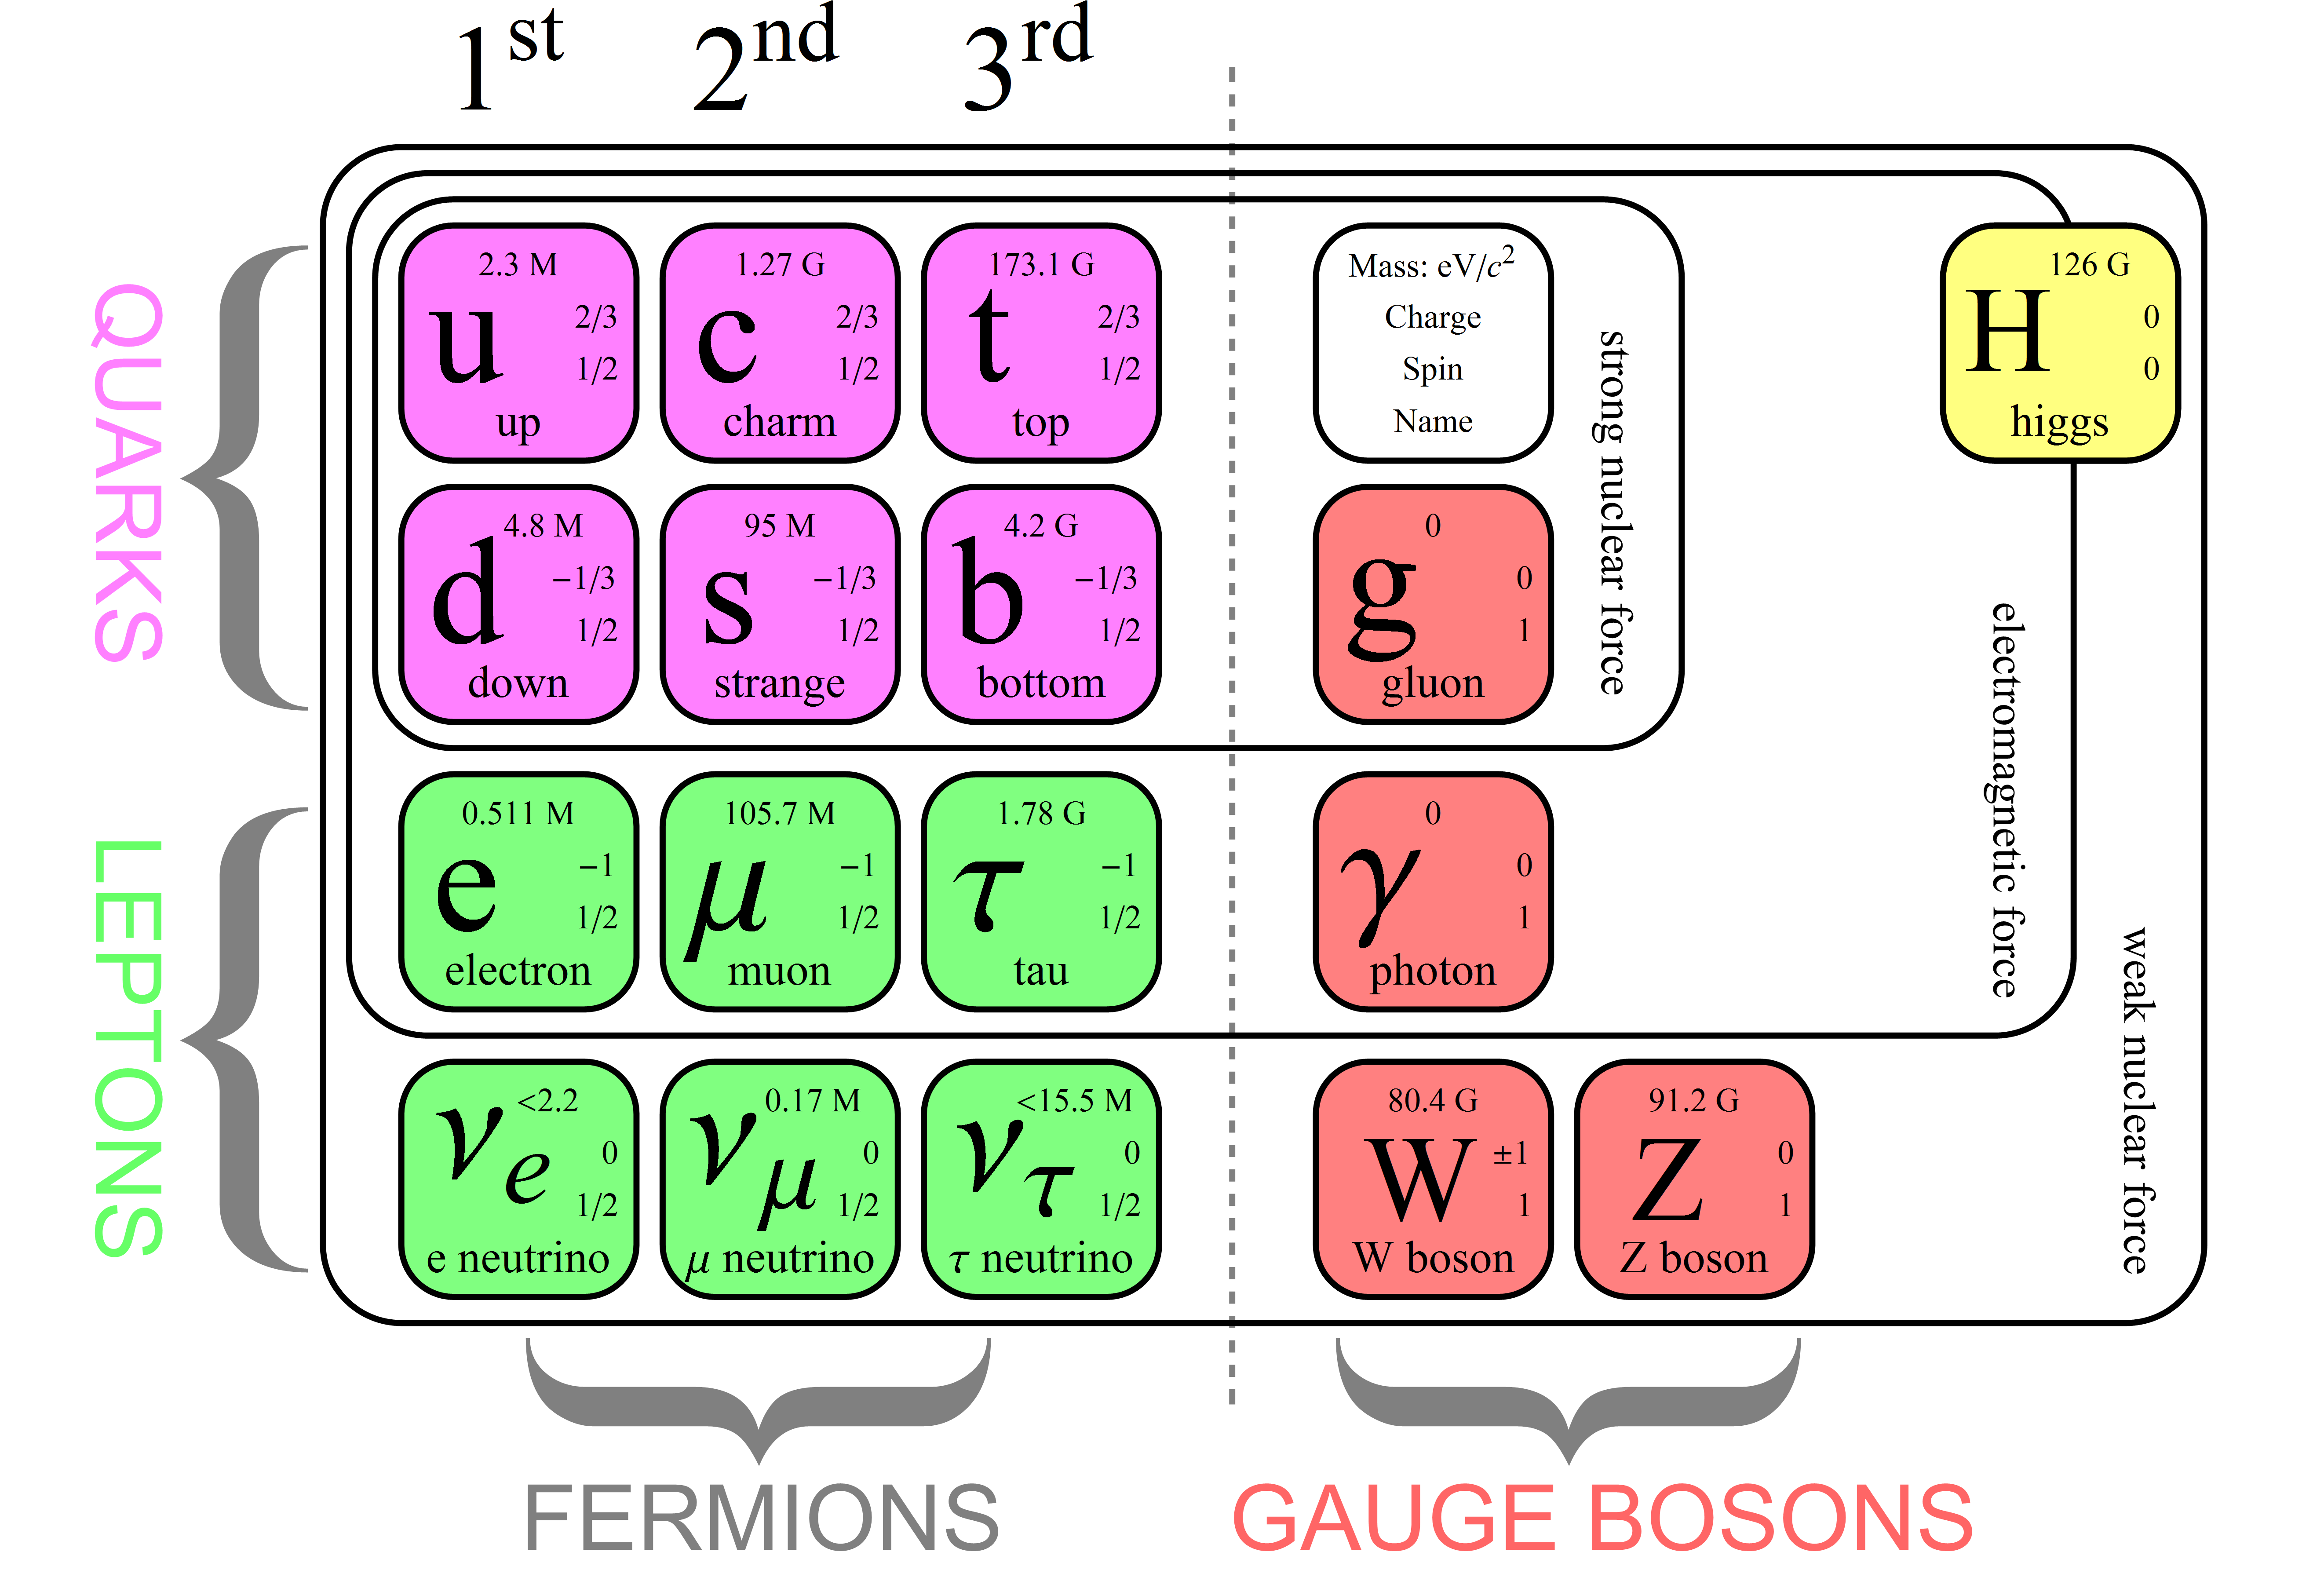
\includegraphics[width=0.9\textwidth]{01StandardModel/figs/particles.png}
  \end{center}
  \vspace{-2mm}
  \caption{Elementary particles described by the SM~\cite{sm-cartoon}.}
  \label{fig:particles}
\end{figure}


All particles are either \emph{fermions} or \emph{bosons}. The fermions (leptons, quarks) have half-integer spin and follow the Fermi-Dirac statistics \cite{Fermi, Dirac}, whereas bosons (gauge bosons, Higgs boson) 
have integer spin and follow the Bose-Einstein statistics \cite{Bose}.

Leptons (spin-$\frac{1}{2}$) include three charged, massive particles (electron $e^-$, muon $\mu^-$ and tau $\tau^-$), which interact via the electromagnetic and weak interactions, and three neutral, (nearly) massless particles, called \emph{neutrinos} ($\nu_{e}$, $\nu_{\mu}$ and $\nu_{\tau}$), which only experience weak interactions.

Six different flavours of quarks (spin-$\frac{1}{2}$) exist: the \emph{up-type} quarks up ($u$), charm ($c$) and  top/truth ($t$), having charge\footnote{Electric charge is always quoted in units of the fundamental charge, defined as minus the charge of the electron.} $+\frac{2}{3}$, and the \emph{down-type} quarks down ($d$), strange ($s$), and bottom/beauty ($b$), which have charge $-\frac{1}{3}$. They can interact via electromagnetic, weak and strong interactions, and they are all massive.

The fundamental interactions are \emph{mediated} by gauge bosons (spin-$1$). The photon ($\gamma$) is responsible for the electromagnetic interaction, whereas the $Z^0$ and $W^\pm$ bosons are the mediators for the weak interaction. These two forces are considered to be different manifestations of a single \emph{electroweak} interaction, which is responsible for all electric and magnetic phenomena as well as some radioactive decays. The strong interaction among quarks is mediated by the gluons $g$. Photon and gluons are massless, whereas the weak force gauge bosons have a non-zero mass.

Each particle has an \emph{antiparticle} partner, which has the same mass as the corresponding particle, but opposite quantum numbers (electric charge, lepton numbers, etc\dots).

Quarks do not exist in a free state: they can only be bound inside \emph{hadrons} via the \emph{confinement} mechanism, a feature of the strong interaction. A hadron can be composed by a quark-antiquark pair (\emph{meson}), or by three quarks or antiquarks (\emph{baryons}). Examples of mesons include the $B^0$ ($\bar b d$) and $D^+$ ($c\bar d$) mesons, whereas the proton ($uud$) and the neutron ($udd$) are examples of baryons. Recently more complex states (tetraquarks~\cite{LHCb-PAPER-2014-014}, pentaquarks~\cite{LHCb-PAPER-2015-029}) have been evidenced.

The non-zero mass of leptons, quarks and weak force gauge bosons would require a gauge symmetry breaking term in the SM Lagrangian density. 
The \emph{Brout-Englert-Higgs mechanism} \cite{BroutEnglert, Higgs, Guralnik} introduces a scalar (spin-$0$) field, called Higgs field, and a potential that allows the Higgs field to have a non-zero vacuum expectation value.
This implies that the gauge symmetry is broken \emph{dynamically}, and that the masses of the particles arise from the resulting interaction with the Higgs field. The quantum of the Higgs field is known as Higgs boson, the last SM particle discovered experimentally \cite{ATLAS, CMS}.

The fourth fundamental interaction, the gravitational force, is described by another field theory, the General Relativity (GR), currently not unified with the SM.

Any experimental signature that is not described by the SM would be a hint for \emph{new physics} (NP). Although the SM is known to be an incomplete theory because of different unsolved problems, such as dark matter, \emph{naturalness}, matter-antimatter asymmetry, lack of SM-GR unification, etc\dots, no evidence for NP has been found so far.

%!TEX root = ../my_thesis.tex
\section{The Cabibbo-Kobayashi-Maskawa matrix}
\label{sec:ckm}

The Lagrangian density describing the weak interactions between quarks and $W^\pm$ (\emph{charged current interaction}) can be written as
\begin{equation}
	\label{eq:Lcc}
	\mathcal L_{cc} = \frac{g}{\sqrt{2}} \left( \begin{array}{ccc} \bar u & \bar c & \bar t \end{array} \right) V_{\rm CKM} \gamma^\mu \frac{\left(1-\gamma^5\right)}{2} \left( \begin{array}{c} d \\ s \\ b \end{array} \right) W^+_{\mu} + h.c.,
\end{equation}
where $g$ is a coupling constant, $\gamma^\mu$ are Dirac matrices and $V_{\rm CKM}$, known as the Cabibbo-Kobayashi-Maskawa (CKM) matrix \cite{PRL-10-1963-531,PTP-49-1973-652}, 
couples the \emph{flavour} eigenstates $d$, $s$ and $b$ to the \emph{mass} (or \emph{physical}) eigenstates $d'$, $s'$ and $b'$:
\begin{equation}
	V_{\rm CKM} = \left( \begin{array}{ccc} V_{ud} & V_{us} & V_{ub} \\ V_{cd} & V_{cs} & V_{cb} \\ V_{td} & V_{ts} & V_{tb} \end{array} \right).  
\end{equation}
The CKM matrix is unitary ($V_{\rm CKM}^\dagger V_{\rm CKM}\equiv 1$), so it can be written in terms of four independent parameters, namely three angles and a \emph{complex phase} $\delta$. 
The latter is the source of all \emph{CP-violating} phenomena in the SM, i.e. asymmetries between particles and antiparticles; in fact, the \emph{complexity} of $V_{\rm CKM}$
implies that the SM Lagrangian density is non \CP-invariant, in agreement with the experimentally observed \CP~violation.

A first, standard parameterisation of the CKM matrix \cite{PRL-53-1984-53} gives
\begin{equation}
	V_{\rm CKM} = \left( \begin{array}{ccc} c_{12}c_{13} & s_{12}c_{13} & s_{13}e^{-i\delta} \\ 
								-s_{12}c_{23}-c_{12}s_{23}s_{13}e^{i\delta} &  c_{12}c_{23}-s_{12}s_{23}s_{13}e^{i\delta} & s_{23}c_{13} \\
								s_{12}s_{23}-c_{12}c_{23}s_{13}e^{i\delta} &  -c_{12}s_{23}-s_{12}c_{23}s_{13}e^{i\delta} & c_{23}c_{13} \end{array} \right),
\end{equation}
where $s_{ij}=\sin\theta_{ij}$ and $c_{ij}=\cos\theta_{ij}$.

Another, useful parameterisation is given by \emph{Wolfenstein} \cite{PRL-51-1983-1945} and points out the order of magnitude of each matrix element. By defining the quantities $\lambda$, $A$, $\rho$ and $\eta$ with
\begin{align}
	s_{12} &= \lambda = \frac{|V_{us}|}{\sqrt{|V_{ud}|^2+|V_{us}|^2}}, & s_{23} &= A\lambda^2=A\left|\frac{V_{cb}}{V_{us}}\right|, \\
	s_{13}e^{i\delta} &= V^{*}_{ub} = A\lambda^3(\rho+i\eta), 
\end{align}
the $V_{\rm CKM}$ matrix can be rewritten as a series expansion in powers of $\lambda$, given that $\lambda$ is a small number:
\begin{equation}
	\label{eq:ckm}
	V_{\rm CKM} = \left( \begin{array}{ccc} 1-\lambda^2/2 & \lambda & A\lambda^3(\rho-i\eta) \\ 
									-\lambda & 1-\lambda^2/2 & A\lambda^2 \\
									A\lambda^3(1-\rho-i\eta) & -A\lambda^2 & 1 \end{array} \right) + \mathcal O(\lambda^4).
\end{equation}
From Eq.~\ref{eq:ckm}, one can see that quark transitions within the same family (\eg $u\to d$) are more probable, whereas transitions between different families (\eg $b\to c$) are more suppressed. \CP~violation is a consequence of $\eta\neq0$ and $\eta\neq\pi$.

The unitarity condition $V_{\rm CKM}^\dagger V_{\rm CKM}\equiv 1$ can be rewritten in terms of six scalar equations. Two of them are particularly relevant for the $b$-hadron phenomenology:
\begin{align}
	\label{eq:ut}
	V_{ud}V_{ub}^* + V_{cd}V_{cb}^* + V_{td}V_{tb}^* &= 0, \\
	\label{eq:ut_s}
	V_{us}V_{ub}^* + V_{cs}V_{cb}^* + V_{ts}V_{tb}^* &= 0.
\end{align}
These two equations can be graphically represented as \emph{triangles} is the $(\bar\rho, \bar\eta)$ complex plane,
where $\bar\rho$ and $\bar\eta$ are defined in terms of the series expansions 
$\bar\rho=\rho(1-\lambda^2/2+\dots)$ and $\bar\eta=\eta(1-\lambda^2/2+\dots)$, respectively. 
Having introduced the following angles,
\begin{align}
	\label{eq:alpha_beta}
	\alpha &= \phi_2 = \arg\left[-\frac{V_{td}V_{tb}^*}{V_{ud}V_{ub}^*}\right], & \beta &= \phi_1 = \arg\left[-\frac{V_{cd}V_{cb}^*}{V_{td}V_{tb}^*}\right], \\
	\gamma &= \phi_3 = \arg\left[-\frac{V_{ud}V_{ub}^*}{V_{cd}V_{cb}^*}\right], & \beta_s &= \chi = \arg\left[-\frac{V_{cb}V_{cs}^*}{V_{tb}V_{ts}^*}\right],
\end{align}
the triangles given by Eqs.~\ref{eq:ut} and~\ref{eq:ut_s} can be depicted as shown in Fig.~\ref{fig:ut}. The first triangle, defined by Eq.~\ref{eq:ut}, is known as the \emph{Unitarity Triangle} (UT) and its elements can be
measured from analyses of $B^0$, $B^0_s$ and $B^{\pm}$ decays. The other triangle (Eq.~\ref{eq:ut_s}) can be studied from decays of $B^0_s$ mesons.

The amount of \CP~violation in the SM is given by the Jarlskog invariant $J$~\cite{Jarlskog:1985ht}, which satisfies
\begin{equation}
  \Im\left[V_{ij}V_{kl}V^{*}_{il}V^{*}_{kj}\right] = J \sum\limits_{m,n}\varepsilon_{ikm}\varepsilon_{jln}\,,
\end{equation}
where $\varepsilon$ denotes the fully-antisymmetric tensor. The value of $J$ is too small by several orders of magnitude to explain the observed matter-antimatter asymmetry in the universe, according to the baryogenesis model~\cite{Sakharov:1967dj}. So, new sources of \CP~violation not foreseen by the SM have to exist, and thus measuring the UT with the highest possible precision is crucial to constrain these new physics scenarios.

\begin{figure}[htbp]
  \begin{center}
    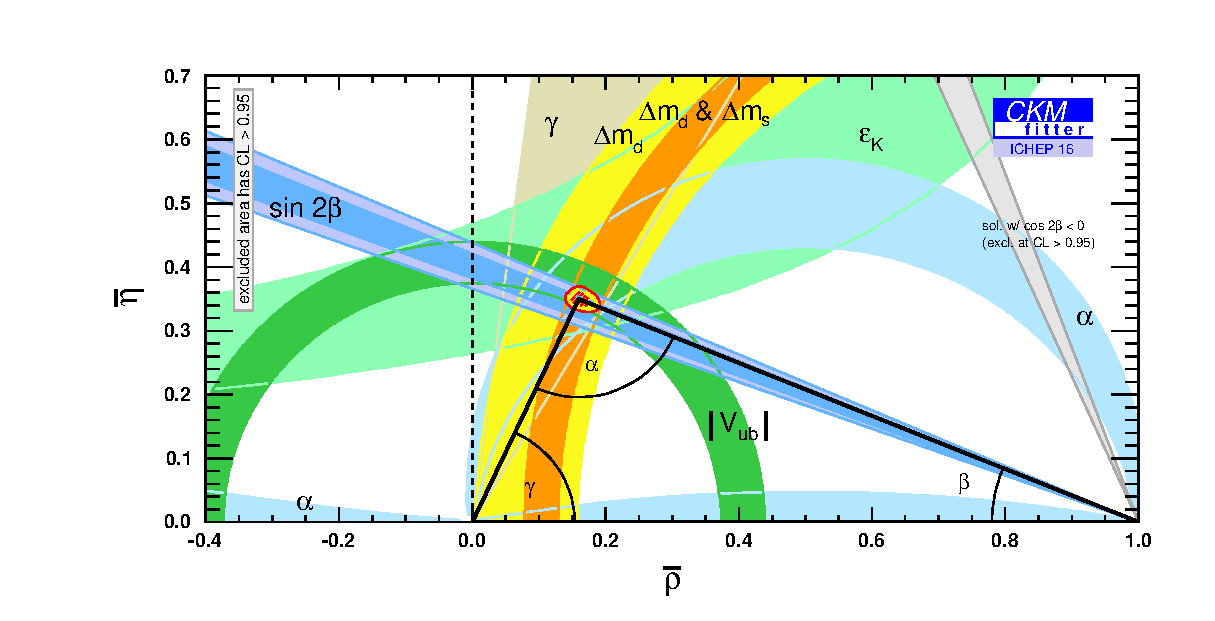
\includegraphics[width=0.9\textwidth]{02CKM/figs/ut.eps} \\
    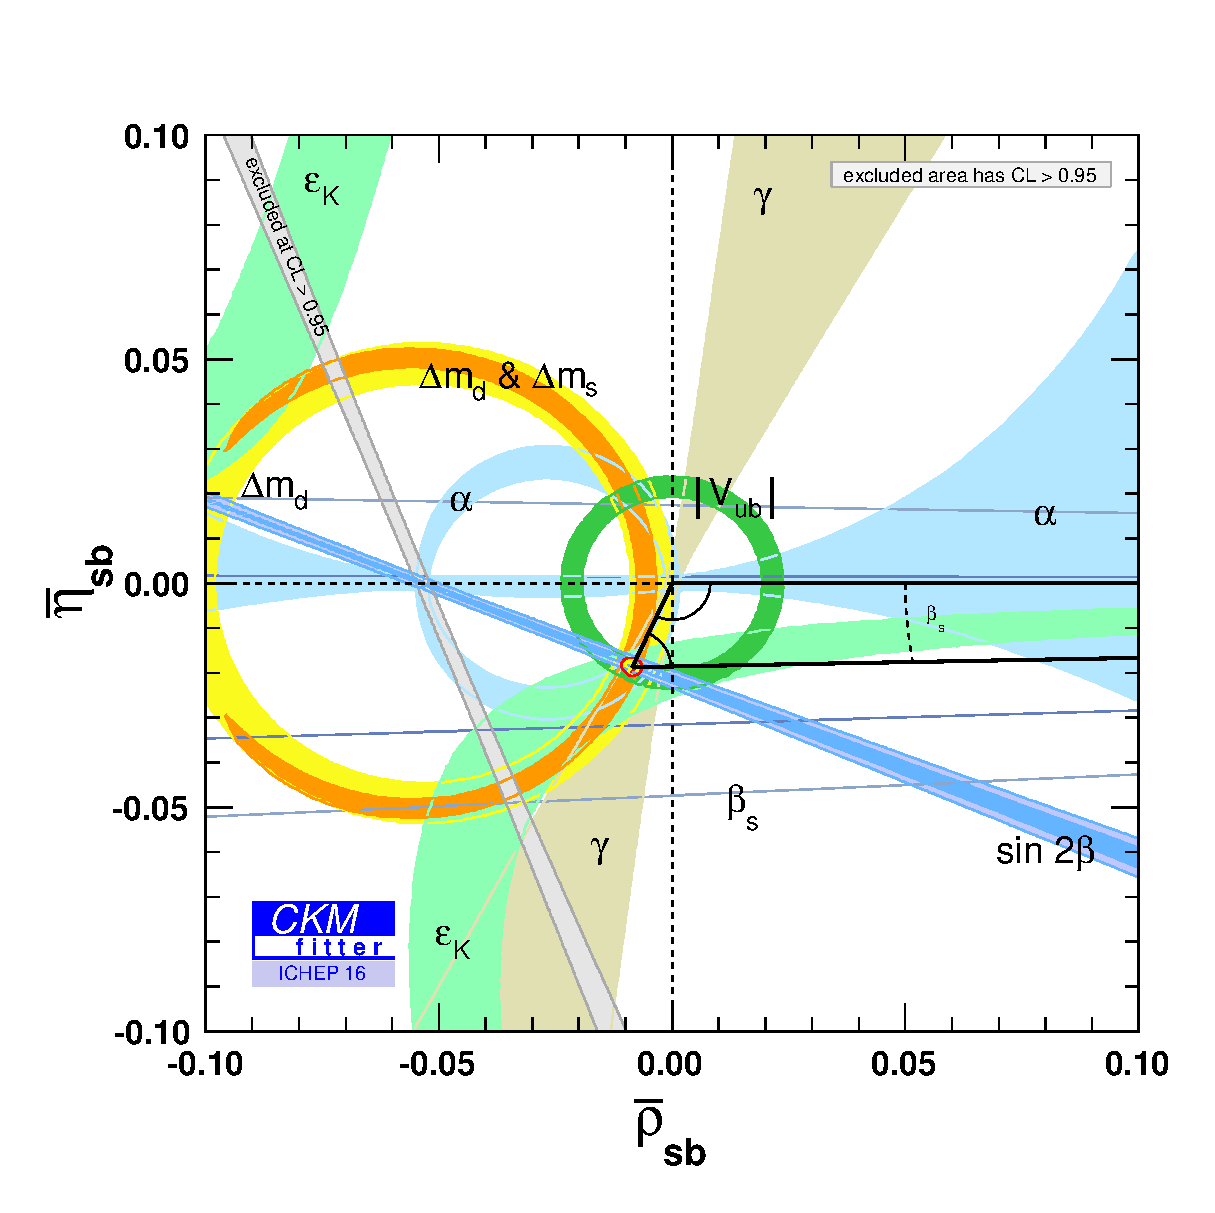
\includegraphics[width=0.9\textwidth]{02CKM/figs/ut_s.eps} \\
  \end{center}
  \vspace{-2mm}
  \caption{Graphical representation of two of the six unitarity conditions of the CKM matrix, superimposed with the current experimental constraints~\cite{CKMfitter2015}.}
  \label{fig:ut}
\end{figure}

%!TEX root = ../my_thesis.tex
\section[Physics of the neutral $B$ mesons]{Physics of the neutral \boldmath{$B$} mesons}
\label{sec:Bphysics}

The theory of neutral $B$ meson oscillation, decays and \CP~violation presented here is derived from Refs.~\cite{PDG,CPviolation}.

\subsection{Oscillation of neutral mesons}

Neutral $B$ meson states are characterised by the following quark content:
\begin{align}
	\ket{B^0} &= \ket{d\bar b}, & \ket{\bar B^0} &= \ket{\bar d b}, \\
	\ket{B_s^0} &= \ket{s\bar b}, & \ket{\bar B_s^0} &= \ket{\bar s b}. 
\end{align}
All neutral mesons will be denoted as $P^0$ or $\bar P^0$ hereafter. The $\bar P^0$ state is obtained from $P^0$
via the \CP~operator up to an arbitrary phase factor $e^{i\phi_{CP}}$.
Since charged currents do not conserve flavour quantum numbers (e.g. strangeness, beauty etc\dots),
a neutral meson can transform itself into its own anti-meson, and vice versa. 
So, the time evolution of a neutral $B$ meson system can be generally written as
\begin{equation}
	\ket{\Psi(t)} = a(t)\ket{P^0} + b(t)\ket{\bar P^0} + \sum_i c_i(t) \ket{f_i},
\end{equation}
where $\ket{f_i}$ are all the possible final states with $c_i(0)=0$ as initial condition.

Since the typical timescale of weak interactions is much longer than the strong interaction timescale,
we can neglect all weak interactions among final states (\emph{Weisskopf-Wigner approximation}). 
So, we can write the Schroedinger equation for $\ket{\Psi(t)}$ in terms of an effective, non-hermitian 
hamiltonian $\mathcal H$:
\begin{equation}
	\label{eq:schroedinger}
	i\partial_t \left( \begin{array}{c} a(t) \\ b(t) \end{array} \right) = \mathcal H \left( \begin{array}{c} a(t) \\ b(t) \end{array} \right) = 
	\left( \begin{array}{cc} H_{11} & H_{12} \\ H_{21} & H_{22} \end{array} \right) \left( \begin{array}{c} a(t) \\ b(t) \end{array} \right). 
\end{equation} 
The $\mathcal H$ matrix can be rewritten as the sum of two hermitian matrices $M$ and $\Gamma$:
\begin{equation}
	\label{eq:effhamiltonian}
	\mathcal H = M - \frac{i}{2} \Gamma = 
	\left( \begin{array}{cc} M_{11} & M_{12} \\ M_{21} & M_{22} \end{array} \right) - \frac{i}{2} \left( \begin{array}{cc} \Gamma_{11} & \Gamma_{12} \\ \Gamma_{21} & \Gamma_{22} \end{array} \right).
\end{equation}
Assuming $CPT$~invariance ($H_{11}=H_{22}=H_0$, $M_{11}=M_{22}=M_0$, $\Gamma_{11}=\Gamma_{22}=\Gamma_0$), the eigenvalues of $\mathcal H$ are
\begin{align}
	\lambda_{L} &= m_{L} - \frac{i}{2}\Gamma_{L} = H_0 + \sqrt{H_{12}H_{21}} = H_0 + \sqrt{\left(M_{12}-\frac{i}{2}\Gamma_{12}\right)\left(M_{12}^*-\frac{i}{2}\Gamma_{12}^*\right)}, \\
	\lambda_{H} &= m_{H} - \frac{i}{2}\Gamma_{H} = H_0 - \sqrt{H_{12}H_{21}} = H_0 - \sqrt{\left(M_{12}-\frac{i}{2}\Gamma_{12}\right)\left(M_{12}^*-\frac{i}{2}\Gamma_{12}^*\right)},
\end{align}
where $L$ (``light'') and $H$ (``heavy'') refer to the value of the mass for each eigenstate.
The corresponding eigenvectors are
\begin{align}
	\label{eq:eigenvectors}
	\ket{P_L} &= p\ket{P^0} + q\ket{\bar P^0}, & \ket{P_H} &= p\ket{P^0} - q\ket{\bar P^0},	
\end{align}
where $p$ and $q$ satisfy $|p|^2+|q|^2 = 1$ and are given by
\begin{equation}
	\frac{q}{p} = \sqrt{ \frac{H_{21}}{H_{12}} } = 
			\sqrt{ \frac{M_{21}-\frac{i}{2}\Gamma_{21}}{M_{12}-\frac{i}{2}\Gamma_{12}} } =
			 \sqrt{ \frac{M^*_{12}-\frac{i}{2}\Gamma^*_{12}}{M^*_{21}-\frac{i}{2}\Gamma^*_{21}} }.  
\end{equation}
The relative phase $\phi_M$ between $M_{12}$ and $\Gamma_{12}$ is an observable quantity describing indirect \CP~violation (Sec.~\ref{sec:cpv}):
\begin{align}
	M_{12} &= M_{12}^*e^{i\phi_{CP}}, & \Gamma_{12} &= \Gamma_{12}^*e^{i\phi_{CP}}e^{i\phi_M}.
\end{align}
For the neutral $B$ meson system, the ratio $|\Gamma_{12}/M_{12}|$ is expected to be small in the SM; as a consequence, it can be shown that
\begin{equation}
	\label{eq:pqratio}
	\frac{q}{p} = -e^{-i\phi_M} \left[1-\frac{1}{2}\left|\frac{\Gamma_{12}}{M_{12}}\right|\sin\phi_M + \mathcal O\left( \left|\frac{\Gamma_{12}}{M_{12}}\right|^2 \right) \right],
\end{equation}
which implies $|q/p|\sim1$.

The difference and the average of the masses and widths of the two mass eigenstates are defined as
\begin{align}
	\label{eq:deltaM}
	\Delta m &= m_H - m_L = \Re(\lambda_H - \lambda_L), & m &= \frac{m_L+m_H}{2} = \frac{\Re(\lambda_H + \lambda_L)}{2}, \\
	\label{eq:deltaGamma}
	\Delta\Gamma &= \Gamma_L - \Gamma_H = -2\Im(\lambda_L - \lambda_H), & \Gamma &= \frac{\Gamma_L+\Gamma_H}{2} = -\frac{\Re(\lambda_H + \lambda_L)}{4}. 
\end{align}
The sign convention for $\Delta\Gamma$ is chosen to have a positive experimental value for the $B^0_s$ system (for $B^0$, experiments give a result compatible with zero, in agreement with the SM).

The time evolution of the states $\ket{P^0(t)}$ and $\ket{\bar P^0(t)}$ when they are initially produced as $\ket{P^0(0)}$ and $\ket{\bar P^0(0)}$ can be obtained from the effective hamiltonian:
\begin{align}
	\ket{P^0(t)} &= g_+(t) \ket{P^0(t)} + \frac{q}{p} g_-(t) \ket{\bar P^0(t)}, \\
	\ket{\bar P^0(t)} &= g_+(t) \ket{\bar P^0(t)} + \frac{p}{q} g_-(t) \ket{P^0(t)}.
\end{align}
The functions $g_{\pm}(t)$ are built in terms of the eigenvalues:
\begin{equation}
	g_{\pm}(t) = \frac{1}{2} \left( e^{-im_H t-\frac{1}{2}\Gamma_H t} \pm e^{-im_L t-\frac{1}{2}\Gamma_L t} \right).
\end{equation}
The probabilities that a state initially produced as $P^0$ or $\bar P^0$  becomes a $P^0$ or $\bar P^0$ at~time~$t$~are
\begin{align}
	\left| \braket{P^0(0) | P^0(t) } \right|^2 &= |g_+(t)|^2 = \frac{e^{-\Gamma t}}{2} \left( \cosh\frac{\Delta\Gamma t}{2} + \cos\Delta m t \right), \\
	\label{eq:P0barToP0}
	\left| \braket{\bar P^0(0) | P^0(t) } \right|^2 &= \left| \frac{q}{p} \right|^2 |g_-(t)|^2 = \left| \frac{q}{p} \right|^2 \frac{e^{-\Gamma t}}{2} \left( \cosh\frac{\Delta\Gamma t}{2} - \cos\Delta m t \right), \\
	\label{eq:P0ToP0bar}
	\left| \braket{P^0(0) | \bar P^0(t) } \right|^2 &= \left| \frac{p}{q} \right|^2 |g_-(t)|^2 = \left| \frac{p}{q} \right|^2 \frac{e^{-\Gamma t}}{2} \left( \cosh\frac{\Delta\Gamma t}{2} - \cos\Delta m t \right), \\
	\left| \braket{\bar P^0(0) | \bar P^0(t) } \right|^2 &= |g_+(t)|^2 = \frac{e^{-\Gamma t}}{2} \left( \cosh\frac{\Delta\Gamma t}{2} + \cos\Delta m t \right).
\end{align}
The equations above describe the \emph{oscillation} of the $B^0$ and $B^0_s$ mesons.

\subsection{Decay of neutral mesons}
\label{sec:neutral_meson_decays}

The amplitude for the decay of a neutral meson into a final state $f$ can be obtained from the effective hamiltonian $\mathcal H$:
\begin{align}
	A_f &= \bra{f}\mathcal H \ket{P^0}, & \bar A_f &= \bra{f}\mathcal H \ket{\bar P^0}, \\
	A_{\bar f} &= \bra{\bar f}\mathcal H \ket{P^0}, & \bar A_{\bar f} &= \bra{\bar f}\mathcal H \ket{\bar P^0}.
\end{align}
After defining the parameters
\begin{align}
	\lambda_f &= \frac{q}{p}\frac{\bar A_f}{A_f}, & \frac{1}{\bar\lambda_{\bar f}} &= \lambda_{\bar f} = \frac{q}{p}\frac{\bar A_{\bar f}}{A_{\bar f}},
\end{align}
it is possible to write the \emph{decay rates} for neutral mesons decaying into $f$ or $\bar f$: 
\begin{equation}
	\label{eq:P0tof}
	\begin{split}
		\frac{d\Gamma(P^0\to f)}{dt}(t) &= N_f |A_f|^2 \frac{1+|\lambda_f|^2}{2}e^{-\Gamma t} \\
		& \left[ \cosh\left(\frac{\Delta\Gamma t}{2}\right) + D_f \sinh\left(\frac{\Delta\Gamma t}{2}\right) + C_f \cos \left( \Delta m t \right) - S_f \sin \left( \Delta m t \right) \right],   
	\end{split}
\end{equation}
\begin{equation}
	\label{eq:P0bartof}
	\begin{split}
		\frac{d\Gamma(\bar P^0\to f)}{dt}(t) &= N_f |A_f|^2 \left|\frac{p}{q}\right|^2 \frac{1+|\lambda_f|^2}{2}e^{-\Gamma t} \\
		& \left[ \cosh\left(\frac{\Delta\Gamma t}{2}\right) + D_f \sinh\left(\frac{\Delta\Gamma t}{2}\right) - C_f \cos \left( \Delta m t \right) + S_f \sin \left( \Delta m t \right) \right],   
	\end{split}
\end{equation}
\begin{equation}
	\label{eq:P0tofbar}
	\begin{split}
		\frac{d\Gamma(P^0\to \bar f)}{dt}(t) &= N_f |\bar A_{\bar f}|^2 \left|\frac{q}{p}\right|^2 \frac{1+|\bar \lambda_{\bar f}|^2}{2}e^{-\Gamma t} \\
		& \left[ \cosh\left(\frac{\Delta\Gamma t}{2}\right) + D_{\bar f} \sinh\left(\frac{\Delta\Gamma t}{2}\right) + C_{\bar f} \cos \left( \Delta m t \right) - S_{\bar f} \sin \left( \Delta m t \right) \right],   
	\end{split}
\end{equation}
\begin{equation}
	\label{eq:P0bartofbar}
	\begin{split}
		\frac{d\Gamma(\bar P^0\to \bar f)}{dt}(t) &= N_f |\bar A_{\bar f}|^2 \frac{1+|\bar \lambda_{\bar f}|^2}{2}e^{-\Gamma t} \\
		& \left[ \cosh\left(\frac{\Delta\Gamma t}{2}\right) + D_{\bar f} \sinh\left(\frac{\Delta\Gamma t}{2}\right) - C_{\bar f} \cos \left( \Delta m t \right) + S_{\bar f} \sin \left( \Delta m t \right) \right],
	\end{split}
\end{equation}
where $N_f$ is a time-independent normalisation factor and
\begin{align}
	\label{eq:cp_f}
	D_f &= -\frac{2\Re \lambda_f}{1+|\lambda_f|^2}, & C_f &= \frac{1-|\lambda_f|^2}{1+|\lambda_f|^2}, & S_f &= \frac{2\Im \lambda_f}{1+|\lambda_f|^2}, \\
	\label{eq:cp_fbar}	
	D_{\bar f} &= -\frac{2\Re \bar\lambda_{\bar f}}{1+|\bar\lambda_{\bar f}|^2}, & C_{\bar f} &= -\frac{1-|\bar\lambda_{\bar f}|^2}{1+|\bar\lambda_{\bar f}|^2}, & S_{\bar f} &= -\frac{2\Im \bar\lambda_{\bar f}}{1+|\bar\lambda_{\bar f}|^2}
\end{align}
are known as \emph{\CP~coefficients}.

\subsection[$CP$~violation in neutral meson systems]{\boldmath{$CP$}~violation in neutral meson systems}
\label{sec:cpv}

Three types of \CP~violation can occur. They are briefly sketched in Fig.~\ref{fig:CPVclasses} and described in the following paragraphs.

\begin{figure}[htbp]
  \begin{center}
    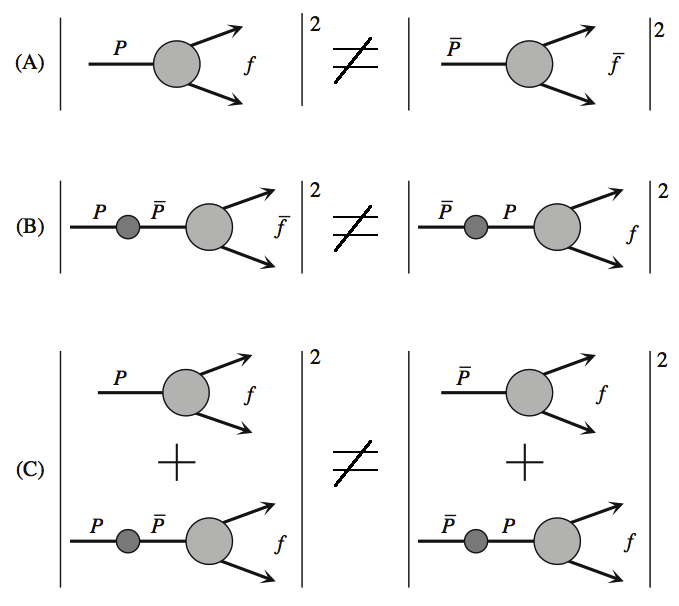
\includegraphics[width=0.9\textwidth]{03BPhysics/figs/CPVclasses.png} \\
  \end{center}
  \vspace{-2mm}
  \caption{Graphical representation of \CP~violation in decay (A), mixing (B) and interference between mixing and decay (C)~\cite{CPviolation}.}
  \label{fig:CPVclasses}
\end{figure}

\subsubsection*{\boldmath{$CP$}~violation in decays} 

\CP~violation in decays, also known as \emph{direct} \CP~violation, happens when the decay rate for $P \to f$ is different from that of the \CP-conjugated process $\bar P \to \bar f$:
\begin{equation}
	\left| \frac{\bar A_{\bar f}}{A_{f}} \right| \neq 1.
\end{equation}
This kind of \CP~violation occurs if, for each decay, at least two amplitudes with different weak ($\phi_j$) and strong ($\delta_j$) phases contribute:
\begin{align}
	A_f &= \sum_j |A_j| e^{i(\delta_j + \phi_j)}, & \bar A_{\bar f} &= \sum_j  |\bar A_j| e^{i(\delta_j - \phi_j)}.
\end{align}
In fact, the strong phases are invariant under \CP~conjugation, whereas the weak phases change sign. 
The following asymmetry between final states can be measured to determine direct \CP~violation experimentally for \emph{charged mesons}, where mixing effects are absent:
\begin{equation}
	\mathcal A_{f^{\pm}} = \frac{\Gamma(P^-\to f^-) - \Gamma(P^+\to f^+) }{\Gamma(P^-\to f^-) + \Gamma(P^+\to f^+)} = \frac{\left| \frac{\bar A_{\bar f}}{A_{f}} \right|^2-1}{\left| \frac{\bar A_{\bar f}}{A_{f}} \right|^2+1}
\end{equation}

\subsubsection*{\boldmath{$CP$}~violation in mixing}

\CP~violation in mixing, also called \emph{indirect} \CP~violation, occurs when the oscillation rate for $\bar P^0\to P^0$ is different from that of the \CP-conjugated process $P^0\to \bar P^0$.
These two oscillation probabilities are given by Eqs.~\ref{eq:P0barToP0} and~\ref{eq:P0ToP0bar}. It turns out that they are identical unless
\begin{equation}
	\left| \frac{q}{p} \right| \neq 1.
\end{equation}
From Eq.~\ref{eq:pqratio}, it can be seen that \CP~violation in mixing occurs when the relative phase $\phi_M$ is different from any multiple of $\pi$. It is possible to measure the $|q/p|$ ratio by comparing the oscillation rates in flavour-specific, semileptonic decays of neutral mesons $P^0\to l^+ X$ and $\bar P^0\to l^-X$, where no direct \CP~violation occurs. The decays where oscillation occurred are identified by reconstructing ``wrong sign'' leptons.
The so-called semileptonic asymmetry
\begin{equation}
	\mathcal A_{\rm SL} = \frac{\frac{d\Gamma(\bar P^0\to l^+X)}{dt} - \frac{d\Gamma(P^0\to l^-X)}{dt} }{\frac{d\Gamma(\bar P^0\to l^+X)}{dt} + \frac{d\Gamma(P^0\to l^-X)}{dt}} = \frac{1-|q/p|^4}{1+|q/p|^4}
\end{equation} 
is independent of time.

\subsubsection*{\boldmath{$CP$}~violation in the interference between mixing and decay}

This type of decay occurs when a neutral meson can decay directly to a given final state, $P^0\to f$, or via mixing, $P^0\to \bar P^0 \to f$. 
This can happen only if the final state $f$ is common to both $P^0$ and $\bar P^0$.
This type of \CP~violation can occur also if other sources of \CP~violation (mixing or decay) are absent.
In general, the interference between mixing and decay can be accessed by studying the following asymmetries:
\begin{align}
	\label{eq:asymmetry_f}
	\mathcal A_f(t) &= \frac{ \frac{d\Gamma(P^0\to f)}{dt} - \frac{d\Gamma(\bar P^0\to f)}{dt} }{ \frac{d\Gamma(P^0\to f)}{dt} + \frac{d\Gamma(\bar P^0\to f)}{dt}}, &
	\mathcal A_{\bar f}(t) &= \frac{ \frac{d\Gamma(P^0\to \bar f)}{dt} - \frac{d\Gamma(\bar P^0\to \bar f)}{dt} }{ \frac{d\Gamma(P^0\to \bar f)}{dt} + \frac{d\Gamma(\bar P^0\to \bar f)}{dt}}.
\end{align}
A relevant example is the case of neutral $B$ mesons, where $|q/p|=1$. Using Eqs.~\ref{eq:P0tof}--\ref{eq:P0bartofbar}, the asymmetries of Eq.~\ref{eq:asymmetry_f} take the following forms:
\begin{align}
	\mathcal A_f(t) &= \frac{C_f \cos(\Delta m t) - S_f \sin(\Delta m t)}{\cosh\left(\frac{\Delta\Gamma t}{2}\right) + D_f \sinh\left(\frac{\Delta\Gamma t}{2}\right)}, &
	\mathcal A_{\bar f}(t) &= \frac{-C_{\bar f} \cos(\Delta m t) + S_{\bar f} \sin(\Delta m t)}{\cosh\left(\frac{\Delta\Gamma t}{2}\right) + D_{\bar f} \sinh\left(\frac{\Delta\Gamma t}{2}\right)}.
\end{align}
The \CP~coefficients can be directly measured from a time-dependent analysis of certain $B$ decays. 

%!TEX root = ../my_thesis.tex

\section[$\Bz\to\Dmp\pipm$ analysis motivation and phenomenology]{\boldmath{$\Bz\to\Dpm\pimp$} analysis motivation and phenomenology}
\label{sec:intro}
\setlength{\textfloatsep}{30pt}
\begin{figure}[t]
        \begin{center}
                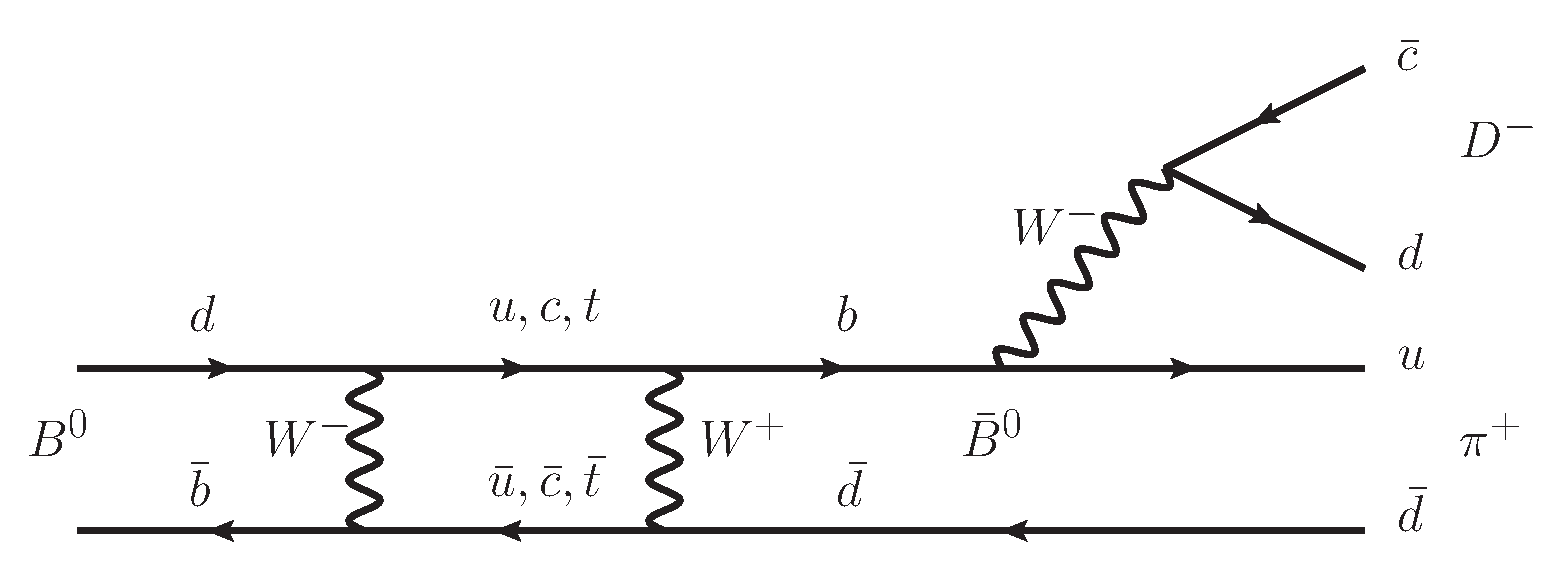
\includegraphics[width=0.8\linewidth]{01Introduction/figs/Mixed.eps}
                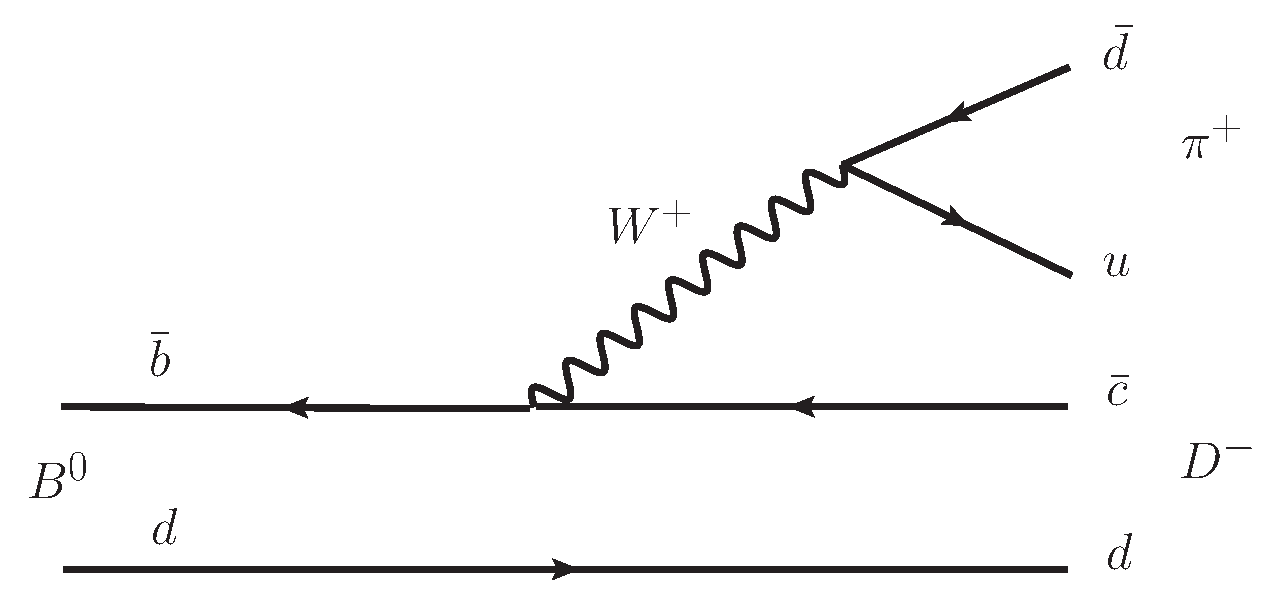
\includegraphics[width=0.7\linewidth]{01Introduction/figs/Unmixed.eps}
                %\vspace*{-1.0cm}                                                                                                           
        \end{center}
        \vspace{-2mm}
        \caption{Feynman diagrams contributing to $\Bz\to \Dm\pip$, with (top) and without (bottom) mixing.}
        \label{fig:Feynman}
        \afterpage{\global\setlength{\textfloatsep}{\oldtextfloatsep}}
\end{figure}
In this thesis, a decay-time dependent analysis of the decay $\Bz\to
\Dmp\pipm$ is presented, where the $\Dpm$ meson is reconstructed as $\Dpm\to\Kmp\pipm\pipm$. The 
pion produced together with the $\Dpm$ meson will be named \emph{bachelor} or \emph{companion} hereafter.
The objective of this study is to perform a
measurement of \CP~asymmetries, in order to constrain the CKM angle
$\gamma$~\cite{PRL-10-1963-531,PTP-49-1973-652}. The $\gamma$ angle is particularly important to test 
the CKM picture of the \CP~violation. In fact, $\gamma$ is the least-known parameter of the UT, whereas 
the theoretical predictions for its value are very clean and free from hadronic uncertainties~\cite{Fleischer:2003yb,Aleksan:1991nh,Dunietz:1987bvsss}. 
So, improving the experimental precision on $\gamma$ is a milestone of the current Flavour Physics programme.
\CP~violation appears in the interference between the Cabibbo favoured $b\to c$
amplitude without mixing, $A(\Bz\to \Dm\pip)$, and the Cabibbo suppressed $b\to u$
amplitude with mixing, $A(\Bz\to\Bzb\to\Dm\pip)$. Two of the corresponding
Feynman diagrams for these amplitudes are depicted in Fig.~\ref{fig:Feynman}.

The measurement is performed by analysing the four time-dependent decay
rates \\
$\frac{d\Gamma(\Bz\to\Dm\pip)}{dt}$, $\frac{d\Gamma(\Bz\to\Dp\pim)}{dt}$, $\frac{d\Gamma(\Bzb\to\Dm\pip)}{dt}$ and $\frac{d\Gamma(\Bzb\to \Dp\pim)}{dt}$. 
Identifying the final state as $f=\Dm\pip$ or $\bar f=\Dp\pim$, and assuming $CPT$ symmetry, no \CP~violation in mixing ($|q/p|=1$) and decay
($|A_f|^2=|\bar A_{\bar f}|^2$, $|A_{\bar f}|^2=|\bar A_f|^2$), and $\Delta\Gamma=0$, the time-dependent decay rates for $B$ mesons initially
produced as $\Bz$ or $\Bzb$ can be written as
\begin{align}
	\frac{d\Gamma(\Bz\to f)}{dt}(t) &= \frac{1}{4\tau} e^{-t/\tau} \left[ 1 + C_{f} \cos\left(\Delta m t\right) - S_{f} \sin\left(\Delta m t\right) \right], \label{eq:decay-rate-Bf}\\
	\frac{d\Gamma(\Bzb\to f)}{dt}(t) &= \frac{1}{4\tau} e^{-t/\tau} \left[ 1 - C_{f} \cos\left(\Delta m t\right) + S_{f} \sin\left(\Delta m t\right) \right],\\
	\frac{d\Gamma(\Bz\to \bar f)}{dt}(t) &= \frac{1}{4\tau} e^{-t/\tau} \left[ 1 + C_{\bar f} \cos\left(\Delta m t\right) - S_{\bar f} \sin\left(\Delta m t\right) \right],\\
	\frac{d\Gamma(\Bzb\to \bar f)}{dt}(t) &= \frac{1}{4\tau} e^{-t/\tau} \left[ 1 - C_{\bar f} \cos\left(\Delta m t\right) + S_{\bar f} \sin\left(\Delta m t\right) \right], \label{eq:decay-rate-Bbfb}
\end{align}
where $\Delta m$ and $\tau=1/\Gamma$ are given by Eqs.~\ref{eq:deltaM} and~\ref{eq:deltaGamma}, respectively.
The \CP~coefficients defined in Eqs.~\ref{eq:cp_f} and~\ref{eq:cp_fbar}, can be expressed as
\begin{align}
	S_{f}&=-\frac{2r_{D\pi}\sin[\delta-(\gamma+2\beta)]}{1+r_{D\pi}^{2}}, & S_{\bar f}&=\frac{2r_{D\pi}\sin[\delta+(\gamma+2\beta)]}{1+r_{D\pi}^{2}}, \\
	C_{f}&=-C_{\bar f}=C=\frac{1-r_{D\pi}^{2}}{1+r_{D\pi}^{2}},
\end{align}
where $\beta$ (Eq.~\ref{eq:alpha_beta}) is related to the $\Bz$ mixing
phase, 
\begin{equation}
  r_{D\pi} = \frac{|\bar A_f|}{|A_f|} = \frac{|A_{\bar f}|}{|\bar A_{\bar f}|}
\end{equation}
is the magnitude of
the ratio between the doubly Cabibbo suppressed and favoured amplitudes, and
$\delta$ is the strong phase difference between these amplitudes.

A measurement of $\gamma$ can be obtained by measuring the \CP~coefficients and
taking external measurements of $\beta$ and $r_{D\pi}$ as input. The angle $\beta$ is
known with very high precision, both theoretically and
experimentally~\cite{LHCb-PAPER-2015-005}. An estimation of $r_{D\pi}$ was performed by the
BaBar and Belle collaborations~\cite{Aubert:2008zi,Das:2010be}, by measuring the
branching fraction of $\Bz\to D_{s}^{(*)+} \pim$ decays and assuming SU(3)
symmetry, yielding an average of about $1.7\%$ with a relative error around
15\%, mainly due to SU(3) symmetry breaking. Because of the very small value of $r_{D\pi}$, 
this analysis is not sensitive to $C_{f}$ and $C_{\bar f}$; for this reason, 
these coefficients are simply fixed to $+1$ and $-1$, respectively.

The small value for the $r_{D\pi}$ parameter, which reduces the sensitivity on $S_{f/\bar f}$, makes this measurement challenging 
as compared to similar analyses like $\Bs\to\Dsmp\Kpm$. 
However, the $\Bs$ production rate is significantly smaller 
than the $\Bz$ production fraction ($f_s/f_d=0.259\pm0.015$~\cite{LHCb:2013lka}). 
Moreover, the $\Bs\to\Dsmp\Kpm$ branching ratio, $(2.27\pm0.19)\times 10^{-4}$~\cite{Louvot:2008sc}, is much smaller than 
the $\Bz\to\Dm\pip$ branching ratio, $(2.52\pm0.13)\times 10^{-3}$~\cite{PDG2017}.  
So, the resulting, larger number of $\Bz\to\Dmp\pipm$ candidates compensates for this reduced sensitivity.

Measurements of $\sin(2\beta+\gamma)$ in $\Bz\to D^{(*)\pm}\pimp$ were performed previously
by the BaBar and Belle collaborations~\cite{Aubert:2006tw,Aubert:2005yf,Bahinipati:2011yq,PhysRevD.73.092003}.
I'm one of the authors of a measurement of $2\beta_s - \gamma$ in $\Bs\to\Dsmp\Kpm$ decays with $3\invfb$ of data~\cite{LHCb-PAPER-2017-047}.

The measurement presented in this thesis is performed in terms of a flavour-tagged, decay-time dependent
analysis of the Run 1 dataset (Sec.~\ref{sec:lhcdata}). The dataset includes two sub-samples recorded with opposite
directions of the magnetic field (``up'' and ``down'') in the spectrometer dipole.
The selection of the decays, which is explained in detail in Sec.~\ref{sec:sample_and_selection}, includes
the use of vetoes to reduce the number of components that must be modelled in the sample, and
a boosted decision tree (BDT) to reduce the amount of \emph{combinatorial} background. The expected sample
composition after the selection is discussed in Sec.~\ref{sec:MC} based on
studies with simulated samples. A fit to the invariant mass distribution of the
resulting dataset is performed to extract \emph{sWeights}~\cite{Pivk:2004ty} for the signal component. The
fit is described in detail in Sec.~\ref{sec:massfit}. The training and
calibration of the flavour-tagging algorithms, which infer the initial flavour
of the reconstructed $\Bz$ candidates, is summarised in
Sec.~\ref{sec:tagging}. Finally, the estimation of the \CP~coefficients is
the result of an unbinned, \emph{sWeighted} likelihood fit to the distributions of the
decay time and the flavour tagging observables. 

%!TEX root = ../my_thesis.tex

\section{Personal contribution}
\label{sec:personal_contribution}

The analysis work presented in this thesis, published in Ref.~\cite{Aaij:2018kpq} 
has been carried out in close cooperation with LHCb members of the Technische Universit\"at of Dortmund.
My main responsibilities related to the $B^0\to D^{\mp}\pi^{\pm}$ analysis during my PhD time were:
\begin{itemize}[noitemsep,topsep=0pt]	
	\item opposite-side flavour tagging calibration (Sec.~\ref{sec:tagging:OScalib});
	\item correction of particle identification (Sec.~\ref{sec:pid});
	\item mass fit for \emph{sWeights} calculation (Sec.~\ref{sec:massfit});
	\item time-dependent analysis, in particular acceptance parameterisation (Sec.~\ref{sec:time:acc}), decay-time fit (Sec.~\ref{sec:datafit}), and estimation of systematic uncertainties (Sec.~\ref{sec:systematics}).
\end{itemize}
Moreover, I was responsible for:
\begin{itemize}[noitemsep,topsep=0pt]
	\item calibration and performance studies of the LHCb Silicon Tracker (Sec.~\ref{sec:tracking}). The results of these studies are reported 
          in Ref.~\cite{spillover};
          \item monitoring and maintenance of the Silicon Tracker as on-call expert during data-taking operations (\emph{piquet});
	\item opposite-side electron tagger optimisation (Sec.~\ref{sec:tagging:OSeOpt}).
\end{itemize}


\chapter{Experimental setup}
\clearpage
%!TEX root = ../my_thesis.tex
\section{The Large Hadron Collider}
\label{sec:lhc}

The \emph{Large Hadron Collider} (LHC) is a circular collider with a circumference of $26.66~\rm km$. It is located at CERN, near Geneva, between Switzerland and France.
The LHC is designed to produce proton-proton ($pp$) collisions with a \emph{luminosity} of $10^{34}~\rm cm^{-2}\rm s^{-1}$ and a centre-of-mass energy of $14~\rm TeV$.
In the first data-taking period before the first long shutdown, called Run 1 (2010--2012), the centre-of-mass energy reached $7~\rm TeV$ (2010--2011) and $8~\rm TeV$ (2012). 

The proton bunches, produced from hydrogen gas, pass through different intermediate accelerating stages (Fig.~\ref{fig:accelerators}):
\begin{itemize}[noitemsep,topsep=0pt]
	\item LINAC 2 ($50~\rm MeV$);
	\item Proton Synchroton Booster ($1.4~\rm GeV$);
	\item Proton Synchroton ($25~\rm GeV$);
	\item Super Proton Synchroton ($450~\rm GeV$).
\end{itemize}
Finally, they are injected clockwise and counter-clockwise into the LHC and accelerated to their final energy. 
Each bunch contains $\sim 10^{11}$ protons, and the nominal number of bunches per beam is 2808.
At LHC, in addition to LHCb, there are two general-purpose detectors (ATLAS and CMS), a detector dedicated to quark matter and quark-gluon plasma physics (ALICE) and other smaller experiments (TOTEM, LHCf, MoEDAL) dedicated to different topics.

\begin{figure}[htbp]
  \begin{center}
    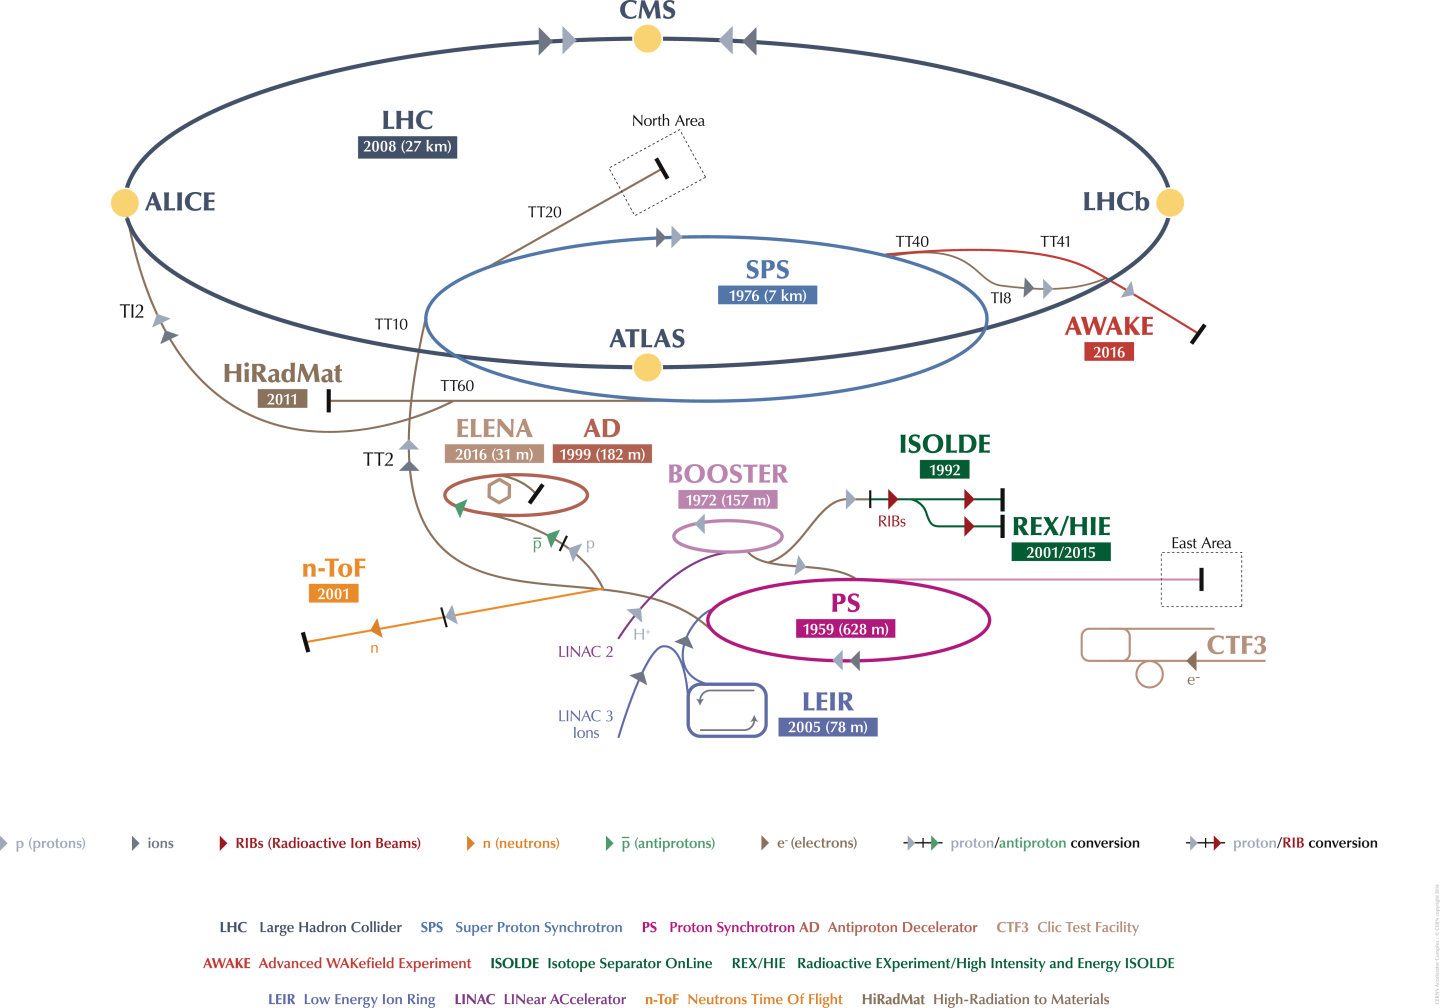
\includegraphics[width=1.1\textwidth]{01LHC/figs/accelerators.png}
  \end{center}
  \vspace{-2mm}
  \caption{Overview of the CERN accelerators complex.}
  \label{fig:accelerators}
\end{figure}

The LHC can also accelerate particles other than protons, such as lead or xenon nuclei, in order to collect data samples for specific studies.

%!TEX root = ../my_thesis.tex
\section{The LHCb experiment}
\label{sec:lhcb}

The \emph{Large Hadron Collider beauty} (LHCb) experiment~\cite{LHCb-DP-2014-002} is a single-arm forward spectrometer (see Fig.~\ref{fig:detector}) that exploits the forward production
of the $b$- and $c$- quark pairs in $pp$ collisions (Fig.~\ref{fig:angles}). The LHCb angular coverage is comprised between $15~\rm mrad$ and $250$ ($300$) $\rm mrad$ in the vertical (horizontal) plane.
The LHCb coordinate system consists of a right-handed set of axes, $x$, $y$, $z$, where the positive $z$ direction extends into the LHCb detector, $y$ is perpendicular to the LHCb cavern ground and $x$ is orthogonal to the other two.

\begin{figure}[htbp]
  \begin{center}
    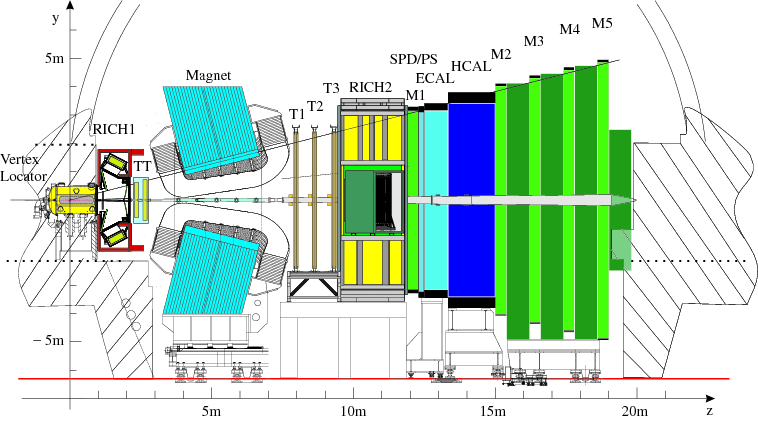
\includegraphics[width=0.9\textwidth]{02LHCb/figs/detector.png}
  \end{center}
  \vspace{-2mm}
  \caption{Side view of the LHCb detector.}
  \label{fig:detector}
\end{figure}

The LHCb experiment is composed of different sub-detectors. The tracking system includes a vertex and tracking detector called \emph{VErtex LOcator} (VELO), the \emph{Tracker Turicensis} (TT), located upstream a magnetic dipole with an integrated field of $4~\rm Tm$, the \emph{Inner Tracker} (IT), situated downstream the magnet in three separated stations around the beryllium beam pipe, and the \emph{Outer Tracker} (OT), installed in the same stations as the IT. The \emph{Particle IDentification} (PID) system comprises two \emph{Ring Imaging CHerenkov} detectors (RICH), an \emph{Electromagnetic CALorimeter} (ECAL), which also includes a \emph{Pre-Shower} (PS) and \emph{Scintillator Pad Detector} (SPD), a \emph{Hadronic CALorimeter} (HCAL) and five \emph{muon stations} (M1--M5).

\begin{figure}[htbp]
  \begin{center}
    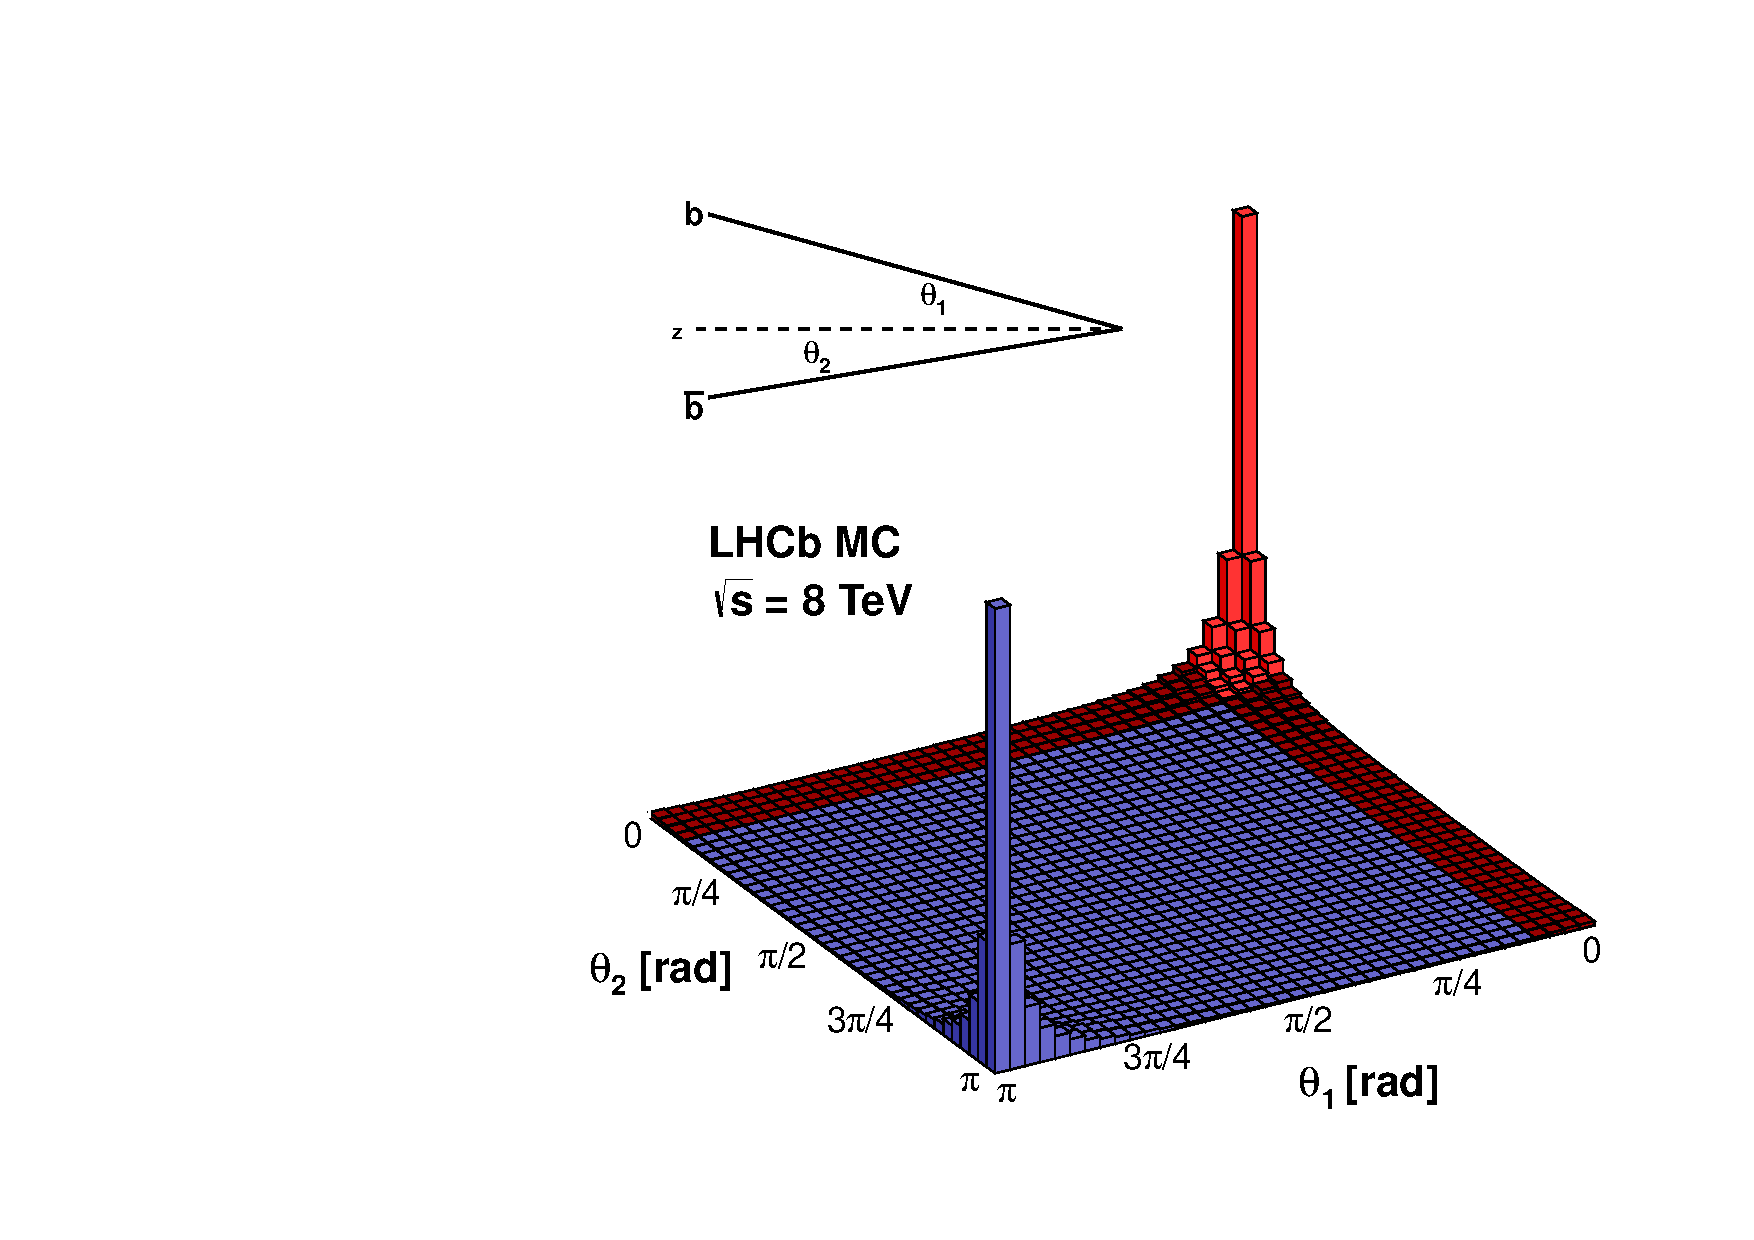
\includegraphics[width=0.5\textwidth]{02LHCb/figs/angles.pdf}
  \end{center}
  \vspace{-2mm}
  \caption{Joint distribution of the $b$ and $\bar b$ production angles with respect to the beam direction at $\sqrt{s}=8\rm~TeV$, as obtained from simulation. The red part shows the LHCb acceptance.}
  \label{fig:angles}
\end{figure}

\subsection{Tracking system}
\label{sec:tracking}

The tracking system plays a crucial role for the time-dependent analysis of $\Bz\to\Dmp\pip$ decays at LHCb.
The excellent vertex and impact-parameter resolution allows to separate true, long-lived $\Bz$ mesons from combinations of
other random tracks, and to improve the decay-time resolution.
Moreover, the optimal momentum resolution implies an excellent resolution on the reconstructed invariant mass, which is crucial
to separate true $\Bz\to\Dmp\pip$ decays from other physical background.

The tracking system is also essential for the flavour tagging algorithms, which rely on the quality of the reconstructed tracks and
vertices to discriminate correctly tagged neutral $B$ mesons from wrongly tagged ones.

A summary of the performances of the tracking system (momentum, impact-parameter, and decay-time resolution) is shown in Fig.~\ref{fig:track_perf}.

\begin{figure}[htbp]
  \begin{center}
    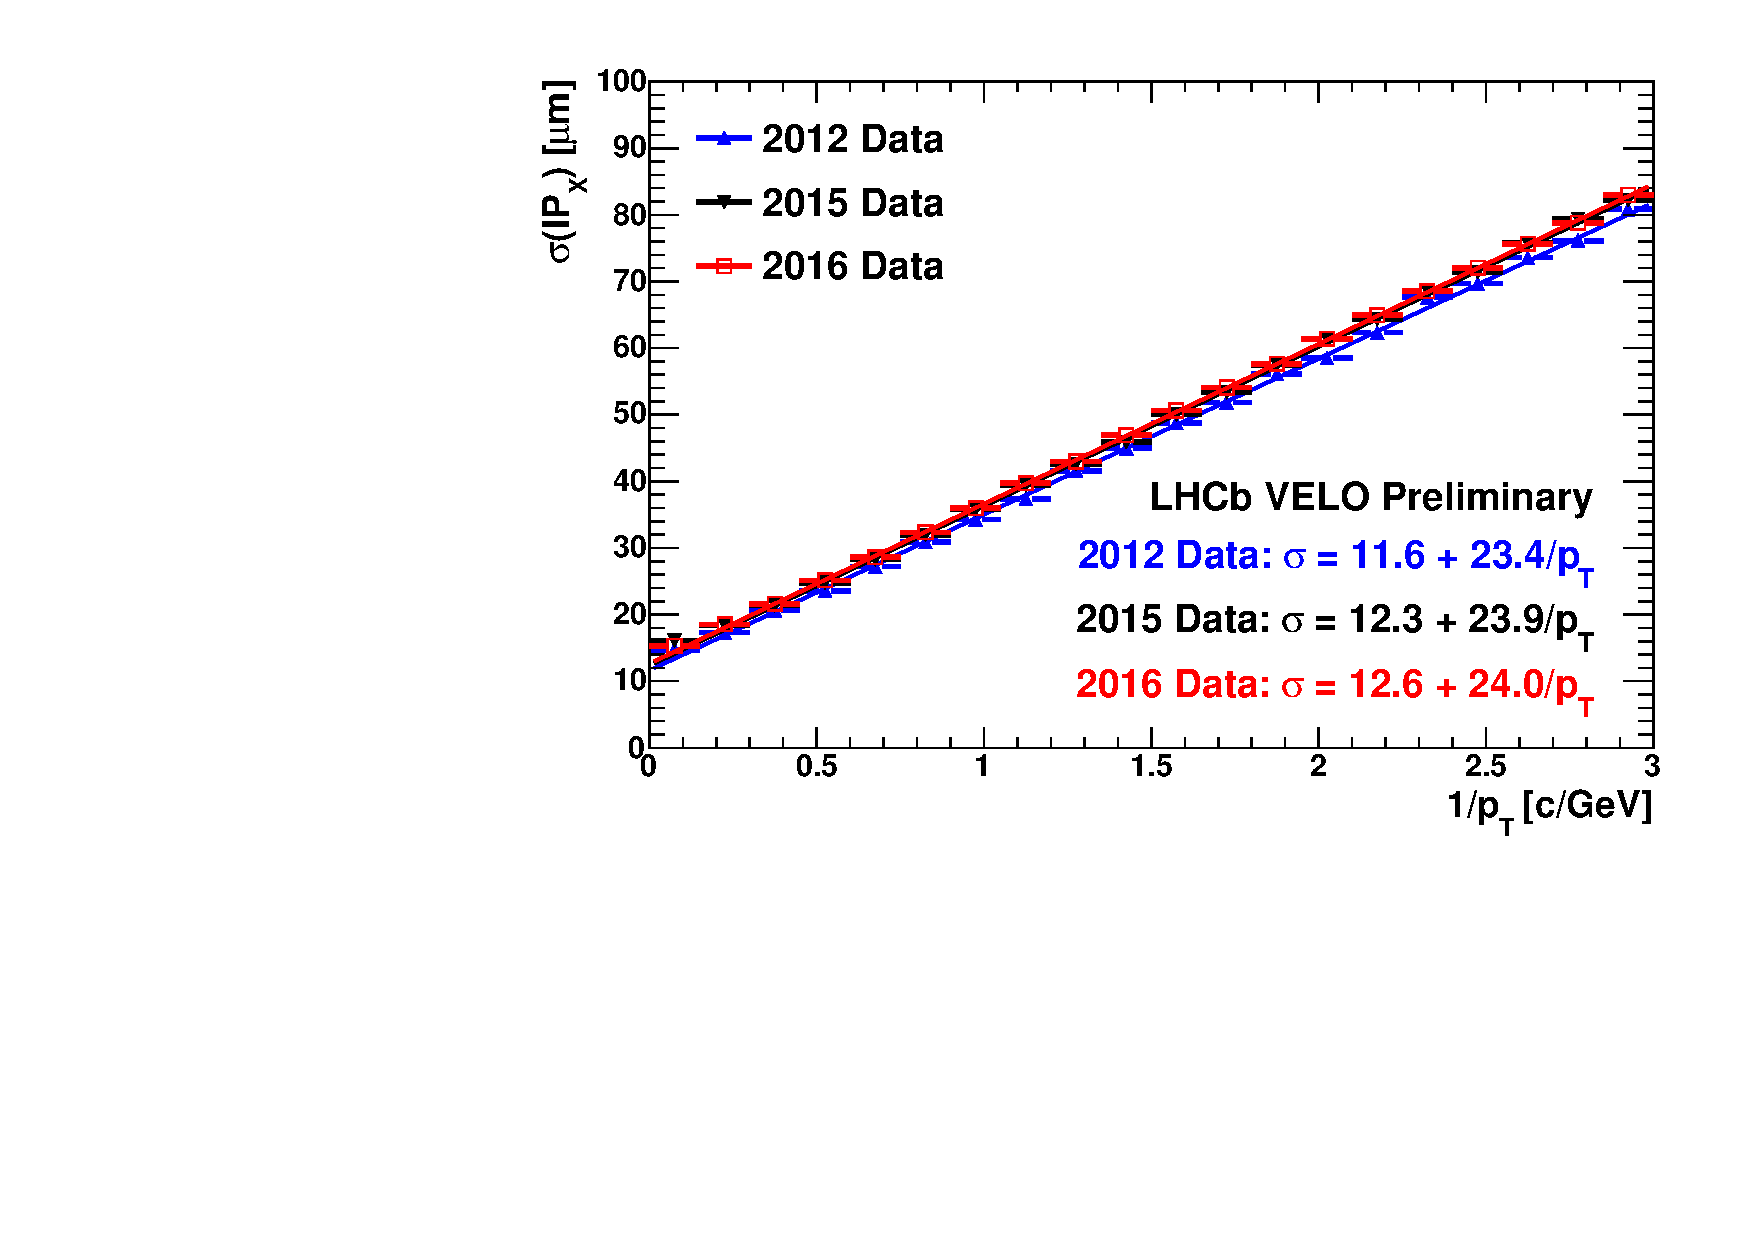
\includegraphics[width=0.48\textwidth]{02LHCb/figs/IPX-resolution.pdf}
    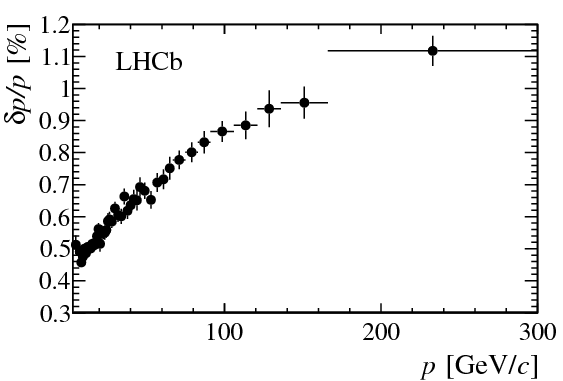
\includegraphics[width=0.48\textwidth]{02LHCb/figs/momentum_resolution.png} \\
    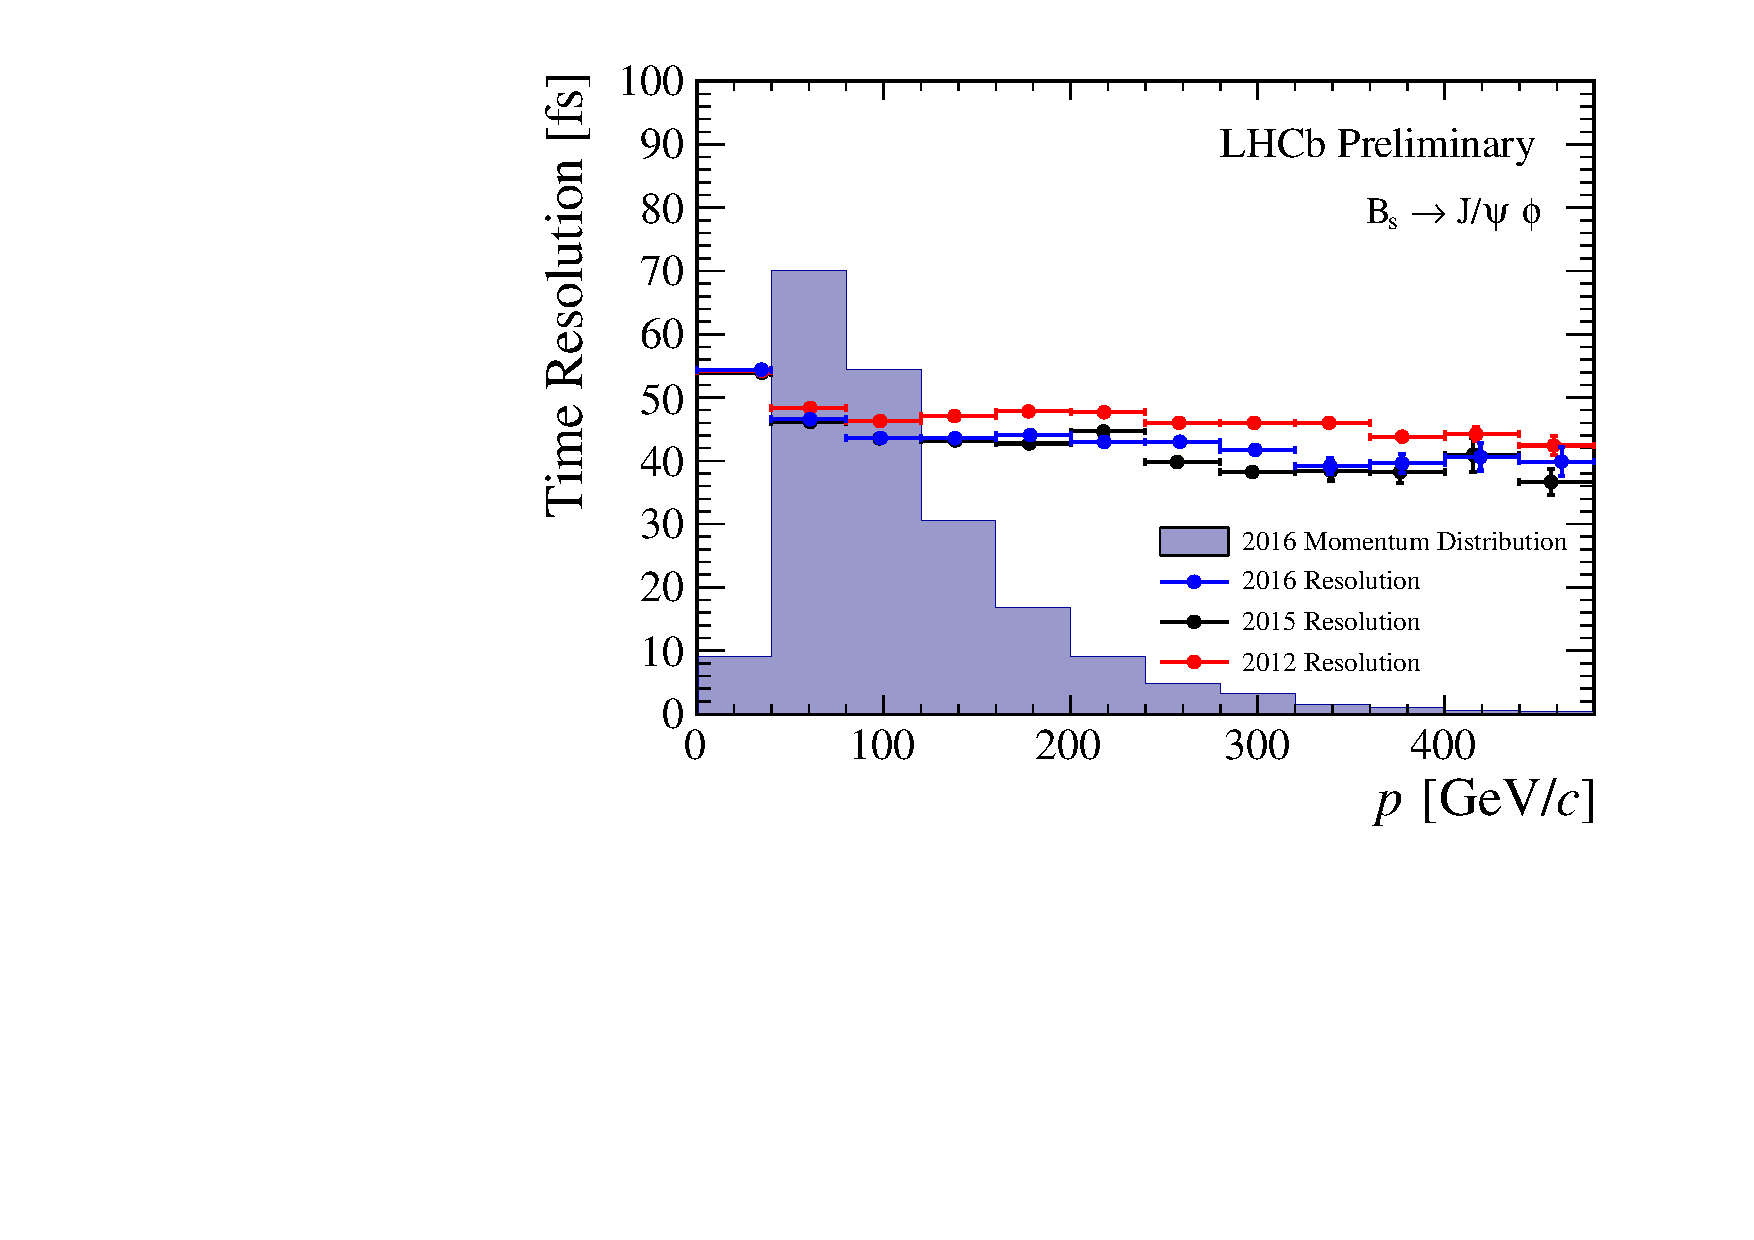
\includegraphics[width=0.48\textwidth]{02LHCb/figs/decay_time_res.pdf}
    \vspace{-5mm}
  \end{center}
  \caption{Top left: resolution on the $x$ coordinate of the impact parameter as a function of the inverse of the reconstructed transverse momentum in
  2012 (blue), 2015 (black) and 2016 (red) data. The result of a linear fit for each dataset is superimposed.
  Top right: relative momentum resolution as a function of the reconstructed momentum.
  Bottom: decay-time resolution as a function of momentum for reconstructed $\Bs\to J/\psi\phi$ decays in 2012 (red), 2015 (black) and
  2016 (blue) data. The momentum distribution is superimposed as the solid, purple histogram.}
  \label{fig:track_perf}
\end{figure}

\subsubsection*{The VErtex LOcator (VELO)}

The VELO \cite{LHCb-DP-2014-001} (Fig.~\ref{fig:VELO}) is a silicon micro-strip detector surrounding the interaction point, which detects charged particles, performs the first track reconstruction step and identifies decay vertices.
The sensitive region of the VELO is composed of n-on-n silicon micro-strip half-disk sensors with two different read-out strip geometries, called $r$-type and $\phi$-type, which measure the radial ($r$) and azimuthal ($\phi$)  position in polar coordinates. The silicon sensors are $8.4~\rm cm$ in diameter and have an inner hole with radius $0.8~\rm cm$. The strip pitch ranges from $38$ to $108~\rm\mu m$ ($38$ to $97~\rm\mu m$) for $r$ ($\phi$) sensors, while the sensor thickness is $300~\rm\mu m$.
The VELO consists of 21 stations placed perpendicular to the beam axis. Each station has two independent halves that can be moved apart during beam injection and then closed again when the beam orbit is stabilised. Each half-station is composed by one $r$-type and one $\phi$-type sensor. The total length of the VELO detector is about $1~\rm m$.
The impact parameter (IP) resolution of a track is measured to be $\sigma_{\rm IP}=11.6\pm23.4/\pt~\rm\mu m$ in $x$ and  $\sigma_{\rm IP}=11.2\pm23.2/\pt~\rm\mu m$ in $y$, where $\pt$ is the \emph{transverse momentum} (in $\gevc$) of the particle with respect to the beam axis. 

\begin{figure}[t]
  \begin{center}
    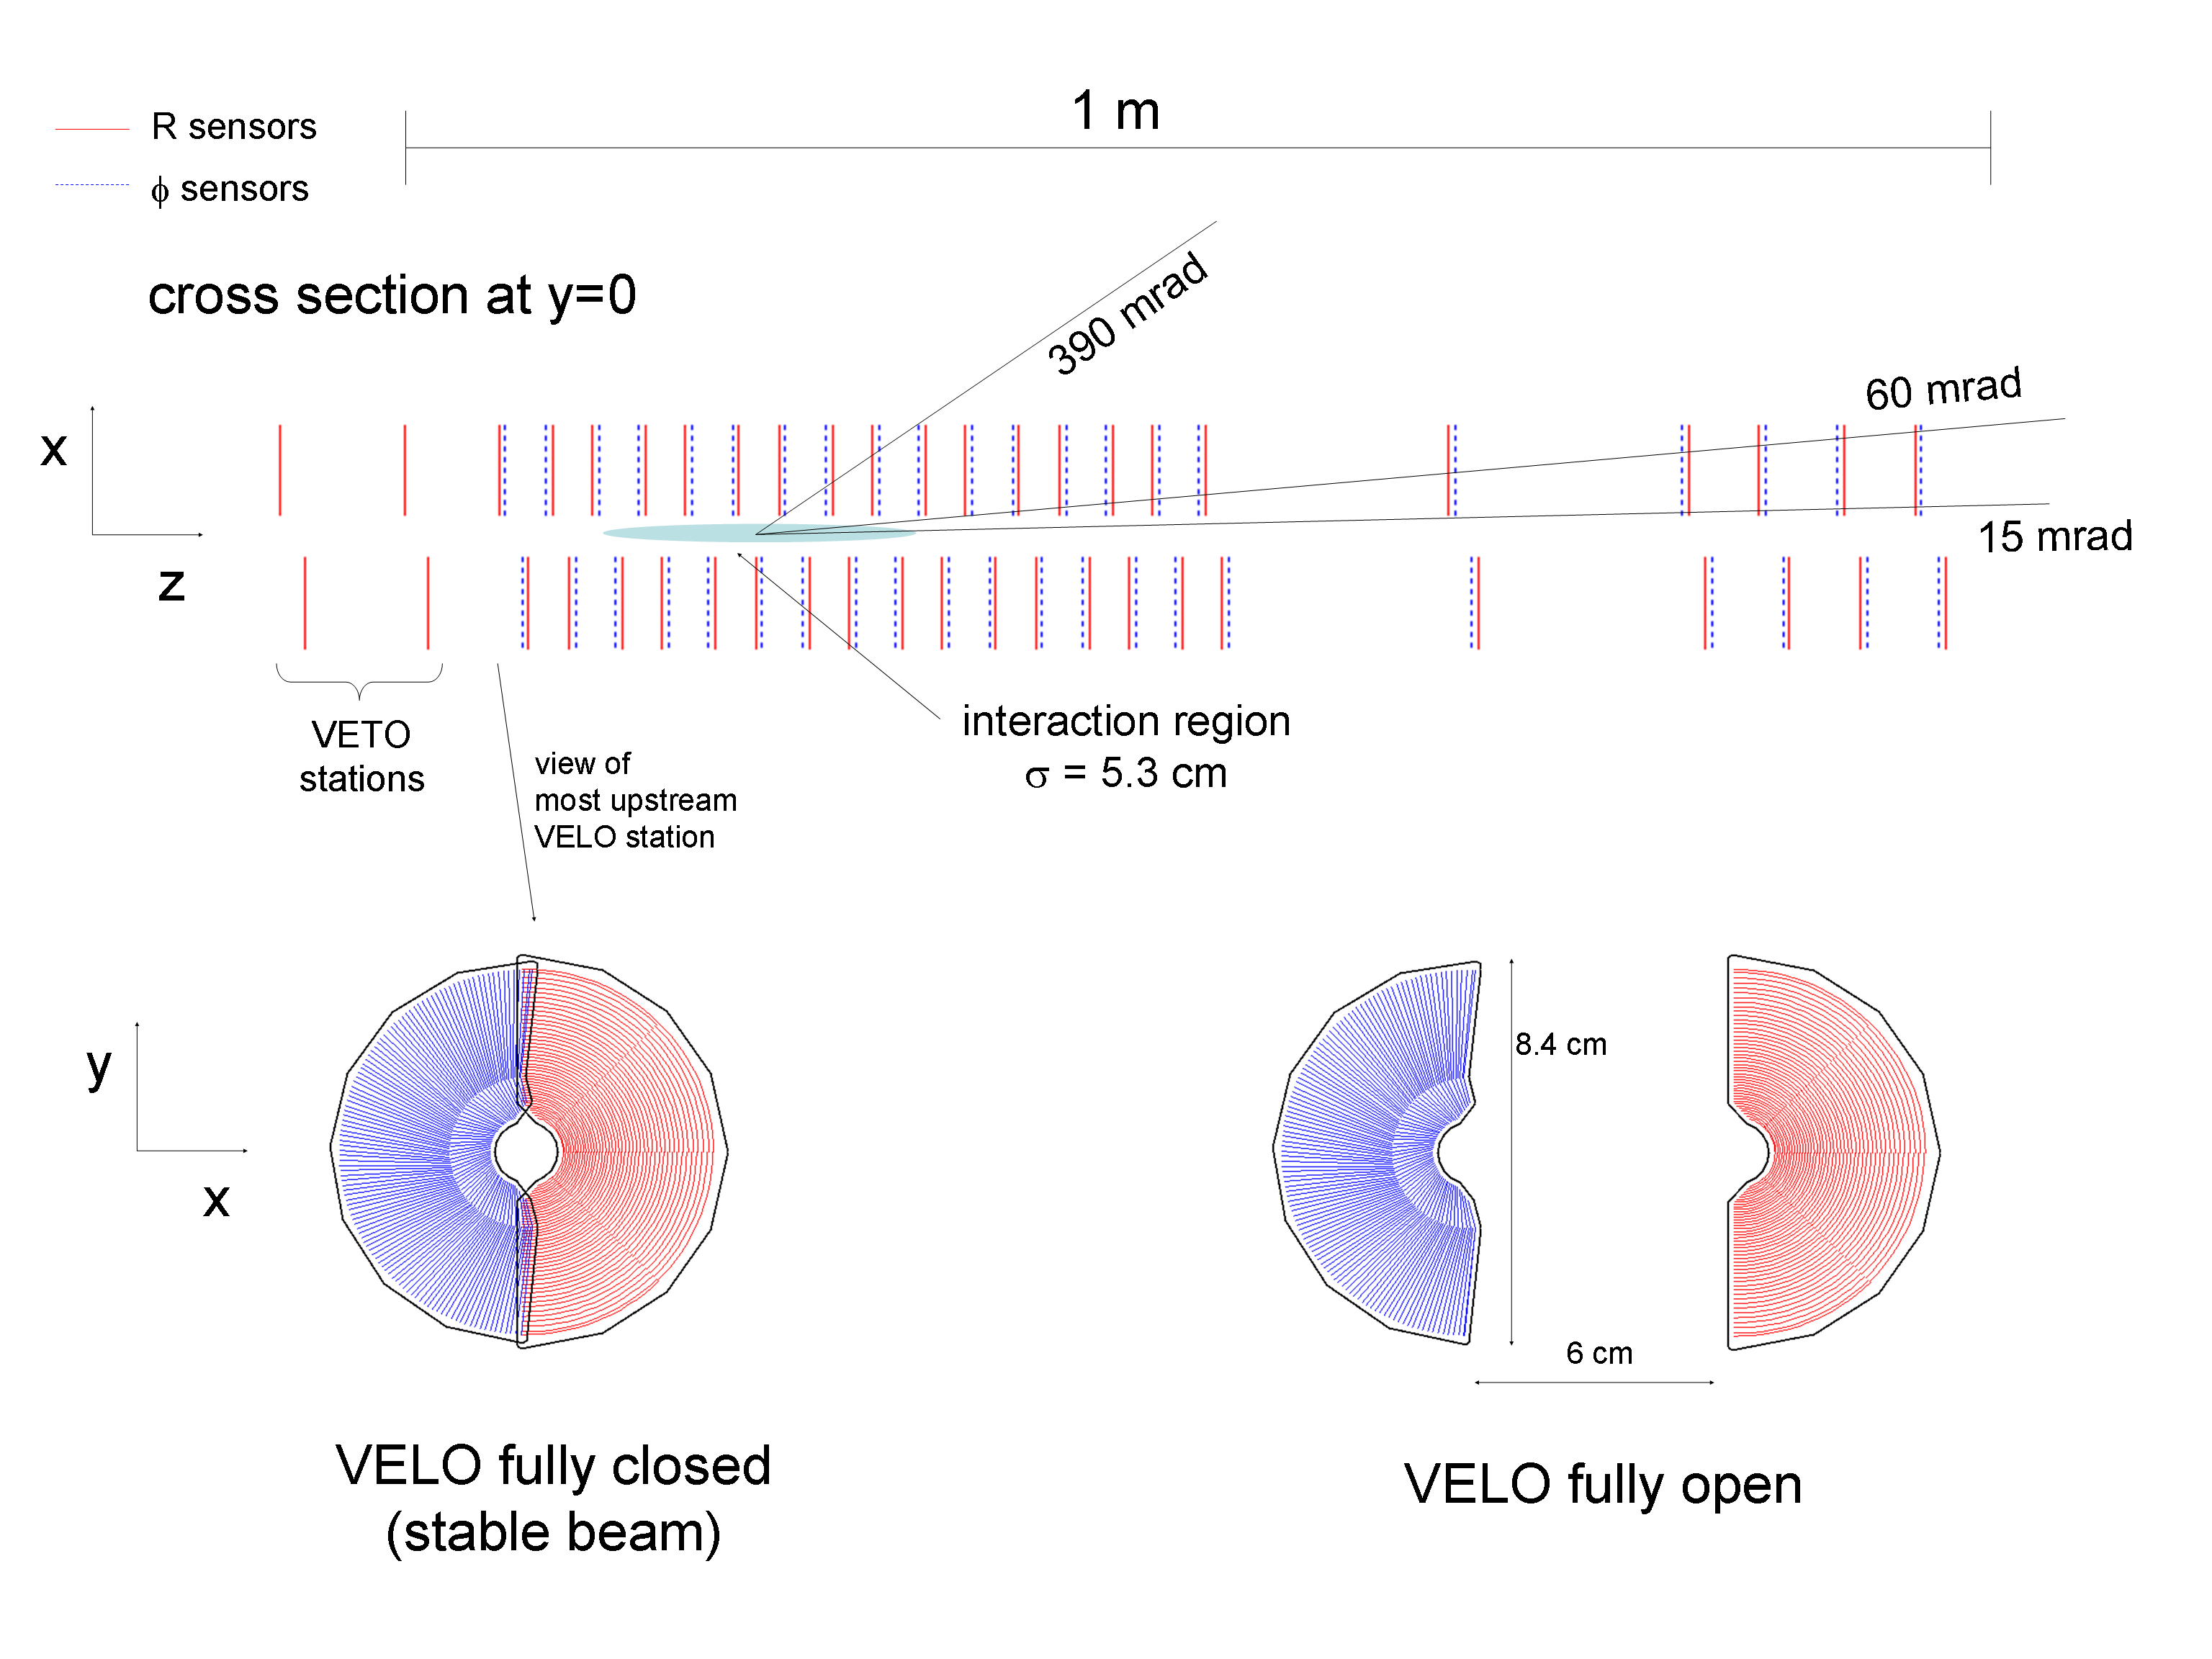
\includegraphics[width=0.9\textwidth]{02LHCb/figs/velo.png}
  \end{center}
  \vspace{-2mm}
  \caption{Schematic view of the VELO detector (top) and its sensors (bottom).}
  \label{fig:VELO}
\end{figure}

\subsubsection*{The Tracker Turicensis (TT)}

The TT \cite{LHCb-TDR-009} (Fig.~\ref{fig:TT}) is a silicon micro-strip detector covering a total area of about $7.9~\rm m^2$ upstream the magnet and divided into two separate stations (TTa, TTb). Each station has two layers. The TT helps in improving the track momentum resolution and detecting long-lived particles that decay outside the VELO acceptance. TTa is composed of a X and an U layer, while TTb includes a V and an X layer. The X layers have readout strips aligned vertically, whereas the U and V \emph{stereo} layers are rotated by $+5^{\degree}$ and $-5^{\degree}$ with respect to the vertical in the $xy$ plane.

\begin{figure}[t]
  \begin{center}
    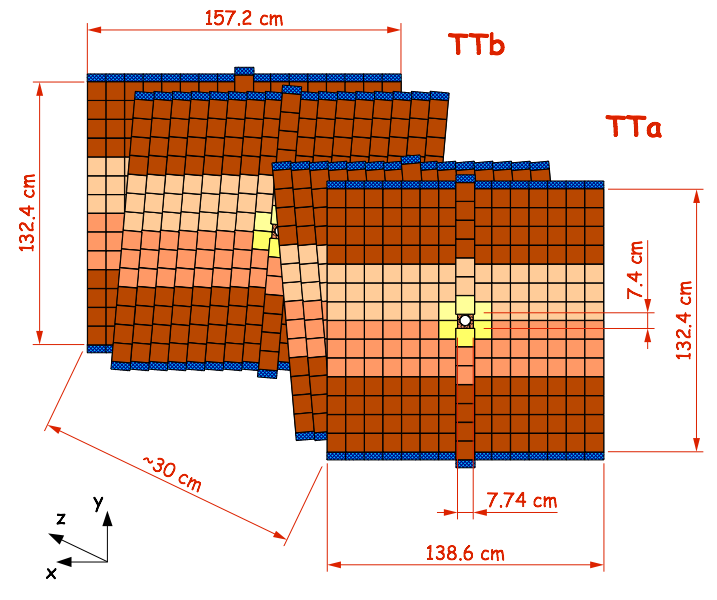
\includegraphics[width=0.4\textwidth]{02LHCb/figs/TT-scheme.png}
    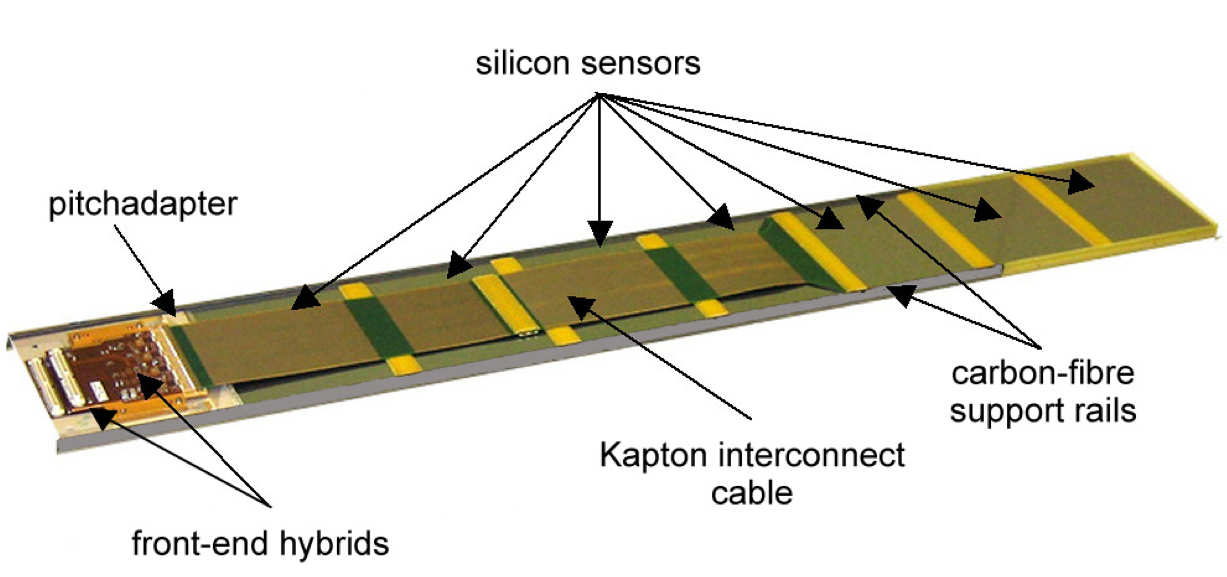
\includegraphics[width=0.4\textwidth]{02LHCb/figs/TT-strip-layout.png}
  \end{center}
  \vspace{-2mm}
  \caption{Schematic view of the TT stations/layers (left) and one of the TT readout modules (right).}
  \label{fig:TT}
\end{figure}


The TT active area is made of p-on-n silicon micro-strip sensors. Since the sensors are exposed to a significant radiation dose due to the high track multiplicity, they are cooled to $0^{\degree}$C in order to minimise the damage.

A TT readout module contains from one to four sensors connected in series, resulting in read-out strips up to $37~\rm cm$ long. The strip pitch is $183~\rm\mu m$ and the sensor thickness is $500~\mu m$. The hit resolution is about $50~\mu m$.

\subsubsection*{The Inner Tracker (IT)}

The IT \cite{LHCb-TDR-008} (Fig.~\ref{fig:IT}) is also a silicon micro-strip detector. Together with the TT, it forms the \emph{Silicon Tracker} (ST). It is dedicated to detect charged particles in the high track-density region around the beam pipe downstream the magnet. It is separated into three stations, where each station consists of four boxes. Each box has four layers made of seven read out modules arranged in a X-U-V-X layout similar to that of the TT.
The total coverage of the IT is about $4.2~\rm m^2$. The boxes directly above and below the beam pipe are made of single-sensor modules, called \emph{short modules}, whereas the side boxes are made of two bonded silicon sensor modules, called \emph{long modules}. The IT strip pitch is $198~\rm\mu m$, while the p-on-n sensor thickness is $320$ ($410$) $\mu m$ for the short (long) modules. The hit resolution is about $50~\rm\mu m$.

\begin{figure}[t]
  \begin{center}
    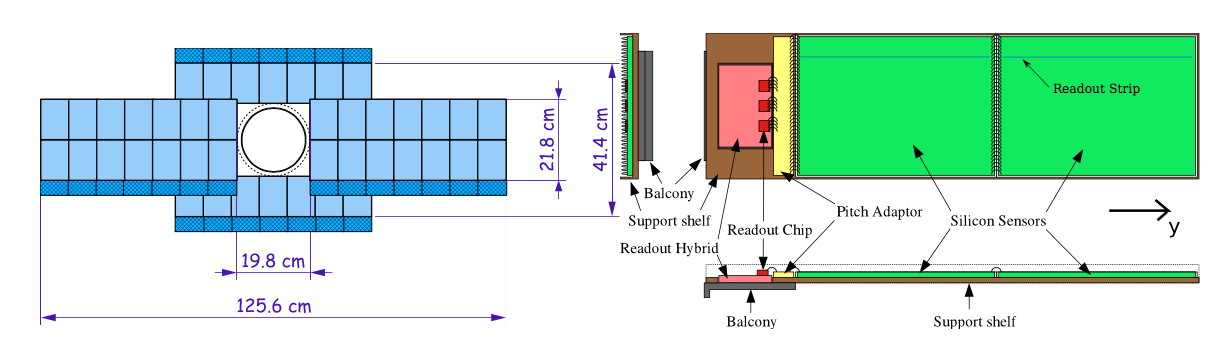
\includegraphics[width=0.9\textwidth]{02LHCb/figs/IT.png}
  \end{center}
  \vspace{-2mm}
  \caption{Schematic view of an IT station (left) and one of the long IT readout modules (right).}
  \label{fig:IT}
\end{figure}

\subsubsection*{The Outer Tracker (OT)}

The OT \cite{LHCb-TDR-006} (Fig.~\ref{fig:OT}) is a gaseous straw-tube detector filled with an Ar/$\rm CO_2$/$\rm O_2$ ($70\%/28.5\%/1.5\%$) gas mixture. It is dedicated to the detection of charged particles in the low track density region outside the IT acceptance and covers a large area of about $340~\rm m^2$. The OT is composed of three stations, where each station has four layers in a X-U-V-X configuration. Each station is separated physically in left and right sides with respect to the beam pipe mounted in support structures called C frames because of their shape. Each layer is divided into two mono-layers. The OT has different types of modules, the long F modules and the short S1, S2, S3 modules that are cut in two pieces to leave space for the IT. The straw tube and anode wire diameters are $5~\rm mm$ and $25~\rm\mu m$ respectively. The hit resolution is about $200~\mu\rm m$.

\begin{figure}[t!]
  \begin{center}
    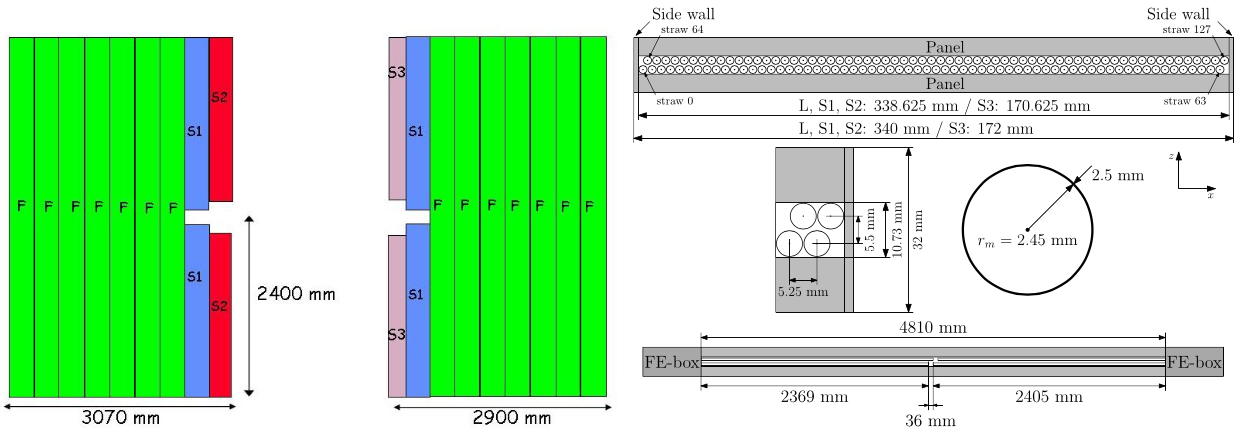
\includegraphics[width=0.9\textwidth]{02LHCb/figs/OT.png}
  \end{center}
  \vspace{-2mm}
  \caption{Schematic view of an OT layer (left) and an OT module layout (right).}
  \label{fig:OT}
\end{figure}

\subsubsection*{Spillover noise in the Silicon Tracker}

Starting from 2015, the time spacing between the LHC proton \emph{bunches} has been $25~\rm ns$, half of the value adopted before. This had a direct impact on the front-end electronics of the silicon detectors (VELO, TT, IT), because the width in time of the analogue signal produced by the front-end electronics is of the same order of magnitude. This means that it is possible to still have a non negligible amount of signal in the subsequent collision, which can be misidentified as coming from particles produced in that event. This source of noise is called \emph{spillover}. The starting seeds of tracking algorithms, called \emph{clusters}, can be polluted by spillover clusters which may increase the number of fake (or \emph{ghost}) reconstructed tracks. 

In the first part of my PhD activity, I studied the effect of splillover clusters in the ST using both simulated events and real collision data. This study shows that this time spacing has little impact on the detector \emph{occupancy}, and that the increase of ghost tracks is negligible. Moreover, it is shown that the charge deposited by particles in the detector can be exploited as a \emph{feature} in multivariate analyses in order to further reduce the ghost track contamination. These results are documented in a note~\cite{spillover} internal to the LHCb collaboration.

\subsection{Particle identification (PID)}
\label{sec:pidintro}

\subsubsection*{The Ring Imaging CHerenkov (RICH) detectors}

When a charged particle is travelling faster than the speed of light in a medium, Cherenkov light is produced at an angle that depends on the velocity of the particle and the refractive index of the medium (\emph{radiator}). By knowing the momentum from the tracker and the velocity from the RICH detectors, the mass can be determined and therefore provide particle identification. Two RICH detectors \cite{RICH} (Fig.~\ref{fig:RICH}) are used in order to provide PID in different momentum ranges.

RICH1 is responsible for providing PID in the momentum range from $1$ to $60\gevc$. The angular acceptance ranges from $25$ to
$50$ ($300$) $\rm mrad$ in the vertical (horizontal) plane. The adopted radiator is fluorobutane ($\rm C_4 F_{10}$). RICH1 is located between the VELO and the TT. 
The Cherenkov photons are guided to Hybrid Photon Detectors (HPD) via dedicated mirrors.

The average kaon identification efficiency in the momentum range from $2$ to $100\gevc$ is $\sim95\%$. The average probability that pions are wrongly identified as kaons is $\sim5\%$ in the same momentum range.

\begin{figure}[t]
  \begin{center}
    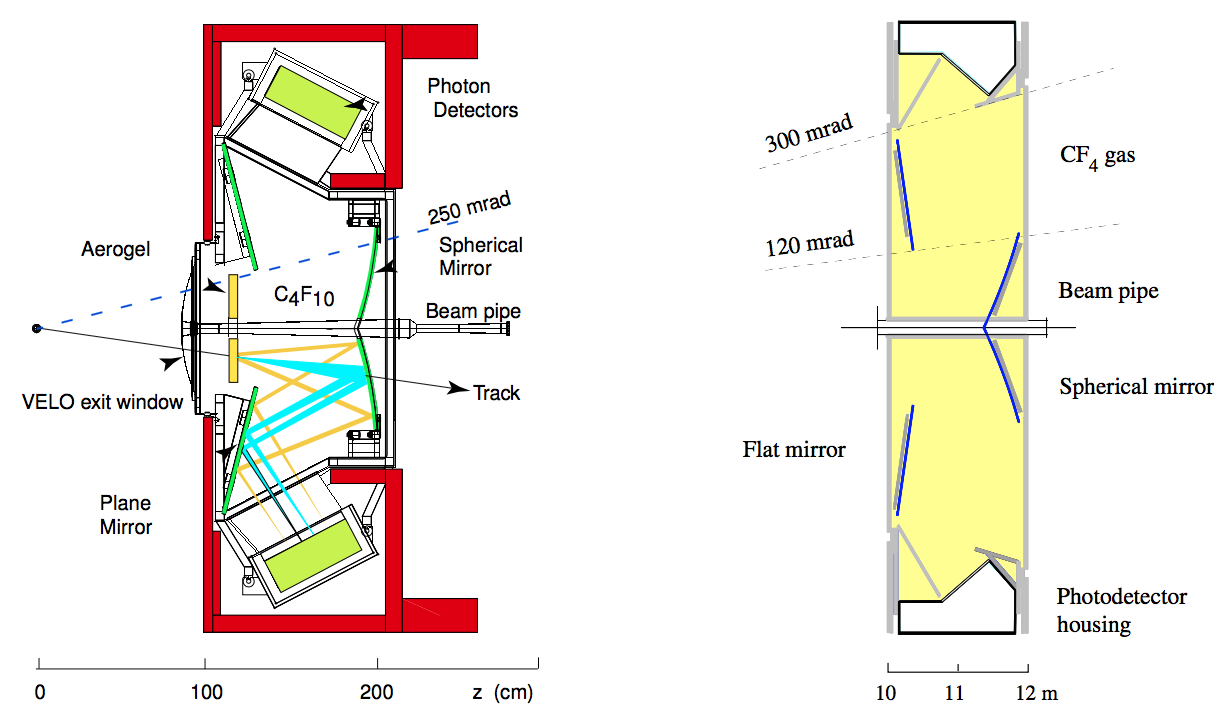
\includegraphics[width=0.8\textwidth]{02LHCb/figs/RICH.png}
  \end{center}
  \vspace{-2.5mm}
  \caption{Side view of RICH1 (left) and top view of RICH2 (right).}
  \label{fig:RICH}
\end{figure}

RICH2 is optimised for the momentum range from $15$ to $100\gevc$. The angular acceptance ranges from $15$ to $100$ ($120$) $\rm mrad$ in the vertical (horizontal) plane where most of the high-momentum tracks are produced. RICH2 uses tetrafluoromethane ($\rm CF_4$) as radiator.

\subsubsection*{The Electromagnetic CALorimeter (ECAL), Pre-Shower (PS) and Scintillator Pad Detector (SPD)}

The ECAL \cite{CAL} is used for the detection and measurement of the energy of electrons and
photons. The ECAL is built as a sandwich of alternating scintillators and
lead layers in the $xy$ plane. Scintillation light produced by the shower of
particles generated by the lead plates is read out by Wave-Length Shifter (WLS) fibres coupled
to PhotoMultiplier Tubes (PMTs). The SPD is installed upstream the ECAL to separate electrons
from photons. The PS is installed between the SPD and
the ECAL. Both SPD and PS use scintillator
pads read out by WLS fibres coupled to MultiAnode PhotoMultiplier Tubes (MAPMT). The
acceptance range of the ECAL is from $25$ up to $300$ ($250$) $\rm mrad$ in the horizontal (vertical) 
plane. The relative energy resolution of the ECAL is given by $\sigma_E / E = 10\%/\sqrt{E}\oplus 1\%$, where $E$ is given
in$\gev$.

\subsubsection*{The Hadronic CALorimeter (HCAL)}

The HCAL \cite{CAL} is used for the detection and measurement of the energy of hadrons 
for the first level trigger. A HCAL cell is a sampling device made of
alternating iron and scintillator tiles, where the latter are located along the beam direction. The HCAL
has the same acceptance coverage of the ECAL. The relative energy resolution of the HCAL
is given by $\sigma_E / E = (69\pm 5)\%/\sqrt{E}\oplus (9\pm 2)\%$, where $E$ is given in$\gev$. 

\subsubsection*{Muon detectors}

The muon system \cite{MUON} (Fig.~\ref{fig:MUON}) is a gaseous detector composed of five stations (M1 to M5) interleaved by $80~\rm cm$ thick iron filters. The gaseous detectors are Multi-Wire Proportional Chambers (MWPC), except for the innermost part of M1, where triple Gas Electron Multipliers (GEM) detectors are used to cope with the higher track density. The angular acceptance ranges from $20$ ($16$) to $308$ ($256$) $\rm mrad$ in the horizontal (vertical) plane. The muon detector has $1380$ chambers and covers a total area of $435~\rm m^2$. Each muon chamber is composed of four layers of MPWC, except for M1, where two layers are used. The hit efficiency of the chambers is higher than $99\%$ enabling a trigger efficiency greater than $95\%$ for muons. The adopted gas mixture ($40\%$~Ar, $55\%~\rm CO_2$, $5\%~\rm CF_4$) allows a fast triggering on muons ($40~\rm MHz$).

\begin{figure}[t!]
  \begin{center}
    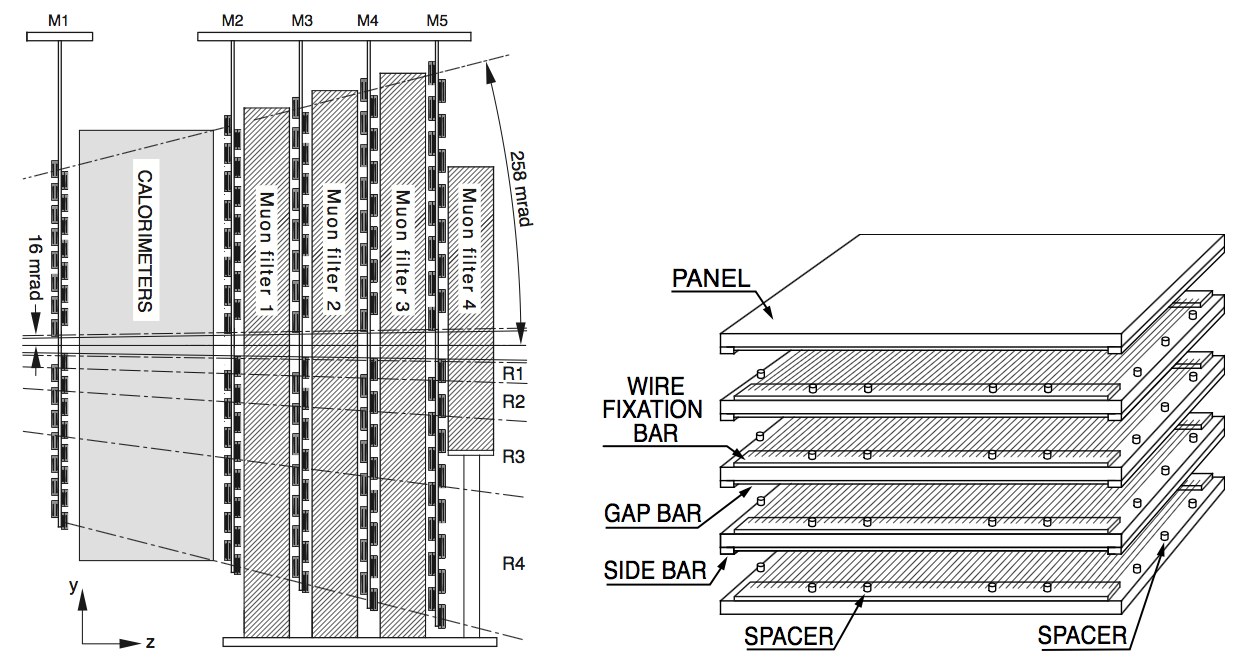
\includegraphics[width=0.9\textwidth]{02LHCb/figs/MUON.png}
  \end{center}
  \vspace{-2mm}
  \caption{Schematic view of the muon system (left) and a MWPC (right).}
  \label{fig:MUON}
\end{figure}

\subsection{Trigger system}

The bunch crossing rate of LHC is very high ($40~\rm MHz$) because more than $99\%$ of the $pp$ collisions do not produce interesting events. It is not possible to record events with such a high rate: therefore, a trigger system \cite{Trigger} is required to reduce the rate from $40~\rm MHz$ down to a few $\rm kHz$. The rate reduction is achieved via selection criteria which ensure that events containing heavy flavour decays are stored. The signatures of these interesting decays include high transverse momentum ($\pt$) and transverse energy ($E_{\rm T}$) of the decay products, as well as displaced decay vertices 
or tracks with large impact parameter (IP) with respect to the $pp$ collision point due to the relative long lifetimes of $b$ and $c$ hadrons. The trigger is divided into two sequential stages: a hardware stage called Level-0 (L0) trigger, and a software stage called High Level Trigger (HLT). Different trigger decisions are separated into various \emph{lines}, each of which provides information on different physics processes (\eg~decay topology, presence of muons etc\dots). All the trigger steps are summarised in Fig.~\ref{fig:trigger}.

Two types of trigger response are assigned offline, when some physics channel is analysed. The TOS (\emph{Trigger On Signal}) trigger occurs when the presence of the signal is sufficient to have a positive trigger decision. The TIS (\emph{Trigger Independent of Signal}) trigger occurs when, after removing signal tracks and hits associated to them, another signature in the event is sufficient to have a positive trigger decision.

After the trigger stage, the data go through further offline selection steps, where exclusive (\eg~$\B\to \Dmp\pipm$, $\Bpm\to J/\psi K^{\pm}$) and inclusive (\eg~$b$~hadron~$\to J/\psi X$, $J/\psi\to\mu^+\mu^-$) decays are reconstructed at higher quality than was possible in the strict timing requirements of the trigger, and further selections are applied.
This offline selection step is known as \emph{stripping}, and each set of selection requirements is called \emph{stripping line}.

\begin{figure}[htbp]
  \begin{center}
    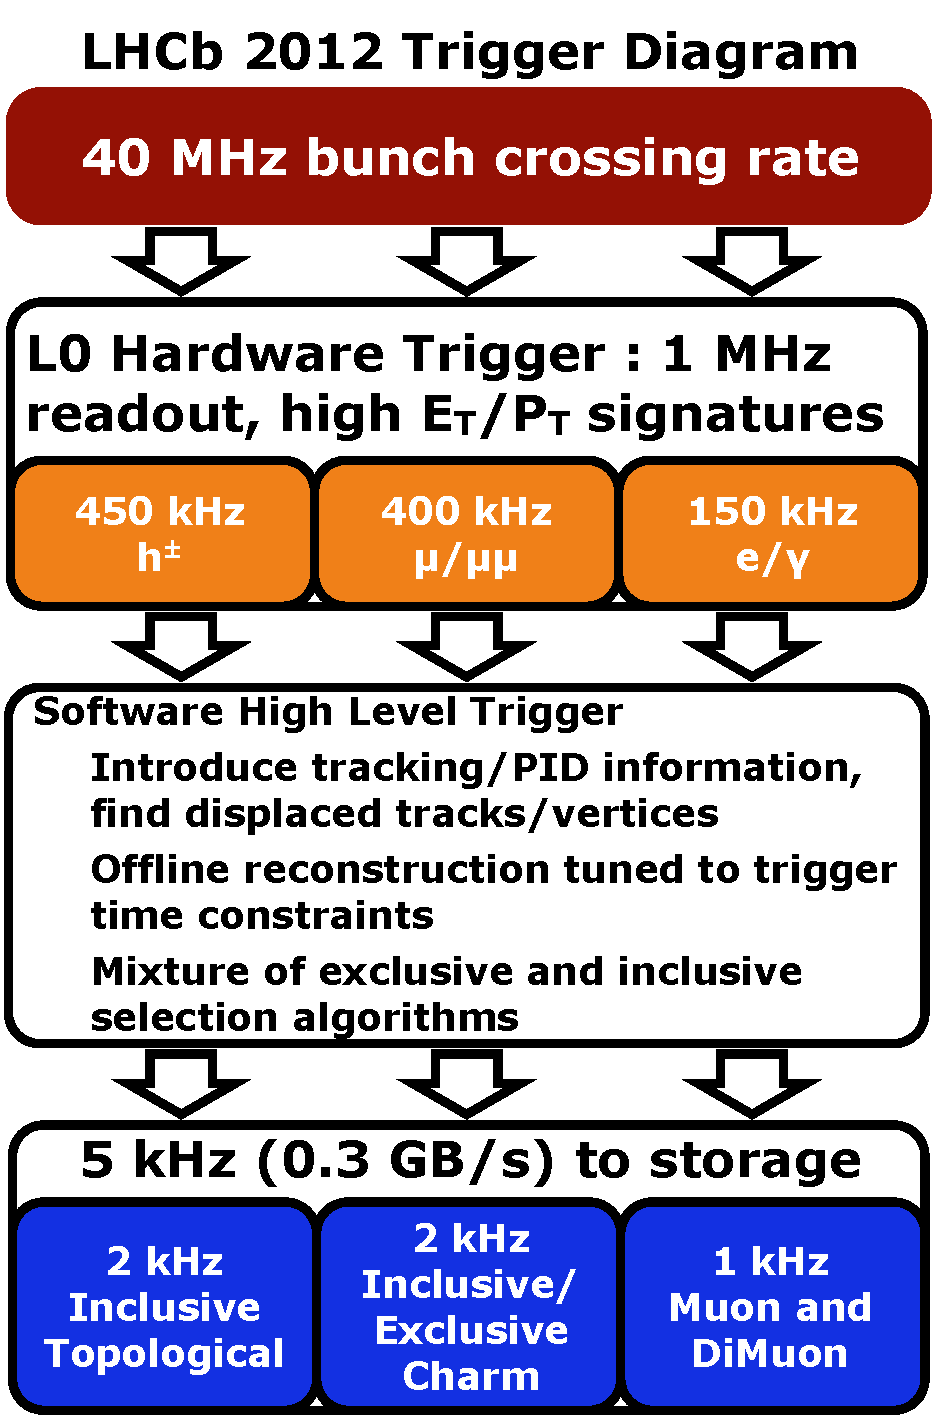
\includegraphics[width=0.45\textwidth]{02LHCb/figs/TriggerRunI.pdf}
    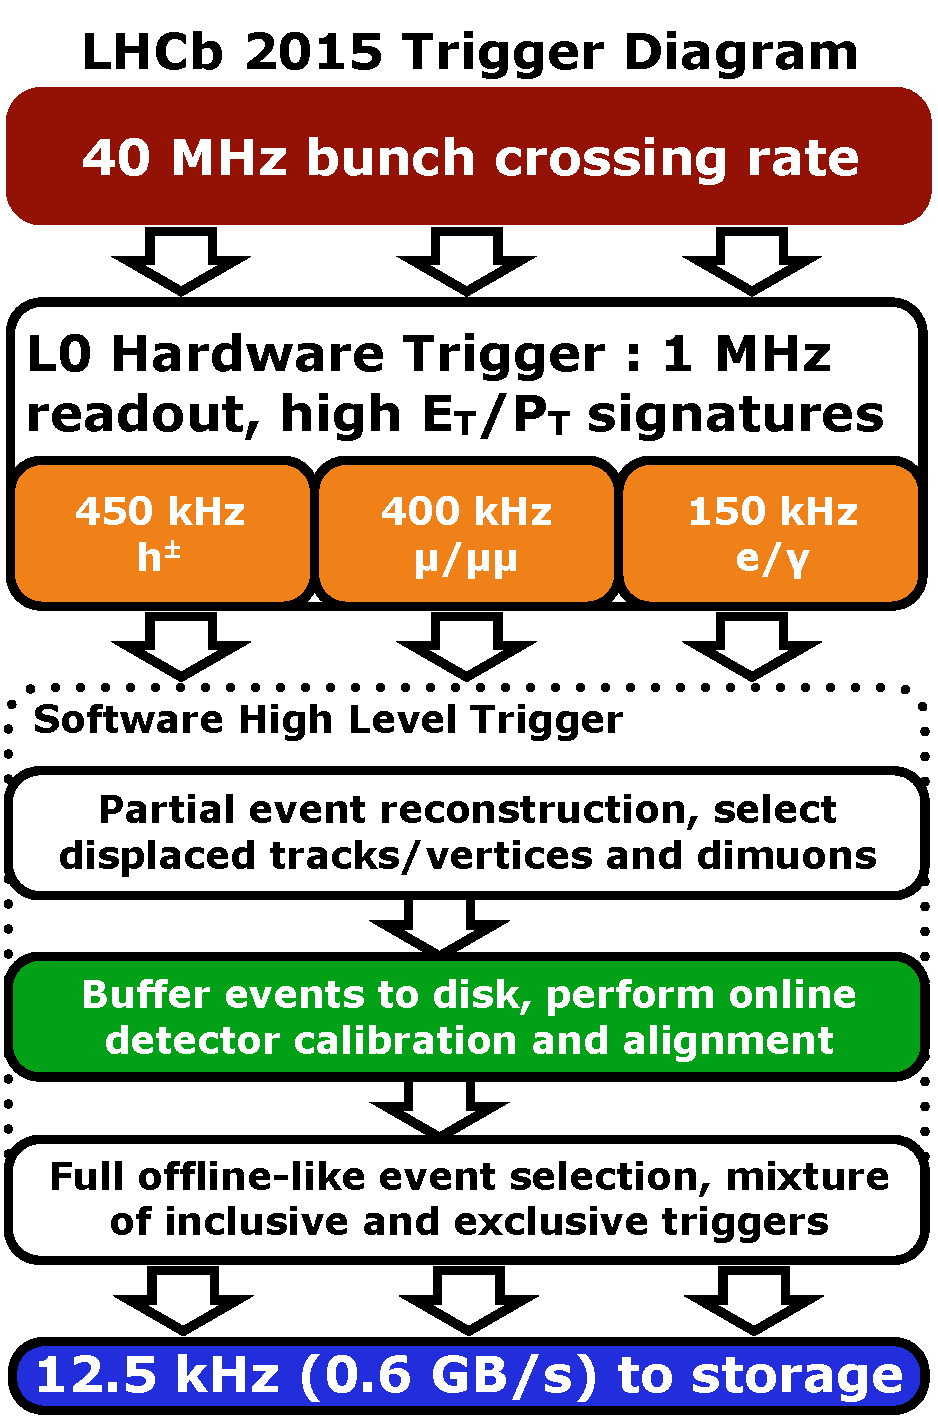
\includegraphics[width=0.45\textwidth]{02LHCb/figs/TriggerRunII.pdf}
  \end{center}
  \vspace{-2mm}
  \caption{Summary of the trigger strategies followed during the Run 1 (2011--2012, left) and Run 2 (2015--2017, right) data-taking periods. During Run 2, an online detector and calibration alignment was introduced, as well as full event selections (both inclusive and exclusive).}
  \label{fig:trigger}
\end{figure}

\subsubsection*{Level-0 trigger (L0)}

The L0 mainly exploits the calorimeters and muon chambers. The idea behind the L0 is to select events that contain high \pt~muons and high $E_{\rm T}$ hadrons, electrons and photons, which very likely come from $b$- and $c$-hadron decays, by using simple signatures that do not require the reconstruction of the event.
The L0 reduces the data rate from $40~\rm MHz$ down to $1~\rm MHz$, which is the rate limit of the LHCb readout electronics.

\subsubsection*{High Level Trigger (HLT)}

The HLT is separated into two stages, HLT1 and HLT2, and runs on about $29\,000$ commercial CPU cores. 

At the HLT1 level, the full detector information is read out, and then track/vertex reconstruction and PID are performed. The exploited signatures are mainly the presence of high \pt~tracks, high transverse energy calorimeter clusters (photons and $\pi^0$), high invariant mass of muon pairs, and tracks with large IP. All the HLT1 trigger lines are \emph{inclusive}, meaning that only decay products common to various decay processes are selected rather than specific decays. After the HLT1, the rate goes down to about $70~\rm kHz$.

The HLT2 is a combination of inclusive selections and algorithms that reconstruct entirely (\emph{exclusively}) some decay processes. The main lines are topological lines using Multi-Variate Analysis (MVA) techniques with different sets of kinematic and position features as input, exclusive charm lines and high mass displaced di-hadron/lepton lines. After the HLT2, the events are stored on tape for further offline analysis.

\subsection{Event reconstruction and simulation}

\subsubsection*{Track and vertex reconstruction}

Starting from the \emph{hits} in the tracking detectors, tracks and vertices are reconstructed via dedicated algorithms. 
Different track types are reconstructed, as shown in Fig.~\ref{fig:trackTypes}. Each track is characterised by hits collected in different sub-detectors. For example, downstream tracks, with no hits in the VELO,
are typically associated to long-lived particles such as $\Lambda$ and $K^0_{\rm S}$. Because of the vertical magnetic field, tracks are bend in the $xz$ plane. By knowing the reconstructed particle trajectory and 
the magnetic field map, it is possible to measure the momentum of the particle.

\begin{figure}[htbp]
  \begin{center}
    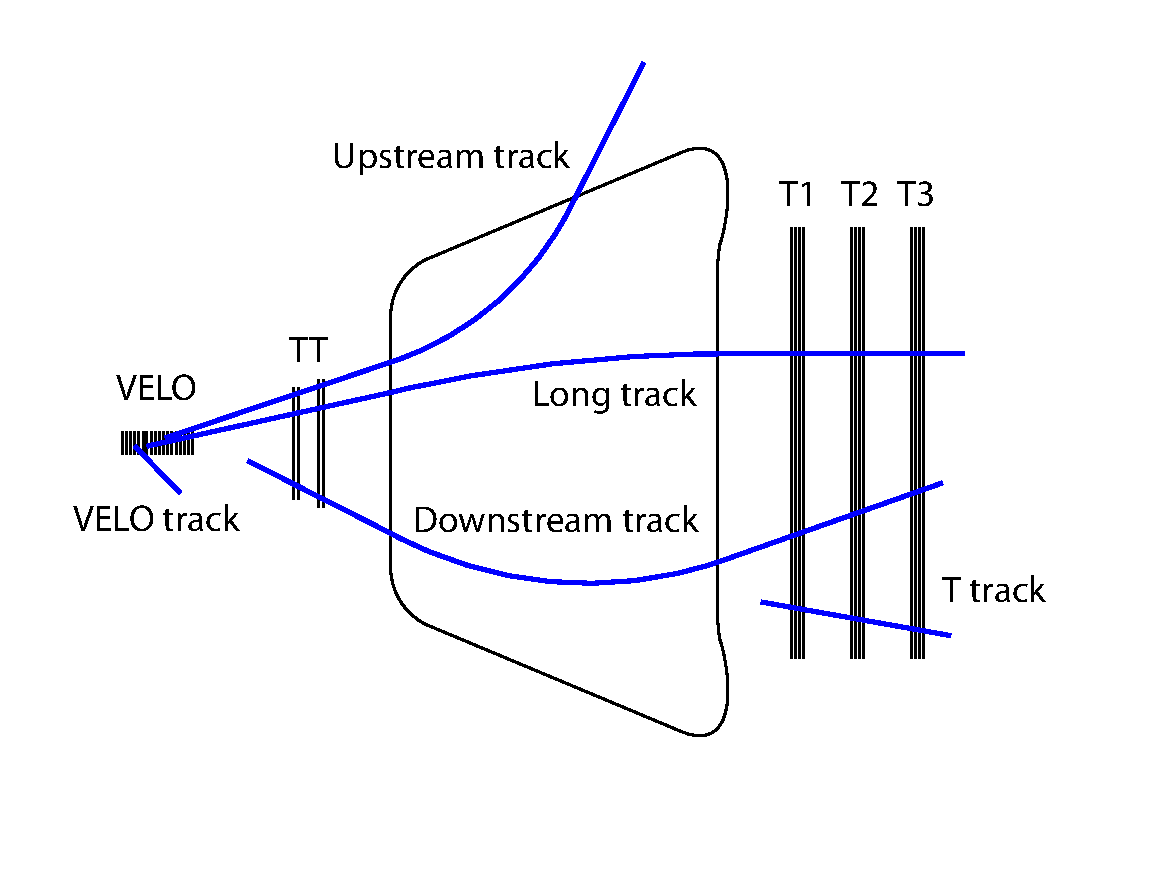
\includegraphics[width=0.9\textwidth]{02LHCb/figs/trackTypes.pdf}
  \end{center}
  \vspace{-15mm}
  \caption{Schematic description of the different track types reconstructed in LHCb.}
  \label{fig:trackTypes}
\end{figure}

\subsubsection*{PID}
The Cherenkov radiation emitted by charged particles in the RICH radiators produces \emph{rings} in the RICH acceptance, which are reconstructed via pattern recognition algorithms.
For each reconstructed pattern, the \emph{likelihood} $\mathcal L_{\pi}$ for the ring to be produced by a pion (the most common particle in the LHCb environment) is computed.
The momentum of the particle is also used in the likelihood computation.
Then, likelihood functions for other hypotheses (kaon, proton, electron, muon) are computed and compared with the pion likelihood.
For a given particle X (X=$e,\mu,p,K$), the PIDX observable is defined as
\begin{equation}
	\label{eq:pidx}
	\rm PIDX = \ln \mathcal L_{\rm X} - \ln \mathcal L_{\pi}.
\end{equation}
In typical LHCb analyses, requirements on the PID observables are applied to suppress physical backgrounds due to wrongly-identified particles.
The PID observables are adopted, together with other kinematic and detector-related observables, as input feature for neural networks which predict the probability for a
particle to be either an electron, a muon, a proton, a kaon, or a pion. This probability is denoted as PROBNNX (X=$e,\mu,p,K,\pi$).

\subsubsection*{Simulation}
The Monte Carlo (MC) simulation of $pp$ collisions, particle decays, and interactions with the detector are crucial in the validation of physics analyses.
The parton-parton collision and hadronisation simulation is performed by \texttt{PYTHIA}~\cite{Sjostrand:2007gs}, interfaced to \texttt{EvtGen}~\cite{Lange:2001uf} for the decay of the hadrons and leptons for standard productions. The QED corrections to the decay (\ie~the emission of radiation photons) is generated by the \texttt{PHOTOS} package~\cite{Golonka:2005pn}. The interactions of particles with the detector material and their tracking in the magnetic field are simulated by \texttt{GEANT4}~\cite{Agostinelli:2002hh,Allison:2006ve}.

\subsection{Data collected by LHCb}
\label{sec:lhcdata}

The collision rate $R$ $[\rm s^{-1}]$ in LHC can be expressed in terms of the \emph{cross-section} $\sigma$ $[\rm cm^2]$ and the \emph{luminosity} $\mathcal L$ $[\rm s^{-1} \rm cm^{-2}]$ as
\begin{equation}
	R = \mathcal L \sigma.
\end{equation}
For a given data-taking period, the \emph{integrated luminosity} $L~[\rm cm^{-2}]$ is a measure of the amount of recorded data. The typical unit for luminosity is the inverse \emph{barn}, which corresponds to $10^{24}~\rm cm^{-2}$. The LHCb integrated luminosity is of the order of an inverse \emph{femtobarn} ($\rm fb^{-1}$); one inverse femtobarn corresponds to the production of about $10^{11}$ $b\bar b$ quark pairs. 

The LHCb detector collected data produced mainly from $pp$ collisions in the 2010--2017 period, so far. During the 2011--2012 data-taking period, called \emph{Run 1}, about $3\rm~fb^{-1}$ of data were collected. The centre-of-mass energy $\sqrt{s}$ of the $pp$ interactions was $7~\rm TeV$ and $8~\rm TeV$ in 2011 and 2012, respectively, and the time spacing between \emph{bunches} of protons in the LHC was $50~\rm ns$.
The 2013--2014 period, known as \emph{Long Shutdown 1} (LS1), was dedicated to work on the LHC machine to bring the energy up.
The \emph{Run 2} data-taking period started in 2015, and is planned to last until the end of 2018. The centre-of-mass energy of the $pp$ collisions during Run 2 is $13~\rm TeV$, whereas the time spacing between proton bunches is $25~\rm ns$. In the 2015--2017 data taking period, about $3.7~\rm fb^{-1}$ of data were collected. The data collected during each year is summarised in Fig.~\ref{fig:luminosity}.

\begin{figure}[htbp]
  \begin{center}
    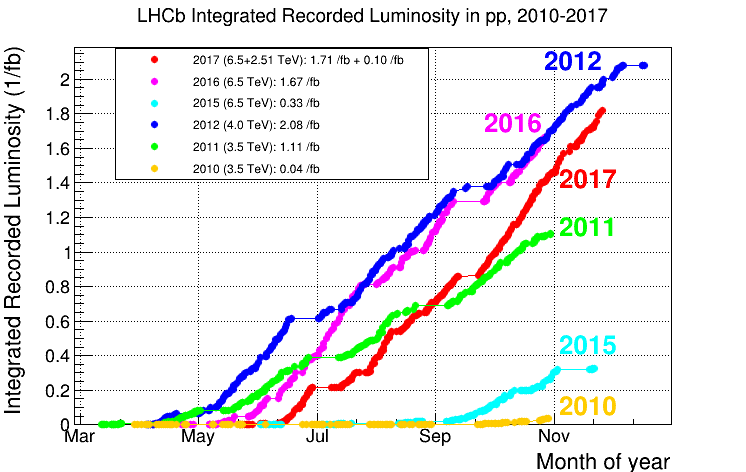
\includegraphics[width=0.9\textwidth]{02LHCb/figs/Luminosity.png}
  \end{center}
  \vspace{-2mm}
  \caption{Integrated luminosity of $pp$ collisions collected each year by LHCb.}
  \label{fig:luminosity}
\end{figure} 


\chapter{Flavour tagging}
\clearpage
%!TEX root = ../my_thesis.tex
\section{Flavour tagging algorithms}
\label{sec:tagging}

In this chapter, a description of the \emph{flavour tagging} techniques at LHCb is reported.
After a brief introduction to the methods,
the calibration of the \emph{Opposite Side} (OS) and \emph{Same Side} (SS) algorithms for the $\Bz\to\Dmp\pipm$ 
time-dependent analysis are 
described. Finally, a reoptimisation of the OS \emph{electron} (\OSe) tagger on both Run 1 and Run 2 data is reported. 
This work was made in collaboration with the University of Dortmund. During my PhD work
activity, I focused mainly on the OS calibration and OSe reoptimisation.

The identification of the flavour at production time of a neutral $B$ meson, \ie~whether it contained a $\bquark$ or a $\bquarkbar$ quark at
production, is a key element 
for any time-dependent analysis aiming at the measurement of oscillations and \CP~asymmetries, and in particular for the $\Bz\to
\Dpm\pimp$ analysis reported in this thesis. In fact, this information is needed in order to measure the decay rates or asymmetries introduced in Sec.~\ref{sec:Bphysics}.
Complications arise from two facts:
\begin{itemize}[noitemsep,topsep=0pt]
	\item neutral $B$ meson oscillate, so the flavour at the production time might differ from the flavour at the decay time;
	\item there are many final states, such as $\Dmp\pipm$, that can be produced by the decay of both $B$ and $\bar B$ mesons; so, the flavour cannot be obtained from the charge of the final state, even if there were no oscillations.
\end{itemize}
For these reasons, the flavour has to be reconstructed by exploiting particles not produced in the decay of the neutral $B$ meson being analysed.

Techniques to infer the initial flavour of a reconstructed
candidate are called flavour tagging algorithms.
Several flavour tagging algorithms exist in LHCb; they can be categorised into
same-side taggers (SS taggers) and opposite-side taggers (OS taggers). A
schematic representation of the taggers that can be used for tagging $\Bz$
mesons is shown in Fig.~\ref{fig:FTscheme}.
\begin{figure}[t]
	\begin{center}
		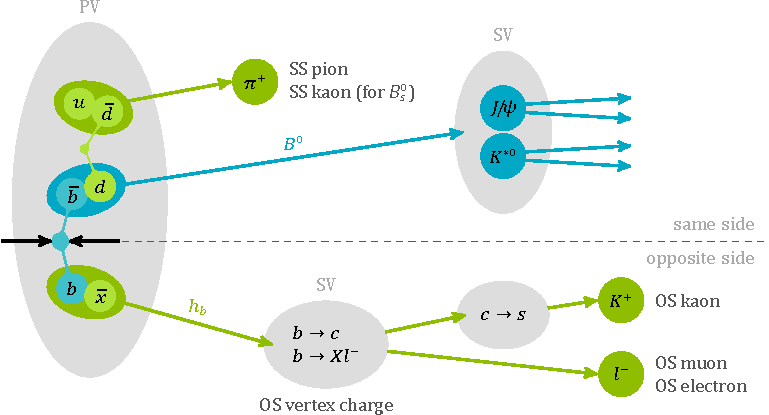
\includegraphics[width=0.8\textwidth]{04Flavourtagging/figs/FlavourTaggerScheme.pdf}
	\end{center}
        \vspace{-2mm}
	\caption{Flavour tagging algorithms used in LHCb. In this cartoon, the signal channel is considered to be $B^0\to J/\psi K^{*0}$.}
	\label{fig:FTscheme}
\end{figure}

The SS taggers infer the production flavour of the signal $\B$ meson by selecting
charged particle candidates that have a high chance of being remnants of the
hadronisation process of the $\B$ candidate
\cite{LHCb-PAPER-2016-039}. For $\Bz$ mesons, the same-side
pion tagger (\SSpi), which exploits charged $\pi$ mesons produced in the hadronisation of the
$\Bz$ meson, and the same-side proton tagger (\SSp), which looks for co-produced
protons, have been developed. For both taggers, the charge of the pion or proton is correlated with the production flavour of the signal $\Bz$ meson.
The response of the two taggers is combined into a
common SS response.

In contrast, the OS taggers exploit the predominant production process of $\B$
mesons via $\bbbar$ quark pair production \cite{LHCb-PAPER-2011-027}. They
partially reconstruct the decay of the \emph{other} $\bquark$ hadron produced along with each
reconstructed signal $\B$ meson, and infer its initial flavour. In fact, the flavour of the signal
$B$ meson and the other $\bquark$ hadron produced in the same collision are opposite.
Several OS taggers have been developed in LHCb, where the combination of the
OS kaon (\OSK), muon (\OSmu), electron (\OSe), and vertex charge (\OSvtx) tagging algorithms represents the
current standard OS combination. An additional OS tagger, the OS charm
tagger (\OSc)~\cite{LHCb-PAPER-2015-027}, can be exploited, and can be combined with
the OS standard combination.

Given a reconstructed candidate, each flavour tagging algorithm provides a
flavour tag $d$ and a prediction $\eta$ for the probability of the tag to be
wrong. This mistag probability $\eta$ is defined in the range $[0,0.5]$ and is
based on the output of multivariate classifiers, which are trained on datasets
of flavour-specific decays, and combine several kinematic and geometric
information on the tagging particle(s) and the event. The flavour tag takes the
values $d=+1$ for an initial $\Bz$, $d=-1$ for an initial $\Bzb$, and $d=0$ when
no tag could be assigned; this happens, for example, if the tagging particle fails 
the selection criteria of a given tagging algorithm, or if its trajectory lies outside
the detector acceptance.

More details on flavour tagging at LHCb can be found in
Refs.~\cite{Grabalosa:2012qra,LHCb-CONF-2011-003,LaThuile}.

%-------------------------------------------------------------------------------
\subsubsection{Performance characteristics}
\label{sec:tagging:characteristics}

The performance of flavour tagging algorithms can be characterised by different quantities. If $N_\mathrm{U}$ is the number of untagged
candidates and $N_\mathrm{W}$ ($N_\mathrm{R}$) is the number of wrongly (rightly) tagged candidates, the \emph{tagging efficiency}
(\ie~the fraction of tagged candidates) can be defined as
\begin{equation}
	\varepsilon_\text{tag}=\frac{N_\mathrm{R}+N_\mathrm{W}}{N_\mathrm{R}+N_\mathrm{W}+N_\mathrm{U}}.
	\label{eq:taggingefficiency}
\end{equation}
The fraction of wrongly tagged candidates, or \emph{mistag fraction}, is given by
\begin{equation}
\label{eq:mistag_def}
	\omega=\frac{N_\mathrm{W}}{N_\mathrm{R}+N_\mathrm{W}}.
\end{equation}
A non-zero mistag fraction dilutes the time-dependent asymmetries, reducing the experimental sensitivity to them. For instance, the measured decay rates for a $B\to f$ decay and its \CP-conjugate decay are
\begin{align}
	\frac{d\Gamma^{\rm meas}}{dt} &= (1-\omega)\frac{d\Gamma}{dt} + \omega \frac{d\bar\Gamma}{dt}, \\
	\frac{d\bar\Gamma^{\rm meas}}{dt} &= \omega\frac{d\Gamma}{dt} + (1-\omega) \frac{d\bar\Gamma}{dt}.
\end{align}
As a consequence, the measured \CP~asymmetry is
\begin{equation}
	A^{\rm meas}(t) = \frac{ \frac{d\bar\Gamma^{\rm meas}}{dt} - \frac{d\Gamma^{\rm meas}}{dt} }{ \frac{d\bar\Gamma^{\rm meas}}{dt} + \frac{d\Gamma^{\rm meas}}{dt} } 
	= \left(1-2\omega\right) \frac{ \frac{d\bar\Gamma}{dt} - \frac{d\Gamma}{dt} }{ \frac{d\bar\Gamma}{dt} + \frac{d\Gamma}{dt} } 
	= DA^{\rm phys}(t)\,, 
\end{equation}
where $A^{\rm phys}$ is the physical (true) \CP~asymmetry.
The quantity $D=1-2\omega$ is known as average \emph{dilution}. If $\omega=0$ (perfect tagger), then $D=1$ and no asymmetry dilution occurs. 
If $\omega=0.5$ (random tagger), then $D=0$, and it is not possible to measure the asymmetry anymore.

The quantity that can be interpreted as the figure of merit to
optimise a tagging algorithm is the
\emph{effective tagging efficiency}, also called \emph{tagging power}:
\begin{equation}
	\varepsilon_\text{eff}=\varepsilon_\text{tag}\left(1-2\omega\right)^2=\varepsilon_\text{tag}D^2.
\end{equation}
Assuming that $\varepsilon_\text{eff}$ is known without uncertainty, it can be shown that the statistical uncertainty on the physical asymmetry is given by
\begin{equation}
	\label{eq:sigma_on_asymm}
	\sigma_{A^{\rm phys}} = \frac{\sqrt{1-A^{\rm meas~2}}}{\sqrt{N\varepsilon_\text{tag}}\left(1-2\omega\right)}=\frac{\sqrt{1-A^{\rm meas~2}}}{\sqrt{N\varepsilon_\text{eff}}},
\end{equation}
where $N$ is the total number of candidates. So, according to Eq.~\ref{eq:sigma_on_asymm}, the greater the tagging power, the smaller the resulting statistical uncertainty on the \CP~asymmetry. 
Instead of using an average mistag fraction or \emph{probability} $\omega$, it is possible to exploit the
mistag probability $\eta$ estimated by the tagging algorithm. This probability $\eta$ is evaluated for each $B$ candidate individually, rather
than being a global quantity. Usually, $\eta$ needs to be \emph{calibrated} via a function $\omega(\eta)$ in order to return the true mistag probability (details in Sec.~\ref{sec:tagging:calibration}).
So, the tagging power can be rewritten as
\begin{equation}
	\label{eq:perevent_tagpower}
	\varepsilon_\text{eff} = \frac{1}{N}\sum_{i=1}^{N}D_i^2 = \frac{1}{N}\sum_{i=1}^{N}\left(1-2\omega(\eta_i)\right)^2,
\end{equation}
where $\omega(\eta_i)=0.5$ ($D_i=0$) for untagged candidates.

An example of dilution effect can be seen in Fig.~\ref{fig:dilution}, which shows how the measured amplitude of an asymmetry gets smaller for increasing values of $\eta$.

\begin{figure}[t]
	\begin{center}
		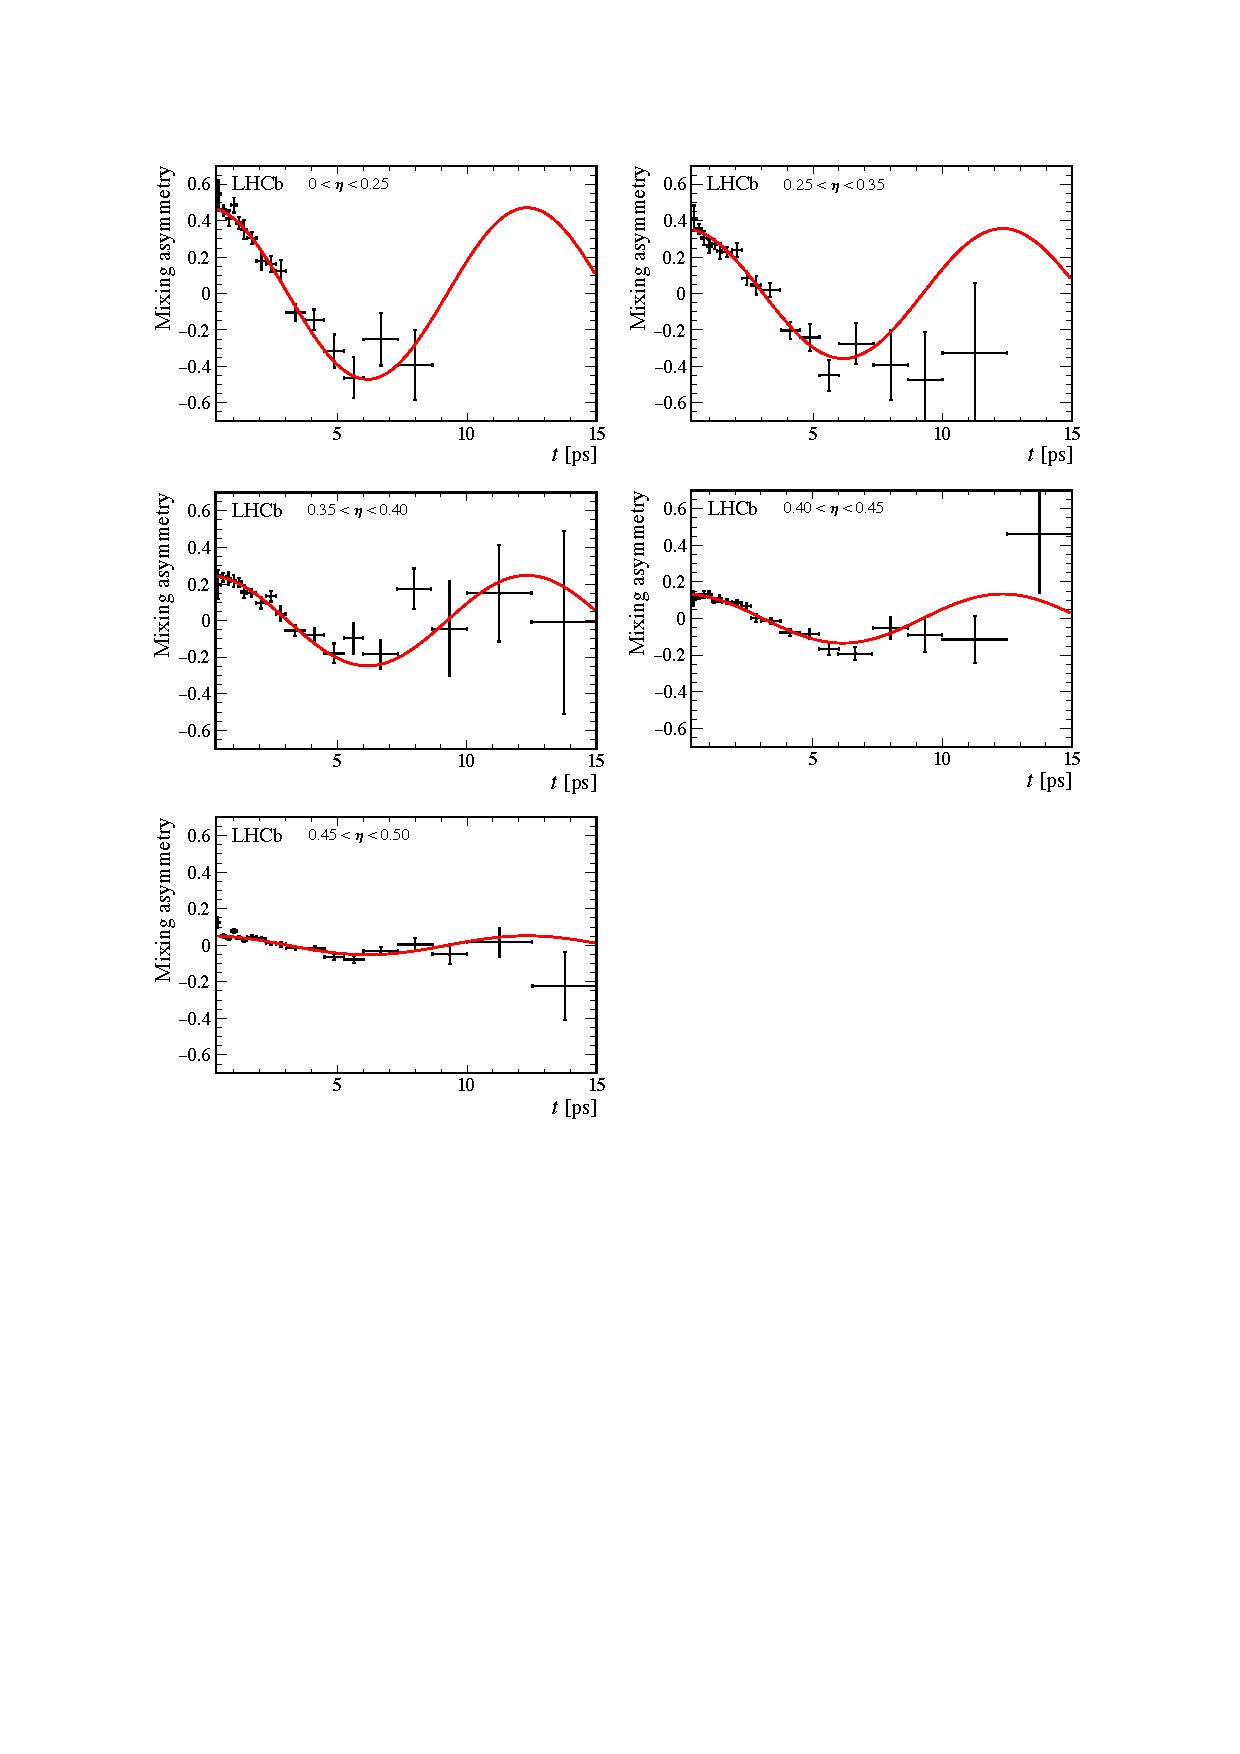
\includegraphics[width=0.9\textwidth]{04Flavourtagging/figs/Dilution.pdf}
	\end{center}
        \vspace{-2mm}
	\caption{Mixing asymmetry for SS-pion-tagged $\Bz\to\Dm\pip$ candidates in bins of increasing estimated mistag $\eta$~\cite{LHCb-PAPER-2016-039}.}
	\label{fig:dilution}
\end{figure}


%-------------------------------------------------------------------------------
\subsubsection{Calibration of the tagging output}
\label{sec:tagging:calibration}

The output of the flavour tagging algorithms is the result of training
multivariate classifiers (MVA) using datasets of flavour-specific $B$ decays, and
transforming the classifier output into mistag estimates $\eta$ through
regression. However, as the training and validation samples are different
from the signal sample used in the $\CP$ measurement (\eg~in terms of trigger
and selection criteria that affect the distribution of the MVA input features),
the output needs to be calibrated. Again, using control samples of flavour-specific decays, 
calibration functions $\omega(\eta)$ are obtained to
transform the mistag estimate $\eta$ of the algorithm to the mistag probability
$\omega$ measured in the control sample.

A common choice for the calibration function is a linear function:
\begin{equation}
	\omega(\eta)=p_0 + p_1\left(\eta-\langle\eta\rangle\right). \label{eq:FTcalibration}
\end{equation}
The use of the arithmetic mean $\langle\eta\rangle$ of the $\eta$ distribution
aims at a decorrelation of $p_0$ and $p_1$, hence a perfect calibration of the
taggers would result in $p_0=\langle\eta\rangle$ and $p_1=1$.

The performance of the flavour taggers is not necessarily independent of the
initial flavour of the \Bz. The charged decay products, like the \Kpm~mesons that are
used by the OS kaon tagger, can have significantly different interaction rates
with the detector material and therefore different reconstruction efficiencies.
This can result in different tagging efficiencies $\varepsilon_\text{tag}$ and
mistag probabilities $\omega$ for $\Bz$ and $\Bzb$. These tagging
asymmetries can dilute or enhance the observed raw asymmetry and need to be
corrected for. The asymmetries of the mistag probability, \ie~the difference of
the tagging calibration parameters $p_0$ and $p_1$ for initial $\Bz$ and $\Bzb$,
can be parameterised with two independent calibration functions:
\begin{equation}
	\begin{split}
          \label{eq:FTcalibrationSplit}
		\omega^{B^0}(\eta)  = p_0^{B^0}  + p_1^{B^0} \left(\eta-\langle\eta\rangle\right)\,,\\
		\omega^{\bar B^0}(\eta) = p_0^{\bar B^0} + p_1^{\bar B^0} \left(\eta-\langle\eta\rangle\right).
	\end{split}
\end{equation}
Equivalently, we can parameterise the calibration parameters $p_i$ (with $i=0,1$) as
\begin{equation}
	p_i^{B^0}=p_i+\frac{\Delta p_i}{2},\quad p_i^{\bar B^0}=p_i-\frac{\Delta p_i}{2}\,.
\end{equation}
The difference between the mistag of $\Bz$ and $\Bzb$ can be written as
\begin{equation}
		\Delta\omega(\eta)=\omega^{B^0}(\eta)-\omega^{\bar B^0}(\eta)=\Delta p_0+\Delta p_1\left(\eta-\langle\eta\rangle\right)\,.
\end{equation}

In this thesis, new models for the calibration functions are adopted instead
of the standard linear calibrations. These different parameterisations are
called \emph{Generalised Linear Models} (GLM), and are implemented in the EPM
(\emph{Espresso Performance Monitor}) package~\cite{EPM}. As will be explained in this section,
these models allow a great flexibility to cope with non-linearities, and solve technical issues
that may occur in fits that make use of flavour tagging. During my PhD, I worked
to refine some of these models and to include them in the fitting routines used for decay-time fits. 

In general, a GLM of order $N$ that relates the predicted mistag probability $\eta$ to the 
calibrated probability $\omega$ can be written as follows:
\begin{equation}
  \label{eq:glm_def}
  \omega(\eta) = g(h(\eta)) = g \left( g^{-1} (\eta) + \sum\limits_{i=1}^{N} \left(p_i + \frac{d\Delta p_i}{2}\right)f_i(\eta)\right)\,.
\end{equation}

The functions $f_i(\eta)$ are called \emph{basis functions}, and they can be chosen as polynomials or spline functions.
The set on basis functions is automatically orthogonalised by the EPM by using the Gram-Schmidt method~\cite{gram-schmidt}; this ensures that
the corresponding calibration parameters $p_i$ and $\Delta p_i$ are correlated as little as possible.

The parameter $d$ is the tagging decision, which is incorporated into the model in order to parameterise $\omega(\eta)$ for the two possible flavours.

The function $g$ is known as \emph{link function}. Usually, this is chosen as the inverse of a cumulative distribution
function in order to map input values into the interval $[0,1]$, such that the output can be naturally
interpreted as a probability.

For the $\Bz\to\Dpm\pimp$ analysis presented in this thesis, the adopted link function $g$ is a \emph{modified logistic function}, defined as
\begin{equation}
  \label{eq:rlogit}
  g(h) = \frac{1}{2(1+e^h)},
\end{equation}
where $h$ is defined in Eq.~\ref{eq:glm_def}. This link function is built such that the calibrated mistag probability
is defined in the interval $(0,0.5)$. This choice solves a numerical issue that often occurs when
standard link functions (\eg~identity or logistic) are adopted. In fact, if $\omega>0.5$, then an arbitrary
prescription has to be taken (\eg, label the candidate as untagged, or flip the tagging decision and take $1-\omega$ as
new calibrated mistag). If the calibration parameters are free in a time-dependent fit, this choice has to be made
during the minimisation process, according to the values $\omega$ takes at each iteration. This means that the relative
number of $B$ and $\bar B$, or the relative number of tagged and untagged candidates, may change during the fit, which
leads to numerical instabilities due to discontinuous changes in the likelihood function.

The EPM estimates the calibration parameters $p_i$ and $\Delta p_i$ via an unbinned maximum likelihood fit
called \emph{binomial regression}; this is an improvement over traditional, binned least-squares
fits, which are affected by a systematic uncertainty due to the binning choice.

%-------------------------------------------------------------------------------
\subsubsection{Combination of multiple taggers}
\label{sec:tagging:combination}

When more than one tagger is available per event, the tagging
decisions and mistag probabilities provided by each tagger can be combined into a single decision and a
single probability using the equations
\begin{equation}
	p(\bquark) = \prod_i\left(\frac{1}{2}-d_i\left(\frac{1}{2}-\eta_i\right)\right),\hspace{1cm}
	p(\bquarkbar) = \prod_i\left(\frac{1}{2}+d_i\left(\frac{1}{2}-\eta_i\right)\right), \label{eq:FTcombination1}
\end{equation}
where $p(\bquarkbar/\bquark)$ is the probability that the signal \Bz~contains a \bquarkbar/\bquark,
$d_i$ is the decision taken by the $i$-th tagger and
$\eta_i$ is the predicted mistag probability of the $i$-th tagger. These probabilities are
normalised as
\begin{equation}
	P(\bquarkbar) = \frac{p(\bquarkbar)}{p(\bquarkbar)+p(\bquark)}, \hspace{1cm} P(\bquark) = 1 - P(\bquarkbar). \label{eq:FTcombination2}
\end{equation}
If $P(\bquarkbar)>P(\bquark)$ the combined tagging decision is $d=+1$ and the final mistag probability is
$\eta = 1-P(\bquarkbar)$. Otherwise if $P(\bquark)>P(\bquarkbar)$ the combined tagging decision and the mistag
probability are $d=-1$ and $\eta=1-P(\bquark)$. 

Equation~\ref{eq:FTcombination1} is valid under the assumption that all taggers in the combination are independent.
In the $\Bz\to\Dmp\pipm$ analysis presented in this thesis, the OS taggers are combined in a single OS combination, and
the same is done for the SS taggers. Effects due to correlations among taggers within a combination are corrected for by calibrating
the combined predicted mistag.

%-------------------------------------------------------------------------------

\section[Flavour tagging strategy for the $\Bz\to\Dmp\pipm$ time-dependent analysis]{Flavour tagging strategy for the \boldmath{$\Bz\to\Dmp\pipm$} time-dependent analysis}
\label{sec:tagging:strategy}
In the $\Bz\to\Dpm\pimp$ analysis presented in this thesis, the OS combination (including the OS charm tagger) and the SS
combination are used. The implementation of the OS algorithms used in the combination are the same as described
in Refs.~\cite{LHCb-PAPER-2011-027,LHCb-PAPER-2015-027}; the OS algorithms other than the OS charm tagger were built as neural networks
trained on $\Bp\to J/\psi K^+$ Run 1 data, whereas the OS charm tagger was implemented with a BDT trained on a cocktail of simulated
$\Bp\to J/\psi K^+$, $\Bz\to\jpsi\Kstarz$ and $B^0_s\to J/\psi\phi$ decays.
The SS taggers have been reimplemented for this specific analysis by exploiting $\Bz\to\jpsi\Kstarz$ decays.
The functional form of the tagging calibrations is studied in control samples of
flavour-specific decays properly corrected to resemble the signal decay.
The calibration parameters are determined directly in the decay-time-dependent
fit of the signal described in Sec.~\ref{sec:datafit};
they are nuisance parameters of the likelihood function.
Determining the calibration parameters from the data along with
the \CP~observables is possible because the \CP~coefficients $C_f$ and $C_{\bar f}$ of Eqs.~\ref{eq:P0tof}--\ref{eq:P0bartofbar} are fixed in this analysis
(to \num{+1} and \num{-1} respectively). Hence, the cosine terms give sensitivity to the calibration parameters
independently of the sine terms, which are proportional to the $S_f$ and $S_{\bar{f}}$ coefficients. A heuristic explanation is presented in
Fig.~\ref{fig:amplitudes}.
\begin{figure}[t]
        \begin{center}
                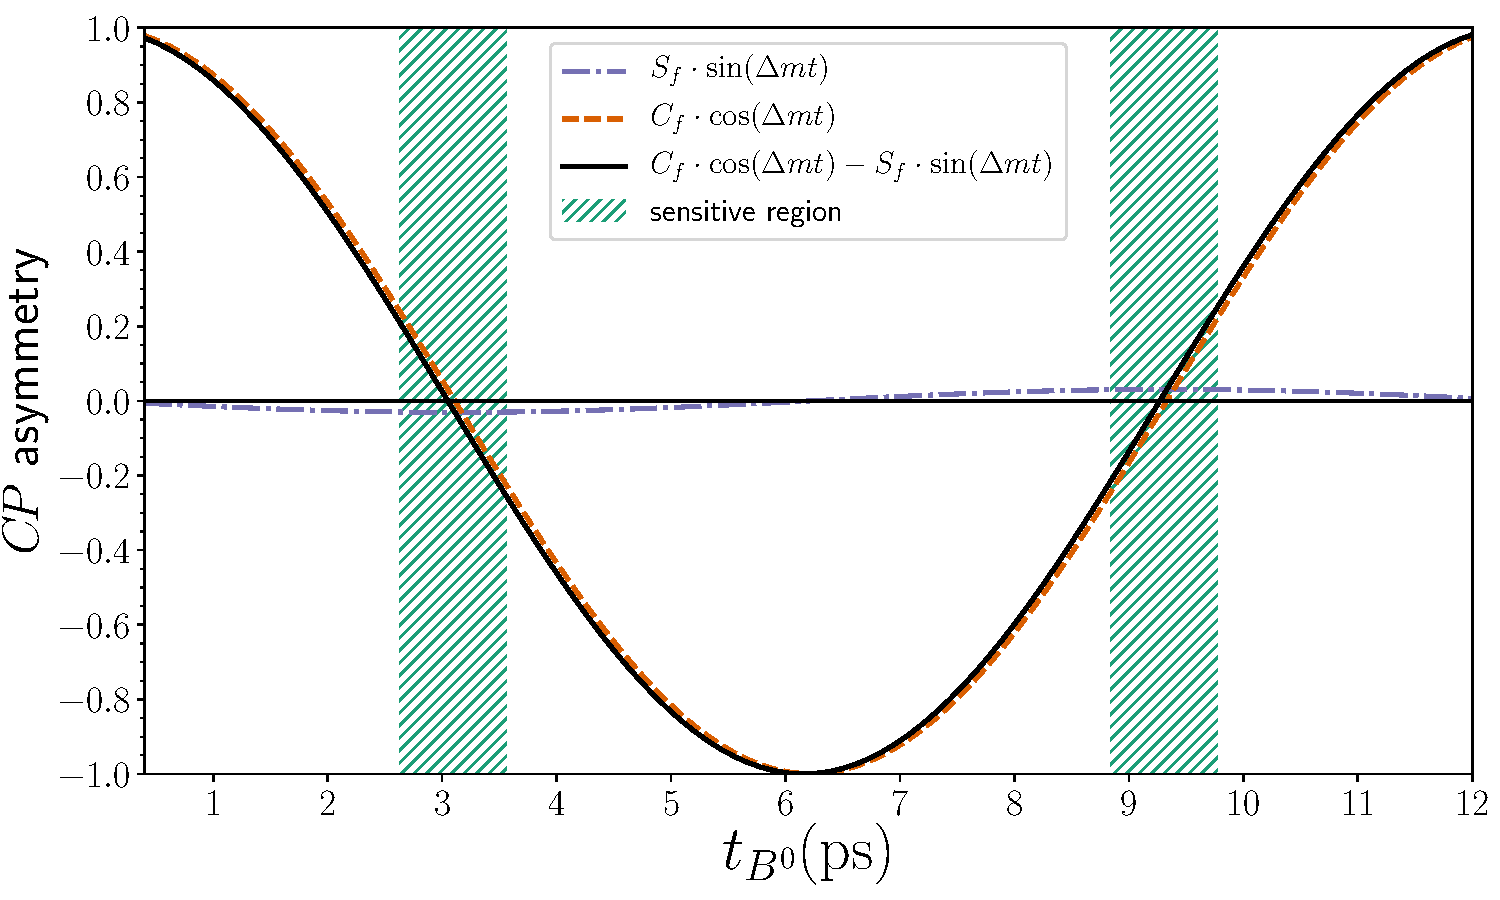
\includegraphics[width=0.48\linewidth]{04Flavourtagging/figs/oscillation_f.pdf}
                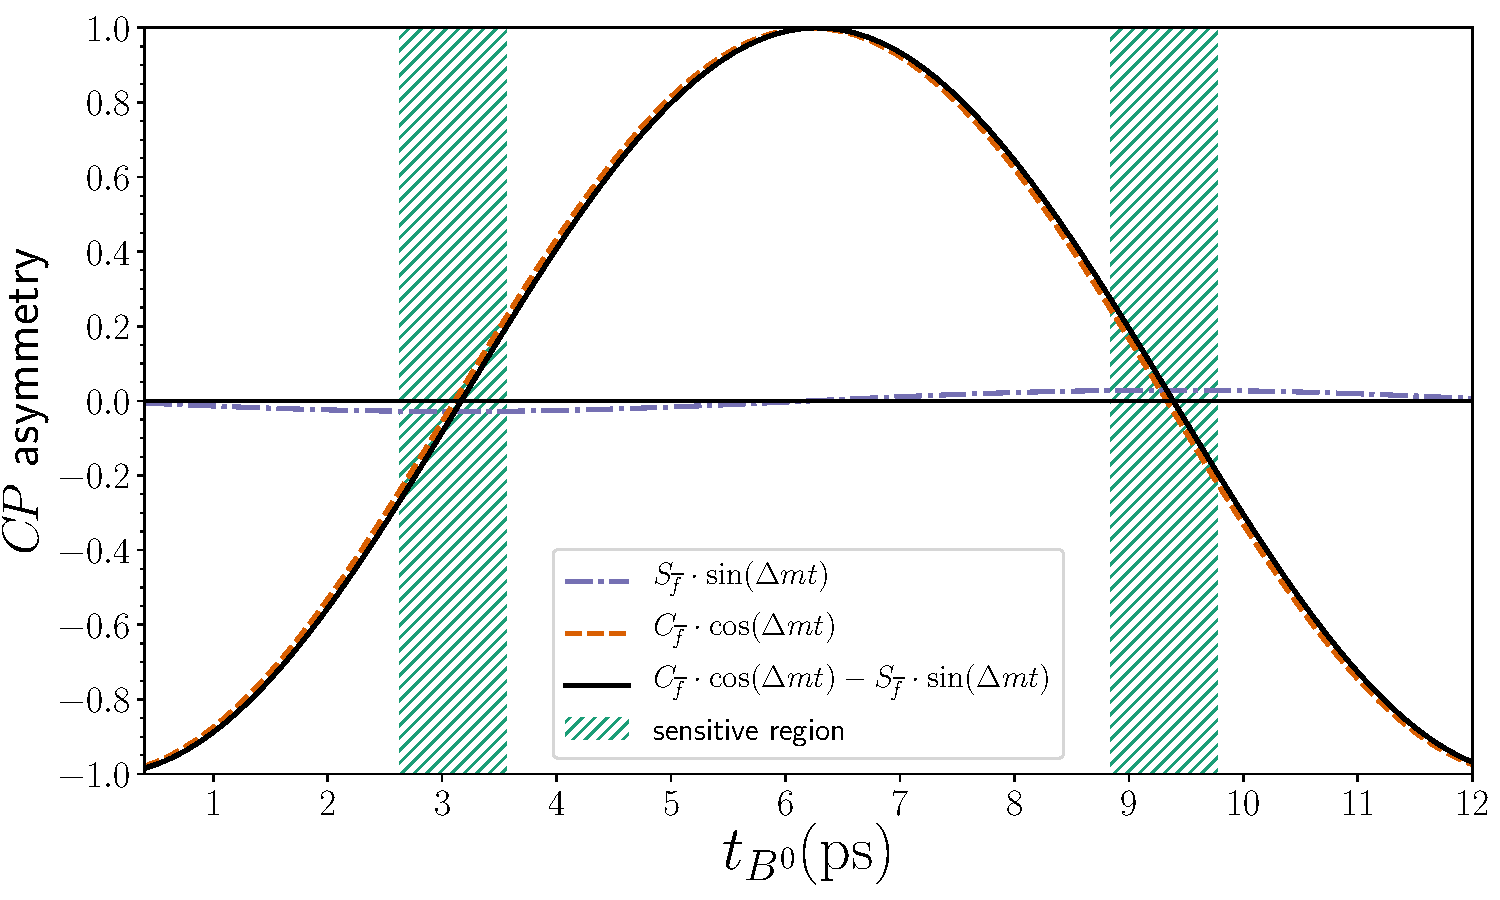
\includegraphics[width=0.48\linewidth]{04Flavourtagging/figs/oscillation_fbar.pdf}
        \end{center}
        \vspace{-2mm}
        \caption{$\bar\Bz$ versus $\Bz$ time-dependent asymmetries for the $\Dm\pip$ (left) and $\Dp\pim$
        (right) final states. The values of $C_f$, $C_{\bar f}$, $S_f$ and $S_{\bar f}$ are the ones used in simulation (see Appendix~\ref{app:mcgen}). 
        The sensitivity to $S_f$ and $S_{\bar f}$ is maximised in the
        intervals called ``sensitive regions'', since the $\sin(\Delta m)$ amplitude becomes of the same order of
        the $\cos(\Delta m)$ amplitude, which is close to zero. In the outer regions, since $C_f$ ($C_{\bar f}$) is
        fixed to $1$ ($-1$) in the fit, the mistag dilution (which depends on the flavour tagging calibration
        parameters) adapts to fit the $\cos(\Delta m)$ amplitude, giving sensitivity to the calibration parameters.}
        \label{fig:amplitudes}
\end{figure}
This strategy avoids any assumption on the portability
to the signal sample of the calibration parameters determined from the control
data. Such a strategy was studied extensively on simulation: the increase of the
statistical uncertainty of the $S_f$ and $S_{\bar{f}}$ coefficients given by the additional degrees of freedom of
the calibration parameters is smaller than the systematic
uncertainties associated with the calibration portability. Moreover,
the use of the calibration parameters from the control sample
causes biases on $S_f$ and $S_{\bar{f}}$ of the order of their statistical uncertainty; when letting
the calibration parameters float in the fit, such biases are suppressed or disappear, at the cost
of a moderate increase of the statistical uncertainty. In addition, while the precision
of the OS tagger calibration from the control sample is similar to the one from the
signal sample, the calibration of the SS tagger derived from the signal sample (Tab.~\ref{tab:timefitresult})
is much more precise than that from the control sample (Tab.~\ref{tab:calibrationSScombination}).

In what follows, the study of the tagging calibration from the control sample is presented.
For all reasons discussed above, these studies are not meant for determining the calibration parameters to use in
the time fit to the signal data (usual strategy adopted in all flavour-tagged time-dependent analyses), but they
serve the purpose of: i) determining the best functional form of the calibration functions to be used in the fit to
the signal; ii) having some reference values for the calibration parameters for a comparison with those extracted
from the signal.

The calibration for the OS combination are determined using $\Bp\to \Dzb\pip$ decays, as
described in Sec.~\ref{sec:tagging:OScalib}. The SS pion and the SS proton taggers were developed
using $\Bz\to\Dmp\pipm$ data and assuming negligible $\CP$ violation.
The use of these algorithms in this analysis could bias the measurement.
Therefore, the SS taggers are retrained using $\Bz\to\jpsi\Kstarz$ decays. The calibration of the SS
combination is described in Sec.~\ref{sec:tagging:SScalib}.

%===============================================================================
\subsection{Calibration of the opposite-side tagger combination}
\label{sec:tagging:OScalib}

\subsubsection{Data sample selection}
\label{sec:tagging:OScalib:selection}

The calibration parameters of the OS tagger combination (namely the combination of
the OS electron, muon, kaon, vertex charge, and charm algorithms) are determined using $\Bp\to
\Dzb(\to \Kp\pim)\pip$ candidates reconstructed in $3\invfb$ of data.
Such a control decay mode provides very high statistics (more than 300k OS-tagged signal candidates) and
is very similar to the signal decay $\Bz\to\Dm\pip$.

Candidate $\Bp\to\Dzb\pip$ decays are selected through the \spverb!B2D0PiD2HHBeauty2CharmLine! stripping line,
versions \spverb!S21r1! (2011 data) and \spverb!S21! (2012 data), of the \spverb!BhadronCompleteEvent! stream.
The $\Bp$ candidates are required to be TOS, \ie~to trigger on \\
\spverb!Hlt1TrackAllL0Decision! at the HLT1 stage,
and at least one among \\
\path{Hlt2Topo2BodyBBDTDecision},
\path{Hlt2Topo3BodyBBDTDecision}, and \\
\path{Hlt2Topo4BodyBBDTDecision} at HLT2.
The additional requirements listed in Table~\ref{tab:OSSelection} are applied to further
suppress backgrounds and enhance the signal purity.

A fit to the mass distribution of $\Bp$ candidates is done to calculate \emph{sWeights},
used in the subsequent steps of the analysis to subtract the backgrounds surviving the selection.
This fit is described in details in Appendix~\ref{app:OSmassFit}.

Event-by-event weights are calculated to equalise the $\Bp\to\Dzb\pip$ and $\Bz\to\Dmp\pipm$ distributions of the variables on which
the tagging calibration can depend. The procedure and the results of this reweighting are reported in
Appendix~\ref{app:ReweightingOSTagging}. Additionally, the number of \Bp and \Bm candidates are made equal in the sample to avoid any spoil of the calibration
parameters due to a \Bp/\Bm production asymmetry or a detection asymmetry.
All these weights, along with \emph{sWeights}~\cite{Pivk:2004ty}, are applied during
the calibration procedure.

\begin{table}[htbp]
	\centering
	\caption{Selection requirements for the $\Bp\to\Dzb\pip$ candidates.}
	\begin{tabular}{ccc}
		\toprule
		Description & Variable & Requirement \\
		\midrule
		\multicolumn{3}{c}{Bachelor track } \\
		\midrule
		muon identification criteria & $\text{IsMuon}$ & $=0$ \\
		ghost probability & $p_\text{ghost}$ & $<0.1$ \\
		quality of track & $\chi^2_\text{track}/\text{ndof}$ & $<2$ \\
		\midrule
		\multicolumn{3}{c}{$\Dz$ daughter tracks} \\
		\midrule
		$\ln L_K - \ln L_\pi$ & $\text{PIDK}$ & $>-2$ (kaon), $<8$ (pion) \\
		ghost probability & $p_\text{ghost}$ & $<0.1$ \\
		quality of track & $\chi^2_\text{track}/\text{ndof}$ & $<2.5$ \\
		\midrule
		\multicolumn{3}{c}{$\Dz$ candidate} \\
		\midrule
		invariant mass & $m_{K\pi}$ & $m_{K\pi}\in [1830,1904]~\mevcc$ \\	
		\midrule
                \multicolumn{3}{c}{$\Bp$ candidate} \\
		\midrule
		decay time & $\tau_{\Bp}$ & $\tau_{\Bp}\in [0.2,15]~\rm ps$ \\
		minimum IP $\chi^2$ w.r.t. PV & $\text{MIN}\chi^2\text{IP}_\text{PV}$ & $<15$ \\
		\bottomrule
	\end{tabular}
	\label{tab:OSSelection}
\end{table}

\subsubsection{Calibration}
\label{sec:tagging:OScalib:calibration}
The calibration of the estimated mistag $\eta$ is performed on the fully reweighted $\Bp\to\Dzb\pip$ dataset. 
A GLM model with NSpline basis function~\cite{EPM} is adopted.
The projection of the fitted calibration function over the $\Bp\to\Dzb\pip$ dataset is shown in Fig.~\ref{fig:oscalibplot},
whereas the fitted calibration parameters are listed in Table~\ref{tab:oscalibparams}.
\begin{figure}[htbp]
        \begin{center}
                \includegraphics[width=0.80\textwidth]{04Flavourtagging/figs/OS_Combination_Calibration_Data.png}
        \end{center}
        \vspace{-5mm}
        \caption{Mistag $\omega$ measured in bins of predicted mistag $\eta$ for reweighted $\Bp\to\Dzb\pip$ candidates (data points) and fitted calibration function. The green (yellow) band indicates the $68\%$ ($95\%$) confidence interval on the calibration function.}
        \label{fig:oscalibplot}
\end{figure}
\begin{table}[htbp]
        \centering
        \caption{Fitted OS calibration parameters on the $\Bp\to\Dzb\pip$ reweighted dataset.}
        \begin{tabular}{cc}
                \toprule
                Parameter & Fitted value \\
                \midrule
                $p_0$ & $-0.136 \pm 0.019$\\
                $p_1$ & $-0.006 \pm 0.022$\\
                $p_2$ & $-0.0107 \pm 0.0083$\\
                $p_3$ & $-0.5 \pm 0.10$\\
                $p_4$ & $-0.85 \pm 0.46$\\
                $\Delta p_0$ & $-0.129 \pm 0.038$\\
                $\Delta p_1$ & $0.042 \pm 0.045$\\
                $\Delta p_2$ & $-0.020 \pm 0.017$\\
                $\Delta p_3$ & $0.42 \pm 0.21$\\
                $\Delta p_4$ & $1.91 \pm 0.92$\\
                \bottomrule
        \end{tabular}
        \label{tab:oscalibparams}
\end{table}
The number of free parameters in the adopted GLM model (10) has been chosen in order to have  
satisfactory goodness-of-fit (GOF) metrics (details in Appendix~\ref{app:chooseOSdegree}).

\subsubsection{Calibration portability}
\label{sec:tagging:OScalib:portability}

The aim of the calibration is to return a mistag $\omega$ as close as possible to the \emph{true} mistag, which would
be given by a \emph{true calibration}. The latter is not defined for $\Bz\to\Dm\pip$ decays in data, but it is possible to estimate it 
for $\Bz\to\Dm\pip$ decays on MC. In fact, since the true flavour of the $\Bz$ meson
is known in MC, this true MC calibration can be done in the same way as $\Bp\to\Dzb\pip$, where the true flavour is given by the $B$ charge.

This $\Bz\to\Dm\pip$ calibration is performed after equalising the number of $\Bz$ and $\bar\Bz$ in the sample, in order to disentangle
tagging asymmetries from \CP~violation and production asymmetries.

The $\Bp\to\Dzb\pip$ MC calibration is performed in exactly the same way as described in Sec.~\ref{sec:tagging:OScalib:calibration}, except that no
\emph{sWeights} are considered, since only true MC signal decays are used.

The two calibrations using the $\Bz\to\Dm\pip$ and $\Bp\to\Dzb\pip$ MC samples are shown in Fig.~\ref{fig:os_calib_portability_mc} and compared in Table~\ref{tab:os_calib_portability_mc}. A more robust comparison is obtained from a $\chi^2$ function describing the discrepancy between the two calibrations by taking the covariance matrices into account. The overall discrepancy (corresponding to the $\chi^2$ minimum) is around $2~\sigma$.

\begin{figure}[t!]
        \begin{center}
                \includegraphics[width=0.45\textwidth]{04Flavourtagging/figs/OS_Combination_Calibration_Bu_MC.png}
                \includegraphics[width=0.45\textwidth]{04Flavourtagging/figs/OS_Combination_Calibration_Bd_MC.png}
        \end{center}
        \vspace{-5mm}
        \caption{Mistag $\omega$ measured in bins of predicted mistag $\eta$ for reweighted $\Bp\to\Dzb\pip$ (left) and $\Bz\to\Dm\pip$ (right) candidates (data points) and fitted calibration functions. The green (yellow) band indicates the $68\%$ ($95\%$) confidence interval on the calibration functions.}
        \label{fig:os_calib_portability_mc}
\end{figure}

\begin{table}[t!]
        \centering
        \caption{Comparison between the fitted OS tagging calibration parameters using truth-matched $\Bp\to\Dzb\pip$ and $\Bz\to\Dm\pip$ MC decays. The discrepancy in each parameter is computed assuming independent datasets.}
        \begin{tabular}{cccc}
          \toprule
          Parameter   &  $\Bp\to\Dz\pip$   &  $\Bz\to\Dm\pip$  &   Discrepancy ($\sigma$) \\
          \midrule
          $p_0$   &   $-0.065\pm0.011$   &   $-0.0996\pm0.0066$   &   $2.70$ \\
          $p_1$   &   $-0.190\pm0.012$   &   $-0.1492\pm0.0077$   &   $-2.84$ \\
          $p_2$   &   $-0.0105\pm0.0044$   &   $-0.0191\pm0.0029$   &   $1.63$ \\
          $p_3$   &   $-0.295\pm0.054$   &   $-0.234\pm0.036$   &   $-0.93$ \\
          $p_4$   &   $-0.42\pm0.26$   &   $-0.14\pm0.20$   &   $-0.85$ \\
          $\Delta p_0$   &   $-0.059\pm0.022$   &   $-0.058\pm0.013$   &   $-0.03$ \\
          $\Delta p_1$   &   $0.044\pm0.024$   &   $0.030\pm0.015$   &   $0.46$ \\
          $\Delta p_2$   &   $-0.0012\pm0.0088$   &   $-0.0126\pm0.0058$   &   $1.08$ \\
          $\Delta p_3$   &   $-0.08\pm0.11$   &   $-0.046\pm0.073$   &   $-0.25$ \\
          $\Delta p_4$   &   $-0.34\pm0.53$   &   $-0.29\pm0.39$   &   $-0.08$ \\
          \bottomrule
        \end{tabular}
        \label{tab:os_calib_portability_mc}
\end{table}

%===============================================================================
\subsection{Calibration of the same-side tagger combination}
\label{sec:tagging:SScalib}

As described in Ref.~\cite{LHCb-PAPER-2016-039}, the SS pion and proton taggers
were both trained on the $\num{2012}$ data sample of
$\Bz\to\Dmp\pipm$ decays. As the effect of $\CP$ violation was neglected during the
training the algorithms and the underlying MVAs cannot be blindly used when
measuring $\CP$ violation in the same decay channel. Thus, $\Bz\to\jpsi\Kstarz$
decays are chosen instead, as they represent a flavour-specific $\Bz$ decay with
a large signal yield of about $350000$ candidates in 2012 data. 

Once the SS pion and proton taggers are implemented, they are combined into
a single SS combination as described in Sec.~\ref{sec:tagging:combination}.

%-------------------------------------------------------------------------------
\subsubsection{Calibration}
\label{sec:tagging:SScalib:combo}

The calibration is performed on a $\Bz\to\jpsi\Kstarz$ data subsample that is not used for the SS pion and proton training.
A GLM model having a first order polynomial is chosen as basis function and a
modified logistic function (Eq.~\ref{eq:rlogit}) is used as link. The number of free parameters in this model (4) is tuned in order to have
satisfactory goodness-of-fit (GOF) metrics. Together with the \emph{sWeights},
additional weights to correct the $\Bz\to\jpsi\Kstarz$ data to resemble the $\Bz\to\Dmp\pipm$ data are applied during the calibration. The
resulting calibration parameters are listed in Table~\ref{tab:calibrationSScombination} and a graphical representation of the calibration 
is presented in Fig.~\ref{fig:calibrationSScombination}.
\begin{table}[tbp]
	\centering
	\caption{Fitted SS calibration parameters obtained on the $\Bz\to\jpsi\Kstarz$ data sample (calibration
	subsample).}
	\begin{tabular}{cccc}
		\toprule
		$p_0$ & $p_1$ & $\Delta p_0$ & $\Delta p_1$ \\
		\midrule
		\num{-0.091\pm0.059}  & \num{-0.027\pm0.065} & \num{0.034\pm0.084} &\num{0.032\pm0.094}\\
		\bottomrule
	\end{tabular}
	\label{tab:calibrationSScombination}
\end{table}
\begin{figure}[tbp]
	\begin{center}
		\includegraphics[width=0.80\textwidth]{04Flavourtagging/figs/SScalib.png}
	\end{center}
        \vspace{-2mm}
	\caption{Mistag $\omega$ measured in bins of predicted mistag $\eta$ for reweighted $\Bz\to\jpsi\Kstarz$ candidates (data points) and fitted calibration function. The green (yellow) band indicates the $68\%$ ($95\%$) confidence interval on the calibration function.}	
	\label{fig:calibrationSScombination}
\end{figure}
%-------------------------------------------------------------------------------
\subsubsection{Calibration portability}
\label{sec:tagging:SScalib:portability}

In the same way as for the OS taggers (Sec.~\ref{sec:tagging:OScalib:portability}), the portability of the SS tagging calibration is checked on Monte Carlo. 
For $\Bz\to\Dm\pip$ the calibration is performed using the true flavour of the $\Bz$ meson after
equalising the number of $\Bz$ and $\bar\Bz$ in the sample, in order to disentangle tagging asymmetries from \CP~violation
and production asymmetries. Also on $\Bz\to\jpsi\Kstarz$ the true flavour of the $\Bz$ meson is used for the calibration, and
no \emph{sWeights} are needed, since only the true MC signal decays are used.

The two calibrations using the  $\Bz\to\Dm\pip$ and $\Bz\to\jpsi\Kstarz$ Monte Carlo samples are shown in
Fig.~\ref{fig:ss_calib_portability_mc} and compared in
Table~\ref{tab:ss_calib_portability_mc}. A full comparison that takes into account the correlation between the
parameters is obtained from a $\chi^2$ test similar to the one described in Sec.~\ref{sec:tagging:OScalib:portability}. The agreement is around \SI{0.1}{\sigma}. Even thought this test doesn't hint to
issues of portability between the decay modes, the same strategy used for the OS calibrations is followed, i.e fitting the
parameter directly in data with the \CP~asymmetries. This is motivated by the fact that 
the $\Bz\to\Dm\pip$ signal sample has much more sensitivity to determine the
parameters than the $\Bz\to\jpsi\Kstarz$ sample. In addition, with this approach no systematic related to calibration
portability is necessary, consistent with the OS tagger treatment.

\begin{figure}[t]
        \begin{center}
                \includegraphics[width=0.45\textwidth]{04Flavourtagging/figs/SS_Combination_Calibration_BdJpsiKst_MC.png}
                \includegraphics[width=0.45\textwidth]{04Flavourtagging/figs/SS_Combination_Calibration_BdDpi_MC.png}
        \end{center}
        \vspace{-2mm}
        \caption{Mistag $\omega$ measured in bins of predicted mistag $\eta$ for reweighted $\Bz\to\jpsi\Kstarz$ (left) and $\Bz\to\Dm\pip$ (right) candidates (data points) and fitted calibration functions. The green (yellow) band indicates the $68\%$ ($95\%$) confidence interval on the calibration functions.}
        \label{fig:ss_calib_portability_mc}
\end{figure}

\begin{table}[tbp]
        \centering
        \caption{Comparison between the fitted SS tagging calibration parameters using truth-matched \mbox{$\Bz\to\jpsi\Kstarz$} and $\Bz\to\Dm\pip$
        MC decays. The discrepancy in each parameter is computed assuming independent datasets.}
        \begin{tabular}{cccc}
          \toprule
          Parameter   &  $\Bz\to\jpsi\Kstarz$   &  $\Bz\to\Dm\pip$  &   Discrepancy ($\sigma$) \\
          \midrule
          $p_0$   &   $-0.016\pm0.017$   &   $-0.019\pm0.008$   &   $-0.19$ \\
          $p_1$   &   $0.063\pm0.021$   &   $0.060\pm0.010$   &   $-0.14$ \\
          $\Delta p_0$   &   $-0.029\pm0.033$   &   $-0.027\pm0.015$   &   $0.04$ \\
          $\Delta p_1$   &   $-0.026\pm0.041$   &   $0.015\pm0.019$   &   $0.90$ \\
          \bottomrule
        \end{tabular}
        \label{tab:ss_calib_portability_mc}
\end{table}

%===============================================================================
%!TEX root = ../my_thesis.tex
\section{Optimisation of the opposite-side electron tagger}
\label{sec:tagging:OSeOpt}

%%%%%%%%%%%%%%%%%%%%%%%%%%%%%%%%%%%%%%%%%%%%%%%%%%%%

The performance of the flavour tagging algorithms depends on the data taking conditions, in particular the centre-of-mass energy
of the $pp$ collision. 

On one hand, the tagging power of the SS taggers shows an increase on Run 2 data as compared to Run 1, thanks to either a higher tagging efficiency (\SSpi~and \SSp) or a lower mistag rate (\SSK). This is due to the higher boost of the $b\bar b$ quark pair at $13~\rm TeV$, which makes the momentum spectrum of $B$ mesons and fragmentation tracks harder, and increases the acceptance of the fragmentation tracks. 

On the other hand, the tagging power of the existing \OSe, \OSmu, and \OSK~taggers decreases on Run 2 data. The reason for this degradation is mainly due to the higher track multiplicity, which increases the probability to have a wrong tag decision. Moreover, because of the different Run 2 kinematics, the criteria to select the tagging particles are no longer optimal, thus giving a lower tagging efficiency.

The performance of the \OSc~and~\OSvtx~algorithms is, on average, compatible or better on Run 2 as compared to Run 1.

In this section, the reoptimisation of the \OSe~tagger is presented. This reoptimisation is performed both on Run 2 data, in order to recover the observed loss in tagging power, and on Run 1 data, to further improve the already existing algorithm.
This reoptimisation consists of two main steps. First, selection criteria are applied to select electron-like particles, yielding a sample of $B$ signal candidates with a low average tagging power. Then, a BDT classifier is applied to discriminate between $B$ candidates with right and wrong tag decisions for each selected track. Finally, for each $B$ candidate, the BDT output for the track with the highest transverse momentum is converted into a predicted mistag probability. 

A similar approach is followed for the development of the \OSK~and \OSmu~taggers. In this case, the reoptimisation on Run 1 data does not show any gain in performance, whereas some significant gain is found on Run 2 data.

%%%%%%%%%%%%%%%%%%%%%%%%%%%%%%%%%%%%%%%%%%%%%%%%%%%%

\subsection{Sample definition}

The \OSe~algorithm is developed in a data-driven fashion by using \emph{sWeighted} samples of $B^+\to J/\psi K^+$ decays. The full Run 1 dataset (2011+2012) is used to optimise the algorithm on Run 1 conditions, whereas the 2016 dataset is exploited to optimise the tagger on Run 2 conditions. An alternative optimisation on \emph{sWeighted} 2016 $B^+\to \Dzb \pi^+$ data is performed in parallel. The motivation for this is to cross-check the Run 2 implementation with an independent decay mode, which is characterised by different kinematics than that of $B^+\to J/\psi K^+$.
Hereafter, the \OSe~tagger optimised on Run 1 $B^+\to J/\psi K^+$ data will be indicated as ``Run 1 new'' version, in order to distinguish it from the previous ``Run 1 old'' version introduced in Ref.~\cite{LHCb-PAPER-2011-027}, which was based on simple selection criteria and a neural network for the mistag estimation.  
The \OSe~tagger optimised on Run 2 $B^+\to J/\psi K^+$ and $B^+\to \Dzb \pi^+$ data will be denoted as ``Run 2 B2CC'' and ``Run 2 B2OC'' versions, respectively.
Moreover, it is understood that the tunings of all the PROBNN features mentioned in this section are \texttt{MC12TuneV2} for Run 1 data and \texttt{MC15TuneV1} for Run 2 data.

Each dataset is divided in four subsamples:
\begin{itemize}[noitemsep,topsep=0pt]
  \item the first subset, including $\sim 25~\%$ of the total data, is used for the optimisation of the electron preselection (Sec.~\ref{sec:tagging:OSePresel});
    \item the second subset (\emph{training sample}), including $\sim 50~\%$ of the total data, is adopted as training set for the BDT classifier used for\
 the predicted mistag estimation (Sec.~\ref{sec:tagging:OSeBDT}). This sample is also used for tuning some \emph{hyperparameters} (number of trees, maximum depth) which define the BDT classifier.
 \item the third and the fourth subsets (\emph{evaluation set 1} and \emph{2}), each including $\sim 12.5~\%$ of the total data, are adopted together \
as test sets to check for overtraining (Sec.~\ref{sec:tagging:OSePerf1}). The evaluation set 1 is also used to calibrate the obtained tagger, which is then applied to the second evaluation set in order to measure the performance; the procedure is then repeated by swapping the two samples (\emph{two-fold validation}).
\end{itemize}

%%%%%%%%%%%%%%%%%%%%%%%%%%%%%%%%%%%%%%%%%%%%%%%%%%%%

\subsection{Preselection optimisation}
\label{sec:tagging:OSePresel}

Electron-like particles are selected by means of a set of requirements. The reconstructed tracks must not be associated to
the $B$ signal decay tree,
and must not have hits in the muon detector in order to exclude muons (already exploited by the \OSmu~algorithm).
Moreover, these tracks have to be of type long, lie in the ECAL acceptance, and have sufficient reconstruction quality ($\chi^2/\rm ndof<3$). 
Also, the inverse of the rigidity $e/p$ has to be comprised between 0.85 and 2, and the charge deposited in the VELO detector must be
smaller than 1.4 normalised Analogic-to-Digital Converter (ADC) counts.
Finally, tracks where the fit for the track IP with respect to the primary vertex did not converge are excluded. 

A further selection is applied in order to enhance the average tagging power of the resulting sample, which is defined as
\begin{equation}
        \label{eq:avgtagpower}
        \avg{\effeff} = \varepsilon_\text{tag} \left[1 - 2 \frac{\sum\limits_{i=1}^N w_i f^i_{\rm R}}{\sum\limits_{i=1}^N w_i (f^i_{\rm R} + f^i_{\rm W})}\right]^2,
\end{equation}
where $w_i$ are the \emph{sWeights}, while $f^i_{\rm R}$ ($f^i_{\rm W}$) is the fraction of particles giving the right (wrong) flavour for the $i$th $B$ candidate, with $f^i_{\rm R}+f^i_{\rm W}=1$ for every candidate.

The expression of Eq.~\ref{eq:avgtagpower} is taken as the figure of merit to maximise during the selection optimisation. This maximisation is performed numerically by using gradient boosted regression trees to model $\avg{\effeff}$ as a function of the applied cuts~\cite{scikit-optimize}. The cuts are optimised separately for the Run 1 new, Run 2 B2CC and Run 2 B2OC algorithms; in all cases, about $25\%$ of the available data for each sample is used. 

The resulting, optimised requirements are reported in Table~\ref{tab:OSegbselection}, while the convergence plots of the minimisation are shown in Fig.~\ref{fig:OSegbconvergence}.

After the optimisation, the performance of the selection (including the average tagging power defined in Eq.~\ref{eq:avgtagpower}) is evaluated on the remaining $75\%$ of data for each sample, yielding the results shown in Table~\ref{tab:OSegbperformance}.

\begin{table}
	\centering
        \caption{Optimised requirements for the preselection of tracks used by the \OSe~algorithm.
          $p_{\rm ghost}$ is the probability for the track to be a fake combination of hits.
          IPPU denotes the impact parameter with respect to the pile-up vertex in the event, which might be
        reconstructed in the event in addition to the nominal PV.
        $\Delta\phi$ is the difference in azimuthal angle between the track and the signal $B$ candidate.}
         \label{tab:OSegbselection}
        \begin{tabular}{llll}
        \toprule
        Requirement & Run 1 new & Run 2 B2CC & Run 2 B2OC \\
        \midrule
        $p_{\rm ghost}<$ & $0.861$ & $0.843$ & $0.348$ \\
        PROBNN$\pi<$ & $0.934$ & $0.983$ & $0.980$ \\
        PROBNN$p<$ & $0.719$ & $0.271$ & $0.732$\\
        PROBNN$K<$ & $0.765$ & $0.695$ & $0.954$\\
        PROBNN$e>$ & $0.061$ & $0.243$ & $0.040$\\
        PROBNN$\mu<$ & $0.938$ & $0.158$ & $0.263$ \\
        PID$e>$ & $4.555$ & $4.333$ & $-0.691$\\
        $p_{\rm T}>$ (\mevc) & $1132$ & $1403$ & $1263$ \\
        $p>$ (\mev) & $3114$ & $5035$ & $2246$\\
        $\sigma_{\rm IP}/\rm IP>$ & $0.020$ & $0.042$ & $1.410$ \\
        $\sigma_{\rm IPPU}/\rm IPPU>$ & $12.101$ & $9.335$ & $2.758$ \\
        min $\Delta\phi>$ & $0.00803$ & $0.0167$ & $0.0299$\\   
        \bottomrule
        \end{tabular}
\end{table}

\begin{table}
	\centering
        \caption{Performance of the preselection (\OSe~algorithm) applied on the data not used for the preselection optimisation ($\sim 75\%$ of the total dataset for each sample). The average tagging power $\avg{\effeff}$ is defined in Eq.~\ref{eq:avgtagpower}.}
        \label{tab:OSegbperformance}
        \begin{tabular}{llll}
        \toprule
        Algorithm & $\etag$ (\%) & $\avg{\mistag}$ (\%) & $\avg{\effeff}$ (\%) \\
        \midrule
        Run 1 new & $3.440\pm0.019$ & $33.31\pm0.27$ & $0.383\pm0.007$ \\
        Run 2 B2CC & $2.514\pm0.017$ & $33.50\pm0.32$ & $0.274\pm0.006$ \\
        Run 2 B2OC & $3.664\pm0.024$ & $34.32\pm0.32$ & $0.360\pm0.006$ \\
        \bottomrule
        \end{tabular}
\end{table}

\begin{figure}[htbp]
	\begin{center}
        \includegraphics[width=0.4\textwidth]{04Flavourtagging/figs/OSelectronOpt/2017-12-12-vibattis-OSElectron-tagpartseloptimisation_Run1/ConvergenceOSe2017-nominal.pdf}
        \includegraphics[width=0.4\textwidth]{04Flavourtagging/figs/OSelectronOpt/2017-12-12-vibattis-OSElectron-tagpartseloptimisation_Run2/ConvergenceOSe2017-nominal.pdf} \\
        \includegraphics[width=0.4\textwidth]{04Flavourtagging/figs/OSelectronOpt/2018-04-06-vibattis-OSElectron-tagpartseloptimisation_Run2_Bu2D0pi/ConvergenceOSe2017-nominal.pdf} \\
       \end{center}
        \vspace{-2mm}
        \caption{Maximised value of the average tagging power as a function of the gradient boosted regression tree algorithm iteration for the Run 1 new (top left), Run 2 B2CC (top right) and Run 2 B2OC (bottom) implementations of the \OSe~tagger.}
        \label{fig:OSegbconvergence}
\end{figure}

%%%%%%%%%%%%%%%%%%%%%%%%%%%%%%%%%%%%%%%%%%%%%%%%%%%%

\subsection{BDT classifier implementation}
\label{sec:tagging:OSeBDT}

The selection described in Sec.~\ref{sec:tagging:OSePresel} is applied on the remaining part of the data ($\sim 75~\%$) used by each \OSe~implementation.
The BDT classifier is trained to identify $B$ candidates as correctly or incorrectly tagged. The list of the features considered to build the BDTs are reported in Table~\ref{tab:OSefeatureslist}. The distributions of the input features for the two possible values of the target are shown in Figs.~\ref{fig:OSefeaturesRunI},~\ref{fig:OSefeaturesRunIIB2CC} and~\ref{fig:OSefeaturesRunIIB2OC} for the Run 1 new, Run 2 B2CC and Run 2 B2OC samples, respectively. The Pearson correlation coefficients between the input features are reported in Fig.~\ref{fig:OSecorrelations}.

\begin{table}
	\centering
        \caption{Features considered for the BDT used to evaluate the predicted mistag of the \OSe~tagger. For each tuning (Run 1 new, Run 2 B2CC and Run 2 B2OC), the symbol \cmark (\xmark) indicates
        if a given feature is included (discarded).}
         \label{tab:OSefeatureslist}
        %\resizebox{\textwidth}{!}{
        \begin{tabular*}{\textwidth}{@{}lcccc}
        \toprule
        Feature & Description & \begin{tabular}{c} Run 1 \\ new \end{tabular} & \begin{tabular}{c} Run 2 \\ B2CC \end{tabular} & \begin{tabular}{c} Run 2 \\ B2OC \end{tabular} \\
        \midrule
        nTracks & Number of reconstructed tracks & \cmark & \cmark & \cmark \\
        $p_{\rm T}$ & Transverse momentum of tagging track & \cmark & \cmark & \cmark \\
        $\sigma_{\rm IP}$ & IP uncertainty of tagging track & \cmark & \cmark & \cmark\\
        Signal $p_{\rm T}$ & Transverse momentum of $B$ candidate & \cmark & \cmark & \cmark\\
        BPV IP $\chi^2$ & IP $\chi^2$ of tagging track w.r.t $B$ vertex & \cmark & \cmark & \cmark\\
        $p_{\rm ghost}$ & Ghost probability & \cmark & \xmark & \cmark\\
        $e/p$ & Inverse rigidity & \cmark & \cmark & \cmark\\
        $\Delta r$ & \begin{tabular}{c} difference in $r$ coordinate \\ between $B$ and tagging track \end{tabular} & \cmark & \cmark & \cmark\\
        $|\rm IP|$ & Absolute value of tagging track IP & \cmark & \cmark & \cmark\\
        $\sigma_{\rm IPPU}/\rm IPPU$ & \begin{tabular}{c} Significance of the IP \\ w.r.t pile-up vertex for tagging track \end{tabular} & \cmark & \cmark & \cmark\\
        PROBNNg & Ghost probability from neural networks & \xmark & \cmark & \xmark \\
        $\Delta\eta$ & \begin{tabular}{c} Difference in pseudorapidity \\ between $B$ and tagging track \end{tabular} & \xmark & \cmark & \cmark \\
        $\Delta Q$ & \begin{tabular}{c} Magnitude of difference in momenta \\ between $B$ and tagging track \end{tabular} & \xmark & \cmark & \cmark\\
        \bottomrule
        \end{tabular*}
        %}
\end{table}

\begin{figure}[htbp]
        \begin{center}
        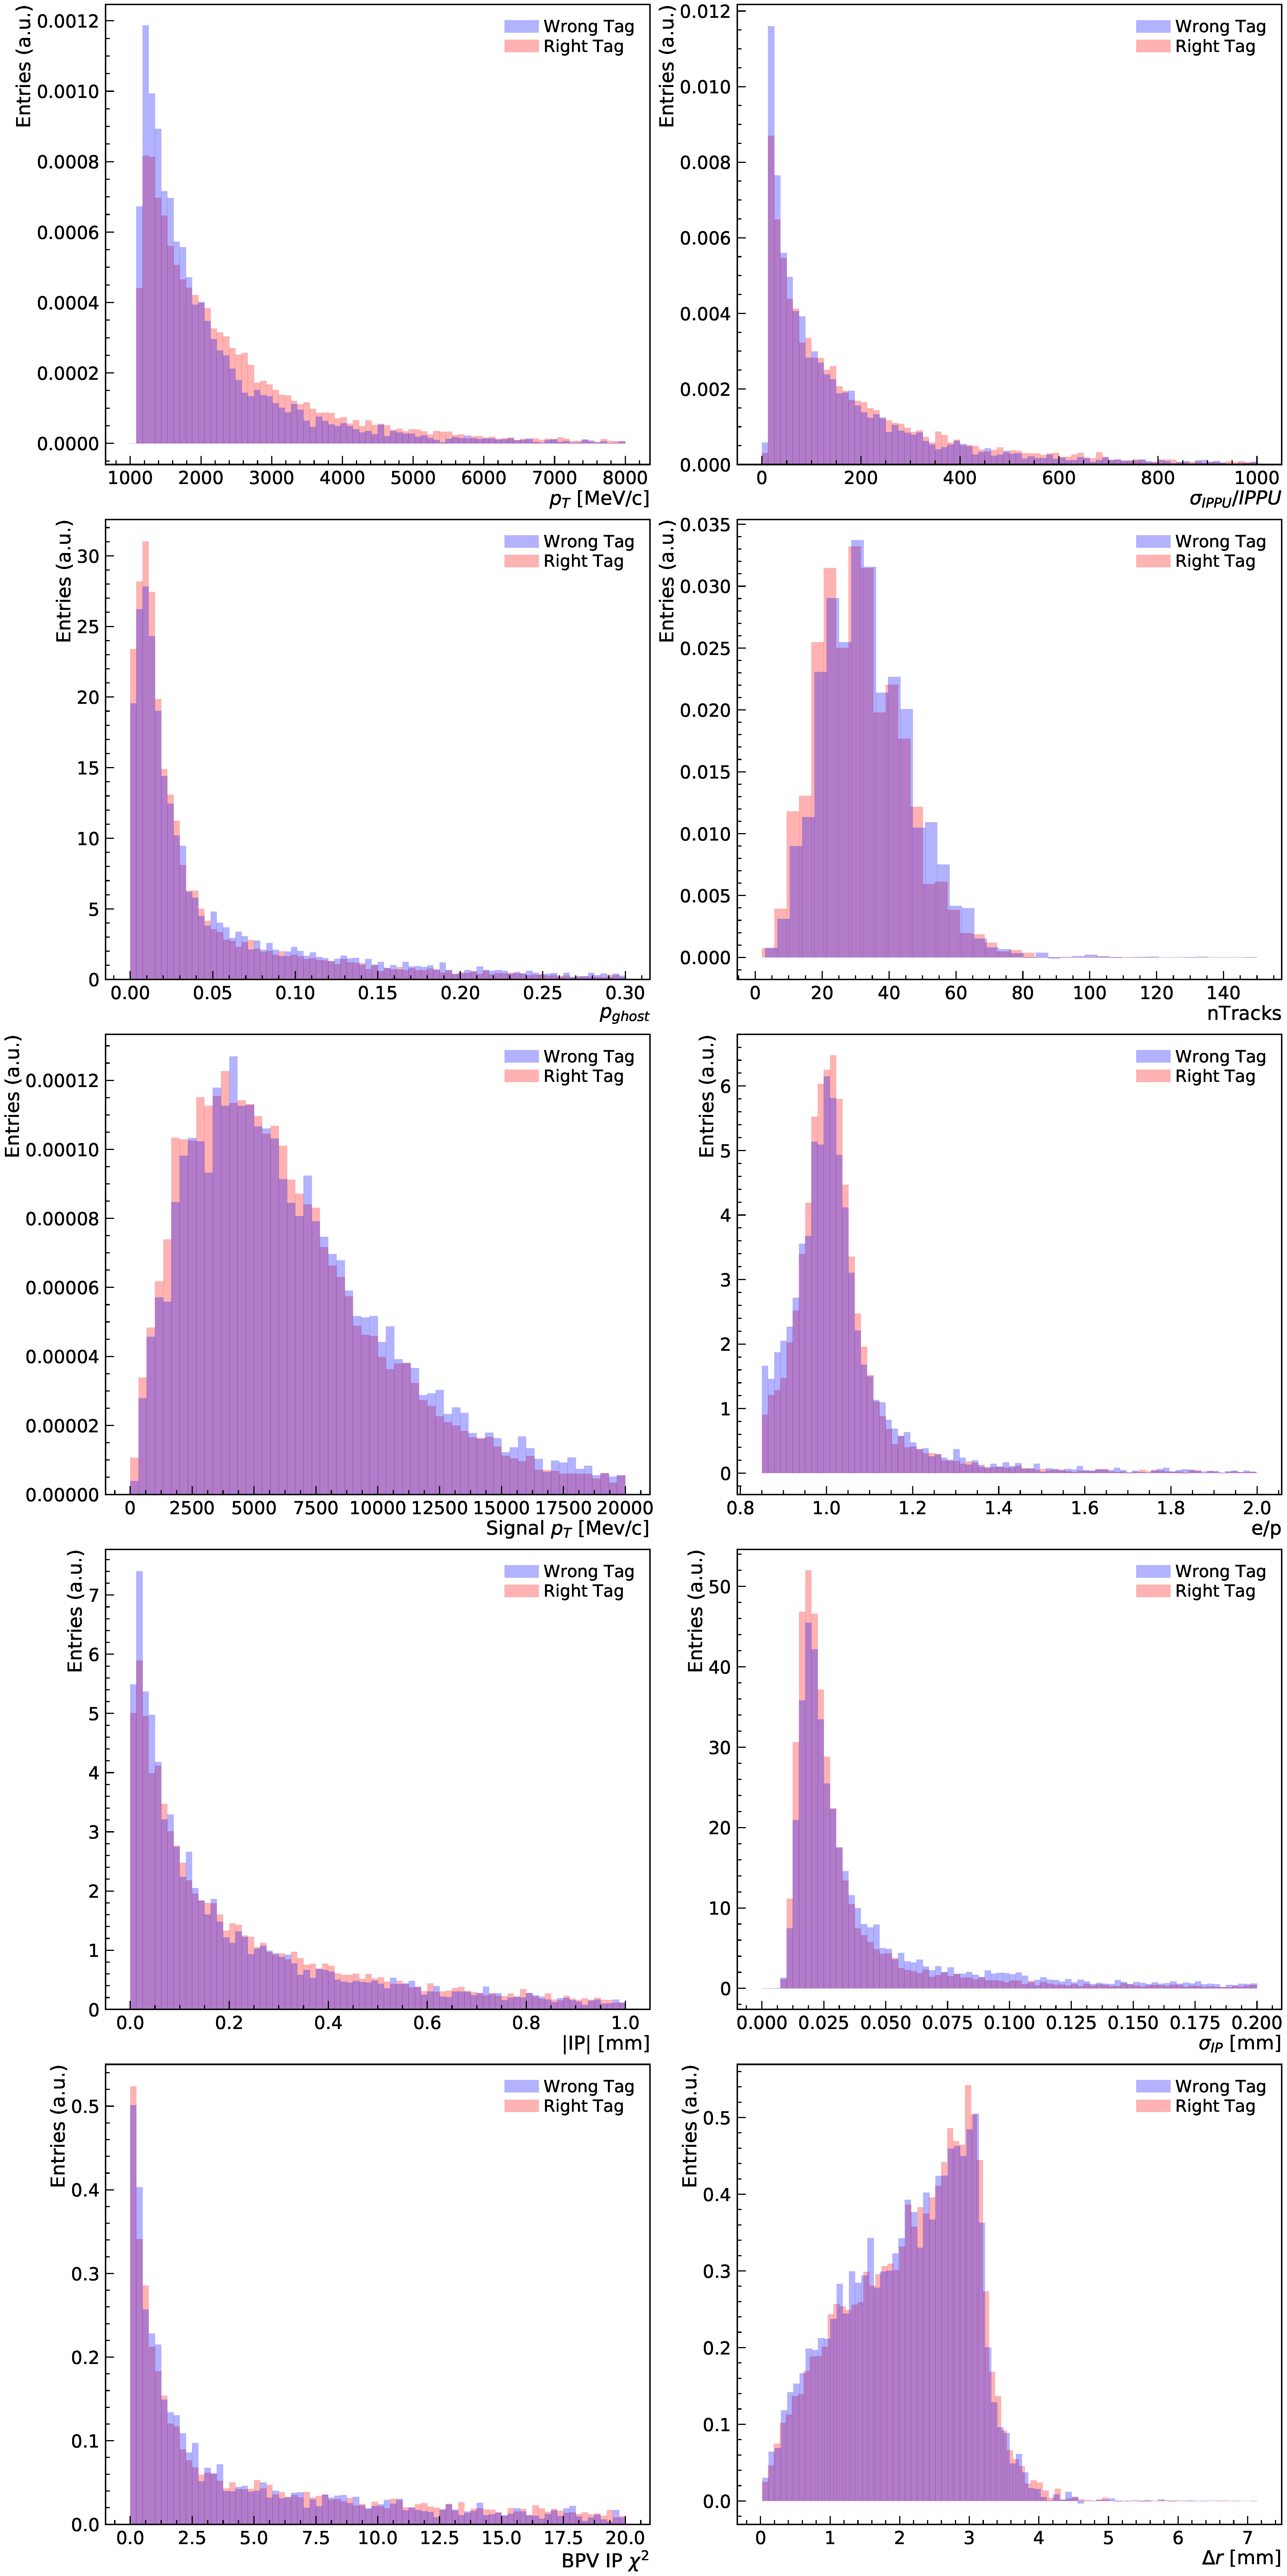
\includegraphics[width=0.7\textwidth]{04Flavourtagging/figs/OSelectronOpt/2017-12-12-vibattis-OSElectron-bdt-calibration-sWeights_Run1/FeaturesDistribution_RunIcuts.pdf}
        \end{center}
        \vspace{-2mm}
        \caption{Distributions (for the \emph{sWeighted}, Run 1 $B^+\to J/\psi K^+$ sample) of the input features of the BDT classifier, for candidates with a right (red) and wrong (blue) decision from the \OSe~tagger.}
         \label{fig:OSefeaturesRunI}
\end{figure}

\begin{figure}[htbp]
        \begin{center}
        \includegraphics[width=0.8\textwidth]{04Flavourtagging/figs/OSelectronOpt/2017-12-12-vibattis-OSElectron-bdt-calibration-sWeights_Run2/FeaturesDistribution_RunIIcuts.pdf}
        \end{center}
        \vspace{-2mm}
         \caption{Distributions (for the \emph{sWeighted}, Run 2 $B^+\to J/\psi K^+$ sample) of the input features of the BDT classifier, for candidates with a right (red) and wrong (blue) decision from the \OSe~tagger.}
         \label{fig:OSefeaturesRunIIB2CC}
\end{figure}

\begin{figure}[htbp]
        \begin{center}
        \includegraphics[width=0.8\textwidth]{04Flavourtagging/figs/OSelectronOpt/2018-04-07-vibattis-OSElectron-bdt-calibration-sWeights_Run2_Bu2D0pi/FeaturesDistribution_RunIIcuts.pdf}
        \end{center}
        \vspace{-2mm}
        \caption{Distributions (for the \emph{sWeighted}, Run 2 $B^+\to \Dzb \pi^+$ sample) of the input features of the BDT classifier, for candidates with a right (red) and wrong (blue) decision from the \OSe~tagger.}
         \label{fig:OSefeaturesRunIIB2OC}
\end{figure}

\begin{figure}[htbp]
        \begin{center}
        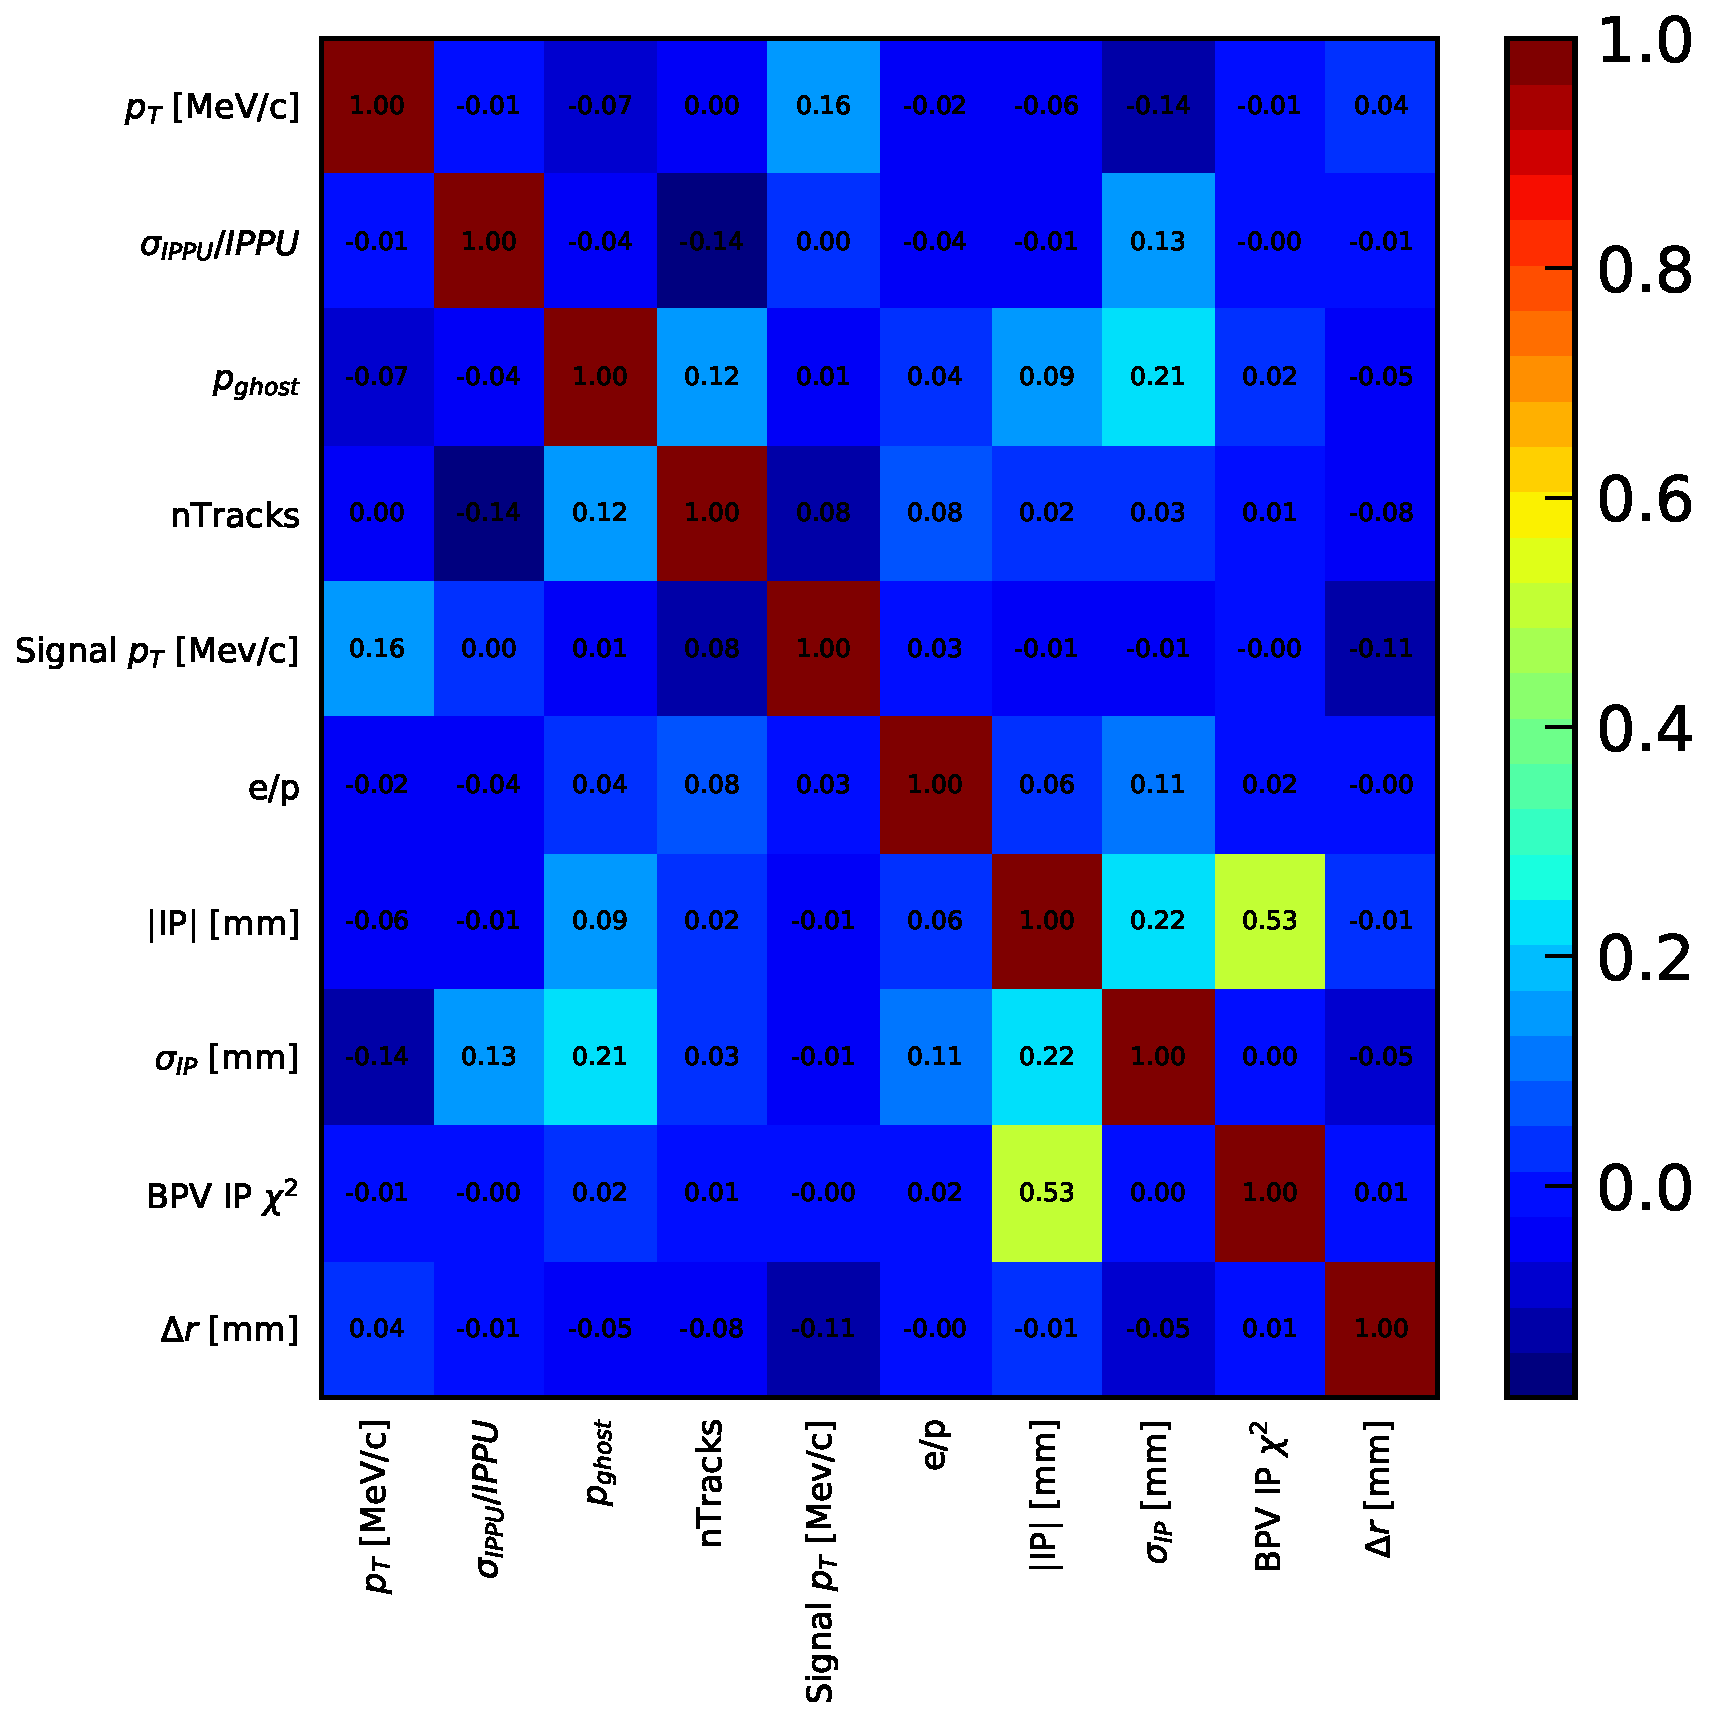
\includegraphics[width=0.47\textwidth]{04Flavourtagging/figs/OSelectronOpt/2017-12-12-vibattis-OSElectron-bdt-calibration-sWeights_Run1/FeaturesCorrRightTag_RunIcuts.pdf}
        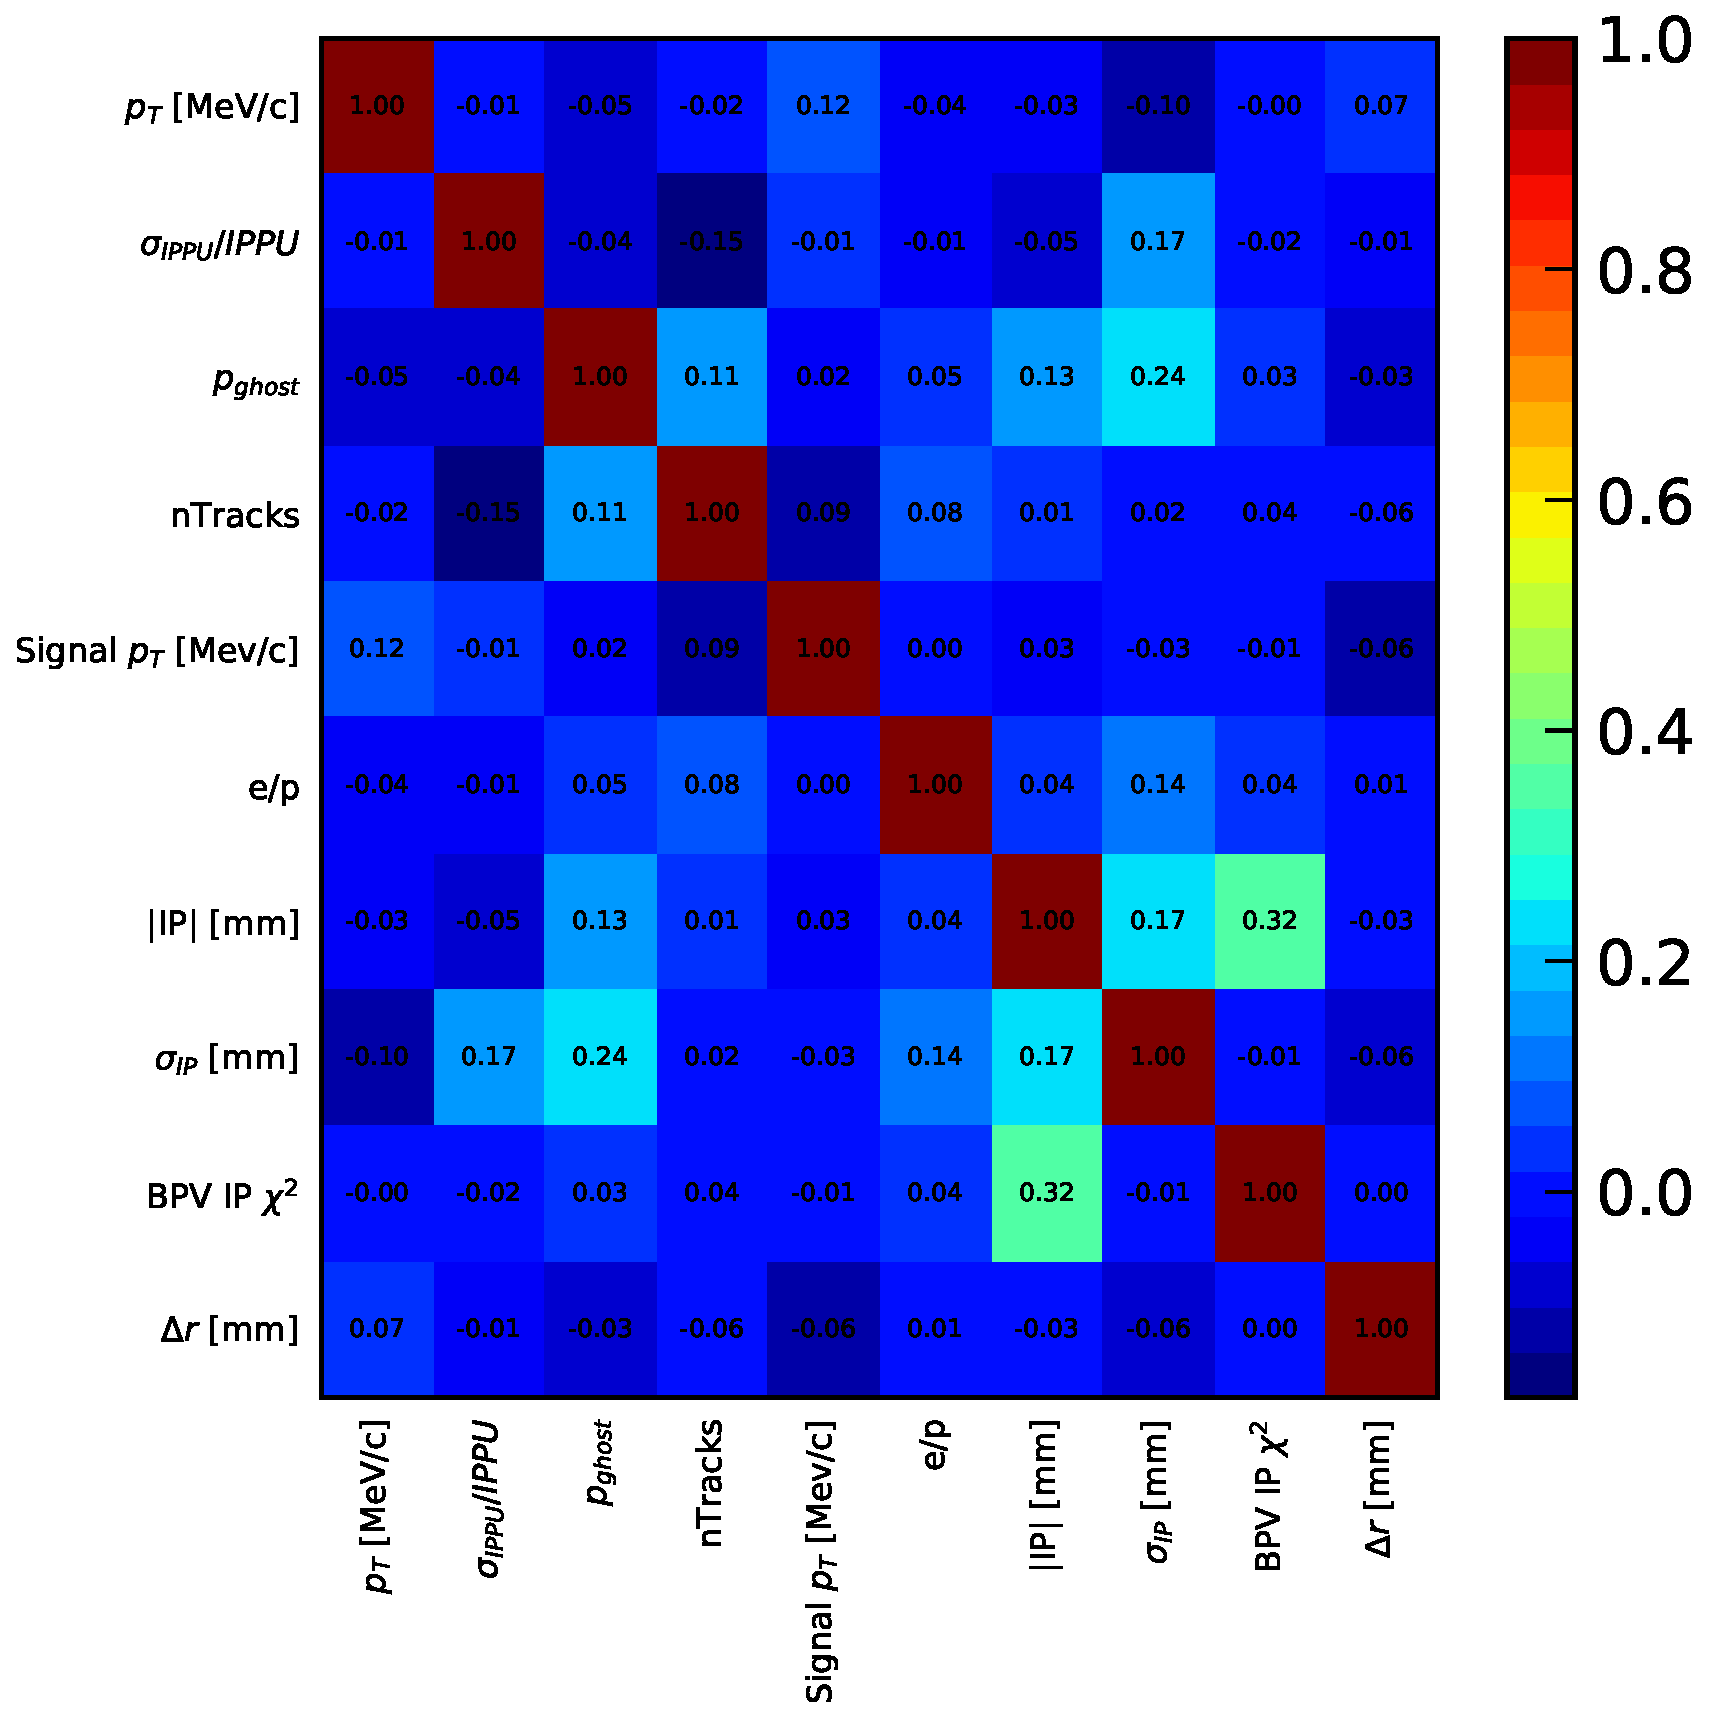
\includegraphics[width=0.47\textwidth]{04Flavourtagging/figs/OSelectronOpt/2017-12-12-vibattis-OSElectron-bdt-calibration-sWeights_Run1/FeaturesCorrWrongTag_RunIcuts.pdf} \\
        \includegraphics[width=0.47\textwidth]{04Flavourtagging/figs/OSelectronOpt/2017-12-12-vibattis-OSElectron-bdt-calibration-sWeights_Run2/FeaturesCorrRightTag_RunIIcuts.pdf}
        \includegraphics[width=0.47\textwidth]{04Flavourtagging/figs/OSelectronOpt/2017-12-12-vibattis-OSElectron-bdt-calibration-sWeights_Run2/FeaturesCorrWrongTag_RunIIcuts.pdf} \\
        \includegraphics[width=0.47\textwidth]{04Flavourtagging/figs/OSelectronOpt/2018-04-07-vibattis-OSElectron-bdt-calibration-sWeights_Run2_Bu2D0pi/FeaturesCorrRightTag_RunIIcuts.pdf}
        \includegraphics[width=0.47\textwidth]{04Flavourtagging/figs/OSelectronOpt/2018-04-07-vibattis-OSElectron-bdt-calibration-sWeights_Run2_Bu2D0pi/FeaturesCorrWrongTag_RunIIcuts.pdf} \\
        \end{center}
        \vspace{-2mm}
        \caption{Pearson correlation coefficients between the input features of the Run 1 new (top), Run 2 B2CC (middle) and Run 2 B2OC (bottom) BDT classifiers, for candidates with a correct (left) and wrong (right) decision from the \OSe~tagger.}
         \label{fig:OSecorrelations}
\end{figure}

The BDT classifier consists of an ensemble of 300 gradient-boosted decision trees~\cite{xgboost}, where each tree can have a maximum depth of 3. The objective of the classifier is a binary logistic loss function plus a quadratic regularisation term to control model complexity (with regularisation parameter $\lambda=1$). Some hyperparameters were tested by means of a cross-validation+bootstrapping method on the training set, as described in Appendix~\ref{app:oselectronappendix}. The importance (or F score) of each feature, defined as the total number of times a feature is chosen as split node by any tree in the BDT ensemble, is presented in Fig.~\ref{fig:OSeimportance}, while the \emph{partial dependence} of the predicted mistag $\eta$ (on the training set) as a function of each input feature is shown in Appendix~\ref{app:oselectronappendix}. 
The receiver operating characteristic (ROC) curves, which report the \emph{true positive rate}  
as a function of the \emph{false positive rate}, 
are shown in Fig.~\ref{fig:OSerocs}. 
The true (false) positive rate is the fraction of true, correctly (incorrectly) tagged candidates over all candidates classified as correctly tagged. 
The feature selection, BDT training and feature importance evaluation chain is repeated iteratively in order to exclude highly-correlated and poorly-important features, until the BDT performance starts to degrade significantly.

\begin{figure}[t]
        \begin{center}
        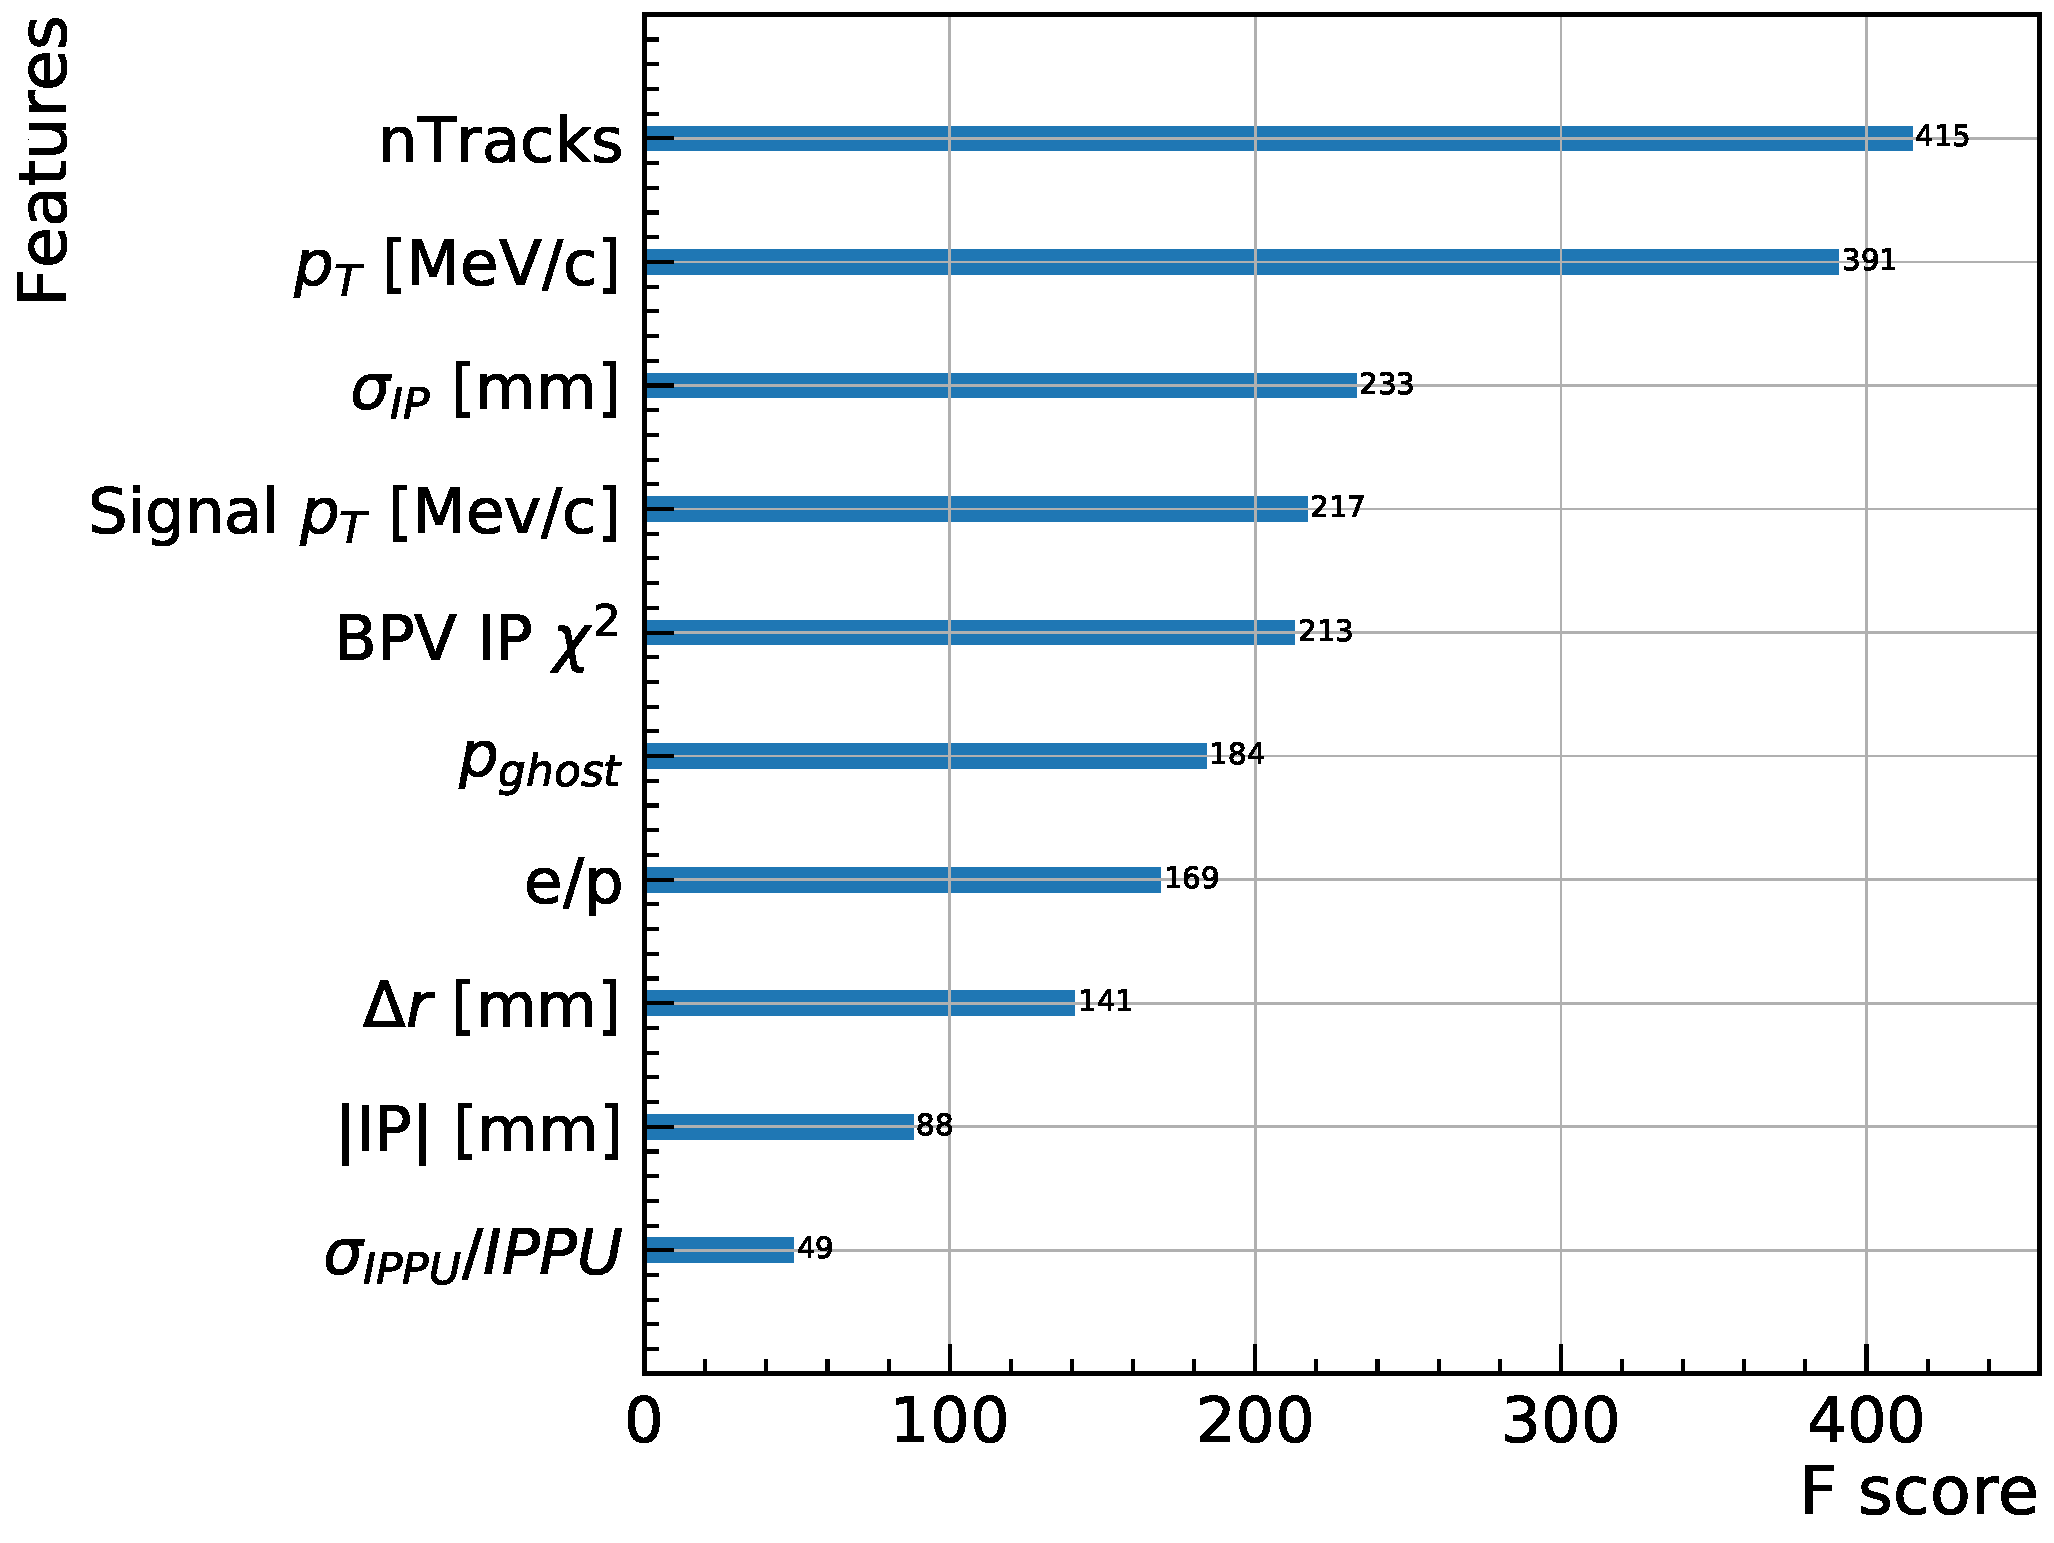
\includegraphics[width=0.4\textwidth]{04Flavourtagging/figs/OSelectronOpt/2017-12-12-vibattis-OSElectron-bdt-calibration-sWeights_Run1/Importance_RunIcuts.pdf}
        \includegraphics[width=0.4\textwidth]{04Flavourtagging/figs/OSelectronOpt/2017-12-12-vibattis-OSElectron-bdt-calibration-sWeights_Run2/Importance_RunIIcuts.pdf} \\
        \includegraphics[width=0.4\textwidth]{04Flavourtagging/figs/OSelectronOpt/2018-04-07-vibattis-OSElectron-bdt-calibration-sWeights_Run2_Bu2D0pi/Importance_RunIIcuts.pdf}
        \end{center}
        \vspace{-2mm}
        \caption{Feature importance for the BDT classifiers of the Run 1 new (top left), Run 2 B2CC (top right) and Run 2 B2OC (bottom) implementations of the \OSe~tagger.}
         \label{fig:OSeimportance}
\end{figure}

\begin{figure}[t]
        \begin{center}
        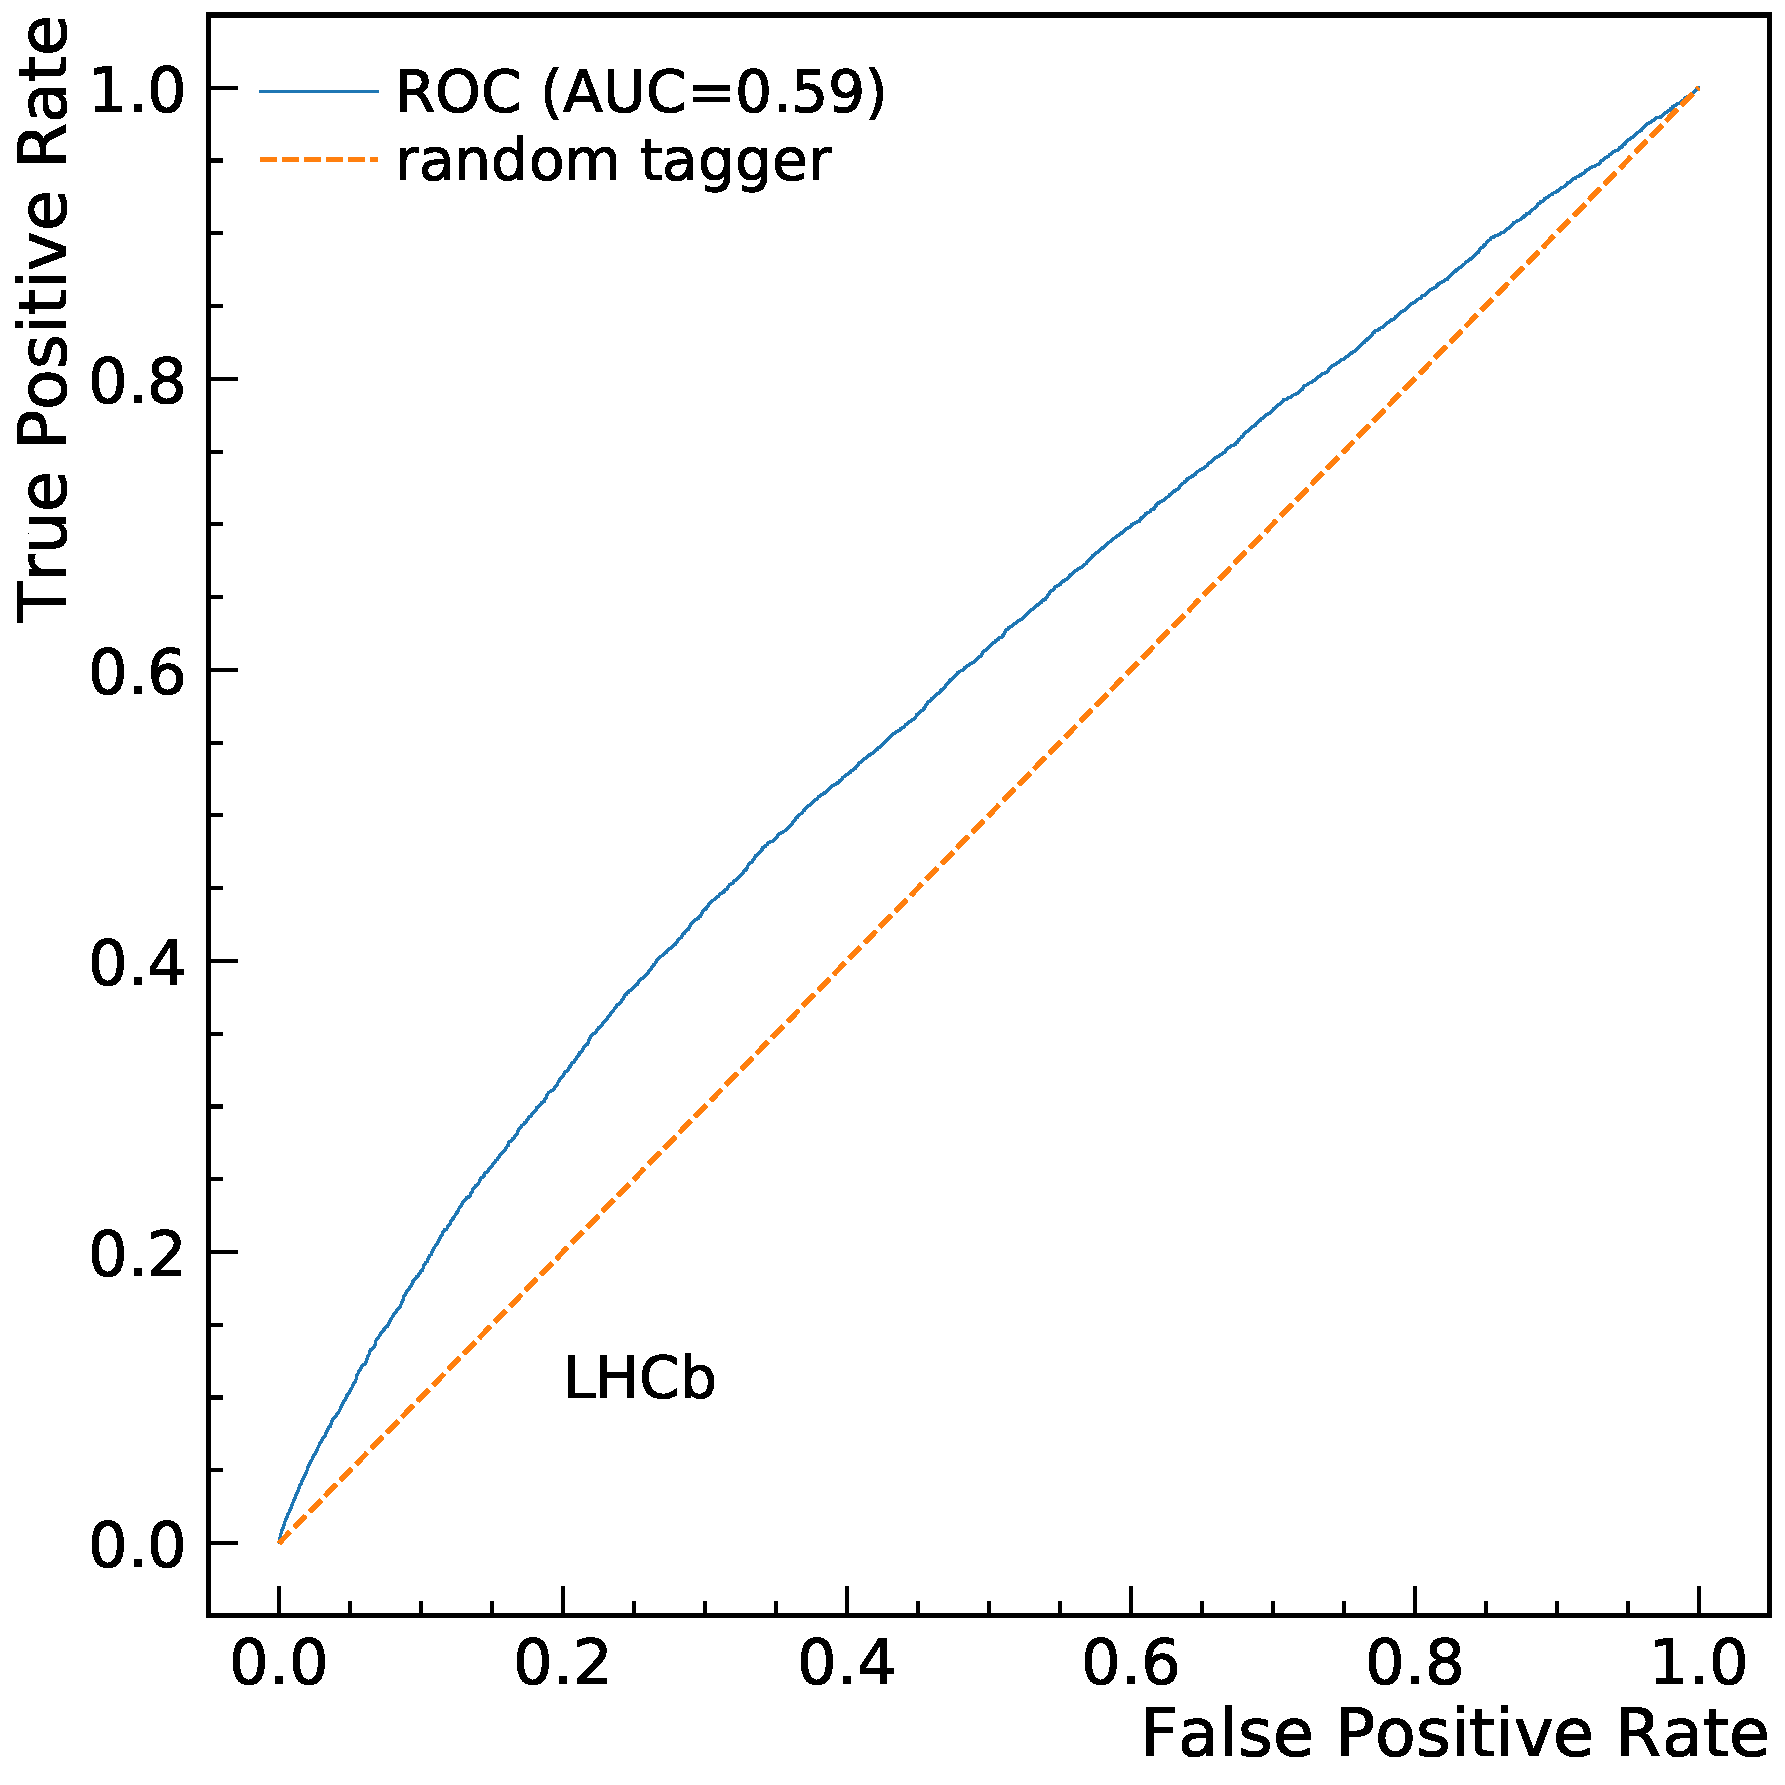
\includegraphics[width=0.4\textwidth]{04Flavourtagging/figs/OSelectronOpt/2017-12-12-vibattis-OSElectron-bdt-calibration-sWeights_Run1/ROC_RunIcuts.pdf}
        \includegraphics[width=0.4\textwidth]{04Flavourtagging/figs/OSelectronOpt/2017-12-12-vibattis-OSElectron-bdt-calibration-sWeights_Run2/ROC_RunIIcuts.pdf} \\
        \includegraphics[width=0.4\textwidth]{04Flavourtagging/figs/OSelectronOpt/2018-04-07-vibattis-OSElectron-bdt-calibration-sWeights_Run2_Bu2D0pi/ROC_RunIIcuts.pdf}
        \end{center}
        \vspace{-2mm}
        \caption{True positive rate as a function of the false positive rate (ROC curves) for the BDT classifiers of the Run 1 new (top left), Run 2 B2CC (top right) and Run 2 B2OC (bottom) implementations of \OSe. The obtained ROC curves are represented in blue, while the expected ROC curve in case of random tag decision is shown as a dashed orange line. For each BDT, the \emph{Area Under the} ROC \emph{Curve} (AUC score) is reported as well.}
         \label{fig:OSerocs}
\end{figure}

For each candidate, the BDT predicts the probability $P$ that such candidates is correctly tagged. In order to obtain a mistag probability $\eta$, the following transformation is applied on both $P$ and tagging decision $d$:
\begin{equation}
        (\eta, d) \rightarrow \begin{cases} (P, -d) &\text{if $P\leq0.5$} \\ (1-P, d) &\text{otherwise} \end{cases}        
\end{equation} 
The distributions of $\eta$ for training and test samples, splitted per target value, are shown in Fig.~\ref{fig:OSeetapredict}.

\begin{figure}[t]
        \begin{center}
        \includegraphics[width=0.4\textwidth]{04Flavourtagging/figs/OSelectronOpt/2017-12-12-vibattis-OSElectron-bdt-calibration-sWeights_Run1/PredictedEta_RunIcuts.pdf}
        \includegraphics[width=0.4\textwidth]{04Flavourtagging/figs/OSelectronOpt/2017-12-12-vibattis-OSElectron-bdt-calibration-sWeights_Run2/PredictedEta_RunIIcuts.pdf}
        \includegraphics[width=0.4\textwidth]{04Flavourtagging/figs/OSelectronOpt/2018-04-07-vibattis-OSElectron-bdt-calibration-sWeights_Run2_Bu2D0pi/PredictedEta_RunIIcuts.pdf}
        \end{center}
        \vspace{-2mm}
        \caption{\emph{sWeighted} distributions of the mistag probability $\eta$ predicted by the BDT classifiers of the Run 1 new (top left), Run 2 B2CC (top right) and Run 2 B2OC (bottom) versions of the \OSe~tagger. 
          The blue-solid (red-hatched) histogram represents the training data for candidates having the wrong (right) tag decision. 
          The blue (red) points indicate the test data for candidates with wrong (right) tag decision. 
          The overtraining is checked, separately for candidates with wrong and right tag decision,
          by means of a Kologorov-Smirnov (KS) test to measure the compatibility between training data and test data.
          The conventional value of $0.05$ is chosen as significance level to reject the hypothesis of compatibility.}
        \label{fig:OSeetapredict}
\end{figure}

%%%%%%%%%%%%%%%%%%%%%%%%%%%%%%%%%%%%%%%%%%%%%%%%%%%%

\subsection{Performance evaluation}

%%%%%%%%%%%%%%%%%%%%%%%%%%%%%%%%%%%%%%%%%%%%%%%%%%%%

\subsubsection[Performance on $B^+\to J/\psi K^+$ and $B^+\to \Dzb \pi^+$ data]{Performance on \boldmath{$B^+\to J/\psi K^+$} and \boldmath{$B^+\to \Dzb \pi^+$} data}
\label{sec:tagging:OSePerf1}

Once the BDT is trained on the training ssample, the mistag $\eta$ is predicted for each candidate using the evaluation samples. Then, a two-fold evaluation is applied:
\begin{itemize}[noitemsep,topsep=0pt]
        \item the mistag calibration is determined on the first evaluation sample. The obtained calibration is then applied to the second evaluation sample, and a calibrated per-event tagging power is computed on the latter;
        \item same as above, but with the two evaluation samples swapped.
\end{itemize}
The calibrated per-event tagging power is computed by considering, for each tagged $B$ candidate, only the tagging particle with the highest transverse momentum.
The calibration model consists of a first order natural spline with a logistic link function.
The result of these calibrations are shown in Fig.~\ref{fig:OSeetacalib}.
The calibrated per-event tagging power is reported in Table~\ref{tab:OSeperformanceevalset}.

\begin{figure}[t]
        \begin{center}
        \includegraphics[width=0.4\textwidth]{04Flavourtagging/figs/OSelectronOpt/RunIEval_Bu2JpsiKst/eval_on_I.pdf}
        \includegraphics[width=0.4\textwidth]{04Flavourtagging/figs/OSelectronOpt/RunIEval_Bu2JpsiKst/eval_on_II.pdf} \\
        \includegraphics[width=0.4\textwidth]{04Flavourtagging/figs/OSelectronOpt/RunIIEval_Bu2JpsiKst/eval_on_I.pdf}
        \includegraphics[width=0.4\textwidth]{04Flavourtagging/figs/OSelectronOpt/RunIIEval_Bu2JpsiKst/eval_on_II.pdf} \\
        \includegraphics[width=0.4\textwidth]{04Flavourtagging/figs/OSelectronOpt/RunIIEval_Bu2D0Pi/eval_on_I.pdf}
        \includegraphics[width=0.4\textwidth]{04Flavourtagging/figs/OSelectronOpt/RunIIEval_Bu2D0Pi/eval_on_II.pdf}
        \end{center}
        \vspace{-2mm}
        \caption{\OSe~mistag calibration results for the (top) Run 1 new, (middle) Run 2 B2CC and (bottom) Run 2 B2OC optimisations. Left: calibration obtained on the second evaluation sample plotted together with the first evaluation sample. Right: calibration obtained on the first evaluation sample plotted together with the second evaluation sample. The \emph{sWeighted} data sample is shown as black points. The green (yellow) band indicates the 68\% (95\%) C.L. interval for the fitted calibration functions.}
        \label{fig:OSeetacalib}
\end{figure}

\begin{table}[t]
	\centering
        \caption{Calibrated, per-event tagging power $\effeff$ (in $\%$) of the \OSe~algorithms obtained on the evaluation sets of each \OSe~implementation. The errors include both statistical uncertainty and uncertainties from the calibration procedure. The average is computed by assuming uncorrelated measurements.}
         \label{tab:OSeperformanceevalset}
        \begin{tabular}{llll}
        \toprule
        Algorithm & set 1 & set 2 & average  \\
        \midrule
        Run 1 new & $0.513\pm0.040$ & $0.496\pm0.038$ & $0.504\pm0.028$ \\
        Run 2 B2CC & $0.324\pm0.031$ & $0.364\pm0.033$ & $0.343\pm0.023$ \\
        Run 2 B2OC & $0.455\pm0.043$ & $0.434\pm0.041$ & $0.444\pm0.030$ \\
        \bottomrule
        \end{tabular}
\end{table}

%%%%%%%%%%%%%%%%%%%%%%%%%%%%%%%%%%%%%%%%%%%%%%%%%%%%

\subsubsection[Performance on $B^0\to D^-\pi^+$ data]{Performance on \boldmath{$B^0\to D^-\pi^+$} data}
\label{sec:tagging:OSePerf2}

The performance (tagging efficiency, mistag probability, tagging power) of the calibrated \OSe~tagger is evaluated on Run 1 (2012) and Run 2 (2016) \emph{sWeighted} data samples of $B^0\to D^-\pi^+$ decays.
These decays ensure a robust estimation of the performance thanks to the high statistics collected at LHCb. Moreover, this channel was not exploited in the development of
the \OSe~tagger, so that it constitutes an independent validation of these algorithms. The performance of the other OS taggers (\OSmu, \OSK, \OSc, \OSvtx, and their combination) is presented
as well in this section in order to provide a complete overview.

The calibration and the performance evaluation are done as follows:
\begin{itemize}[noitemsep,topsep=0pt]
  \item each sample (Run 1 and Run 2) is split randomly in two subsamples;
    \item the calibrations are found on one subsample for all OS taggers;
      \item the obtained calibrations are applied to the other subsample, and the calibrated performance is evaluated.
        \item the calibrated OS taggers are combined, the combination is calibrated in order to correct for effects due to correlations among taggers, and the performance of the calibrated combination is evaluated.
\end{itemize}

The calibrations are obtained via a time-dependent analysis of the $B^0\to D^-\pi^+$ decays, where acceptance and resolution effects are neglected as described in Ref.~\cite{EPM}; moreover, the Cabibbo-suppressed decay mode $B^0\to D^+\pi^-$ is ignored as well.
The chosen model 
$\omega(\eta)$ for each tagger is a GLM model with a logistic link function, and a first order spline as basis function. The results of the calibration and the mistag distribution of each \OSe~implementation are shown in Figs.~\ref{fig:OSePerfCalib1} and~\ref{fig:OSePerfCalib3}; the calibration and the mistag of the corresponding OS combinations are also reported in Figs.~\ref{fig:OSePerfCalib2} and~\ref{fig:OSePerfCalib4}.
 
\begin{figure}[ht!]
        \centering
        \includegraphics[width=0.26\textwidth]{04FlavourTagging/figs/OSelectronOpt/run1data_old/OS_Electron_InputCalibration.pdf}
        \includegraphics[width=0.26\textwidth]{04FlavourTagging/figs/OSelectronOpt/run1data_new/OS_Electron_InputCalibration.pdf} \\
        \includegraphics[width=0.26\textwidth]{04FlavourTagging/figs/OSelectronOpt/run1data_old/OS_Electron_EtaDist.pdf}
        \includegraphics[width=0.26\textwidth]{04FlavourTagging/figs/OSelectronOpt/run1data_new/OS_Electron_EtaDist.pdf}
        \vspace{-2mm}
        \caption{Top: mistag calibration results on \emph{sWeighted} Run 1 $B^0\to D^-\pi^+$ data for the Run 1 old (left) and Run 1 new (right) versions of the \OSe~tagger. The \emph{sWeighted} data sample is shown as black points. The green (yellow) band indicates the 68\% (95\%) C.L. interval for the fitted calibration functions. Bottom: distributions of the uncalibrated mistag $\eta$.}
        \label{fig:OSePerfCalib1}
\end{figure}

\begin{figure}[hb!]
  \centering
  \includegraphics[width=0.26\textwidth]{04FlavourTagging/figs/OSelectronOpt/run1_tunings/OS_Electron_InputCalibration.pdf}
  \includegraphics[width=0.26\textwidth]{04FlavourTagging/figs/OSelectronOpt/run2b2cc_tunings/OS_Electron_InputCalibration.pdf}
  \includegraphics[width=0.26\textwidth]{04FlavourTagging/figs/OSelectronOpt/run2b2oc_tunings/OS_Electron_InputCalibration.pdf} \\
  \includegraphics[width=0.26\textwidth]{04FlavourTagging/figs/OSelectronOpt/run1_tunings/OS_Electron_EtaDist.pdf}
  \includegraphics[width=0.26\textwidth]{04FlavourTagging/figs/OSelectronOpt/run2b2cc_tunings/OS_Electron_EtaDist.pdf}
  \includegraphics[width=0.26\textwidth]{04FlavourTagging/figs/OSelectronOpt/run2b2oc_tunings/OS_Electron_EtaDist.pdf}
  \caption{Mistag calibration results on \emph{sWeighted} Run 2 $B^0\to D^-\pi^+$ data for the \OSe~taggers. The results obtained with the Run 1 old (left), Run 2 B2CC (center), and Run 2 B2OC (right) tunings are shown.
The \emph{sWeighted} data sample is shown as black points. The green (yellow) band indicates the 68\% (95\%) C.L. interval for the fitted calibration functions. Bottom: distributions of the uncalibrated mistag $\eta$.}
  \label{fig:OSePerfCalib3}
\end{figure}


\begin{figure}[ht!]
  \centering
  \includegraphics[width=0.26\textwidth]{04FlavourTagging/figs/OSelectronOpt/run1data_old/OS_Combination_Calibration.pdf}
  \includegraphics[width=0.26\textwidth]{04FlavourTagging/figs/OSelectronOpt/run1data_new/OS_Combination_Calibration.pdf} \\
  \includegraphics[width=0.26\textwidth]{04FlavourTagging/figs/OSelectronOpt/run1data_old/OS_Combination_EtaDist.pdf}
  \includegraphics[width=0.26\textwidth]{04FlavourTagging/figs/OSelectronOpt/run1data_new/OS_Combination_EtaDist.pdf} 
  \vspace{-2mm}
  \caption{Top: mistag calibration results on \emph{sWeighted} Run 1 $B^0\to D^-\pi^+$ data for the combination of the OS taggers. The results obtained with the Run 1 old (left) and Run 1 new (right) tunings of \OSe~are shown. The \emph{sWeighted} data sample is shown as black points. The green (yellow) band indicates the 68\% (95\%) C.L. interval for the fitted calibration functions. Bottom: distributions of the uncalibrated mistag $\eta$.}
  \label{fig:OSePerfCalib2}
\end{figure}

\begin{figure}[hb!]
  \centering
  \includegraphics[width=0.26\textwidth]{04FlavourTagging/figs/OSelectronOpt/run1_tunings/OS_Combination_Calibration.pdf}
  \includegraphics[width=0.26\textwidth]{04FlavourTagging/figs/OSelectronOpt/run2b2cc_tunings/OS_Combination_Calibration.pdf}
  \includegraphics[width=0.26\textwidth]{04FlavourTagging/figs/OSelectronOpt/run2b2oc_tunings/OS_Combination_Calibration.pdf} \\
  \includegraphics[width=0.26\textwidth]{04FlavourTagging/figs/OSelectronOpt/run1_tunings/OS_Combination_EtaDist.pdf}
  \includegraphics[width=0.26\textwidth]{04FlavourTagging/figs/OSelectronOpt/run2b2cc_tunings/OS_Combination_EtaDist.pdf}
  \includegraphics[width=0.26\textwidth]{04FlavourTagging/figs/OSelectronOpt/run2b2oc_tunings/OS_Combination_EtaDist.pdf}
  \vspace{-2mm}
  \caption{Mistag calibration results on \emph{sWeighted} Run 2 $B^0\to D^-\pi^+$ data for the combination of the OS taggers. The results obtained with the Run 1 old (left), Run 2 B2CC (center), and Run 2 B2OC (right) tunings of \OSe, \OSmu, and \OSK~are shown. The \emph{sWeighted} data sample is shown as black points. The green (yellow) band indicates the 68\% (95\%) C.L. interval for the fitted calibration functions. Bottom: distributions of the uncalibrated mistag $\eta$.}
  \label{fig:OSePerfCalib4}
\end{figure}

The performance is reported in Tables~\ref{tab:Bd2DpiperformanceRun1}~and~\ref{tab:Bd2DpiperformanceRun2}.
The Run 1 new tuning allows to gain a relative $~9\%$ in tagging power for the \OSe~tagger on Run 1 data; the corresponding, relative gain of the OS combination is $~3\%$.
The tagging power of \OSvtx~and \OSc, which were trained on Run 1 data, increases on Run 2 data compared to Run 1; 
for this reason, no specific optimisation for the Run 2 conditions is performed.
The tagging power of \OSe, \OSmu, and \OSK~with the Run 1 tunings is lower on Run 2 data compared to Run 1. 
However, compared to the Run 1 tunings, the Run 2 tunings show a relative improvement in tagging power of about $\sim 160\%$ for \OSe, and $\sim 6\%$ for \OSmu~and \OSK~on Run 2 data. This allows to recover similar performances as the ones obtained on Run 1 data with the Run 1 tunings, both for the individual taggers and their combination.
Moreover, the Run 2 B2CC and B2OC tunings show consistent tagging powers on Run 2 data, meaning that the optimisation is robust against the different kinematics of the adopted decays.

\begin{table}
\centering
\caption{Performance (tagging efficiency, average mistag and tagging power in $\%$) of the OS taggers on \emph{sWeighted} Run 1 $B^0\to D^-\pi^+$ data. The numbers for \OSe~and the OS combination are shown separately for the Run 1 old and Run 1 new tunings. The first uncertainty is statistical and the second comes from the calibration.}
\label{tab:Bd2DpiperformanceRun1}
%\resizebox{\textwidth}{!}{
\begin{tabular*}{\textwidth}{rlllll}
\toprule
\multicolumn{1}{c}{Tagger} & \multicolumn{1}{c}{$\etag$} & \multicolumn{1}{c}{$\avg{\mistag}$} & \multicolumn{1}{c}{$\effeff$} \\
\midrule
\OSvtx& $22.026\pm0.100$& $37.295\pm0.030\pm0.376$& $1.422\pm0.009\pm0.084$\\
\OSc& $4.632\pm0.050$& $34.026\pm0.049\pm0.824$& $0.473\pm0.006\pm0.049$\\
\hline
\OSe~Run 1 old& $3.028\pm0.041$& $30.570\pm0.113\pm0.963$& $0.457\pm0.008\pm0.045$\\
\OSe~Run 1 new& $4.337\pm0.049$& $33.089\pm0.085\pm0.777$& $0.496\pm0.007\pm0.046$\\
\hline
\OSmu~Run 1& $8.539\pm0.067$& $28.756\pm0.071\pm0.582$& $1.541\pm0.016\pm0.085$\\
\hline
\OSK~Run 1& $18.800\pm0.094$& $36.724\pm0.031\pm0.417$& $1.325\pm0.009\pm0.083$\\
\hline
\begin{tabular}{c} OS combination \\ Run 1 old \end{tabular}& $39.004\pm0.117$& $34.679\pm0.035\pm0.273$& $3.662\pm0.020\pm0.131$\\
\begin{tabular}{c} OS combination \\ Run 1 new \end{tabular}& $39.733\pm0.118$& $34.576\pm0.035\pm0.270$& $3.781\pm0.021\pm0.133$\\
\bottomrule
\end{tabular*}
%}
\end{table}

\begin{table}
\centering
\caption{Performance (tagging efficiency, average mistag and tagging power in $\%$) of the OS taggers on \emph{sWeighted} Run 2 $B^0\to D^-\pi^+$ data. The numbers for \OSe, \OSmu, \OSK, and the OS combination are shown separately for the Run 1, Run 2 B2CC, and Run 2 B2OC tunings. The first uncertainty is statistical and the second comes from the calibration.}
\label{tab:Bd2DpiperformanceRun2}
%\resizebox{\textwidth}{!}{
\begin{tabular*}{\textwidth}{rlllll}
\toprule
\multicolumn{1}{c}{Tagger} & \multicolumn{1}{c}{$\etag$} & \multicolumn{1}{c}{$\avg{\mistag}$} & \multicolumn{1}{c}{$\effeff$} \\
\midrule
\OSvtx& $20.834\pm0.075$& $36.139\pm0.029\pm0.301$& $1.601\pm0.009\pm0.070$\\ 
\OSc& $5.025\pm0.040$& $33.875\pm0.041\pm0.624$& $0.523\pm0.005\pm0.040$\\
\hline
\OSe~Run 1 old& $1.868\pm0.025$& $34.300\pm0.096\pm0.941$& $0.184\pm0.003\pm0.022$\\
\OSe~Run 2 B2CC& $4.451\pm0.038$& $33.352\pm0.081\pm0.608$& $0.493\pm0.006\pm0.036$\\
\OSe~Run 2 B2OC& $3.333\pm0.033$& $30.917\pm0.075\pm0.702$& $0.486\pm0.006\pm0.036$\\
\hline
\OSmu~Run 1& $8.343\pm0.051$& $30.357\pm0.042\pm0.466$& $1.288\pm0.010\pm0.061$\\
\OSmu~Run 2 B2CC& $9.151\pm0.053$& $30.837\pm0.041\pm0.432$& $1.344\pm0.010\pm0.061$\\
\OSmu~Run 2 B2OC& $8.040\pm0.050$& $29.174\pm0.043\pm0.463$& $1.395\pm0.010\pm0.062$\\
\hline
\OSK~Run 1& $15.737\pm0.067$& $35.902\pm0.030\pm0.357$& $1.251\pm0.008\pm0.063$\\
\OSK~Run 2 B2CC& $19.516\pm0.073$& $36.889\pm0.026\pm0.310$& $1.342\pm0.007\pm0.064$\\
\OSK~Run 2 B2OC& $15.793\pm0.067$& $35.565\pm0.030\pm0.348$& $1.316\pm0.008\pm0.063$\\
\hline
\begin{tabular}{c} OS combination \\ Run 1 old \end{tabular}& $36.239\pm0.088$& $35.285\pm0.024\pm0.227$& $3.139\pm0.013\pm0.097$\\
\begin{tabular}{c} OS combination \\ Run 2 B2CC \end{tabular}& $40.154\pm0.090$& $35.123\pm0.025\pm0.210$& $3.555\pm0.014\pm0.100$\\
\begin{tabular}{c} OS combination \\ Run 2 B2OC \end{tabular}& $36.555\pm0.089$& $34.225\pm0.026\pm0.220$& $3.638\pm0.015\pm0.102$\\
\bottomrule
\end{tabular*}
%}
\end{table}



\chapter{Selection of \boldmath{$B^0\to D^{\mp}\pi^{\pm}$} decays}
\clearpage
%!TEX root = ../my_thesis.tex
\section{Data sample and preselection}
\label{sec:sample_and_selection}

%===============================================================================
The sample of data is passed through the following selection steps:
\begin{enumerate}[noitemsep,topsep=0pt]
	\item stripping and trigger requirements;
	\item a \emph{cut-based} preselection;
	\item vetoes for misidentified backgrounds and wrongly associated \emph{primary vertices} (PVs);
	\item a multivariate classification (MVA);
	\item a final randomised multiple candidate selection.
\end{enumerate}
In what follows, the details of each step are provided.

%===============================================================================
\subsection{Stripping and trigger requirements}
\label{sec:stripping}

Signal $\Bz\to\Dmp\pipm$ candidates are reconstructed using a dedicated stripping line
(called \verb!B02DPiD2HHHBeauty2CharmLine!). Each event is required to have less than
\num{500} long tracks. The criteria that the charged tracks have to
fulfill are listed in Table~\ref{tab:strippingDaughters}.
%
\begin{table}[b!]
	\centering
	\caption{Stripping requirements applied in the selection of charged tracks. The more stringent
	  requirements given in brackets are for the bachelor track. The IP$\chi^2$ is 
          the vertex-fit $\chi^2$ difference for the PV reconstructed with and without the $\Bz$ candidate.}
	\begin{tabular}{cc}
		\toprule
		track $\chi^2/$ndof & $<\num{3.0}$ ($<\num{2.5}$)\\
		momentum $p$ & $>\SI{1}{\GeVc}$ ($>\SI{5}{\GeVc}$)\\
		transverse momentum $\pt$ & $>\SI{100}{\MeVc}$ ($>\SI{500}{\MeVc}$)\\
		IP$\chi^2$ w.r.t. any PV & $>\num{4.0}$\\
		ghost probability & $<\num{0.4}$\\
		\bottomrule
	\end{tabular}
	\label{tab:strippingDaughters}
\end{table}
%
Three of these hadrons have to form a common vertex to build a $\Dmp$ meson. 
Further requirements on the \Dmp~combination are given in
Table~\ref{tab:strippingD}.
%
\begin{table}[htbp]
	\centering
	\caption{Stripping requirements on the three-track combinations forming $\Dmp$ candidates. DOCA is the Distance Of
	  Closest Approach of the daughter particles w.r.t. each other, and
	  DIRA indicates the cosine of the angle between the momentum of the $\Dmp$
	  meson and the direction from the best PV to the decay vertex. The best PV is defined as
	  the vertex with the lowest IP$\chi^2$.}
	\begin{tabular}{cc}
		\toprule
		$\sum$ $\pt(hhh)$ & $>\SI{1800}{\MeVc}$\\
		DOCA & $<\SI{0.5}{\milli\metre}$\\
		$m(hhh)$ & $\in[1769.62,2068.49]\mevcc$\\
		$\Dmp$ vertex $\chi^2/$ndof & $<\num{10.0}$\\
		$\Dmp$ vertex separation $\chisq$ to any PV & $>\num{36}$\\
		$\Dmp$ DIRA & $>\num{0.0}$\\
		\bottomrule
	\end{tabular}
	\label{tab:strippingD}
\end{table}
%
The $\Bz$ candidates are built by combining a $\Dmp$ candidate and a bachelor
particle if the requirements listed in Table~\ref{tab:strippingB} are fulfilled.
Finally, a bagged boosted decision tree (BDT) classifier~\cite{Breiman:1996zz}, which is trained on
simulated data, is applied. A
minimum value of $\num{0.05}$ is required for the output value of the BDT.
%
\begin{table}[htbp]
	\centering
	\caption{Stripping requirements on the $\Dmp\pipm$ combination (before the BDT requirement mentioned in the text).}
	\begin{tabular}{cc}
		\toprule
		$\Bz$ vertex \chisqndf & $<\num{10.0}$\\
		reconstructed $\Bz$ proper decay time $t$ & $>\SI{0.2}{ps}$\\
		IP$\chi^2$ w.r.t.\ the best PV & $<\num{25.0}$\\
		$\Bz$ DIRA & $>\num{0.999}$\\
		\bottomrule
	\end{tabular}
	\label{tab:strippingB}
\end{table}
%
Stripped candidates are then filtered according to how they were selected at the
trigger level: no specific requirements are made at L0; at HLT1, $\B$ candidates
are required to be TOS from the \verb!Hlt1TrackAllL0Decision! trigger line; at
HLT2, $\B$ candidates are required to be TOS from one of the following lines:
\verb!Hlt2Topo2BodyBBDTDecision!, \verb!Hlt2Topo3BodyBBDTDecision! or
\verb!Hlt2Topo4BodyBBDTDecision!. These trigger lines are described in detail in 
Refs.~\cite{LHCb-PUB-2011-003Vava,LHCb-INT-2011-030Vava}.

Figure~\ref{fig:mB_mD_after_stripping} shows the $\Dmp\pipm$ and $K^{\pm}\pimp\pimp$ mass
distributions of the reconstructed candidates after the stripping and trigger
selections. In the $\Dmp\pipm$ mass distribution the $\Bz\to\Dmp\pipm$ signal peak is already visible at
around \SI{5280}{\MeVcc}. The structure at masses lower than the $\B$ peak originates from
partially reconstructed $\Bz\to\D\rho$ and $\Bz\to\Dstar\pi$ decays. The $K^{\pm}\pimp\pimp$
mass distribution features a clearly visible $\Dmp\to K^{\pm}\pimp\pimp$ peak at \SI{1870}{\MeVcc} and
a $D^{*\mp}\to D^0(K^\pm\pimp)\pimp$ peak around \SI{2010}{\MeVcc}.
%
\begin{figure}[t]
	\begin{center}
		\includegraphics[width=0.49\textwidth]{02Selection/figs/Bmass_afterStrippingAndTrigger.pdf}
		\includegraphics[width=0.49\textwidth]{02Selection/figs/Dmass_afterStrippingAndTrigger.pdf}
	\end{center}
        \vspace{-2mm}
	\caption{$\Dmp\pipm$ and $K^{\pm}\pimp\pimp$ mass distributions of the reconstructed $\Bz\to\Dmp\pipm$, $\Dmp\to K^{\pm}\pimp\pimp$ candidates
	after the stripping and trigger selection.}
	\label{fig:mB_mD_after_stripping}
\end{figure}

%===============================================================================
\subsection{Preselection and sample definitions}
\label{sec:preselection}

Additional preselection criteria (shown in Table~\ref{tab:preselection}) are
applied offline. In order to obtain the correct correlations between the uncertainties
on vertex positions, particle momenta, flight distances, decay times, and
invariant masses, a Kalman filter, known as \verb!DecayTreeFitter! (DTF)~\cite{DTF}, is used. 
The decay-time related observables are derived
from a DTF fit where the position of the primary vertex has been used to
constrain the production vertex of the $\Bz$ meson. To determine the momentum and
the invariant mass of the $\Bz$ meson, the invariant mass of the $\Dmp$ meson is
constrained to the central value of the PDG
($m_{\Dmp}^\text{PDG}=\SI{1869.61}{\MeVcc}$~\cite{PDG}) in a separate DTF
fit.
%
\begin{table}[t]
	\centering
	\caption{Offline preselection requirements.}
	\begin{tabular}{cc}
		\toprule
		$\Bz$ candidate decay time & $>\SI{0.2}{ps}$\\
		$\left|m(\Kpm\pimp\pimp)-m_{\Dmp}^\text{PDG}\right|$ & $<\SI{35}{\MeVcc}$\\
		$\PIDK$ for pions & $<+8$ from $\Dmp$\\
		$\PIDK$ for kaon & $>-2$ from $\Dmp$\\
		\bottomrule
	\end{tabular}
	\label{tab:preselection}
\end{table}
%
The $\PIDK$ variable of Eq.~\ref{eq:pidx} is used to identify the kaon and
the pions from the $\Dmp$ decays, and to identify the bachelor pion from the $\Bz$
decay. The requirement on the $\PIDK$ of the bachelor pion defines two samples
of candidates: the so-called \emph{pion sample }(PID$K\leq 5$)
and the so-called \emph{kaon sample} (PID$K>5$). This distinction will be
useful in the fit to the $\Bz$ mass distribution described in Sec.~\ref{sec:massfit} for determining the sample
composition. 
All the following selection steps are applied to both the pion and kaon samples.

%===============================================================================
\subsection{Vetoes against physics backgrounds}
\label{sec:vetoes}

Misidentification of muons, kaons and protons as pions leads to exclusive backgrounds. 
These are suppressed by means of explicit \emph{vetoes}. In order to 
reduce contributions from semileptonic decays such as
$\Bz\to\Dm\left(\to\Kp\pim\pim\right)\mu^{+}\nu_{\mu}$, the bachelor pion is required
to have no hits in the muon chambers.
A $\proton\to\pion$ mis-identification can lead to background contributions from
$\Lb\to\Lambda_c^{+}\left(\to\Km\pip p\right)\pim$. To reduce these
contributions, the proton mass hypothesis is applied separately to both pion candidates
from the $\Dpm$ final state. The invariant mass of the three hadrons is
recalculated and if the candidate is inside a \SI{\pm30}{\MeVcc} (\SI{\pm50}{\MeVcc}) window around the
$\Lambda_c^{+}$ mass, $m_{\Lambda_c^{+}} = \SI{2286.46}{\MeVcc}$~\cite{PDG}, it is
required to have PID$p<-8.0$ (PID$p<-5.0$). 
A plot showing the distributions before
and after applying the veto is given in Fig. \ref{fig:lambdaveto}. This requirement
shows a signal efficiency of \SI{93.48\pm0.06}{\percent}. The rejection of
$\Lb\to\Lambda_c^{+}\pim$ is checked with simulation. 
After stripping and preselection alone, \SI{99.720\pm0.004}{\percent} of the
$\Lb\to\Lambda_c^{+}\pim$ decays are rejected, and this veto rejects
\SI{76.6\pm0.6}{\percent} of the remaining $\Lb\to\Lambda_c^{+}\pim$ decays.

\begin{figure}[t]
	\begin{center}
		\includegraphics[width=0.45\textwidth]{02Selection/figs/LcHypo1.pdf}
		\includegraphics[width=0.45\textwidth]{02Selection/figs/LcHypo2.pdf}
	\end{center}
        \vspace{-2mm}
	\caption{Distributions of the invariant mass of the $\Kpm\pimp p^\mp$ combinations
	where each of the two daughter pions of the $\Dmp$ meson candidate is assigned in turn the proton mass. The
	distribution is given without (black) and with (blue) the $\Lambda_c^{\mp}$
	veto described in the text. On the left (right) the proton mass hypothesis is
	applied to the pion with the lower (higher) $\pt$.}
	\label{fig:lambdaveto}
\end{figure}

In the same way as protons may be misidentified as pions, it is possible for kaons
to be misidentified as pions. Such a mis-identification would lead to background
contributions from $\Bs\to\Dsm\left(\to\Kp\Km\pim\right)\pip$. To check for
these contributions, the kaon mass hypothesis is applied in turn to each of the two pions
from the $\Dmp$ final state. The invariant mass of the resulting
$\Kpm\Kmp\pimp$ system is recalculated and plotted for two different ranges of
the $\Bs$ mass: the first range, from \SIrange{5330}{5400}{\MeVcc}, covers the
signal region of the $\Bs$ meson as possible background
contribution. The
second range, from \SIrange{5500}{5700}{\MeVcc} is the upper mass \emph{sideband} for
this possible background contamination. As can be seen in Fig.~\ref{fig:Dsveto}
the distribution in the $\Bs$ signal region does not
show any significant peaking structure compared to that in the upper $\Bs$ mass sideband
region. The visible differences are expected as the distributions arise from
different kinematic ranges.
%
\begin{figure}[t]
	\begin{center}
		\includegraphics[width=0.45\textwidth]{02Selection/figs/DsHypo1.pdf}
		\includegraphics[width=0.45\textwidth]{02Selection/figs/DsHypo2.pdf}
	\end{center}
        \vspace{-2mm}
	\caption{Distributions of the invariant mass of the $\Kpm\Kmp\pimp$ combinations where each of the two 
	daughter pion of the $\Dmp$ meson candidate is assigned in turn the kaon mass. The
	distributions are given in the $\Bs$ meson mass range from
	\SIrange{5330}{5400}{\MeVcc} (black) and in the  $\Bs$ meson mass range
	from \SIrange{5500}{5700}{\MeVcc} (blue) after applying the $\Lambda_c^{\mp}$ veto.
	On the left (right) the kaon mass hypothesis is applied to the pion with the lower (higher) $\pt$.}
	\label{fig:Dsveto}
\end{figure}
%
To double check for possible resonant contributions from a kaon mis-identification, the decay
of the $\Dmp$ meson after applying the kaon mass hypothesis is investigated.
Possible resonant decays of the $\D$ meson can take place via a \Kstar~or $\phi$
resonance. These resonances would be visible in the $\kaon\pion$ and
$\kaon\kaon$ invariant mass distributions, which are plotted for the same two
ranges in Fig.~\ref{fig:KstarAndPhi}. As the distributions in the signal and
background ranges look compatible, the $\Dsmp$ contamination is
negligible and no veto is applied.
%
\begin{figure}[t]
	\begin{center}
		\includegraphics[width=0.45\textwidth]{02Selection/figs/KstarHypo1.pdf}
		\includegraphics[width=0.45\textwidth]{02Selection/figs/KstarHypo2.pdf}\\
		\includegraphics[width=0.45\textwidth]{02Selection/figs/PhiHypo1.pdf}
		\includegraphics[width=0.45\textwidth]{02Selection/figs/PhiHypo2.pdf}
	\end{center}
        \vspace{-2mm}
	\caption{Distributions of the invariant mass of the $\Kmp\pipm$ combination (top) and
	the $\Kmp\Kpm$ combination (bottom), where each of the two daughter pion of the
	$\Dmp$ meson candidate is assigned in turn the kaon mass. The distributions are shown in the $\Bs$ meson mass range of $[5330,5400]~\mevcc$
	(black) and $[5500,5700]~\mevcc$ (blue) as described in the text.
	Additionally, the $\Dsmp$ mass is required to be in
	$[1940,2040]~\mevcc$. On the left (right) the kaon mass
	hypothesis is applied to the pion with the lower (higher) $\pt$.}
	\label{fig:KstarAndPhi}
\end{figure}
%
In the same way as for the $\Dmp$ meson daughters, it is also possible that the
bachelor pion candidate is actually a misidentified kaon. This mis-identification could lead
to background contributions of
\mbox{$\Bz\to\Dz\left(\to\Kpm\pimp\right)\pimp\Kpm$}. A similar background, \mbox{$\Bz\to\Dz\left(\to\Kpm\pimp\right)\Kmp\pipm$},
could arise if one $\Dmp$ meson daughter pion is misidentified as a
kaon and combined with the bachelor pion. To check for this contribution, the
kaon mass hypothesis is applied to the bachelor pion and the $\D$ meson daughter
pions, and the invariant mass distributions for the four possible $\kaon\pion$
systems are plotted after applying the MVA classifier described in Sec.~\ref{sec:mvaclassifier} (Fig.~\ref{fig:D0veto}). As the
distributions show no significant peaking structures, this
contribution is neglected and no specific
cuts are applied.
%
\begin{figure}[t]
	\begin{center}
		\includegraphics[width=0.45\textwidth]{02Selection/figs/D0Hypo1.pdf}
		\includegraphics[width=0.45\textwidth]{02Selection/figs/D0Hypo2.pdf}\\
		\includegraphics[width=0.45\textwidth]{02Selection/figs/D0Hypo3.pdf}
		\includegraphics[width=0.45\textwidth]{02Selection/figs/D0Hypo4.pdf}
	\end{center}
        \vspace{-2mm}
	\caption{Distributions of the invariant mass of the four possible $\Kmp\pipm$
	combinations. In the top (bottom) plots the bachelor pion is combined with the pion from the $\Dmp$ meson with lower (higher) $\pt$. 
	In the left (right) plots the
	kaon mass hypothesis is applied to the bachelor pion (pions from the $\Dmp$ meson).}
	\label{fig:D0veto}
\end{figure}


%-------------------------------------------------------------------------------
\subsection{Wrongly associated primary vertices}
\label{sec:WrongPVs}

Given an average number of total $pp$ interactions per bunch crossing of
$\nu=\num{2.5}$, a large fraction of events have more than one reconstructed PV.
The PV to which the $\Bz$ candidate has the smallest IP$\chi^2$ (\emph{best} PV) is chosen as the $\Bz$ production vertex.

In events where the association of the $\Bz$ candidate to its best PV
is wrong, the reconstructed decay time of this candidate will be incorrect. These wrongly
associated candidates cause a large tail in
the decay time distribution, which can be clearly observed in signal MC where the
true decay time is known: giving each candidate a weight equal to $e^{t/\tau}$, where $\tau$ is the
true lifetime, leads to an excess of candidates at high decay times.
%
\begin{figure}[t]
	\begin{center}
		\includegraphics[width=0.45\textwidth]{02Selection/figs/WrongPVs-weightedBad.pdf}
		\includegraphics[width=0.45\textwidth]{02Selection/figs/WrongPVs-weightedGoodMC.pdf}
	\end{center}
        \vspace{-2mm}
	\caption{Left: decay time distribution of signal MC events weighted with $e^{t/\tau}$, where $\tau$ is
	the true lifetime. At high decay times an excess of candidates can be
	observed. Right: same distribution after requiring that the
	absolute difference between the best PV $z$ position and the true PV $z$ position is within
	$5$ times the best PV $z$ position uncertainty. As the excess of candidates at high decay
	times vanishes (from left to right), it is concluded that this excess is due to candidates
	wrongly associated to their PV.}
	\label{fig:wrongPVs_MC}
\end{figure}
%
To remove these incorrect associations in MC, one can compare the
$z$ position of the associated PV with the $z$ position of the true PV and
reject the candidate if the distance between those positions exceeds 5 times its
uncertainty (Fig.~\ref{fig:wrongPVs_MC}). 
In real data, the true PV in unknown, so a selection involving
the $\Bz$ impact parameter $\chi^2_\text{DTF,PV}$ is adopted instead.
If there are multiple PVs in an event, the $\Bz$ candidate is constrained by DTF to originate,
in turn, from each of them; then, the $\chi^2_\text{DTF,PV}$ with respect to all the other
PVs is computed, and the smallest one (called $\mathrm{MinIP}\chi^2$) is considered.
(Fig.~\ref{fig:MinIPCHI2}).
%
\begin{figure}[t]
	\begin{center}
		\includegraphics[width=0.45\textwidth]{02Selection/figs/MinIPCHI2.pdf}
		\includegraphics[width=0.45\textwidth]{02Selection/figs/WrongPVs-WeightingGoodData.pdf}
	\end{center}
        \vspace{-2mm}
	\caption{Left: distribution of $\mathrm{MinIP}\chi^2$
	for signal MC events. Right: decay time distribution 
	of signal MC events weighted with $e^{t/\tau}$, where $\tau$ is the true lifetime, 
	after requiring that $\mathrm{MinIP}\chi^2>16.5$.}
	\label{fig:MinIPCHI2}
\end{figure}
For events with only a single PV, $\mathrm{MinIP}\chi^2$ is not defined. The main advantage of this
$\mathrm{MinIP}\chi^2$ variable is that all PVs are treated equally, without any biasing choice. 
The cut on $\mathrm{MinIP}\chi^2$ is optimised to retain \SI{98}{\%} of the truth-matched signal candidates in MC.
The optimal requirement is then found at
$\mathrm{MinIP}\chi^2>\num{16.5}$. A plot showing the signal MC weighted decay time
distribution after applying this cut is given in Fig.~\ref{fig:MinIPCHI2}.

%===============================================================================
\subsection{Development of an MVA classifier}
\label{sec:mvaclassifier}

The combinatorial background, consisting of candidates created from 
random combinations of tracks, is rejected by using a Boosted Decision Tree
(BDT) classifier~\cite{Breiman, Roe}. The signal input to the training stage consists of signal
MC candidates simulated under $\num{2012}$ data-taking conditions, while the upper mass sideband above
$\SI{5500}{\MeVcc}$ from the $\num{2012}$ data sample is used as template for the
combinatorial background. The BDT is trained on one half of these samples, the
other half being used to test its performance. Before the BDT training,
all previous selection steps (the cut-based preselection, the mass vetoes and the wrongly
associated PV veto) are applied. To reduce the number of input features, the ones 
with a correlation larger than $\SI{97}{\percent}$ with any other feature are removed.
The $\num{16}$ final input features are listed in Table~\ref{tab:BDTinput}.
%
\begin{table}[t]
	\centering
	\caption{List of input features used in the training of the BDT.}
	\begin{tabular}{cc}
		\toprule
		\multirow{2}{*}{$\Bz$ candidate}  &  $\cos$ of $\sphericalangle\left[\overrightarrow{\rm Vertex}(\Bz)-\overrightarrow{\rm PV},\vec{p}(\Bz)\right]$ \\
				    &  vertex $\chi^2$\\
				    & DTF $\chi^2$ with best PV constraint \\
		\midrule
		\multirow{7}{*}{$\Dmp$ candidate} & IP$\chi^2$ w.r.t. $\Bz$ vertex\\
				  & IP$\chi^2$ w.r.t. best PV\\
											  & radial flight distance\\
											  &flight distance $\chi^2$ w.r.t. $\Bz$ vertex\\
												  & vertex $\chi^2/$ndof \\
				  &transverse momentum \\
				  &$\cos$ of $\sphericalangle\left[\overrightarrow{\rm Vertex}(\Dmp)-\overrightarrow{\rm Vertex}(\Bz),\vec{p}(\Dmp)\right]$ \\
		\midrule
		\multirow{3}{*}{bachelor \pipm} & IP$\chi^2$ w.r.t. the best PV\\
				    & transverse momentum\\
				    & track $\chi^2/$ndof\\
		\midrule
		$\Dmp$ daughters & IP$\chi^2$ w.r.t. best PV\\
		\bottomrule
	\end{tabular}
	\label{tab:BDTinput}
\end{table}
%
The correlation matrices
between the input features in the signal and the background samples are shown in Fig.~\ref{fig:BDTcorrelation}, while the distributions of the input features 
can be found in Appendix~\ref{app:BDTinput}.
%
\begin{figure}[t]
	\begin{center}
		\includegraphics[width=0.85\textwidth]{02Selection/figs/CorrelationMatrixS.pdf}\\
		\includegraphics[width=0.85\textwidth]{02Selection/figs/CorrelationMatrixB.pdf}
	\end{center}
        \vspace{-2mm}
	\caption{Correlation matrices of the input features used in the training of the
	BDT for signal (top) and background (bottom).}
	\label{fig:BDTcorrelation}
\end{figure}
%

The BDT implementation of TMVA \cite{hocker:2007ht} is used. The BDT is built
out of 1700 trees, with a depth limited to four. For each node, at least
$\SI{2.5}{\percent}$ of the training events have to be present. The chosen boosting method is the
AdaBoost \cite{AdaBoost} algorithm with a boost factor $\beta=\num{0.5}$. 
The number of trees and the maximal depth of trees have been increased
iteratively until no significant increase of the performance without overtraining was observed.
The BDT is tested on the events that are not used in the training. The plot of
this overtraining check is given in Fig.~\ref{fig:BDTovertraining}.
\begin{figure}[t]
	\begin{center}
		\includegraphics[width=0.6\textwidth]{02Selection/figs/overtrain_BDT.pdf}
	\end{center}
        \vspace{-2mm}
	\caption{Distributions of the BDT response on training and test samples.}
	\label{fig:BDTovertraining}
\end{figure}

%===============================================================================
\subsection{BDT selection optimisation}
\label{sec:BDToptimisation}

To estimate the best requirement on the output of the BDT classifier, the
statistical uncertainty of the \CP~coefficients derived from the analysis of
simulated samples is used as the figure of merit (FoM). To determine the
sensitivity, the preselection, the mass vetoes and the wrongly associated PV veto
are applied and the BDT classifier is calculated for every candidate. The BDT
cut point is then scanned with a step size of $\num{0.01}$ from
\numrange{-0.15}{0.10} and a step size of \num{0.05} in the outer regions. For
each cut point, a simulated (\emph{toy}) sample is generated. This
sample contains the same signal and combinatorial background yields as determined
from the real dataset via a maximum likelihood fit of the $\Bz$ mass distribution.
Finally, a time-dependent analysis of each toy dataset is performed in order to
estimate the statistical uncertainty on $S_f$ and $S_{\bar f}$.
These statistical uncertainties as a function of the BDT cut are shown in Fig.~\ref{fig:BDToptimum}. Based on
these distributions, the BDT cut point is chosen to be at \num{0.05}.
\begin{figure}[htbp]
	\begin{center}
		\includegraphics[width=0.49\textwidth]{02Selection/figs/sensitiv_Sf.pdf}
		\includegraphics[width=0.49\textwidth]{02Selection/figs/sensitiv_Sfbar.pdf}
	\end{center}
        \vspace{-4mm}
	\caption{Expected statistical uncertainty on of $S_f$ (left) and $S_{\bar f}$ (right) as a function of
	the cut on the output of the BDT classifier, as obtained from simulated samples.}
	\label{fig:BDToptimum}
\end{figure}

%===============================================================================
\subsection{Multiple candidates}
\label{sec:multiplecandidates}

After the stripping selection and trigger requirements, approximately $9\%$ of the events contain at least two
$\Bz$ candidates, and $18-20\%$ of all $\Bz$ candidates share
an event. If the offline selection is also applied, around $0.4\%$ of
the events contain multiple $\Bz$ candidates, and $0.8\%$ of all
$\Bz$ candidates share an event. More details are given in
Appendix~\ref{app:multiplecandidates}. In order to be consistent
with the prescription used in the stripping and trigger requirements, only the
best PV is chosen; all events in which the best PV is no longer present after
the offline selection are removed. Finally, since the remaining $\Bz$ candidates are considered to be equally likely
signal candidates, a single $\Bz$ candidate per event is chosen randomly following
the prescription of Ref.~\cite{multipleCandidates}, which prevents any unexpected bias due to a more specific choice.

%===============================================================================
\subsection{Selection performance}
\label{sec:overallofflineselectionperformance}

The offline selection performances are listed in Table~\ref{tab:offlineselperformance}.
They are determined by using data candidates of the $\num{2012}$ sample with an
invariant $\Bz$ mass above $\SI{5500}{\MeVcc}$ to represent combinatorial
background, and signal MC candidates (see Sec.~\ref{sec:MC}) to represent the signal.
%
\iffalse
\begin{figure}[t]
	\begin{center}
		\includegraphics[width=0.55\textwidth]{02Selection/figs/BmassAfterSelection.pdf}
	\end{center}
        \vspace{-2mm}
	\caption{Mass distributions of the $\Bz\to\Dmp\pipm$ candidates passing the full offline selection for the \num{2011} (blue) and \num{2012} (black) data samples.}
	\label{fig:BMassAfterSelection}
\end{figure}
\fi
%
\begin{table}[t]
	\centering
	\caption{Signal efficiencies and
	background rejections of the different selection steps given with
	respect to the previous selection step. The preselection efficiency is computed  w.r.t. the number of candidates passing trigger and stripping requirements.
	The last row shows the overall
	selection performance without the multiple candidate removal.}
	\begin{tabular}{ccc}
		\toprule
		Selection step & $\varepsilon_\text{sig}$ & $1-\varepsilon_\text{bkg}$ \\
		\midrule
		preselection & \SI{93.61\pm0.06}{\percent} & \SI{85.20\pm0.02}{\percent} \\
		$\Lambda_c^\mp$ veto & \SI{93.48\pm0.06}{\percent} & \SI{9.85\pm0.03}{\percent} \\
		semileptonic veto & \SI{98.96\pm0.03}{\percent} & \SI{7.66\pm0.03}{\percent}\\
		wrongly associated PV veto & \SI{97.75\pm0.04}{\percent} & \SI{15.81\pm0.04}{\percent}\\
		BDT selection & \SI{83.63\pm0.10}{\percent} & \SI{97.18\pm0.01}{\percent}\\
		\midrule
		total & \SI{70.7\pm0.1}{\percent} & \SI{99.911\pm0.002}{\percent}\\
		\bottomrule
	\end{tabular}
	\label{tab:offlineselperformance}
\end{table}
%
Additionally, the BDT performances are quoted in Table~\ref{tab:BDTperfomancesplit} split by magnet polarity and year of data taking.
\begin{table}[t]
	\small
	\centering
	\caption{BDT performance for each magnet polarity (up and down) and year of data taking. The
	quoted efficiencies contain signal and background.}
	\begin{tabular}{@{}c@{\hspace{-2mm}}cccc@{}}
		\toprule
		& \num{2011}, up & \num{2011}, down & \num{2012}, up & \num{2012}, down \\
		\midrule
		\# cand.\ before BDT & \num{398357} & \num{569853} & \num{1301800} & \num{1316597} \\
		\# cand.\ after BDT & \num{210844} & \num{285137} & \num{601345} & \num{609880} \\
		$\varepsilon_{\text{sig}+\text{bkg}}$ & \SI{50.67\pm0.08}{\percent} & \SI{50.04\pm0.07}{\percent} & \SI{46.19\pm0.04}{\percent} & \SI{46.32\pm0.04}{\percent} \\
		\bottomrule
	\end{tabular}
	\label{tab:BDTperfomancesplit}
\end{table}
Finally, in order to check the contribution of non-resonant
$\Bz\to\Kp\pim\pim\pip$ decays, the $\Bz$ and $\Dmp$ invariant mass
distributions are analysed after applying the full offline selection 
(with the exception of the $\Bz$ and $\Dmp$ mass cuts)
in two ways. First, the $\Dmp$ mass distribution is plotted 
for candidates falling in a $\Bz$ mass signal window
(Fig.~\ref{fig:NonResonant_BmassCut}). From this plot, the maximal contamination from non-resonant decays can be
estimated to be roughly $\SI{1}{\percent}$.
\begin{figure}[t]
	\begin{center}
		\includegraphics[width=0.49\textwidth]{02Selection/figs/BmassCut.pdf}
		\includegraphics[width=0.49\textwidth]{02Selection/figs/Resulting_Dmass.pdf}
	\end{center}
        \vspace{-2mm}
	\caption{Left: $\Bz$ mass distribution with red vertical lines indicating the
	selected signal window. Right: resulting
	\Dmp~mass distribution in the \Bz~signal window.}
	\label{fig:NonResonant_BmassCut}
\end{figure}
%
Then, the $\Bz$ distribution after excluding the $\Dmp$ signal
window is plotted. To quantify the non-resonant $\Bz\to\Kp\pim\pim\pip$ decays, the
sum of an exponential and a Gaussian with a fixed shape is used to fit the resulting $\Bz$ mass
distribution, as shown in Fig.~\ref{fig:NonResonant_DmassCut}. As the fitted
$\Bz$ yield is $\num{645\pm242}$, the non-resonant contribution is
assumed to be negligible.
\begin{figure}[t]
	\begin{center}
		\includegraphics[width=0.49\textwidth]{02Selection/figs/DmassCut.pdf}
		\includegraphics[width=0.49\textwidth]{02Selection/figs/Resulting_Bmass.pdf}
	\end{center}
        \vspace{-2mm}
	\caption{Left: $\Dmp$ mass distribution with red vertical lines indicating the
	excluded range. Right:
	\Bz~mass distribution outside the \Dmp~mass window with the fitting function overlaid.}
	\label{fig:NonResonant_DmassCut}
\end{figure}

%===============================================================================
\section{Simulation and expected sample composition}
\label{sec:MC}

Simulated samples are used to (i) gain a detailed overview of all sources of
$b$-hadron decays that contribute to the sample and (ii) model the relevant
distributions studied in the analysis. Simulated data undergoes the same
reconstruction and selection as real data. Each sample
is split into four subsamples according to magnet polarity (up or down) and year of data taking (2011 or 2012),
in proportions similar to those present in real data.

The simulated samples used are listed in Table~\ref{tab:MC_samples}, together with the
number of true signal events passing the final selection and the corresponding
total efficiencies. The PID requirements on the bachelor pion are not is applied in order to
compute these efficiencies.
\begin{table}[t]
	\centering
	%\resizebox{\textwidth}{!}{
	\begin{tabular}{lcrc}
		\toprule
		Sample 				& Event type & \multicolumn{1}{c}{$N_\text{sel}$} & Efficiency [\%] \\
		\midrule
		$\Bz\to \Dmp\pipm$ 		& $11164003$ & $101096$ & $1.966\pm0.006$ 	\\
		$\Bz\to \Dm\Kp$ 		& $11264011$ & $19300$ 	& $1.833\pm0.013$ 	\\
		$\Bz\to \Dmp\rho^\pm$ 	& $11164401$ & $2408$ 	& $0.1178\pm0.0024$ 	\\
		$\Bz\to D^{*\mp}\pipm$ 	& $11164404$ & $14901$ 	& $0.721\pm0.006$ 	\\
		$\Bs\to \Dsm\pip$ 	& $13264021$ & $7942$ 	& $0.1531\pm0.0017$ \\
		$\Lb\to \L_c^{+}\pim$ 	& $15164001$ & $325$ 	& $0.0155\pm0.0009$ \\
		$\Bz\to \Dm K^{*+}$ 	& $11164470$ & $361$ 	& $0.0358\pm0.0019$ 	\\
		\bottomrule
	\end{tabular}
	%}
	\caption{Samples of simulated data used in the analysis, with the numbers of candidates
	$N_\text{sel}$ after the final selection, and the selection efficiencies. Efficiencies
	include generator level, trigger, stripping, offline selection and tagging efficiencies.
        The $\Bz\to \Dmp\pipm$ signal sample is generated with the parameters given in Appendix~\ref{app:mcgen}.}
	\label{tab:MC_samples}
\end{table}

%-------------------------------------------------------------------------------
\subsection{PID$K$ correction}
\label{sec:pid}

The $\PIDK$ distributions in data and MC differ. To correct for that,
the $\PIDK$ distributions in MC are resampled using the binned $\PIDK$
probability density functions of dedicated calibration samples. 
These calibration samples consist of kinematically clean $D^{*+}\to
\Dz(\to \Km\pip)\pip$ decays, for which no requirement on RICH
information is applied in the reconstruction.

The need for this resampling is due to the fact that, if the same cut is applied
on data and MC, the resulting distributions in other observables may
differ if the $\PIDK$ distributions in data and MC are different.
Moreover, a correct $\PIDK$ distribution in MC allows the proper
estimation (on MC) of the efficiency or misidentification rate for a given
$\PIDK$ cut, which is an essential ingredient in the fit to the $\Bz$ invariant
mass distribution (as described in Sec.~\ref{sec:massfit}).

The following strategy is adopted. A two-dimensional binning in momentum, $p$,
and pseudorapidity, $\eta$, is defined. For each bin, the corresponding $\PIDK$
distribution in the calibration sample is built and for each event in the MC sample, 
a random $\PIDK$ value is sampled from the $\PIDK$ distribution
associated with the corresponding bin in the calibration sample. More details are
given in Appendix~\ref{app:pid}.

Because of the $\Lambda_{c}^\mp$ veto described in Sec.~\ref{sec:vetoes}, the PID$p$
variable for the $\Dmp$ daughter particles is resampled as well in a similar manner
using $\Lambda^{0}\to p\pim$ decays as calibration channel.

The nominal binning used for the PID resampling is the following:
\begin{itemize}[noitemsep,topsep=0pt]
  \item momentum: $100$ uniform bins between $2~\gevc$ and $200~\gevc$, two equal bins between $200~\gevc$ and $300~\gevc$;
  \item pseudorapidity:~one~bin~between~$1.5$~and~$1.55$,~$69$~uniform~bins~between~$1.55$~and~$5.0$.
\end{itemize}
In order to check the robustness of the method and evaluate the systematic uncertainties, two alternative binning schemes are defined:
\begin{itemize}[noitemsep,topsep=0pt]
  \item \emph{narrow} binning: the number of bins in the uniform binning parts for $p$ and $\eta$ are increased to $140$ and $80$, respectively;
  \item \emph{wide} binning: the number of bins in the uniform binning parts for $p$ and $\eta$ are decreased to $60$ for both.
\end{itemize}
The $\PIDK$ variable is resampled for the $\Bz\to\Dmp\pipm$ and $\Bz\to\Dmp K^{\pm}$ Monte Carlo samples using these two alternative schemes as well. 
The result of this resampling is shown in Fig.~\ref{fig:pidkresampling} for $\Bz\to\Dmp\pipm$ decays.
The effect on all the other physics background is expected to be very small and thus neglected, since they are all located in different regions of the $\Dmp\pipm$ invariant mass. More details on this will be given in Secs.~\ref{sec:massfit} and~\ref{sec:systematics}.
\begin{figure}[t]
        \begin{center}
                \includegraphics[width=0.7\textwidth]{02Selection/figs/PIDK_check_binning.pdf}
        \end{center}
        \vspace{-2mm}
        \caption{$\PIDK$ distribution for simulated $\Bz\to\Dmp\pipm$ decays without resampling (black), after the nominal resampling (red),
        after the resampling with the wide binning scheme (blue), and after the resampling with the narrow binning scheme (green).}
        \label{fig:pidkresampling}
\end{figure}

%-------------------------------------------------------------------------------
\subsection{Surviving physics backgrounds}

Some physics background candidates that survive the selection chain described in
the previous section are expected. In the pion sample, these are:
%
\begin{itemize}[noitemsep,topsep=0pt]
	\item \boldmath{$\Bz\to D^{-}K^{+}$}: Peaking background due to the bachelor kaon being wrongly identified as a pion.
	\item \boldmath{$\Bz\to D^{\mp}\rho^{\pm}(\to\pi^{\pm}\pi^{0})$}: Low mass background due to a missing neutral pion in the reconstruction.
	\item \boldmath{$\Bz\to D^{*\mp}(\to D^{\mp}\gamma/\pi^{0})\pi^{\pm}$}: Low mass background due to a missing neutral particle in the reconstruction.
\end{itemize}
%
In the kaon sample, the following backgrounds are expected:
%
\begin{itemize}[noitemsep,topsep=0pt]
	\item \boldmath{$\Bz\to D^{\mp}\pi^{\pm}$}:
		Signal candidates having the bachelor pion wrongly identified as a kaon.
	\item \boldmath{$\Bz\to D^{\mp}\rho^{\pm}(\to\pi^{\pm}\pi^{0})$}:
		Low mass background where, in addition to the missing pion in the final state, a reconstructed pion is
		wrongly identified as a kaon.
	\item \boldmath{$\Bz\to D^{-}K^{*+}(\to\pi^{0}K^{+})$}:
		Low mass background where the neutral pion is missing in the reconstruction.
\end{itemize}
%
The background fractions expected in the pion sample with respect to the
$\Bz\to\Dmp\pipm$ signal are reported in Table~\ref{tab:expected-backgrounds}. These
fractions are computed using the branching fractions of the expected decay as
inputs and from the ratio of efficiencies estimated from MC and corrected as described in Sec.~\ref{sec:pid}. Where
relevant we consider also the ratio of the fragmentation probabilities of $b$
quarks to different $b$ hadrons, which are $34.0\pm2.1\%$, $21.8\pm4.7\%$ and $10.1\pm1.5\%$ 
for $\Bz$, $\Bs$ and $\Lambda^0_b$, respectively~\cite{HFLAV16}. 
These expectations will be compared with the
results from the fit to data described in the next section.
\begin{table}[t]
	\centering
	%\resizebox{\textwidth}{!}{
	\begin{tabular}{lrrr}
		\toprule
		Decay & $\mathcal{B}$ from Ref.~\cite{PDG2017} [\%] & $\epsilon_{\rm bkg}$ [\%] & $f_{\rm bkg}$ [\%] \\
		\midrule
		$\Bz\to\Dm\Kp$ 			  			      & $0.00186\pm0.00020$ & $0.684\pm0.008$   & $2.61\pm0.31$ \\
		$\Bz\to\Dmp\rho^\pm(\to\pipm\pi^0)$ 			      & $0.071\pm0.011$     & $0.1149\pm0.0024$ & $16.7\pm2.8$  \\
		$\Bz\to D^{\mp*}(\to\Dmp\gamma/\pi^{0})\pipm$ 	  & $0.0080\pm0.0004$   & $0.705\pm0.006$   & $11.6\pm0.8$  \\
		$\Lambda_{b}^0\to\Lambda_{c}^{+}(\Km\pip p)\pim$ & $0.032\pm0.004$     & $0.0150\pm0.0008$ & $0.62\pm0.24$ \\
		$\Bs\to\Dsm\pip$ 					  & $0.0164\pm 0.0014$     & $0.1493\pm0.0017$ & $1.64\pm0.32$   \\
		\bottomrule
	\end{tabular}
	%}
	\caption{Background contributions expected in the pion sample. Each fraction $f_{\rm bkg}$ is relative to the $\Bz\to\Dmp\pipm$ yield. 
	The $\Bz\to\Dmp\pipm$ branching ratio and total selection efficiency in the pion sample are
	$(0.254 \pm 0.014)\%$~\cite{PDG2017} and $(1.924\pm0.006)\%$, respectively.
	\label{tab:expected-backgrounds}
	}
\end{table}

The $\Bs\to\Dsm\pip$ and $\Lambda_{b}^0\to\Lambda_{c}^{+}(\to \Km\pip p)\pim$
backgrounds are suppressed to a negligible fraction by the offline selection
described in Sec.~\ref{sec:sample_and_selection}, and are thus ignored in the
description of the sample composition. Moreover, in the kaon sample, the $\Bz\to
D^{*\mp}\pipm$ and $\Bz\to D^{*+}\Kp$ components, which are expected to be negligible,
are ignored as well. More precisely, these components are taken into
account by the PDF describing $\Bz\to\Dm K^{*+}(\to\pi^{0}\Kp)$, since they are
expected to sit in the same mass region.

%!TEX root = ../my_thesis.tex
\section[Fits to the $B^0$ invariant mass]{Fits to the \boldmath{$B^0$} invariant mass}
\label{sec:massfit}

The \emph{sPlot} technique~\cite{sPlot} is applied in order to statistically
isolate the signal contribution for the subsequent decay time fit. The $\Dmp\pipm$ invariant
mass, where the $\Dmp$ mass is constrained to its known value in order to improve
the mass resolution, is adopted as discriminating observable thanks to its small
correlation with the $\Bz$ decay time (see Appendix \ref{app:invariantMassFit}).

In a first step, a binned extended maximum likelihood fit (``Fit A'') is
performed in order to define the PDFs describing the  signal and background
components. The choice of a binned fit is justified by the very high statistics
of the data sample. The invariant mass range of the fit is $[5090,6000]\mevcc$.
Only tagged candidates are considered, \ie~candidates with at least one nonzero tagging
decision from the OS or SS taggers. The reason for this is that untagged candidates do
not contribute to the sensitivity on the \CP~coefficients.
The fit is performed simultaneously on the pion and kaon samples (see
Sec.~\ref{sec:preselection}). This approach is adopted in order to control the
contamination from the $\Bz\to\Dm\Kp$  background  in the pion sample. The number of
$\Bz\to DX$ candidates in the $Y$ sample (with $X,Y=\pi,K$), $N^{Y}_{\Bz\to
DX}$, can be defined via the following relations:
%
\begin{equation}
	\label{eq:Bd2DPiconstr}
	\begin{split}
		N^{K}_{\Bz\to D\pi}
		&= \frac{\epsilon_{\rm PID}(\Bz\to D\pi)_{K}}{\epsilon_{\rm PID}(\Bz\to D\pi)_{\pi}}\times N^{\pi}_{\Bz\to D\pi}  = \frac{1-\epsilon_{\rm PID}(\Bz\to D\pi)_{\pi}}{\epsilon_{\rm PID}(\Bz\to D\pi)_{\pi}}\times N^{\pi}_{\Bz\to D\pi},
	\end{split}
\end{equation}
\begin{equation}
	\label{eq:Bd2DKconstr}
	\begin{split}
		N^{\pi}_{\Bz\to DK}
		&= \frac{\epsilon_{\rm PID}(\Bz\to DK)_{\pi}}{\epsilon_{\rm PID}(\Bz\to DK)_{K}}\times N^{K}_{\Bz\to DK} = \frac{1-\epsilon_{\rm PID}(\Bz\to DK)_{K}}{\epsilon_{\rm PID}(\Bz\to DK)_{K}}\times N^{K}_{\Bz\to DK}.
	\end{split}
\end{equation}
%
The quantities $\epsilon_{\rm PID}(\Bz\to DX)_{Y}$ are the fractions of true
$\Bz\to DX$ decays that are selected in the $Y$ sample by applying the
corresponding $\PIDK$ cut. These fractions (or efficiencies) are estimated on $\Bz\to
\Dmp\pipm$ and $\Bz\to\Dm\Kp$ MC samples where the $\PIDK$ distributions are
resampled from calibration data, as described in Sec.~\ref{sec:pid}. 
A systematic uncertainty for these efficiencies is estimated by taking the largest
discrepancy between the nominal value and the result obtained with the narrow and wide
binning schemes introduced in Sec.~\ref{sec:pid}.
The results
of these estimations are reported in Table~\ref{tab:pideff}.

\begin{table}[t]
	\begin{center}
		\caption{Fractions of true $\Bz\to\Dmp\pipm$ and $\Bz\to\Dm\Kp$ decays that are
		selected in the $\pi$ or $K$ sample.}
		\begin{tabular}{ccc}
			\toprule
			Decay & $\PIDK$ requirement & fraction\\
			\midrule
			$\Bz\to\Dmp\pipm$ & $<5$ ($\pi$ sample) & $0.9790\pm0.0040(\rm stat)\pm0.0004(\rm syst)$\\
			$\Bz\to\Dmp\pipm$ & $>5$ ($K$ sample) & $0.0211\pm0.0005(\rm stat)\pm0.0004(\rm syst)$\\
			\midrule
			$\Bz\to\Dm\Kp$ & $<5$ ($\pi$ sample) & $0.373\pm0.005(\rm stat)\pm0.008(\rm syst)$\\
			$\Bz\to\Dm\Kp$ & $>5$ ($K$ sample) & $0.627\pm0.007(\rm stat)\pm0.010(\rm syst)$\\
			\bottomrule
		\end{tabular}
		\label{tab:pideff}
	\end{center}
\end{table}

Finally, an unbinned extended maximum likelihood fit (``Fit B'') is performed on
data using the reduced mass interval $[5220,5600]\mevcc$ in order to extract
\emph{sWeights}. In this second fit, all the parameters are fixed to the values
found in Fit A, except for the signal and total background yields. The reduced mass window avoids
diluting the \emph{sWeights} with background candidates having an invariant mass falling outside this window. This has
the added advantage of reducing the dataset size used in the decay time fit.

%===============================================================================
\subsection{Probability density functions}
\label{sec:pdf}

The PDFs used to describe both the pion and kaon sample
components in Fit A are first estimated on MC samples. The parameters of the
combinatorial background PDFs are instead determined directly from data. The PDFs
used for the pion sample are:
\begin{itemize}[noitemsep,topsep=0pt]
	\item $\Bz\to\Dmp\pipm$: sum of a double-sided Hypatia~\cite{Hypatia} and a Johnson SU~\cite{JohnsonSU} function (${\rm PDF}^{\pi}_{\Bz\to D\pi}$).
	\item $\Bz\to\Dm\Kp$: double-sided Hypatia function (${\rm PDF}^{\pi}_{\Bz\to DK}$).
	\item $\Bz\to\Dmp\rho^\pm$: Johnson SU function (${\rm PDF}^{\pi}_{\Bz\to D\rho}$).
	\item $\Bz\to D^{*\mp}\pipm$: sum of a single-sided Crystal Ball function~\cite{Skwarnicki:1986xj} and a Gaussian function (${\rm PDF}^{\pi}_{\Bz\to \Dst\pi}$).
	\item Background: sum of an exponential function and a constant offset.
\end{itemize}
For the kaon sample they are:
\begin{itemize}[noitemsep,topsep=0pt]
	\item $\Bz\to\Dmp\pipm$: double-sided Hypatia function (${\rm PDF}^{K}_{\Bz\to D\pi}$).
	\item $\Bz\to\Dm\Kp$: single-sided Hypatia function (${\rm PDF}^{K}_{\Bz\to DK}$).
	\item $\Bz\to\Dmp\rho^\pm$: double Gaussian function (${\rm PDF}^{K}_{\Bz\to D\rho}$).
	\item $\Bz\to\Dmp K^{*\pm}$: Gaussian function (${\rm PDF}^{K}_{\Bz\to D\Kst}$).
	\item Background: sum of an exponential function and a constant offset.
\end{itemize}
The definitions of all the PDFs listed above are reported in
Appendix~\ref{app:pdfsdef}. The fits to the MC samples are shown in
Figs.~\ref{fig:MCPisample} and~\ref{fig:MCKsample}. The parameters obtained from these fits that are then fixed in the data fits are listed in Tables~\ref{tab:FitAfixedPisample} and~\ref{tab:FitAfixedKsample}.

\begin{figure}[t]
	\centering
	\includegraphics[width=0.45\linewidth]{03Massfit/figs/Template_combData_Signal_both_kpipi_2012_Bd2DPiHypo_BeautyMass_binned.pdf}
	\includegraphics[width=0.45\linewidth]{03Massfit/figs/Template_combData_Bd2DK_both_2012_Bd2DPiHypo_BeautyMass.pdf} \\
	\includegraphics[width=0.45\linewidth]{03Massfit/figs/Template_combData_Bd2DRho_both_2012_Bd2DPiHypo_BeautyMass.pdf}
	\includegraphics[width=0.45\linewidth]{03Massfit/figs/Template_combData_Bd2DstPi_both_2012_Bd2DPiHypo_BeautyMass.pdf} \\
        \vspace{-2mm}
	\caption{$\Dmp\pipm$ mass distributions of MC samples of $\Bz\to\Dmp\pipm$ (top left), $\Bz\to\Dm\Kp$ (top right),
          $\Bz\to\Dmp\rho^\pm$ (bottom left) and $\Bz\to D^{*\mp}\pipm$ (bottom right) events passing the $\Bz\to\Dmp\pipm$
          selection, with fits superimposed.}
	\label{fig:MCPisample}
\end{figure}

\begin{figure}[t]
	\centering
	\includegraphics[width=0.45\linewidth]{03Massfit/figs/Template_combData_Signal_both_kpipi_2012_Bd2DKHypo_BeautyMass_binned.pdf}
	\includegraphics[width=0.45\linewidth]{03Massfit/figs/Template_combData_Bd2DK_both_2012_Bd2DKHypo_BeautyMass.pdf} \\
	\includegraphics[width=0.45\linewidth]{03Massfit/figs/Template_combData_Bd2DRho_both_2012_Bd2DKHypo_BeautyMass.pdf}
	\includegraphics[width=0.45\linewidth]{03Massfit/figs/Template_combData_Bd2DKst_both_2012_Bd2DKHypo_BeautyMass.pdf} \\
	\vspace{-2mm}
        \caption{$\Dmp\Kpm$ mass distributions of MC samples of $\Bz\to\Dmp\pipm$ (top left), $\Bz\to\Dm\Kp$ (top right),
          $\Bz\to\Dmp\rho^\pm$ (bottom left) and $\Bz\to D^{-}K^{*+}$ (bottom right) events passing the $\Bz\to\Dmp\pipm$
          selection, with fits superimposed.}
	\label{fig:MCKsample}
\end{figure}

%-------------------------------------------------------------------------------
\subsection{Fit to data}
\label{sec:DataMassFit}

In order to perform Fit A, two fitting functions are defined:
\begin{equation}
	\label{eq:PiSamplePDF}
	\begin{split}
		f_{\pi}(m) &= N^{\pi}_{\Bz\to D\pi}{\rm{PDF}}^{\pi}_{\Bz\to D\pi} + N^{\pi}_{\Bz\to DK}{\rm{PDF}}^{\pi}_{\Bz\to DK} \\
		& + N^{\pi}_{\Bz\to \Dst\pi}{\rm{PDF}}^{\pi}_{\Bz\to \Dst\pi} + N^{\pi}_{\Bz\to D\rho}{\rm{PDF}}^{\pi}_{\Bz\to D\rho} \\
		& + N^{\pi}_{\rm comb}{\rm{PDF}}^{\pi}_{\rm comb},
	\end{split}
\end{equation}
\begin{equation}
	\label{eq:KSamplePDF}
	\begin{split}
		f_{K}(m) &= N^{K}_{\Bz\to DK}{\rm{PDF}}^{K}_{\Bz\to DK} + N^{K}_{\Bz\to D\pi}{\rm{PDF}}^{K}_{\Bz\to D\pi} \\
		& +N^{K}_{\Bz\to D\Kst}{\rm{PDF}}^{K}_{\Bz\to D\Kst} + N^{K}_{\Bz\to D\rho}{\rm{PDF}}^{K}_{\Bz\to D\rho} \\
		& +N^{K}_{\rm comb}{\rm{PDF}}^{K}_{\rm comb}.
	\end{split}
\end{equation}
Two extended likelihood functions are defined using data and PDFs related to both samples:
\begin{align}
	\mathcal L_{x} &= \frac{e^{-N_{x,\rm exp}}\left(N_{x,\rm exp}\right)^{N_{x,\rm obs}}}{N_{x,\rm obs}!} \prod\limits_{i=1}^{N_{x,\rm obs}}\frac{f_{x}(m_i)}{N_{x,\rm exp}}\,, & x &= \pi, K\,,
\end{align}
where $N_{\pi,\rm exp}=N^{\pi}_{\Bz\to D\pi}+N^{\pi}_{\Bz\to DK}+N^{\pi}_{\Bz\to \Dst\pi}+N^{\pi}_{\Bz\to D\rho}+N^{\pi}_{\rm comb}$,
$N_{K,\rm exp}=N^{K}_{\Bz\to DK}+N^{K}_{\Bz\to D\pi}+N^{K}_{\Bz\to D\Kst}+N^{K}_{\Bz\to D\rho}+N^{K}_{\rm comb}$, and 
$N_{x,\rm obs}$ is the number of observed candidates in the $x$ sample.
The product $\mathcal L_{\pi}\mathcal L_{K}$ is maximised during the fit.

The following strategy is adopted to perform Fit A:
\begin{itemize}[noitemsep,topsep=0pt]
	\item The mean and width parameters ($\mu^{\pi}_{\Bz\to D\pi}$,
		$\sigma H^{\pi}_{\Bz\to D\pi}$, $\sigma J^{\pi}_{\Bz\to D\pi}$, $\mu^{K}_{\Bz\to DK}$, $\sigma^{K}_{\Bz\to DK}$)
		of ${\rm{PDF}}^{\pi}_{\Bz\to D\pi}$ and ${\rm PDF}^{K}_{\Bz\to DK}$ are floated in the fit.
	\item The tail parameters ($a1^{\pi}_{\Bz\to D\pi}$, $a2^{\pi}_{\Bz\to D\pi}$,
		$n1^{\pi}_{\Bz\to D\pi}$, $n2^{\pi}_{\Bz\to D\pi}$) of
		${\rm{PDF}}^{\pi}_{\Bz\to D\pi}$ are constrained in the following way:
		$a1^{\pi}_{\Bz\to D\pi}$, $a2^{\pi}_{\Bz\to D\pi}$ are set to the values
		found on MC and both multiplied by a floating scale factor
		$sa^{\pi}_{\Bz\to D\pi}$; the same constraint is applied to
		$n1^{\pi}_{\Bz\to D\pi}$ and $n2^{\pi}_{\Bz\to D\pi}$, where the scale
		factor is labelled as $sn^{\pi}_{\Bz\to D\pi}$.
	\item The yield parameters $N^{K}_{\Bz\to D\pi}$ and $N^{\pi}_{\Bz\to DK}$ are
		constrained according to Eqs.~\ref{eq:Bd2DPiconstr} and \ref{eq:Bd2DKconstr}. The
		efficiencies $\epsilon_{\rm PID}(\Bz\to D\pi)_{D\pi}$ and $\epsilon_{\rm
		PID}(\Bz\to DK)_{DK}$ are Gaussian-constrained independently in the fit,
		using the values reported in Table~\ref{tab:pideff}. 
		The yield $N^{K}_{\Bz\to D\rho}$ is fixed to be $0.92$ times
		the yield $N^{K}_{\Bz\to D\Kst}$, the latter being floated in the fit.
		This is done according to the expected $\Bz\to\Dmp\rho^\pm$ to $\Bz\to\Dmp K^{*\pm}$
		ratio in the kaon sample, which is $0.92\pm0.21$. All the other yields
		appearing in Eqs.~\ref{eq:PiSamplePDF} and
		\ref{eq:KSamplePDF} are floated in the fit.
	\item The mean parameters ($\mu^{\pi}_{\Bz\to \Dst\pi}$, $\mu^{\pi/K}_{\Bz\to
		D\rho}$) of $\rm{PDF}^{\pi}_{\Bz\to \Dst\pi}$, $\rm{PDF}^{\pi/K}_{\Bz\to
		D\rho}$, are constrained to be shifted from $\mu^{\pi}_{\Bz\to D\pi}$
		(in the $\pi$ sample) and $\mu^{K}_{\Bz\to DK}$ (in the $K$ sample) by
		the same amount found in MC. The shift of the component with
		respect to the $\Bz\to \Dmp\pipm$ ($\Bz\to \Dmp K^{\pm}$) peak in the $\pi$ ($K$) sample 
                is denoted as $\Delta\mu^{K/\pi}_{\rm comp}$. The
		mean parameters ($\mu^{K}_{\Bz\to D\Kst}$, $\mu^{\pi}_{\Bz\to DK}$,
		$\mu^{K}_{\Bz\to D\pi}$) of $\rm{PDF}^{K}_{\Bz\to D\Kst}$,
		$\rm{PDF}^{\pi}_{\Bz\to DK}$, $\rm{PDF}^{K}_{\Bz\to D\pi}$ are floated in the
		fit.
	\item The exponent parameters ($c^{\pi/K}_{\rm comb}$) and fractions
		($f^{\pi/K}_{\rm comb}$) of $\rm{PDF}^{\pi/K}_{\rm comb}$ are floated in the
		fit.
\end{itemize}

The projections of the fitted $f_{\pi}$ and $f_{K}$ in the $\Dmp\pipm$ and
$\Dmp\Kpm$ invariant mass observables (Fit A) are shown in Fig.~\ref{fig:FitA}, for 
the $\pi$ and $K$ data samples, respectively. A list of all the parameters fixed in
Fit A is given in Tables~\ref{tab:FitAfixedPisample} and \ref{tab:FitAfixedKsample}. The
fitted parameters (including yields and PID efficiencies) are listed in
Table~\ref{tab:FitAfloating}. 
%while the correlation matrix among these
%parameters in illustrated in Fig.~\ref{fig:corrFitA}.

As cross-check, the fitted yields of $\Bz\to\Dmp\Kpm$, $\Bz\to\Dmp\rho^\pm$ and $\Bz\to
D^{*\mp}\pipm$ in the pion sample are compared with the expected yields,
which are obtained, for each background,
by multiplying the fitted $\Bz\to\Dmp\pipm$ yield in the pion sample by the $f_{\rm
bkg}$ fractions given in Table~\ref{tab:expected-backgrounds}. 
These yields are reported in Table~\ref{tab:expVSfitYields}. There is 
a full agreement between expected and observed yields for the $\Bz\to\Dmp\rho^\pm$ and
$\Bz\to D^{*\mp}\pipm$ components, while the agreement for the $\Bz\to\Dmp\Kpm$ is at the level of $2.5~\sigma$.

\begin{figure}
	\begin{center}
		\includegraphics[width=\columnwidth]{03Massfit/figs/MDFitPlots_Bd/MDFit_BeautyMass_Bd2DPi_withPulls.pdf} \\
		\vspace{5mm}
                \includegraphics[width=\columnwidth]{03Massfit/figs/MDFitPlots_Bd/MDFit_BeautyMass_Bd2DK_withPulls.pdf}
	\end{center}
        \vspace{-2mm}
	\caption{Top: $\Dmp\pipm$ mass distribution of the $\pi$ sample. Bottom: $\Dmp\Kpm$ mass distribution of the $K$ sample. 
		     The result of the simultaneous fit (Fit A) to both samples is superimposed.
		     The plot below each histogram shows the normalised fit residuals (data minus fit divided by fit error).}
	\label{fig:FitA}
\end{figure}
\begin{table}
	\begin{center}
		\caption{Parameters of $f_{\pi}(m)$ fixed or constrained in Fit A. All non-zero values are obtained
		from the fits to MC samples described in Sec.~\ref{sec:pdf}.}
		\begin{tabular}{ccc}
			\toprule
			Parameter & Value & Status in Fit A\\
			\hline
			$a1^{\pi}_{\Bz\to D\pi}$ & $0.722\pm0.091$ & constrained \\
			$a2^{\pi}_{\Bz\to D\pi}$ & $0.96\pm0.12$ & constrained \\
			$n1^{\pi}_{\Bz\to D\pi}$ & $5.92\pm0.92$ & constrained \\
			$n2^{\pi}_{\Bz\to D\pi}$ & $5.83\pm0.38$ & constrained \\
	                $\beta^{\pi}_{\Bz\to D\pi}$ & $0.0$ & fixed\\
			$\lambda^{\pi}_{\Bz\to D\pi}$ & $-1.240\pm0.060$ & fixed\\
			$\zeta^{\pi}_{\Bz\to D\pi}$ & $0.0$ & fixed\\
                        $f^{\pi}_{\Bz\to D\pi}$ & $0.436\pm0.060$ & fixed\\ 
			\hline
			$\sigma^{\pi}_{\Bz\to DK}$ & $23.43\pm0.42~\rm MeV/c^{2}$ & fixed\\
			$a1^{\pi}_{\Bz\to DK}$ & $0.898\pm0.025$ & fixed\\
			$a2^{\pi}_{\Bz\to DK}$ & $1.092\pm0.033$ & fixed\\
			$n1^{\pi}_{\Bz\to DK}$ & $3.83\pm0.40$ & fixed\\
			$n2^{\pi}_{\Bz\to DK}$ & $22.0\pm7.6$ & fixed\\
			$\beta^{\pi}_{\Bz\to DK}$ & $0.0$ & fixed\\
			$\lambda^{\pi}_{\Bz\to DK}$ & $-24\pm10$ & fixed\\
			$\zeta^{\pi}_{\Bz\to DK}$ & $0.0$ & fixed\\
			\hline
			$\nu^{\pi}_{\Bz\to D\rho}$ & $-2.01\pm0.15$ & fixed\\
			$\mu^{\pi}_{\Bz\to D\rho}$ & $4\,828\pm80~\rm MeV/c^{2}$ & constrained into $\Delta\mu^{\pi}_{\Bz\to D\rho}$\\
			$\sigma^{\pi}_{\Bz\to D\rho}$ & $550\pm190~\rm MeV/c^{2}$ & fixed\\
			$\tau^{\pi}_{\Bz\to D\rho}$ & $1.163\pm0.090$ & fixed\\
			\hline
			$\alpha^{\pi}_{\Bz\to \Dst\pi}$ & $-1.443\pm0.031$ & fixed\\
			$n^{\pi}_{\Bz\to \Dst\pi}$ & $4.65\pm0.30$ & fixed\\
			$\mu^{\pi}_{\Bz\to \Dst\pi}$ & $5\,100.93\pm0.23~\rm MeV/c^{2}$ & constrained into $\Delta\mu^{\pi}_{\Bz\to \Dst\pi}$\\
			$\sigma G^{\pi}_{\Bz\to \Dst\pi}$ & $16.52\pm0.20~\rm MeV/c^{2}$ & fixed\\
			$\sigma CB^{\pi}_{\Bz\to \Dst\pi}$ & $25.84\pm0.48~\rm MeV/c^{2}$ & fixed\\
			$f^{\pi}_{\Bz\to \Dst\pi}$ & $0.302\pm0.011$ & fixed\\
			\bottomrule
		\end{tabular}
		\label{tab:FitAfixedPisample}
	\end{center}
\end{table}
\begin{table}
	\begin{center}
		\caption{Parameters of $f_{K}(m)$ fixed or constrained in Fit A. All non-zero values are obtained
		from the fits to MC samples described in Sec.~\ref{sec:pdf}.}
		\begin{tabular}{ccc}
			\toprule
			Parameter & Value & Status in Fit A\\
			\hline
			$\sigma^{K}_{\Bz\to D\pi}$ & $23.97\pm0.46~\rm MeV/c^{2}$ & fixed\\
			$a1^{K}_{\Bz\to D\pi}$ & $3.14\pm0.14$ & fixed\\
			$a2^{K}_{\Bz\to D\pi}$ & $0.569\pm0.039$ & fixed\\
			$n1^{K}_{\Bz\to D\pi}$ & $0.05\pm0.11$ & fixed\\
			$n2^{K}_{\Bz\to D\pi}$ & $2.81\pm0.12$ & fixed\\
			$\beta^{K}_{\Bz\to D\pi}$ & $0.0$ & fixed\\
			$\lambda^{K}_{\Bz\to D\pi}$ & $-3.77\pm0.57$ & fixed\\
			$\zeta^{K}_{\Bz\to D\pi}$ & $0.0$ & fixed\\
			\hline
			$\sigma^{K}_{\Bz\to DK}$ & $17.32\pm0.26~\rm MeV/c^{2}$ & fixed\\
			$a^{K}_{\Bz\to DK}$ & $2.34\pm0.19$ & fixed\\
			$n^{K}_{\Bz\to DK}$ & $1.56\pm0.33$ & fixed\\
			$\beta^{K}_{\Bz\to DK}$ & $0.0$ & fixed\\
			$\lambda^{K}_{\Bz\to DK}$ & $-3.45\pm0.34$ & fixed\\
			$\zeta^{K}_{\Bz\to DK}$ & $0.0$ & fixed\\
			\hline
			$f^{K}_{\Bz\to D\rho}$ & $0.58\pm0.17$ & fixed\\
			$\mu^{K}_{\Bz\to D\rho}$ & $5\,109\pm24~\rm MeV/c^{2}$ & constrained into $\Delta\mu^{K}_{\Bz\to D\rho}$\\
			$\sigma 1^{K}_{\Bz\to D\rho}$ & $117\pm18~\rm MeV/c^{2}$ & fixed\\
			$\sigma 2^{K}_{\Bz\to D\rho}$ & $45\pm16~\rm MeV/c^{2}$ & fixed\\
			\bottomrule
		\end{tabular}
		\label{tab:FitAfixedKsample}
	\end{center}
\end{table}
\begin{table}
	\begin{center}
		\caption{Results of Fit A.}
		\begin{tabular}{cc}
			\toprule
			Parameter & Fitted value \\
			\hline
                        $\mu^{\pi}_{\Bz\to DK}$ & $5\,228.62\pm0.92$ \\
                        $\sigma^{K}_{\Bz\to DK}$ & $17.17\pm0.15$  \\
                        $\mu^{K}_{\Bz\to D\Kst}$ & $5\,094.8\pm3.9$  \\
                        $\sigma^{K}_{\Bz\to D\Kst}$ & $25.5\pm2.6$ \\
                        $c1^{\pi}_{\rm comb}$ & $-0.00576\pm0.00017$  \\
                        $c2^{\pi}_{\rm comb}$ & $-0.0010\pm0.0010$  \\
                        $f^{\pi}_{\rm comb}$ & $0.899\pm0.025$  \\
                        $c^{K}_{\rm comb}$ & $-0.004397\pm0.000066$  \\
                        $\mu^{K}_{\Bz\to DK}$ & $5\,279.19\pm0.14$  \\
                        $\mu^{\pi}_{\Bz\to D\pi}$ & $5\,278.360\pm0.032$  \\
                        $sa^{\pi}_{\Bz\to D\pi}$ & $0.684\pm0.022$  \\
                        $sn^{\pi}_{\Bz\to D\pi}$ & $2.71\pm0.80$  \\
                        $\sigma H^{\pi}_{\Bz\to D\pi}$ & $37.69\pm0.69$ \\
                        $\sigma J^{\pi}_{\Bz\to D\pi}$ & $17.01\pm0.17$  \\
                        $\mu^{K}_{\Bz\to D\pi}$ & $5\,327.32\pm0.78$  \\
                        $\epsilon_{\rm PID}(\Bz\to DK)_{K}$ & $0.6197\pm0.0079$  \\
                        $\epsilon_{\rm PID}(\Bz\to D\pi)_{\pi}$ & $0.98048\pm0.00041$  \\
                        $N^{K}_{\Bz\to DK}$ & $28\,820\pm242$ \\
                        $N^{K}_{\Bz\to D\Kst}$ & $3\,164\pm110$ \\
                        $N^{\pi}_{\Bz\to D\rho}$ & $73\,766\pm1239$ \\
                        $N^{\pi}_{\Bz\to \Dst\pi}$ & $52\,494\pm819$ \\
                        $N^{K}_{\rm comb}$ & $17\,469\pm341$ \\
                        $N^{\pi}_{\rm comb}$ & $56\,230\pm1336$ \\
                        $N^{\pi}_{\Bz\to D\pi}$ & $483\,398\pm1040$ \\
			\bottomrule
		\end{tabular}
		\label{tab:FitAfloating}
	\end{center}
\end{table}

\iffalse
\begin{figure}[htbp]
	\begin{center}
		\includegraphics[width=0.7\linewidth]{03Massfit/figs/MDFitPlots_Bd/MDFit_CorrelationMatrix.pdf} \\
	\end{center}
        \vspace{-2mm}
	\caption{Correlation matrix among the floating parameters of $\PDF_{\pi}$ and
	$\PDF_{K}$ in Fit A. The parameter numbers are defined in
	Table~\ref{tab:FitAfloating}.}
	\label{fig:corrFitA}
\end{figure}
\fi

\begin{table}
	\centering
	\caption{Expected and fitted yields for the physical background components in the pion sample.}
	\label{tab:expVSfitYields}
	\begin{tabular}{lrr}
		\toprule
		Decay & Expected yield $[10^{4}]$ & Fitted yield $[10^{4}]$ \\
		\hline
		$\Bz\to\Dm\Kp$ & $1.26\pm0.15$ & $1.65\pm0.05$ \\
		$\Bz\to\Dmp\rho^\pm$ & $8.1\pm1.4$ & $7.38\pm0.12$ \\
		$\Bz\to D^{*\mp}\pipm$ & $5.6\pm0.4$ & $5.25\pm0.08$ \\
		\bottomrule
	\end{tabular}
\end{table}


\subsection{\emph{sWeight} calculation}
\label{sec:fitB}

After Fit A, all the floating shape parameters in $f_{\pi}(m)$ are
fixed, all the background components in the $\pi$ sample are combined into a
single PDF, and the $\Bz$ mass range is restricted to $[5220,5600]~\rm MeV/c^{2}$.
Concretely, $f_{\pi}(m)$ is redefined as
%
\begin{equation}
	f_{\pi}(m) = N^{\pi}_{\Bz\to D\pi}{\rm{PDF}}^{\pi}_{\Bz\to D\pi} + N^{\pi}_{\rm bkg}{\rm{PDF}}^{\pi}_{\rm bkg}.
\end{equation}
%
The $N^{\pi}_{\rm bkg}$ parameter describes the total number of
background events in the new range. The ${\rm{PDF}}^{\pi}_{\rm bkg}$ function is
defined as:
%
\begin{equation}
	\begin{split}
		\rm{PDF}^{\pi}_{\rm bkg} &= f^{\pi}_{\rm comb}{\rm{PDF}}^{\pi}_{\rm comb}
		+ f^{\pi}_{\Bz\to DK}{\rm{PDF}}^{\pi}_{\Bz\to DK} + f^{\pi}_{\Bz\to D\rho}{\rm{PDF}}^{\pi}_{\Bz\to D\rho} \\
		& + (1 - f^{\pi}_{\rm comb} - f^{\pi}_{\Bz\to DK} - f^{\pi}_{\Bz\to D\rho}){\rm{PDF}}^{\pi}_{\Bz\to \Dst\pi}.
	\end{split}
\end{equation}
%
For each background component in the $\pi$ sample, the fraction
$f^{\pi}_{j}$ is determined by the following expression:
%
\begin{equation}
	f^{\pi}_{j} = \frac{ N^{\pi}_{j}\int_{5220~\rm MeV/c^{2}}^{5600~\rm MeV/c^{2}} {\rm{PDF}}^{\pi}_{j} \,\deriv m }{\sum_{i} N^{\pi}_{i} \int_{5220~\rm MeV/c^{2}}^{5600~\rm MeV/c^{2}} {\rm{PDF}}^{\pi}_{i} \,\deriv m},
\end{equation}
%
where the indices $i$ and $j$ run over the combinatorial, $\Bz\to\Dm\Kp$ and $\Bz\to\Dmp\rho^\pm$ background components
in the $\pi$ sample, and $N^{\pi}_{j}$ is the number of events of component $j$ in the old mass range.

An unbinned extended maximum
likelihood fit (Fit B) is then performed to the $\pi$ sample only. The only floating
parameters are the yields $N^{\pi}_{\Bz\to D\pi}$ and $N^{\pi}_{\rm bkg}$. The
result of the fit is reported in Table~\ref{tab:FitBfloating}.
The yields of the signal component and the total background as obtained in Fit B are compatible
with the yields of the signal and the sum of the yields of each background as obtained in Fit A
after integrating the PDFs in the Fit B mass range.
\begin{table}
	\begin{center}
		\caption{Results of Fit B (second column) and 
			     yields calculated by integrating the PDFs fitted in Fit A in the mass range used for Fit B (third column).}
		\begin{tabular}{ccc}
			\toprule
			Parameter & Fitted value (Fit B) & Fitted value (Fit A)  \\
			\hline
			$N^{\pi}_{\Bz\to D\pi}$ & $479\,045\pm732$ & $483\,398\pm1040$ \\
			$N^{\pi}_{\rm bkg}$ & $34\,381\pm300$ & $34\,615\pm664$ \\
			\bottomrule
		\end{tabular}
		\label{tab:FitBfloating}
	\end{center}
\end{table}

Fit B is used as starting point to apply the \emph{sPlot} technique and extract
\emph{sWeights} used to subtract the total background component from the $\pi$
sample. The projection of the fitted $f_{\pi}(m)$ in Fit B and a comparison
between the weighted and unweighted datasets projected over the $\Bz$ decay time
and $\Dmp$ invariant mass observables are reported in Fig.~\ref{fig:sWeightComp}.
%The distribution of \emph{sWeights} is shown in Fig.~\ref{fig:sWeightdistribution}.
\begin{figure}[t]
	\begin{center}
		\includegraphics[width=0.65\linewidth]{03Massfit/figs/MDFitPlots_Bd/MDFitForSWeights_BeautyMass_Bd2DPi.pdf} \\
		\includegraphics[width=0.45\linewidth]{03Massfit/figs/MDFitPlots_Bd/sWeightedDistribution_BeautyTime.pdf}
		\includegraphics[width=0.45\linewidth]{03Massfit/figs/MDFitPlots_Bd/sWeightedDistribution_CharmMass.pdf}
	\end{center}
        \vspace{-2mm}
	\caption{Top: $\Dmp\pipm$ mass distribution of the $\pi$ sample with the results of Fit B superimposed. 
	The plot below the histogram shows the normalised fit residuals (data minus fit divided by fit error). Bottom: $\Bz$ decay time (left) and $\Kpm\pimp\pimp$ mass (right) distributions of the $\pi$
	sample in the $\Bz$ mass region $[5220,5600]~\mevcc$, with (blue) and without (red) \emph{sWeights} from Fit B.}
	\label{fig:sWeightComp}
\end{figure}

\iffalse
\begin{figure}[t]
	\begin{center}
		\includegraphics[width=0.65\linewidth]{03Massfit/figs/sweight_distribution.pdf}
	\end{center}
        \vspace{-2mm}
	\caption{Distribution of \emph{sWeights} obtained from Fit B.}
	\label{fig:sWeightdistribution}
\end{figure}
\fi

%-------------------------------------------------------------------------------
\subsection{Fits of subsamples}
\label{sec:split}
In order to validate the data sample, selection and fit procedure,
Fit A is repeated in smaller subsamples. These subsamples are divided per year of data taking
(2011, 2012), magnet polarity (up, down) and final state ($\Dm\pip$, $\Dp\pim$).
In order to cope with the reduced statistics in the 2011 subsample, the combinatorial background PDF of the $K$ sample (${\rm{PDF}}^{K}_{\rm comb}$ is taken as a simple exponential (instead of an exponential plus a constant function).
The projections of the fitted PDFs describing the pion and kaon samples for each data
subsample are shown in Figs.~\ref{fig:splitfitPi}
and~\ref{fig:splitfitK}, respectively.
\begin{figure}[t]
	\begin{center}
		\includegraphics[width=0.48\linewidth]{03Massfit/figs/MDFitPlots_Bd_2011/MDFit_BeautyMass_Bd2DPi_withPulls.pdf}
		\includegraphics[width=0.48\linewidth]{03Massfit/figs/MDFitPlots_Bd_2012/MDFit_BeautyMass_Bd2DPi_withPulls.pdf} \\
		\includegraphics[width=0.48\linewidth]{03Massfit/figs/MDFitPlots_Bd_MU/MDFit_BeautyMass_Bd2DPi_withPulls.pdf}
		\includegraphics[width=0.48\linewidth]{03Massfit/figs/MDFitPlots_Bd_MD/MDFit_BeautyMass_Bd2DPi_withPulls.pdf} \\
		\includegraphics[width=0.48\linewidth]{03Massfit/figs/MDFitPlots_Bd_pim/MDFit_BeautyMass_Bd2DPi_withPulls.pdf}
		\includegraphics[width=0.48\linewidth]{03Massfit/figs/MDFitPlots_Bd_pip/MDFit_BeautyMass_Bd2DPi_withPulls.pdf} \\
		\vspace{-2mm}
                \caption{$\Dmp\pipm$ mass distributions of the pion sample for each data subsample, with the result of Fit A 
                  superimposed. The plots below the histograms show the normalised fit residuals.
		\label{fig:splitfitPi}}
	\end{center}
\end{figure}
\begin{figure}[htbp]
	\begin{center}
		\includegraphics[width=0.48\linewidth]{03Massfit/figs/MDFitPlots_Bd_2011/MDFit_BeautyMass_Bd2DK_withPulls.pdf}
		\includegraphics[width=0.48\linewidth]{03Massfit/figs/MDFitPlots_Bd_2012/MDFit_BeautyMass_Bd2DK_withPulls.pdf} \\
		\includegraphics[width=0.48\linewidth]{03Massfit/figs/MDFitPlots_Bd_MU/MDFit_BeautyMass_Bd2DK_withPulls.pdf}
		\includegraphics[width=0.48\linewidth]{03Massfit/figs/MDFitPlots_Bd_MD/MDFit_BeautyMass_Bd2DK_withPulls.pdf} \\
		\includegraphics[width=0.48\linewidth]{03Massfit/figs/MDFitPlots_Bd_pim/MDFit_BeautyMass_Bd2DK_withPulls.pdf}
		\includegraphics[width=0.48\linewidth]{03Massfit/figs/MDFitPlots_Bd_pip/MDFit_BeautyMass_Bd2DK_withPulls.pdf} \\
		\vspace{-2mm}
                \caption{$\Dmp\Kpm$ mass distributions of the pion sample for each data subsample, with the result of Fit A
                  superimposed.The plots below the histograms show the normalised fit residuals.
		\label{fig:splitfitK}}
	\end{center}
\end{figure}

Fit B strategy is also repeated exactly as before for each subsample. The
corresponding signal and background fitted yields are listed in
Table~\ref{tab:splitted_yields}. The sum of the signal yields for each subsample
is compatible with the signal yield from the fit of total sample (reported in
Table~\ref{tab:FitBfloating}), which is $(4.790\pm0.007)\times10^{5}$.
The asymmetry between the yields of the $\Dm\pip$ and $\Dp\pim$ samples 
is $0.0100\pm0.0015$, which is in agreement with the detection asymmetry between 
$\pip$ and $\pim$ obtained in this analysis and by previous measurements (more details given in Sec.~\ref{sec:datafit}).
The ratio between the fitted yields on the 2011 and 2012 samples is compatible with the different collected luminosities and data taking conditions 
between the two years (twice as much luminosity is collected in 2012 compared to 2011, and the $b$-production cross-section is increased by a factor~$\sim8/7$ in 2012 
because of the increase of the centre-of-mass energy).
Moreover, the ratio of the yields obtained with the magnet up and down samples is in agreement with the ratio of luminosities collected
with the two magnet polarities (same luminosity in 2012, $+30~\%$ more magnet down data in 2011).

\begin{table}[htbp]
        \centering
        \caption{Signal yields (in units of $10^{5}$) in the pion sample for each
                subsample, obtained from Fit B.
        \label{tab:splitted_yields}
        }
        \begin{tabular}{lrr}
                \hline
                2011 & 2012 & Sum \\
                $1.383\pm0.004$ & $3.424\pm0.006$ & $4.807\pm0.007$ \\
                \hline
                Magnet Up & Magnet Down & Sum \\
                $2.263\pm0.005$ & $2.523\pm0.005$ & $4.786\pm0.007$ \\
                \hline
                $\Dm\pip$ & $\Dp\pim$ & Sum \\
                $2.421\pm0.005$ & $2.373\pm0.005$ & $4.794\pm0.007$ \\
                \hline
        \end{tabular}
\end{table}



\chapter{Measurement of \boldmath{$CP$} violation in \boldmath{$B^0\to D^{\mp}\pi^{\pm}$} decays}
\clearpage
%!TEX root = ../my_thesis.tex
%\section{Decay-time fit}
\label{sec:time}
%!TEX root = ../my_thesis.tex
\section{Decay-time resolution}
\label{sec:time:resol}

The decay-time resolution is determined from a sample of fake $\Bz$ candidates formed from a prompt \Dpm~candidate combined with a track originating from the PV. This is sample is referred to as ``\Dpm+track''. The candidates are taken from the \texttt{B02DKLTUBD2HHH} stripping line. They are subjected to the same offline selection as that of the signal sample without a BDT cut and with two additional requirements: a single reconstructed PV per event is required in order to reduce wrong PV associations, and the \Dpm~IP $\chi^{2}$ with respect to the PV is required to be less than 9 to reduce the $\Dmp$ contribution from $\Bz$ decays. The combined stripping and offline selection yields $51\,053$ candidates. True \Dpm+track candidates are unfolded from combinatorial background and nonresonant decays by means of \emph{sWeights} computed via a fit to the $\Kpm\pimp\pimp$ invariant mass distribution.

\subsection{Companion track momentum reweighting}

The decay time resolution is found to be dependent upon the companion track \pt~which is considerably lower on average for the \Dpm+track candidates than it is for genuine \Bz\to\Dpm\pimp~signal. This is corrected for by reweighting the prompt sample to have the same $\ln(\pt)$ distribution as that of the $\Bz\to\Dmp\pipm$ signal. The logarithm is taken to compress the high-\pt~tails, and a binning scheme is chosen to have an equal number of signal events per bin. The $\ln(\pt)$ spectra for signal, prompt, and reweighted prompt candidates is shown in Fig.~\ref{fig:reweights}. By following the steps described in Sec.~\ref{sec:resolution}, prior to reweighting the average proper time resolution is determined to be $\sim71$\fs, and after reweighting the resolution is found to be consistent with the value of $54~\rm fs$ that was obtained in other $B$ meson time-dependent analyses~\cite{LHCB-PAPER-2014-051}.  
\begin{figure}[t]
	\begin{center}
		\includegraphics[width=0.60\linewidth]{05DecaytimeFit/figs/resolution/reweighting.pdf}
	\end{center}
        \vspace{-2mm}
			      \caption{Normalised $\ln(\pt)$ distributions of \emph{sWeighted} \Bz\to\Dpm\pimp signal (blue), prompt \Dpm+track before reweighting (red) and after reweighting (green).
				  \label{fig:reweights}}
\end{figure}

\subsection{Resolution determination from decay-time error parameterisation}
\label{sec:resolution}

In order to study potential second order corrections to the decay-time error distribution, fits to the decay-time distribution of the $\Dpm$+track sample in bins of the per-event decay time error are performed. The decay-time error is obtained from DTF by propagating the uncertainty on the $\Bz$ four-momentum. The binning scheme is chosen such that the sum of the \emph{sWeights} associated to $\Dpm$+track candidates in each bin is equal. The fit is similar to that used to determine the resolution in Ref.~\cite{LHCb-PAPER-2014-059}, consisting of three components: a delta function convolved with a Gaussian resolution function accounts for the genuine prompt \Dpm+track component; a pair of exponential functions convolved with the same Gaussian function accounts for signal candidates coming from $b$-hadron decays, and a Gaussian function with a large width accounts for wrong-PV associated backgrounds. The time constant of the exponentials and the mean of the wrong-PV component are fixed from a global fit to the sample, while the mean and width of the resolution, the width of the wrong-PV component and the relative fractions of the prompt, wrong-PV and from-$b$ components are all free parameters in the fits to each decay-time error bin. A likelihood fit is performed in 20 bins of the decay-time error from which the measured resolution $\left<\sigma\right>_{i}$ is determined. The results of these fits are presented in Table~\ref{tab:resPedtefit}, and a representative fit is shown in Fig.~\ref{fig:resPedte}. A $\chi^{2}$ fit is performed to the obtained values of the per-bin average error and resolution of the form:
\begin{equation}
	\left<\sigma\right>_{i} = \left<\sigma\right> + p_{1} \left(\left<\delta\right>_{i} - \left<\delta\right>\right) + p_{2} \left(\left<\delta\right>_{i} - \left<\delta\right>\right)^{2}
\end{equation}
where $\left<\delta\right>$ is the average per-event decay time error of the whole (unbinned) sample, while $\left<\delta\right>_{i}$ is the average per-event decay time error in each bin. In the prompt \Dpm+track sample $\left<\delta\right>$ is determined to be $0.0307\pm0.0097$ ps, in good agreement with the \emph{sWeighted} $\Bz\to\Dmp\pipm$ signal sample value of $0.034\pm0.011$ ps. The fit determines the average resolution, $\left<\sigma\right>$, in addition to the trend. This fit is shown in Fig.~\ref{fig:resPedte}, the result of which is presented in Table~\ref{tab:resPedtecalibFit}. The global average resolution is determined from this fit to be $\left<\sigma\right>=0.05491\pm 0.00038$ ps. The procedure is found to be stable and yields compatible results with fits to 10 bins ($ 0.05523\pm 0.00041$ ps) and 30 bins ($0.05464\pm 0.00037$ ps). 

\begin{figure}[tbp]
	\begin{center}
			 \includegraphics[width=0.49\linewidth]{05DecaytimeFit/figs/resolution/resolution_promptDtimefit_15bin_log_plot.pdf}
			 \includegraphics[width=0.49\linewidth]{05DecaytimeFit/figs/resolution/resolution_pedtecalibpdf_pedtecalib_lin_plot.pdf}	
	\end{center}
        \vspace{-2mm}
			      \caption{Left: \pt-corrected and background-subtracted decay-time distribution of the $\Dpm$+track sample for the 15th bin ($[0.0341,0.0355]~\rm ps$) in per-event decay time error. The fit result is overlaid as the black solid curve: the wrong-PV, from-$b$, and prompt components are shown as the red dot-dashed, green dotted, and blue dashed curves, respectively. The numerical results are presented in Table~\ref{tab:resPedtefit}. Right: measured resolution as a function of the average per-event decay time error determined from fits to the decay time in bins of decay time error. The horizontal bars are the standard deviation of the average per-event decay time error in each bin. The overlaid fit is described in the text.
				  \label{fig:resPedte}}
\end{figure}
\begin{table}[tbp]
	\centering
	\caption{Measured resolution $\left<\sigma\right>_{i}$ obtained from a fit to the \pt~corrected \emph{sPlot} of the decay-time distribution in bins of per-event decay-time error, $\delta$, for prompt \Dpm+track signal. The average per-event decay time error $\left<\delta\right>_{i}$ in each bin is also reported.
	\label{tab:resPedtefit}
	}
	\begin{tabular}{llcc}
		\toprule
		Bin $i$& lower edge & $\left<\delta\right>_{i}$ & $\left<\sigma\right>_{i}$ \\
		\midrule
		 0       &       0.01    &       $ 0.0142\pm 0.0016$     &       $ 0.01731\pm 0.00053$   \\
		  1       &       0.0165376       &       $ 0.01801\pm 0.00075$   &       $ 0.02439\pm 0.00089$   \\
		    2       &       0.0192247       &       $ 0.02038\pm 0.00063$   &       $ 0.0286\pm 0.0011$     \\
		    3       &       0.0214493       &       $ 0.02248\pm 0.00052$   &       $ 0.0347\pm 0.0011$     \\
		    4       &       0.0232264       &       $ 0.02388\pm 0.00036$   &       $ 0.0384\pm 0.0013$     \\
		    5       &       0.0245968       &       $ 0.02528\pm 0.00033$   &       $ 0.0422\pm 0.0014$     \\
		    6       &       0.0257605       &       $ 0.02641\pm 0.00034$   &       $ 0.0449\pm 0.0014$     \\
		    7       &       0.0269093       &       $ 0.02753\pm 0.00033$   &       $ 0.0489\pm 0.0015$     \\
		    8       &       0.0280345       &       $ 0.02857\pm 0.00028$   &       $ 0.0489\pm 0.0015$     \\
		    9       &       0.0290414       &       $ 0.02955\pm 0.00030$   &       $ 0.0525\pm 0.0018$     \\
		    10      &       0.0301189       &       $ 0.03054\pm 0.00024$   &       $ 0.0552\pm 0.0019$     \\
		    11      &       0.0309259       &       $ 0.03138\pm 0.00027$   &       $ 0.0582\pm 0.0017$     \\
		    12      &       0.0318409       &       $ 0.03229\pm 0.00032$   &       $ 0.0594\pm 0.0016$     \\
		    13      &       0.0328907       &       $ 0.03347\pm 0.00036$   &       $ 0.0641\pm 0.0015$     \\
		    14      &       0.0341106       &       $ 0.03482\pm 0.00039$   &       $ 0.0643\pm 0.0014$     \\
		    15      &       0.0354999       &       $ 0.03638\pm 0.00052$   &       $ 0.0658\pm 0.0014$     \\
		    16      &       0.0372226       &       $ 0.03830\pm 0.00063$   &       $ 0.0719\pm 0.0012$     \\
		    17      &       0.0395386       &       $ 0.04096\pm 0.00086$   &       $ 0.0736\pm 0.0012$     \\
		    18      &       0.0424521       &       $ 0.0447\pm 0.0014$     &       $ 0.0786\pm 0.0011$     \\
		    19      &       0.0473915       &       $ 0.0561\pm 0.0095$     &       $ 0.0933\pm 0.0010$     \\


		\bottomrule
	\end{tabular}
\end{table}

\begin{table}[tbp]
	\centering
	\caption{Average per-event decay-time error $\left<\delta\right>$, and resolution parameters $p_1$, $p_2$ and $\left<\sigma\right>$ obtained from a fit to the per-bin decay time error.
	\label{tab:resPedtecalibFit}
	}
	\begin{tabular}{lcccl}
		\toprule
		Parameter & Result \\
		\midrule
		$\left<\delta\right>$ & $ 0.0307$&$\pm$&$ 0.0097 $& ps\\
		$p_{1}$ & $ 2.031$&$\pm$&$ 0.022$ &\\
		$p_{2}$ & $ -19.30$&$\pm$&$ 1.6$& $\rm ps^{-1}$ \\
		$\left<\sigma\right>$ & $ 0.05491$&$\pm$&$ 0.00038$ & ps \\ 
		\bottomrule
	\end{tabular}
\end{table}

This method, which accounts for second-order corrections to the decay time error, is used to define the width of a single Gaussian in the decay time fit to data, $\mathcal{R}(t-t')=G(t-t',\left<\sigma\right>)$, with $\left<\sigma\right> = 0.05491\pm 0.00038$ ps. The uncertainty quoted here is statistical.  Systematic uncertainties will be considered in Sec.~\ref{sec:syst_toys_resolution}. 


%!TEX root = ../my_thesis.tex
\section{Time-dependent selection efficiency}
\label{sec:time:acc}

Because of some of the selection criteria described in Sec.~\ref{sec:sample_and_selection}, the $\Bz$ decay time distribution is biased, \ie~different from the shape it would have with a constant selection efficiency. This efficiency, called here and after ``acceptance'', is a function of the reconstructed proper time. In particular, it goes very rapidly to zero at low decay times due to the impact parameter requirements which exclude short-lived $\Bz$ candidates; then, it reaches a ``plateau'' at intermediate decay times; finally, it drops at high decay times due to the acceptance of the VELO reconstruction. 

The acceptance function $a(t)$ is parameterised using splines defined analytically as described in Ref.~\cite{spline}. These splines are cubic polynomials defined in sub-ranges of the decay time. The boundaries of each sub-range, called ``knots'', are located at 0.4, 0.5, 1.0, 1.5, 2.0, 2.3, 2.6, 3.0, 4.0, 10.0, and 12.0 ps. The location of the 11 knots and the higher density of knots at low decay times, where the acceptance is a strongly-varying function of $t$, ensure that the resulting acceptance is sufficiently smooth. For each knot $t_{i}$, a coefficient $v_{i}$ is defined, which is the actual value of the acceptance function $a(t_{i})$. In order to fix the overall scale of the acceptance function, the $v_{10}$ coefficient is set to 1.0. Moreover, since statistical fluctuations at high decay times may strongly affect $v_{11}$, the latter is constrained to be the linear extrapolation from the previous two coefficients:
\begin{equation}
	v_{11} = v_{10} + \frac{v_{10} - v_{9}}{t_{10}-t_{9}} \times (t_{11}-t_{10})\,.
\end{equation}     

The knot positions and the number of knots are optimized in order to fit the $\Bz\to\Dmp\pipm$ Monte Carlo decay time distribution with sufficient fit quality. The PDF adopted in this fit is proportional to: 
\begin{equation}
	a(t) \int dt' \mathcal R(t-t') e^{-t'/\tau_d},
\end{equation}
where $\mathcal R(t-t')$ is the average resolution model discussed in Sec.~\ref{sec:time:resol} and $\tau_d$ is the $\Bz$ lifetime value used in the Monte Carlo generation. All acceptance coefficients are floating in the fit, while resolution and lifetime are fixed.

The fit projection is shown if Fig.~\ref{fig:AcceptanceFitAll} together with the correlation matrix obtained from the fit, whereas the fitted coefficients are listed in Table~\ref{tab:AcceptanceFitAll}.


\begin{figure}[t]
        \centering
        \includegraphics[width=0.44\linewidth]{05DecaytimeFit/figs/MCAcceptance/MCAcceptance.pdf}
        \includegraphics[width=0.52\linewidth]{05DecaytimeFit/figs/MCAcceptance/acceptance_CorrelationMatrix.pdf}
        \vspace{-2mm}
        \caption{Left: distribution of the reconstructed decay time of simulated and selected $\Bz\to\Dmp\pipm$ decays (data points), with fit model superimposed (blue curve), and fitted acceptance function (red dotted curve). Right: correlation matrix of the nine fitted acceptance parameters.}
        \label{fig:AcceptanceFitAll}
\end{figure}

\begin{table}[tb]
\begin{center}
\caption{Acceptance parameters fitted on the signal Monte Carlo sample.}
\begin{tabular}{cc}
\toprule
Parameter name & Fitted value \\
\midrule
$v_{1}$ & $0.1961\pm0.0016$ \\
$v_{2}$ & $0.3348\pm0.0032$ \\
$v_{3}$ & $0.6159\pm0.0057$  \\
$v_{4}$ & $0.8667\pm0.0073$  \\
$v_{5}$ & $0.9982\pm0.0086$  \\
$v_{6}$ & $1.0747\pm0.0091$  \\
$v_{7}$ & $1.1051\pm0.0094$ \\
$v_{8}$ & $1.1590\pm0.0086$ \\
$v_{9}$ & $1.188\pm0.014$ \\
\bottomrule
\end{tabular}
\label{tab:AcceptanceFitAll}
\end{center}
\end{table}

%!TEX root = ../my_thesis.tex
\section{Decay-time fit to data}
\label{sec:datafit}

The \CP~coefficients $S_{f}$ and $S_{\bar f}$ are determined from an unbinned maximum likelihood fit
where each candidate is weighted with the \emph{sWeights} extracted from the mass fit described in
Sec.~\ref{sec:fitB}. Hence, the total PDF is given solely by the PDF \mbox{$f(t, d_{\rm OS}, d_{\rm SS} , \eta_{\rm OS}, \eta_{\rm SS}, q)$} describing the signal distribution. This is proportional to
\begin{equation}
	\label{eq:fulltimepdf}
       a(t) \int dt' \mathcal R(t-t') P(t' | d_{\rm OS}, d_{\rm SS}, \eta_{\rm OS}, \eta_{\rm SS}, q) E^{\rm OS}(\eta_{\rm OS}) E^{\rm SS}(\eta_{\rm SS}) D^{\rm OS}(d_{\rm OS}) D^{\rm SS}(d_{\rm SS}) Q(q),
\end{equation}
where $R(t-t')$ is the Gaussian resolution
function, $a(t)$ is the acceptance function, $E^{\rm OS}(\eta_{\rm OS})$ and $E^{\rm SS}(\eta_{\rm SS})$ are the PDFs of the predicted mistag probability of the taggers, $D^{\rm OS}(d_{\rm OS})$ and $D^{\rm SS}(d_{\rm SS})$ are the PDFs of the decision of the taggers, and
$Q(q)$ is the PDF of the final states.
%The convolution integral is optimized by following the strategy described in Ref.~\cite{spline}.
The function $P^(t |  d_{\rm OS}, d_{\rm SS}, \eta_{\rm OS}, \eta_{\rm SS}, q)$ represents the expected decay-time distribution
for a \Bz~or a \Bzb~decaying into a $\Dm\pi^+$ or $\Dp\pi^-$ final state. This is conditional on the tagging
decisions $d_{i}$, the mistag probabilities $\eta_{i}$ and the final state $q$, and it contains the decay rates of
Eqs.~\ref{eq:decay-rate-Bf}--\ref{eq:decay-rate-Bbfb}. A detailed description of the time PDF including the
tagging parameters, as well as the detection and production asymmetries, is given in Appendix~\ref{app:timepdf}. 
The function maximised during the fit is the logarithm of the likelihood obtained from the PDF given in Eq.~\ref{eq:fulltimepdf}, 
\begin{equation}
	\ln\mathcal L = s \sum\limits_{i=1}^{N} s_W^i \ln f(t_i, d^i_{\rm OS}, d^i_{\rm SS} , \eta^i_{\rm OS}, \eta^i_{\rm SS}, q^i)\,.
\end{equation}
where $s_W^i$ are the \emph{sWeights}, $N$ is the number of candidates in the fitted sample, and $s$ is a correction factor given by
\begin{equation}
  \label{eq:sWeightsDilution}
  s = \frac{\sum\limits_{i=1}^{N} s_W^i}{\sum\limits_{i=1}^{N} \left(s_W^i\right)^2}\,.
\end{equation}
 This factor $s$ takes into account the dilution due to the background subtraction with the \emph{sWeights}, so that
 correctly-estimated uncertainties from the fit are obtained~\cite{sfit}.

In the PDF, $\DG$ is fixed to zero. Moreover, the $C_{f}$ ($C_{\bar{f}}$) coefficient is fixed to \num{+1} (\num{-1})
because the value of $r_{D\pi}^{2}$ is such that the sensitivity to $C_{f}$ ($C_{\bar{f}}$) is negligible.
The tagging efficiency differences $\Delta\varepsilon^{i}$ ($i=\rm OS, \rm SS$) are found to be consistent with zero in the $\Bz\to\Dm\pip$ Monte Carlo sample: for this
reason, these coefficients are fixed to zero in the fit. 
Systematic uncertainties will
be considered in Sec.~\ref{sec:systematics} for all these assumptions.

The following physics parameters are Gaussian-constrained to their measured values,
\begin{align}
  \label{eq:gauss-cons}
  \tau &= 1/\Gamma = 1.518\pm0.004~\rm ps\,,\\
  \Delta m &= 0.5050\pm0.0023~\rm ps^{-1}\,,
\end{align}
where $\tau$ is taken as the world average value~\cite{HFLAV16}, and $\Delta m$ is the LHCb measurement from
semileptonic \Bz~decays~\cite{LHCB-PAPER-2015-031} (the world average of $\Delta m$ is not included because
it uses an analysis performed by the LHCb collaboration on Run 1 $\Bz\to\Dmp\pipm$ decays as input).

The free parameters of the fit are:
\begin{itemize}[noitemsep,topsep=0pt]
\item the $S_{f}$ and $S_{\bar f}$ coefficients;
\item the detection
asymmetry\footnote{This definition has the opposite sign compared to the one in Ref.~\cite{LHCb-PAPER-2016-062}.} 
\begin{equation}
  \label{eq:adet}
  A_{\mathrm{D}}=\frac{\varepsilon(f)-\varepsilon(\bar f)}{\varepsilon(f)+\varepsilon(\bar f)},
\end{equation}
where $\varepsilon(f)$ ($\varepsilon(\bar f)$) is the detection efficiency of the final state $f$ ($\bar f$);
\item the production asymmetry
\begin{equation}
  \label{eq:aprod}
  A_{\mathrm{P}}=\frac{\sigma(\Bzb)-\sigma(\Bz)}{\sigma(\Bzb)+\sigma(\Bz)},
\end{equation}
where $\sigma(\Bzb)$ ($\sigma(\Bz)$) is the inclusive $\Bzb$ ($\Bz$) production cross-section in the LHCb acceptance;
\item the calibration parameters for both OS and SS taggers;
\item the tagging efficiencies $\varepsilon_{\rm tag}^{\rm OS}$ and $\varepsilon_{\rm tag}^{\rm SS}$;
\item the time acceptance coefficients.
\end{itemize}
%In order to prevent observer bias in the analysis workflow,
%the fitted values for $S_{f}$ and $S_{\bar f}$ are blinded.

The value of the parameters obtained from the fit to data are listed in Table~\ref{tab:timefitresult}.
The correlation matrix of the parameters is reported in Appendix~\ref{app:corrMatrix}.
The projection of the PDF on the decay-time distribution is shown in Fig~\ref{fig:timefitplot}, while
Fig~\ref{fig:asymplot} shows the $\Bz$--$\Bzb$ asymmetries of Eq.~\ref{eq:asymmetry_f} (distorted by experimental effects) for the two final states.

\begin{table}[htpb]
        \centering
        \caption{Results of the decay time fit.}
        \label{tab:timefitresult}
        {\def\arraystretch{1.1}
        \begin{tabular}{lcl}
          \toprule
          Parameter & Fitted value & Comment  \\
          \midrule
          $S_{f}$ & $\Sfval\pm0.021$ & \begin{tabular}{c} Statistical uncertainty when fitting \\ w/o Gauss-const. and $\PIDK$ syst. is 0.0198 \end{tabular}\\
          $S_{\bar f}$ & $\Sfbval\pm0.021$ & \begin{tabular}{c} Statistical uncertainty when fitting \\ w/o Gauss-const. and $\PIDK$ syst. is 0.0199 \end{tabular}\\
          \midrule
          $A_\mathrm{P}$ & $-0.0064\pm0.0028$ & Compare with $-0.0100\pm0.0047$ (Eq.~\ref{eq:prodAsymm})\\
          $A_{\mathrm{D}}$ & $0.0086\pm0.0019$ & Compare with Ref.~\cite{LHCb-PAPER-2016-062} (Sec.~\ref{sec:timefitvalidation}) \\
          \midrule
          $\Gamma$ & $0.6587\pm0.0017~\rm ps^{-1}$ & Gaussian-constrained to  $0.6588\pm0.0017~\rm ps^{-1}$ \\
          $\Delta m$ & $0.5054\pm0.0022~\rm ps^{-1}$ & Gaussian-constrained to $0.5050\pm0.0023~\rm ps^{-1}$ \\
          \midrule
          $p_{0}^{\rm OS}$ & $-0.152\pm0.021$ & \multirow{10}{*}{OS tagger calibration parameters} \\
          $p_{1}^{\rm OS}$ & $-0.035\pm0.024$ &   \\
          $p_{2}^{\rm OS}$ & $-0.0070\pm0.0089$ &  \\
          $p_{3}^{\rm OS}$ & $-0.32\pm0.11$ &   \\
          $p_{4}^{\rm OS}$ & $-0.47\pm0.49$ &  \\
          $\Delta p_{0}^{\rm OS}$ & $-0.079\pm0.049$ &   \\
          $\Delta p_{1}^{\rm OS}$ & $0.141\pm0.036$ &  \\
          $\Delta p_{2}^{\rm OS}$ & $-0.024\pm0.013$ &  \\
          $\Delta p_{3}^{\rm OS}$ & $-0.26\pm0.16$ &  \\
          $\Delta p_{4}^{\rm OS}$ & $-0.52\pm0.71$ & \\
          \midrule
          $p_{0}^{\rm SS}$ & $-0.041\pm0.021$ & \multirow{4}{*}{SS tagger calibration parameters} \\
          $p_{1}^{\rm SS}$ & $-0.012\pm0.022$ &  \\
          $\Delta p_{0}^{\rm SS}$ & $-0.085\pm0.044$ &  \\
          $\Delta p_{1}^{\rm SS}$ & $0.043\pm0.033$ &  \\
          \midrule
          $\varepsilon_{\rm tag}^{\rm OS}$ & $0.43237\pm0.00077$ & \begin{tabular}{c} Fraction of OS tagged candidates \\ (relative to tagged candidates only) \end{tabular} \\
          $\varepsilon_{\rm tag}^{\rm SS}$ & $0.93046\pm0.00040$ &  \begin{tabular}{c} Fraction of SS tagged candidates \\ (relative to tagged candidates only) \end{tabular} \\
          \midrule
          $v_{1}$ & $0.3192\pm0.0062$ & \multirow{9}{*}{Time acceptance coefficients} \\
          $v_{2}$ & $0.494\pm0.010$ &  \\
          $v_{3}$ & $0.793\pm0.016$ & \\
          $v_{4}$ & $0.994\pm0.019$ &  \\
          $v_{5}$ & $1.093\pm0.021$ &  \\
          $v_{6}$ & $1.117\pm0.021$ &  \\
          $v_{7}$ & $1.140\pm0.021$ &  \\
          $v_{8}$ & $1.175\pm0.019$ &  \\
          $v_{9}$ & $1.154\pm0.026$ &  \\
          \bottomrule
        \end{tabular}
        }
\end{table}

It is possible to define the \CP~asymmetries between Cabibbo-favoured (CF) and Cabibbo-suppressed (CS) rates as follows:
\begin{align}
A_\text{CF}&=\frac{\Gamma_{\Bd \to f} (t) - \Gamma_{\Bdb \to \bar{f}} (t)}{\Gamma_{\Bd \to f} (t) + \Gamma_{\Bdb \to \bar{f}} (t)}\,,
& A_\text{CS}&=\frac{\Gamma_{\Bdb \to f} (t) - \Gamma_{\Bd \to \bar{f}} (t)}{\Gamma_{\Bdb \to f} (t) + \Gamma_{\Bd \to \bar{f}} (t)}\,,\label{eq:CFSAsym}.
\end{align}
where $f=\Dm\pip$ and $\bar f=\Dp\pim$.
These asymmetries above (distorted by experimental effects) are plotted together with data in Fig.~\ref{fig:asymmetries}.
The projections of the fitting function considering the decay-time distribution of the four independent decays rates,
$\Bz \to \Dm\pip$,  $\Bzb \to \Dm\pip$,  $\Bz \to \Dp\pim$ and  $\Bzb \to \Dp\pim$, for OS and SS
tagged candidates, 
are shown in Figs.~\ref{fig:timefitplot-4ratesOS} and \ref{fig:timefitplot-4ratesSS}, respectively.
The 2D contour plots for the \CP~coefficients \Sf~and \Sfb~and for the detection and
production asymmetry are shown in Fig.~\ref{fig:timefitcCPcontour}.
\begin{figure}[htpb]
	\begin{center}
		\includegraphics[width=0.49\linewidth]{05DecaytimeFit/figs/datafit/sFit_Bd2DPi.pdf}
                \includegraphics[width=0.49\linewidth]{05DecaytimeFit/figs/datafit/sFit_log_Bd2DPi.pdf}
	\end{center}
        \vspace{-4mm}
	\caption{Distribution of the reconstructed decay time of \emph{sWeighted} $\Bz\to\Dmp\pipm$ decays (data points), 
	with fit model superimposed (blue curve), and fitted acceptance function (red dotted curve), in linear (left) and logarithmic (right) scale.}
	\label{fig:timefitplot}
\end{figure}
\begin{figure}[htpb]
  \begin{center}
    \includegraphics[width=0.49\linewidth]{05DecaytimeFit/figs/datafit/Asymmetry_f.pdf}
    \includegraphics[width=0.49\linewidth]{05DecaytimeFit/figs/datafit/Asymmetry_fbar.pdf}
  \end{center}
  \vspace{-4mm}
  \caption{Time-dependent asymmetry between $\Bz$ and $\Bzb$ decays (data points) for the $\Dm\pip$ (left) and $\Dp\pim$ (right) final states, with fit model superimposed (blue curve).}
  \label{fig:asymplot}
\end{figure}
\begin{figure}[t]
  \includegraphics[width=0.45\textwidth]{05DecaytimeFit/figs/datafit/SAsymmetry_CF.pdf}
  \includegraphics[width=0.45\textwidth]{05DecaytimeFit/figs/datafit/SAsymmetry_CS.pdf}
\vspace{-2mm}
\caption{\label{fig:asymmetries} Decay-time-dependent signal-yield asymmetries
for (left) Cabibbo-favoured and (right) Cabibbo-suppressed decay topologies, defined in Eq.~\ref{eq:CFSAsym}. 
The points with error bars are the data,
the blue solid curve is the fit model, and the red dotted curve indicates the fit model when
$\Sfb\equiv -\Sf$ (\ie~\CP~conservation in the interference between mixing and decay) is required.}
\end{figure}

\begin{figure}[t]
	\begin{center}
		\includegraphics[width=0.4\linewidth]{05DecaytimeFit/figs/datafit/sFit_B2DmPipOSincl_Bd2DPi.pdf}
                \includegraphics[width=0.4\linewidth]{05DecaytimeFit/figs/datafit/sFit_Bbar2DmPipOSincl_Bd2DPi.pdf}\\
                \includegraphics[width=0.4\linewidth]{05DecaytimeFit/figs/datafit/sFit_B2DpPimOSincl_Bd2DPi.pdf}
                \includegraphics[width=0.4\linewidth]{05DecaytimeFit/figs/datafit/sFit_Bbar2DpPimOSincl_Bd2DPi.pdf}
	\end{center}
        \vspace{-2mm}
	\caption{Decay-time distributions of the \emph{sWeighted} data
  samples for (top left) $\Bz \to \Dm\pip$,  (top right) $\Bzb \to \Dm\pip$,  (bottom left) $\Bz \to \Dp\pim$
  and  (bottom right) $\Bzb \to \Dp\pim$ for OS inclusively tagged candidates. The fit result is superimposed as the blue curves.}
	\label{fig:timefitplot-4ratesOS}
\end{figure}

\begin{figure}[t]
        \begin{center}
                \includegraphics[width=0.4\linewidth]{05DecaytimeFit/figs/datafit/sFit_B2DmPipSSincl_Bd2DPi.pdf}
                \includegraphics[width=0.4\linewidth]{05DecaytimeFit/figs/datafit/sFit_Bbar2DmPipSSincl_Bd2DPi.pdf}\\
                \includegraphics[width=0.4\linewidth]{05DecaytimeFit/figs/datafit/sFit_B2DpPimSSincl_Bd2DPi.pdf}
                \includegraphics[width=0.4\linewidth]{05DecaytimeFit/figs/datafit/sFit_Bbar2DpPimSSincl_Bd2DPi.pdf}
        \end{center}
        \vspace{-2mm}
        \caption{Decay-time distributions of the \emph{sWeighted} data
  sample for (top left) $\Bz \to \Dm\pip$,  (top right) $\Bzb \to \Dm\pip$,  (bottom left) $\Bz \to \Dp\pim$
  and  (bottom right) $\Bzb \to \Dp\pim$ for SS inclusively tagged candidates. The fit result is superimposed as the blue curves.}
        \label{fig:timefitplot-4ratesSS}
\end{figure}

\begin{figure}[t]
        \begin{center}
            \includegraphics[width=0.48\linewidth]{05DecaytimeFit/figs/datafit/SfvsSfbar.pdf}
            \includegraphics[width=0.48\linewidth]{05DecaytimeFit/figs/datafit/ADvsAP.pdf}
        \end{center}
        \vspace{-2mm}
        \caption{Plots for (\Sf, \Sfb) (left) and ($A_\mathrm{P}$, $A_\mathrm{D}$) (right) showing the one, two and three sigma contours.
        The shown uncertainties include the full statistical uncertainty and the systematic uncertainty due to the Gaussian constraints on
        the mixing frequency $\Delta m$ and the \Bz~decay width $\Gamma$.}
        \label{fig:timefitcCPcontour}
\end{figure}

Using the flavour tagging calibrations obtained from the fit, the tagging performance of the signal sample is computed.
The average of the total squared dilution is $(6.554\pm0.017)\%$. Taking
into account also untagged candidates, \ie~considering the tagging efficiency of $(85.23\pm0.05)\%$, the tagging power is $(5.59\pm0.01)\%$.

%!TEX root = ../my_thesis.tex
\section{Fit validation}
\label{sec:timefitvalidation}

\subsection{Check of nuisance parameters}

The values of the nuisance parameters obtained in the fit (production/detection asymmetries, flavour tagging calibrations) are compared with available
external measurements.

The production asymmetry $A_{\mathrm{P}}$ is compared with the \lhcb~measurement of
Ref.~\cite{LHCb-PAPER-2016-062}. The production asymmetry is computed by weighting
the production asymmetry measured from this paper in bins of $\pt$ and $\eta$,
$A_{\mathrm{P},i}$, with the signal fractions $\varepsilon_i = \frac{s_i}{\sum_j s_j}$
in each bin $i$ of $\Bz\to\Dmp\pipm$ data,
%
\begin{equation}
	A_{\mathrm{P}} = \sum_i \varepsilon_i A_{\mathrm{P},i},
\end{equation}
%
where $s_i$ is the sum of the \emph{sWeights} in bin $i$. This yields
%
\begin{equation}
        \label{eq:prodAsymm}
	%  \begin{split}
	A_{\mathrm{P}} =  -0.0100 \pm 0.0047\,\text{(stat)} \pm 0.0004\, \text{(syst)},
	%  \end{split}
\end{equation}
compatible within 0.65~$\sigma$ with the value obtained from the $\Bz\to\Dmp\pipm$ decay-time fit.

The detection asymmetry $A_{\rm D}$ is also obtained from Ref.~\cite{LHCb-PAPER-2016-062},
and is measured using $\Bz\to J/\psi K^{*0}$ to be $0.0098 \pm 0.0046$ and
$0.0056 \pm 0.0030$ for \num{2011} and \num{2012}, respectively, and using $\Bs\to\Dsm\pip$ to be
$0.0143 \pm 0.0086$ and $0.0103 \pm 0.0058$ for \num{2011} and \num{2012}, respectively.
The central value obtained from the fit to $\Bz\to\Dmp\pipm$ is in agreement with this set of results.

The values of the parameters of the tagging calibrations are compared with those found in the control samples
as described in Secs.~\ref{sec:tagging:OScalib:calibration} and~\ref{sec:tagging:SScalib:combo}. The strategy presented in Sec.~\ref{sec:tagging:strategy} is followed, 
and no perfect portability of the calibrations is assumed a priori, as Sec.~\ref{sec:tagging:OScalib:portability} has shown this not to be the case.
However, the parameter values found in the signal fit are expected to be similar to
those from the control channels given in Tables~\ref{tab:oscalibparams} and~\ref{tab:calibrationSScombination}. 
A full comparison with a $\chi^2$ test that takes into account the correlation between
the parameters is performed. The discrepancy (corresponding to the
$\chi^2$ minimum) is around \SI{0.91}{\sigma} for the OS tagger, and \SI{0.29}{\sigma} for the SS tagger. The parameters which present the largest disagreement are
$\Delta p_{3}^{\rm OS}$ for the OS tagger and the $\Delta p_{0}^{\rm SS}$ for the SS tagger.

\subsection{Fits in data subsamples}
\label{sec:timefitsplits}
A check of the stability of the results against the different data taking conditions is performed by repeating the
fit in four subsamples of the data, namely data taken with magnet ``up'' and ``down'' polarities, and data taken in 2011
and 2012. The \emph{sWeights} for each subsample are obtained via the mass fits described in Sec.~\ref{sec:split}.
The detailed results of these time fits are reported in Appendix~\ref{app:timesplits}. A comparison between the
fitted values for $S_f$ and $S_{\bar f}$ obtained in each subsample is shown in Fig.~\ref{fig:year_pol_splits}.
In all cases, the parameters are in agreement and have good $p$-values, the smallest being the one between the values of
$S_{\bar{f}}$ from the magnet polarity splits (2.7\%). In addition, the average between the fitted
values in each split (black line in Fig.~\ref{fig:year_pol_splits}) is always very close to the central value from
the nominal fit (red hatched band).

\begin{figure}[htpb]
  \begin{center}
    \includegraphics[width=0.49\textwidth]{05DecaytimeFit/figs/splits/Sf_splits_Year.pdf}
    \includegraphics[width=0.49\textwidth]{05DecaytimeFit/figs/splits/Sfbar_splits_Year.pdf} \\
    \includegraphics[width=0.49\textwidth]{05DecaytimeFit/figs/splits/Sf_splits_Polarity.pdf}
    \includegraphics[width=0.49\textwidth]{05DecaytimeFit/figs/splits/Sfbar_splits_Polarity.pdf}
    \end{center}
  \vspace{-2mm}
  \caption{Fitted values of $S_f$ (left) and $S_{\bar f}$ (right) as a function of the data-taking year (top) and magnet polarity
  (bottom). The red hatched band shows the values obtained from the nominal fit of the full sample.
  The horizontal black line is the result of a $\chi^2$ fit to obtain the weighted average of the results of each subsample.}
  \label{fig:year_pol_splits}
\end{figure}

The stability of the results against the tagging algorithm adopted in the fit are also checked. In this case, the data
sample with \emph{sWeights} obtained from the nominal mass fit (Sec.~\ref{sec:massfit}) is split in three independent subsamples
according to the tagging decision:
\begin{itemize}[noitemsep,topsep=0pt]
  \item candidates tagged exclusively by the OS tagger;
  \item candidates tagged exclusively by the SS tagger;
  \item candidates tagged by both the OS and SS taggers.
\end{itemize}
The values of $S_{f}$ and  $S_{\bar{f}}$ obtained in these subsamples are compared in Fig.~\ref{fig:tagging_splits}.
All values are compatible. More details are given in Appendix~\ref{app:timesplits}. Given the
difference of the tagging algorithms and their calibrations, the stability of the results in this test provides additional
confidence on the strategy adopted of floating the calibration parameters in the fit.

\begin{figure}[htpb]
        \begin{center}
                \includegraphics[width=0.49\textwidth]{05DecaytimeFit/figs/splits/Sf_splits_SSOSExclusive.pdf}
                \includegraphics[width=0.49\textwidth]{05DecaytimeFit/figs/splits/Sfbar_splits_SSOSExclusive.pdf}
        \end{center}
        \vspace{-2mm}
        \caption{Fitted values of $S_f$ (left) and $S_{\bar f}$ (right) when candidates tagged
        exclusively by OS or SS, or both simultaneously are considered. 
        The red hatched band shows the values obtained from the nominal fit of the full sample.
        The horizontal black line is the result of a $\chi^2$ fit to obtain the weighted average of the results of each subsample.}
        \label{fig:tagging_splits}
\end{figure}

The stability of the results against the $\Bz$ kinematics and global properties of the event is tested.
More specifically, the decay time fit is repeated in bins of the following variables:
\begin{itemize}[noitemsep,topsep=0pt]
  \item transverse momentum of the $\Bz$ (4 bins);
  \item number of reconstructed primary vertices (3 bins);
  \item total number of reconstructed tracks (3 bins);
  \item difference in pseudorapidity ($\Delta\eta$) between $D$ meson and bachelor pion (4 bins).
\end{itemize}
The motivation for these tests is that flavour tagging calibration parameters depend on the above observables; as a consequence, the
fitted values for the $S_f$ and $S_{\bar f}$ coefficients might also show a significant trend in these variables because of
the correlation with the flavour tagging calibrations.
Moreover, the difference is pseudorapidity is sensitive to potential misalignments in the detectors which might affect the measured value of \CP~asymmetries.
The values of $S_{f}$ and  $S_{\bar{f}}$ obtained in these subsamples are compared in Fig.~\ref{fig:kin_evt_splits}, whereas more
details are given in Appendix~\ref{app:timesplits}.
All values are compatible, and no significant dependence of $S_f$ and $S_{\bar f}$ on the studied variables is observed.
\begin{figure}[htpb]
        \begin{center}
                \includegraphics[width=0.45\textwidth]{05DecaytimeFit/figs/splits/Sf_splits_BPT.pdf}
                \includegraphics[width=0.45\textwidth]{05DecaytimeFit/figs/splits/Sfbar_splits_BPT.pdf} \\
                \includegraphics[width=0.45\textwidth]{05DecaytimeFit/figs/splits/Sf_splits_nPV.pdf}
                \includegraphics[width=0.45\textwidth]{05DecaytimeFit/figs/splits/Sfbar_splits_nPV.pdf} \\
                \includegraphics[width=0.45\textwidth]{05DecaytimeFit/figs/splits/Sf_splits_nTracks.pdf}
                \includegraphics[width=0.45\textwidth]{05DecaytimeFit/figs/splits/Sfbar_splits_nTracks.pdf} \\
                \includegraphics[width=0.45\textwidth]{05DecaytimeFit/figs/splits/Sf_splits_DeltaEta.pdf}
                \includegraphics[width=0.45\textwidth]{05DecaytimeFit/figs/splits/Sfbar_splits_DeltaEta.pdf} \\
        \end{center}
        \vspace{-2mm}
        \caption{Fitted values of $S_f$ (left) and $S_{\bar f}$ (right) when the decay time fit is performed
        in bins of (from top to bottom) the transverse momentum of the $\Bz$, number of primary vertices, number of tracks and difference
        in pseudorapidity between the $D$ meson and the bachelor pion. The red hatched band shows the values obtained from the nominal fit of the full sample. The horizontal black line is the result of a $\chi^2$ fit to obtain the weighted average of the results of each subsample.}
        \label{fig:kin_evt_splits}
\end{figure}

Finally, the time fit is repeated separately for TOS candidates on \verb!L0Hadron! and all the other candidates.
The values of $S_{f}$ and $S_{\bar{f}}$ obtained in these subsamples are compared in Fig.~\ref{fig:L0_splits}.
All values are compatible, and no significant dependence of $S_f$ and $S_{\bar f}$ is observed. More details can be found in Appendix~\ref{app:timesplits}.

\begin{figure}[htpb]
        \begin{center}
                \includegraphics[width=0.49\textwidth]{05DecaytimeFit/figs/splits/Sf_splits_L0HadTos.pdf}
                \includegraphics[width=0.49\textwidth]{05DecaytimeFit/figs/splits/Sfbar_splits_L0HadTos.pdf}
        \end{center}
        \vspace{-2mm}
        \caption{Fitted values of $S_f$ (left) and $S_{\bar f}$ (right) when the decay time fit is performed separately for TOS candidates on L0Hadron and all the other candidates.
        The red hatched band shows the values obtained from the nominal fit of the full sample.
        The horizontal black line is the result of a $\chi^2$ fit to obtain the weighted average of the results of each subsample.}
        \label{fig:L0_splits}
\end{figure}

\subsection{Time fits to bootstrapped Monte Carlo samples}
\label{sec:mcbootstrap}
The fit is also validated using Monte Carlo simulation. The $\Bz\to\Dmp\pipm$ simulated sample is \emph{bootstrapped}~\cite{bootstrapping} (\ie,~resampled allowing
repetition of the same candidates) 1000 times. Each bootstrapped sample contains the same signal yield as obtained from
the nominal mass fit (Table~\ref{tab:FitBfloating}), corrected for the \emph{sWeights} dilution factor of
Eq.~\ref{eq:sWeightsDilution} to have the same effective yield as in the data time fit.

Each sample is then fitted using exactly the same strategy as described in Sec.~\ref{sec:datafit}, except
that the central value of the Gaussian constraints on the $\Gamma$ and $\Delta m$ parameters is randomly
drawn from a Gaussian distribution centred on the Monte Carlo generation value given in Appendix~\ref{app:mcgen}
($1/\Gamma=1.519~\rm ps$ and $\Delta m = 0.510~\rm ps^{-1}$) with a standard deviation equal to the 
width of the constraint ($\pm 0.004~\rm ps$ for $1/\Gamma$ and $\pm 0.0023~\rm ps^{-1}$ for $\Delta m$).
This allows
fluctuations of the $\Gamma$ and $\Delta m$ measurements, and avoids underestimation of the fitted uncertainties.

The distributions of the fitted value, uncertainty, pull and residual\footnote{The residual is defined
as fitted value minus generated value, whereas the pull is the residual divided by the fitted uncertainty.} of $S_f$ and
$S_{\bar f}$ are shown in Fig.~\ref{fig:mc_bootstrap_cp}. Other fitted parameters are reported in Appendix~\ref{app:mcbootstrap}. 
Each of these distribution is fitted
with a Gaussian function. The width of the fitted pull distributions are close to unity, meaning that the uncertainty coming from
the likelihood fit is correctly estimated. The mean value of the distribution of the uncertainties of each
parameter is close to the value of the uncertainty found in the fit to data. The on-average better precision found in the fit
to MC is due to the higher tagging performance of the simulation.

The distribution of the residuals of the $S_{f}$ parameter shows a mean of
$0.0071\pm0.0006$, corresponding to one third of the statistical uncertainty of the fit to data;
for $S_{\bar f}$, the mean is $-0.0013\pm0.0006$, which corresponds to about $6\%$ of the statistical uncertainty of the fit to data.

Several configurations are implemented to test the bootstrap study and its results, and to try to address the origin of these
biases. The fits to the bootstrapped samples are repeated in the following different configurations:
\begin{itemize}[noitemsep,topsep=0pt]
\item  using the true flavour of the $\Bz$ candidate instead of the tagging decision and mistag probability: no biases are found
on $S_{f}$ and $S_{\bar f}$;
\item using a \emph{toy} (or \emph{cheated}) tagger, as explained in Appendix~\ref{app:toytagger}: no biases are found on $S_{f}$
and $S_{\bar f}$;
\item using the calibration parameters obtained in the signal MC sample using the true flavour information (see
Sec.~\ref{sec:tagging:OScalib:portability} and Sec.~\ref{sec:tagging:SScalib:portability}): no biases are found on $S_{f}$ and
$S_{\bar f}$;
\item fixing the calibration parameters to the values obtained from the MC samples of the control channels: biases of the order $1\sigma$ on $S_{f}$ and $S_{\bar f}$ are found;
\item applying Gaussian-constraints on the calibration parameters using the values obtained from the MC samples of the control channels: biases
of the order of half the statistical uncertainty of $S_{f}$ and $S_{\bar f}$ are found;
\end{itemize}
This study confirms that the strategy of floating the calibration parameters in the fit is the optimal choice. Other than the
biases related to the flavour-tagging calibrations, the origin of the small bias observed on
the $S_{f}$ parameter in the nominal configuration could not be clarified. To confirm this bias, the study is repeated by fitting additional 1000 bootstrapped
samples using an independent fitter. The mean of the distribution of the residuals in this second study is confirmed to be of the same size,
namely \num{0.0064\pm0.0007} for $S_{f}$ and \num{-0.0024\pm0.0007} for $S_{\bar f}$. Hence, the weighted average of the small residuals
on $S_{f}$ (\num{0.0068\pm0.0005}) and $S_{\bar f}$ (\num{-0.0018\pm0.0005}) of both studies are considered as systematic uncertainties.
As described in Appendix~\ref{app:corrSyst}, the correlation between the systematic uncertainties on $S_{f}$ and $S_{\bar f}$ associated to the fit biases reported here is $0.4$.

\begin{figure}[t]
        \begin{center}
                \includegraphics[width=1.0\textwidth]{05DecaytimeFit/figs/MCclosureTest/1DPullPlot_Sf_SSbarAccAsymmFTFloatDMGammaConstrAllSamples.pdf} \\
                \includegraphics[width=1.0\textwidth]{05DecaytimeFit/figs/MCclosureTest/1DPullPlot_Sfbar_SSbarAccAsymmFTFloatDMGammaConstrAllSamples.pdf}
        \end{center}
        \vspace{-2mm}
        \caption{Distributions of the fitted value, error, pull and residual for $S_f$ (top) and $S_{\bar f}$ (bottom) obtained from
        fits to bootstrapped Monte Carlo samples. Each distribution is fitted with a Gaussian function. Pulls and residuals are computed
        by taking the Monte Carlo generation values as reference (Appendix~\ref{app:mcgen}).}
        \label{fig:mc_bootstrap_cp}
\end{figure}


%!TEX root = ../my_thesis.tex
\section{Systematics}
\label{sec:systematics}

The identified systematic uncertainties are listed in
Table~\ref{tab:summarySyst} in decreasing order of their size.
Their quadratic sum is \Sfsyst~and \Sfbsyst~for $S_{f}$ and $S_{\bar f}$, respectively.
A description of each systematic effect  is given in the following subsections.
The ``fit biases'' are the residuals observed in the Monte Carlo bootstrap study discussed
in Sec.~\ref{sec:mcbootstrap}.

\begin{table}[htbp]
	\centering
	\caption{Systematic uncertainties on the \CP~parameters $S_{f}$ and
	$S_{\bar f}$.}
	\begin{tabular}{lcc}
		\toprule
		Source & $S_{f}$ & $S_{\bar f}$ \\
		\midrule
		uncertainty of $\Delta m$ & \num{0.0073} & \num{0.0061} \\
        fit biases & \num{0.0068} & \num{0.0018} \\
        background subtraction  & \num{0.0042} & \num{0.0023} \\
        flavour tagging calibration models & \num{0.0011} & \num{0.0015} \\
        flavour tagging efficiency asymmetries & \num{0.0012} & \num{0.0015} \\
        PIDK efficiencies & \num{0.0008} & \num{0.0008} \\
        acceptance model & \num{0.0007} & \num{0.0007} \\
        assumption $\DG=0$ & \num{0.0007} & \num{0.0007} \\
        assumption $C_f=-C_{\bar f}=1$ & \num{0.0006} & \num{0.0006} \\
        decay time resolution & \num{0.0012} & \num{0.0008} \\
		\midrule
		total systematic uncertainty & 0.0111 & 0.0073 \\
		\midrule
		statistical uncertainties & 0.0198 & 0.0199 \\
		\bottomrule
	\end{tabular}
	\label{tab:summarySyst}
\end{table}

\subsection{Systematic uncertainties from Gaussian constraints}
\label{sec:systFromConsts}
Systematic uncertainties due to external measurements used in the PDF
are accounted for through Gaussian constraints in the likelihood. These parameters are
the mixing frequency, $\Delta m$, and the \Bz~lifetime, $\tau$.
The fit has been repeated by fixing the Gaussian-constrained parameters to their central values,
in order to not propagate the uncertainty of these parameters to the statistical uncertainties of the fit.
The statistical uncertainties of $S_{f}$ and $S_{\bar f}$ with $\Delta m$ fixed are $0.0198$ and $0.0199$, respectively, whereas the statistical correlation is $0.6$.
Considering the difference in quadrature between the uncertainty from the nominal fit and that from this fit,
the systematic uncertainty due to $\Delta m$ are $0.0073$ and $0.0061$ for $S_{f}$ and $S_{\bar f}$, respectively.
The correlation between the systematic uncertainties due to $\Delta m$ on $S_{f}$ and $S_{\bar f}$ is $-1$, as described in Appendix~\ref{app:corrSyst}.
The fit with $\tau$ fixed shows that the systematics uncertainty due to this parameter is negligible.

Systematic uncertainty associated with the $\PIDK$ efficiencies (Table~\ref{tab:pideff})
are taken into account
in the mass fit by means of Gaussian constraints on these parameters (Sec.~\ref{sec:DataMassFit}).  The mass fit is repeated by neglecting these uncertainties in the Gaussian constraints.
Then, the time fit is performed with this new set of \emph{sWeights}. The difference
in quadrature between the uncertainty from this fit and that from the nominal fit gives the systematic due to the binning scheme in the
$\PIDK$ resampling, which is $0.0008$ for both $S_{f}$ and $S_{\bar f}$.
%!TEX root = ../my_thesis.tex
\subsection{Systematic uncertainties estimated with pseudoexperiments}
\label{sec:systFromToys}

When computing the systematic uncertainties with pseudoexperiments (or \emph{toys}), a sample with the same size as the data is generated by sampling the PDF
with parameters fixed to the value found in the data fit. The values of \Sf~and \Sfb~are fixed
to those used in the generation of the Monte Carlo sample (Appendix~\ref{app:mcgen}).
In the generation of the samples
the PDF is modified to consider alternative models according to the source of systematic
uncertainty under investigation.
The generated sample is then fitted with the nominal model. For each parameter, the
mean of the distribution of the residuals from 1000 toys is taken
as a symmetric systematic uncertainty. If the mean is consistent with zero within $\pm 1~\sigma$,
the error on the mean is taken instead.
The systematic uncertainties estimated with this toy-based method are the following:
\begin{itemize}[noitemsep,topsep=0pt]
\item the flavour tagging calibration model;
\item the flavour tagging efficiency asymmetries;
\item the acceptance model;
\item the decay time resolution;
\item the assumption $C_f=-C_{\bar f}=1$;
\item the assumption $\DG=0$.
\end{itemize}

%-------------------------------------------------------------------------------
\subsubsection{Flavour tagging calibration model}
\label{sec:syst_toys_calibmodel}

Toys are generated using for the SS calibration the nominal model with a first order polynomial, and
for the OS the model is reduced by one degree as compared to the nominal one. In the fit,
the calibration models of both taggers are increased by one degree compared to what was used in the generation step.
The distribution of the residuals of \Sf~and \Sfb~are shown in Fig.~\ref{fig:FTSystToys}.
The residuals are not compatible with zero and therefore they are assigned as systematic uncertainties.
\begin{figure}[t]
	\begin{center}
		\includegraphics[width=0.4\textwidth]{06Systematics/figs/FT_Sf_res.pdf}
		\includegraphics[width=0.4\textwidth]{06Systematics/figs/FT_Sfbar_res.pdf}
	\end{center}
        \vspace{-2mm}
	\caption{Distribution of $S_f$ (left) and $S_{\bar f}$ (right) residuals for the determination of the systematic uncertainty due to the tagging calibration
	models.}
	\label{fig:FTSystToys}
\end{figure}

%-------------------------------------------------------------------------------
\subsubsection{Flavour tagging efficiency asymmetries}
\label{sec:syst_toys_tageffAsym}

Toys are generated with the flavour tagging asymmetries set to their (negative) estimate from simulation minus their
uncertainty, namely \SI{-0.14}{\percent} and \SI{-0.13}{\percent} for the OS and SS tagger, respectively.
The distributions of the residuals of \Sf~and \Sfb~are shown in Fig.~\ref{fig:FTEffAsym}. The residuals are not compatible with
zero and therefore they are assigned as systematic uncertainties.
\begin{figure}[t]
	\begin{center}
		\includegraphics[width=0.4\textwidth]{06Systematics/figs/FTeffAsym_Sf_res.pdf}
		\includegraphics[width=0.4\textwidth]{06Systematics/figs/FTeffAsym_Sfbar_res.pdf}
	\end{center}
        \vspace{-2mm}
	\caption{Distribution of $S_f$ (left) and $S_{\bar f}$ (right) residuals for the determination of the systematic uncertainty due to the assumption on
	the flavour tagging efficiency asymmetry.}
	\label{fig:FTEffAsym}
\end{figure}

%-------------------------------------------------------------------------------
\subsubsection{Acceptance model}
\label{sec:syst_toys_acceptancemodel}

The acceptance model is modified in the generation by replacing the nominal knots for the spline function with new knots,
namely at 0.4, 0.45, 0.8, 1.3, 2.5, 6.0, and 12.0 ps. The distribution of the residuals of
\Sf~and \Sfb~are shown in Fig.~\ref{fig:acceptanceSystToys}. Residuals consistent with zero are found
and therefore the uncertainty on the residuals is assigned as systematic uncertainty.
\begin{figure}[t]
	\begin{center}
		\includegraphics[width=0.4\textwidth]{06Systematics/figs/accept_Sf_res.pdf}
		\includegraphics[width=0.4\textwidth]{06Systematics/figs/accept_Sfbar_res.pdf}
	\end{center}
        \vspace{-2mm}
	\caption{Distribution of $S_f$ (left) and $S_{\bar f}$ (right) residuals for the determination of the systematic uncertainty due to the acceptance model.}
	\label{fig:acceptanceSystToys}
\end{figure}

\subsubsection{Decay time resolution}
\label{sec:syst_toys_resolution}
Toys are generated with time resolutions $20\fs$ larger and $20\fs$ smaller than the nominal value of 55\fs.
The distributions of the fitted value of \Sf~and \Sfb~are shown in Fig.~\ref{fig:ToysAllFixedCPloRes}.
The largest residual is considered as overall systematic uncertainty.
\begin{figure}[t]
        \begin{center}
                \includegraphics[width=0.4\linewidth]{06Systematics/figs/ResHigh_Sf_res.pdf}
                \includegraphics[width=0.4\linewidth]{06Systematics/figs/ResHigh_Sfbar_res.pdf} \\
                \includegraphics[width=0.4\linewidth]{06Systematics/figs/ResLow_Sf_res.pdf}
                \includegraphics[width=0.4\linewidth]{06Systematics/figs/ResLow_Sfbar_res.pdf}
                \end{center}
        \vspace{-2mm}
        \caption{Distribution of $S_f$ (left) and $S_{\bar f}$ (right) residuals for the determination of the systematic uncertainty due
        to the resolution model. Top: \SI{75}{\fs} resolution model. Bottom: \SI{35}{\fs} resolution
        model. }
        \label{fig:ToysAllFixedCPloRes}
\end{figure}

%-------------------------------------------------------------------------------
\subsubsection[Fixed $C_f$]{Fixed \boldmath{$C_f$}}
\label{sec:syst_toys_fixC}

Toys are generated with $C_f=-C_{\bar f}$ set to the average of the measurements by \belle~and \babar~minus the
largest uncertainty among the two measurements, namely $0.993$~\cite{Aubert:2008zi, Das:2010be}.
The distributions of the residuals of \Sf~and \Sfb~are shown in Fig.~\ref{fig:CSystToys}. Residuals
consistent with zero are found, therefore the uncertainty on the residuals is assigned as systematic
uncertainty.
\begin{figure}[htbp]
	\begin{center}
		\includegraphics[width=0.4\textwidth]{06Systematics/figs/C_Sf_res.pdf}
		\includegraphics[width=0.4\textwidth]{06Systematics/figs/C_Sfbar_res.pdf}
	\end{center}
        \vspace{-2mm}
	\caption{Distribution of $S_f$ (left) and $S_{\bar f}$ (right) residuals for the determination of the systematic uncertainty due to the assumption $C_f=-C_{\bar f}=1$.}
	\label{fig:CSystToys}
\end{figure}

%-------------------------------------------------------------------------------
\subsubsection[Fixed $\Delta\Gamma$]{Fixed \boldmath{$\Delta\Gamma$}}
\label{sec:syst_toys_deltaGamma}

Toys are generated with \DG~set to the world average value plus its uncertainty, namely $0.0079\ps^{-1}$~\cite{HFAG}.
Moreover, the $D_{f}$ and $D_{\bar f}$ coefficients (defined in Eqs.~\ref{eq:P0tof}-\ref{eq:P0bartofbar}) have been fixed to their expected values of $-0.0103$ and $-0.0155$,
the same used in the Monte Carlo production of the $\Bz\to \Dm\pip$ sample (Appendix~\ref{app:mcgen}). The distribution of the residuals of \Sf~and
\Sfb~are shown in Fig.~\ref{fig:DGSystToys}. Residuals consistent with zero are found, therefore the uncertainty
on the residuals is assigned as systematic uncertainty.
\begin{figure}[t]
	\begin{center}
		\includegraphics[width=0.4\textwidth]{06Systematics/figs/DG_Sf_res.pdf}
		\includegraphics[width=0.4\textwidth]{06Systematics/figs/DG_Sfbar_res.pdf}
	\end{center}
        \vspace{-2mm}
	\caption{Distribution of $S_f$ (left) and $S_{\bar f}$ (right) residuals for the determination of the systematic uncertainty due the assumption $\DG=0$.}
	\label{fig:DGSystToys}
\end{figure}

%!TEX root = ../my_thesis.tex
\subsection{Systematics related to the background subtraction}
\label{sec:syst_mass}
Systematic uncertainties can arise from the choice of the mass fit strategy adopted to calculate \emph{sWeights} (Sec.~\ref{sec:massfit}).
Fit B, used to compute the \emph{sWeights}, is repeated in the full mass window ($[5090,6000]\mevcc$) instead of the narrow signal region ($[5220,5600]\mevcc$).
In this way, the resulting sample is enriched in background events.
The aim of this test is to estimate how much background events (with negative \emph{sWeights}) affect the result for $S_f$ and $S_{\bar f}$ in the final decay time fit.
The fitted total background yield in this new mass fit configuration is $199\,767\pm481$, compared to $34\,102\pm299$ in the nominal fit configuration (Table~\ref{tab:FitBfloating}).
The projection of the PDF used for Fit B in the wide mass range is shown in Fig.~\ref{fig:FitBWideMass}. The new \emph{sWeights} 
are then used in a decay time fit performed on the full sample following the same strategy as reported in Sec.~\ref{sec:datafit}. The correlated disagreement, defined as the difference between the fit results divided by the difference in quadrature between the fitted uncertainties, between the result of this fit and that of the nominal fit is $2.3~\sigma$ for $S_f$ and 
and $1.8~\sigma$ for $S_{\bar f}$. 
Because of this discrepancy, the difference between the newly obtained $S_f$ and $S_{\bar f}$ coefficients and the nominal values is taken as systematic uncertainty, yielding $0.0042$ and $0.0023$ for $S_f$ and $S_{\bar f}$ respectively. The correlation between the systematic uncertainties on $S_f$ and $S_{\bar f}$ is estimated to be $0.7$, as shown in Appendix~\ref{app:corrSyst}.

\begin{figure}[t]
        \begin{center}
                \includegraphics[width=0.7\linewidth]{06Systematics/figs/MDFitPlots_Bd_largeWindow/MDFitForSWeights_BeautyMass_Bd2DPi.pdf}
        \end{center}
        \vspace{-2mm}
        \caption{$\Dmp\pipm$ mass distribution of the $\pi$ sample with the results of Fit B in the large mass window superimposed.}
        \label{fig:FitBWideMass}
\end{figure}

Another test is made by repeating the mass fit with a different strategy:
\begin{itemize}[noitemsep,topsep=0pt]
  \item a $\PIDK<0$ cut (instead of $\PIDK<5$) is applied on the pion PID in order to define the pion sample;
  \item both Fit A and Fit B are performed in the narrow signal region ($[5220,5600]\mevcc$);
  \item during Fit A, only the pion sample is considered (no simultaneous fit in kaon and pion samples is performed);
  \item only $\Bz\to\Dmp\Kpm$ and combinatorial background are considered, whereas all the other physical background are neglected;
  \item the $\Bz\to\Dmp\Kpm$ yield is Gaussian constrained to be $0.0101\pm0.0012$ of the signal yield, based on the selection efficiencies 
    (including the $\PIDK<0$ cut) found on Monte Carlo.
\end{itemize}
The signal and total background yield obtained in this fit are $406\,818\pm674$ and $23\,938\pm266$ respectively.
The projection of the PDF used for Fit A and Fit B in this configuration is shown in Fig.~\ref{fig:MassFitPIDK0}. 
A decay time fit is performed on the resulting sample with \emph{sWeights}
by following the same strategy as reported in Sec.~\ref{sec:datafit}. The correlated discrepancy between the result of this fit and that of the nominal fit is $0.4~\sigma$
and $1.6~\sigma$ for $S_f$ and $S_{\bar f}$ respectively. Given the good level of agreement, and the fact that systematic uncertainties on the PID efficiencies are already considered, no further systematics are assigned.

\begin{figure}[htbp]
        \begin{center}
                \includegraphics[width=0.49\linewidth]{06Systematics/figs/MDFitPlots_Bd_pidk0/MDFit_BeautyMass_Bd2DPi_withPulls.pdf}
                \includegraphics[width=0.49\linewidth]{06Systematics/figs/MDFitPlots_Bd_pidk0/MDFitForSWeights_BeautyMass_Bd2DPi.pdf}
                \end{center}
        \vspace{-2mm}
        \caption{$\Dmp\pipm$ mass distribution of the alternative $\pi$ sample defined by the cut PID$K<0$ on the bachelor pion with the result of Fit A (left) and Fit B (right) superimposed.}
        \label{fig:MassFitPIDK0}
\end{figure}

As additional cross-check, the decay time fit is repeated for $\Bz\to\Dmp\pipm$ candidates restricted in the $[5250,5330]\mevcc$ invariant mass region, very close to
the $\Bz\to\Dmp\pipm$ signal peak position. No \emph{sWeights} are applied on this subsample. 
The correlated disagreement between the result of this fit and that of the nominal fit is $0.2~\sigma$ and $1.3~\sigma$ for $S_f$ and $S_{\bar f}$ respectively. 
Given the good level of agreement, no further systematics are assigned, and the following conclusions are drawn:
\begin{itemize}[noitemsep,topsep=0pt]
  \item the amount of combinatorial and $\Bz\to\Dmp\Kpm$ backgrounds in the signal region is very small,
    and their presence doesn't affect significantly the fitted $S_f$ and $S_{\bar f}$ coefficients as these are compatible with the nominal fit result;
  \item any systematics due to a wrong modelling of signal and/or background PDF in the $\Bz\to\Dmp\pipm$ signal peak region is negligible, since the fitted value obtained from the nominal fit (with \emph{sWeights})
    and this alternative fit (with no mass fit at all) are compatible.
\end{itemize}



\chapter{Summary and interpretation of the results}
\clearpage
%!TEX root = ../my_thesis.tex
\section{Interpretation of the results}
\label{sec:results}

In this thesis, a time-dependent analysis of the decay $\Bz\to \Dmp\pipm$ in order to extract the $\CP$ observables $S_{f}$ and $S_{\bar f}$ was presented. The values obtained are
\begin{align}
 \Sf = \Sfval \pm \Sfstat\stat \pm \Sfsyst \syst\,, \label{eq:result_Sf}\\
\Sfb = \Sfbval \pm \Sfbstat\stat \pm \Sfbsyst \syst\,. \label{eq:result_Sfbar}
\end{align}
The statistical and systematic correlations between \Sf~and \Sfb~are $+60\%$ and $-41\%$, respectively,
and the total correlation is $+44\%$.
These values are in agreement with and more precise than the measurements
from Belle and Babar~\cite{PhysRevD.73.092003,Aubert:2006tw}. A direct comparison is shown in Table~\ref{tab:results_comparison}.
\begin{table}[btp]
	\centering
	\caption{Comparison of the measurements of $S_{f}$ and
	$S_{\bar f}$. The first uncertainty is statistical, the second is systematic.}
	\begin{tabular}{lcc}
		\toprule
		 & $S_{f}$ [\%] & $S_{\bar f}$ [\%] \\
		\midrule
		Belle~\cite{PhysRevD.73.092003} & $+6.8 \pm 2.9 \pm 1.2 $ & $+3.1 \pm 3.0 \pm 1.2 $ \\
                Babar~\cite{Aubert:2006tw} & $-2.3 \pm 4.8 \pm 1.4 $ & $+4.3 \pm 4.8 \pm 1.4 $\\
                LHCb (this analysis)~\cite{Aaij:2018kpq} & $+5.8 \pm 2.0 \pm 1.1 $ & $+3.8 \pm 2.0 \pm 0.7$ \\
		\bottomrule
	\end{tabular}
	\label{tab:results_comparison}
\end{table}

The measurements of $S_{f}$ and $S_{\bar f}$ are interpreted in terms of the angle
$\gamma$ and the strong phase $\delta$, by 
following the definition of $S_{f}$ and $S_{\bar f}$ given in Sec.~\ref{sec:intro}:
\begin{align}
  \label{eq:cpcoeff_theory}
  S_{f}&=-\frac{2r_{D\pi}\sin[\delta-(\gamma+2\beta)]}{1+r_{D\pi}^{2}}, & S_{\bar f}&=\frac{2r_{D\pi}\sin[\delta+(\gamma+2\beta)]}{1+r_{D\pi}^{2}}.
\end{align}
A frequentist method, called PLUGIN and described in Ref.~\cite{Aaij:2016kjh}, is adopted to derive confidence intervals for $\gamma$ and $\delta$
by using external inputs for $\beta$ and $r_{D\pi}$.
Given the observed values $\vec{A}^{\rm obs}=(S_{f}, S_{\bar f})$ and the parameters $\vec{\alpha}=(\gamma,\delta)$, a $\chi^2(\vec{\alpha})$ function
is built as
\begin{equation}
  \label{eq:plugin}
  \chi^2(\vec{\alpha}) = -2\ln\mathcal L(\vec{\alpha}|\vec{A}^{\rm obs}) \hspace{1mm}\propto\hspace{1mm} \left(\vec{A}(\vec{\alpha})-\vec{A}^{\rm obs}\right)^T V^{-1} \left(\vec{A}(\vec{\alpha})-\vec{A}^{\rm obs}\right), 
\end{equation}
where $V$ is the covariance matrix of $S_{f}$ and $S_{\bar f}$. 
The best fit point, $\vec{\alpha}_{\rm min}$, is the one that minimises the expression of Eq.~\ref{eq:plugin}. 
The $p$-value, or 1--CL, is computed for each possible value of each component of $\vec{\alpha}$ ($\gamma$ and $\delta$) as follows:
\begin{enumerate}[noitemsep,topsep=0pt]
  \item a value for a given component of $\vec{\alpha}$ (\eg~$\gamma=\gamma_0$) is chosen, and the associated new minimum $\vec{\alpha}'_{\rm min}(\gamma_0)$ is found;
  \item the corresponding test statistics $\Delta\chi^2=\chi^2(\vec{\alpha}'_{\rm min}(\gamma_0))-\chi^2(\vec{\alpha}_{\rm min})$ is built;
    \item pseudoexperiments are generated to sample values for $\vec{A}$, called $\vec{A}_j$, from $\mathcal L(\vec{\alpha}'_{\rm min}(\gamma_0)|\vec{A})$;
      \item for each $\vec{A}_j$, a new value for the test statistics, $\Delta\chi^2_j$, is computed by replacing $\vec{A}^{\rm obs}\to\vec{A}_j$ 
        in Eq.~\ref{eq:plugin}, and
        by taking the difference between the minimised values of $\chi^2$ with respect to $\vec{\alpha}$, once with $\gamma$ as free
        parameter, and once with $\gamma=\gamma_0$;
        \item the $p$-value is computed as the fraction of pseudoexperiments for which $\Delta\chi^2<\Delta\chi^2_j$.
\end{enumerate}
In all the minimisation steps described above, the values $\beta=(22.2 \pm 0.7)^{\circ}$~\cite{HFAG} and
$r_{D\pi}=(1.82 \pm 0.12 \pm 0.36(\textrm{\small{SU(3)}}))\%$ are used as external Gaussian constraints. 
The latter is calculated from the branching fraction
of $\Bz \to \Dsp \pim$ decays, assuming SU(3) symmetry, following the relation of Refs.~\cite{Das:2010be,Aubert:2008zi}:
\begin{equation}
\label{eq:rdpi_1}
r_{D\pi}= \tan \theta_c  \frac{f_{D}}{f_{D_s}}\sqrt{\frac{\mathcal{B}(\Bz \to \Dsp \pim)}{\mathcal{B}(\Bz \to \Dm \pip)}},
\end{equation}
where $ \tan \theta_c= 0.23101 \pm 0.00032$~\cite{CKMfitter2015} is the tangent of the Cabibbo angle,
$\frac{f_{D_s}}{f_{D}}= 1.173 \pm 0.003$~\cite{Aoki:2016frl,Bazavov:2014wgs,Carrasco:2014poa} is the ratio of decay constants,
$\mathcal{B}(\Bz \to \Dsp \pim)=(2.16 \pm 0.26)\times10^{-5}$~\cite{PDG} and $\mathcal{B}(\Bz \to \Dm \pip)=(2.52 \pm 0.13)\times10^{-3}$~\cite{PDG}.
 An additional $20\%$ relative error is added on $r_{D\pi}$ to account for
uncertainties due to  possible non-factorizable SU(3)-breaking effects, as reported in Ref.~\cite{DeBruyn:2012jp}.

The angle $\gamma$ is determined to be in the interval \gammaCL~and $\delta$ to be in the interval \deltaCL, both at the $68\%$ CL. These intervals are illustrated in Fig.~\ref{fig:gammacombo}.
In Fig.~\ref{fig:gammaCombo2D}, contours are shown in the two-dimensional plane ($\gamma$, $\delta$). 

In addition to $\gamma$ and $\delta$, the interval
of $|\sin(2\beta +\gamma)|$ is determined as well. This quantity does not rely on any external input for $\beta$, and it is thus experimentally
cleaner. This interval is found
to be \magSinTwoBplusGCL~at the $68\%$ CL as shown in Fig.~\ref{fig:gammaCombo_sin2b+g}.
The absolute value of $\sin(2\beta +\gamma)$ is considered because the decay-time fit cannot resolve the ambiguity on the sign, \ie~the 
same $p$-value is found for $2\beta +\gamma$ and $-(2\beta +\gamma)$. 

The intervals for $\gamma$, $\delta$ and $|\sin(2\beta +\gamma)|$ are also determined by assuming a SU(3)-breaking uncertainty of $0\%$, $20\%$ and $100\%$
on the value of $r_{D\pi}$. These are presented in
Figs.~\ref{fig:SU3_gammaCombo_g_d} and~\ref{fig:SU3_gammaCombo_sin2b+g}.

\begin{figure}[t]
	\includegraphics[width=0.49\textwidth]{07Results/figs/gammacombo_bd2dmpip_g.pdf}
	\includegraphics[width=0.49\textwidth]{07Results/figs/gammacombo_bd2dmpip_d_dmpi.pdf}
	\vspace{-2mm}
        \caption{$p$--value, or 1--CL, as a function of $\gamma$ (left) and $\delta$ (right) obtained using the measured values of $S_{f}$
	and $S_{\bar f}$.}
	\label{fig:gammacombo}
\end{figure}

\begin{figure}[t]
\centering
	\includegraphics[width=0.6\textwidth]{07Results/figs/gamma_delta_lhcb.pdf}
	\vspace{-2mm}
        \caption{Contours in the two-dimensional plane ($\gamma$, $\delta$) obtained using the measured values of $S_{f}$
	and $S_{\bar f}$. The crosses indicates the preferred values (1--CL=1). The blue hatched (solid) areas correspond to $39\%$ ($87\%$) confidence level.}
	\label{fig:gammaCombo2D}
\end{figure}

\begin{figure}[t]
\centering
	\includegraphics[width=0.6\textwidth]{07Results/figs/gammacombo_sin_2b_g.pdf}
	\vspace{-2mm}
        \caption{$p$--value, or 1--CL, as a function of $\left|\sin\left(2\beta+\gamma\right)\right|$ using the measured values of $S_{f}$ and $S_{\bar f}$.}
	\label{fig:gammaCombo_sin2b+g}
\end{figure}

\begin{figure}[t]
\centering
	\includegraphics[width=0.49\textwidth]{07Results/figs/su3_scan_bd2dpi_g.pdf}
	\includegraphics[width=0.49\textwidth]{07Results/figs/su3_scan_bd2dpi_d.pdf}
	\vspace{-2mm}
        \caption{$p$--value, or 1--CL, as a function of (left) $\gamma$ and (right) $\delta$ for assumptions of \SI{0}{\percent}, \SI{20}{\percent} and \SI{100}{\percent}
  for the SU(3) uncertainty on the parameter $r_{D\pi}$.}
	\label{fig:SU3_gammaCombo_g_d}
\end{figure}

\begin{figure}[t]
\centering
	\includegraphics[width=0.6\textwidth]{07Results/figs/su3_scan_sin2b_plus_gamma.pdf}
	\vspace{-2mm}
        \caption{1--CL as a function of $|\sin(2\beta+\gamma)|$ for assumptions of \SI{0}{\percent}, \SI{20}{\percent} and \SI{100}{\percent}
  for the SU(3) uncertainty on the parameter $r_{D\pi}$.}
	\label{fig:SU3_gammaCombo_sin2b+g}
\end{figure}

%%%%%%%%%%%%%%%%%%%%%%%%%%%%%%%%%%%%%%%%%%%%%%%%%%%%%%%%%

\section{Summary and perspectives}
\label{sec:outlook}

The $\Bz\to\Dmp\pipm$ analysis presented in this thesis was performed on the full LHCb Run~1 (2011--2012) dataset,
corresponding to an integrated luminosity of $3~\rm fb^{-1}$.

As can be seen from Eqs.~\ref{eq:result_Sf} and~\ref{eq:result_Sfbar}, 
the dominant contribution in the error budget of $S_f$ and $S_{\bar f}$ is the statistical uncertainty.
For this reason, the precision of the measurement can be easily improved by using a larger data sample.

The statistics expected to be collected during Run 2 (2015--2018) is $\sim 6~\rm fb^{-1}$, with a luminosity of $4\times 10^{32}~\rm cm^{-2}s^{-1}$.
The centre-of-mass energy during Run 2 ($13~\rm TeV$) is about twice the Run 1 value; for this reason, the $\Bz$ production cross-section
is also increased approximately by a factor two compared to Run 1. So, the increase in the number of reconstructed $\Bz\to\Dmp\pipm$ decays in Run 2 compared
to Run 1 is about $\sim 2\times \frac{6}{3} = 4$, which corresponds to a factor $\sim \sqrt{4}=2$ of decrease in statistical uncertainty.
 
After Run 2, a two-year shutdown (2019--2020) will allow 
a major upgrade of several LHCb detectors to take place. Particularly relevant for the $\Bz\to\Dmp\pipm$ analysis
are the VELO upgrade~\cite{LHCb-TDR-013}, which will imply an improvement of hit efficiency and IP resolution thanks to the pixel geometry,
the Upstream Tracker~\cite{Collaboration:1647400} (replacing the TT), which will improve the particle acceptance,  
and the scintillating
fibre tracker~\cite{Collaboration:1647400} (replacing IT and OT), which is designed to cope with the expected higher occupancy due to the higher luminosity.
Moreover, the L0 trigger will be removed, and a $40$~MHz readout electronics will be installed; a fully software-implemented trigger will thus be adopted.
According to Ref.~\cite{LHCb-PUB-2014-040}, the resulting trigger efficiencies for fully hadronic decays as $\Bz\to\Dmp\pipm$ is expected to
increase by a factor $\sim 2$ compared to Run 1.
The LHC will restart in 2021 with an increased luminosity of $2\times 10^{33}~\rm cm^{-2}s^{-1}$,
and $pp$ collisions at a centre-of-mass energy of $14~\rm TeV$ will be delivered during Run 3 (2021--2023) and Run 4 (2026--2029).
At the end of Run 4, the total amount of data collected with the upgraded detector is expected to reach $\sim 50~\rm fb^{-1}$. 
The expected increase in the number of reconstructed $\Bz\to\Dmp\pipm$ decays
in Runs 3 and 4 is about $\sim 2\times 2\times \frac{50}{3}\sim 70$, which corresponds to a factor $\sim\sqrt{70}\sim 8$ of decrease in statistical uncertainty
compared to the Run 1 result.

Finally, a second upgrade of LHCb is under discussion, which would allow the experiment
to operate at a luminosity of $1-2\times 10^{34}~\rm cm^{-2}s^{-1}$ starting in 2031~\cite{Upgrade2}.
The expected $pp$ collision statistics that will be collected in this high-luminosity scenario corresponds to $\sim 300~\rm fb^{-1}$.
Given the same centre-of-mass energy of $14~\rm TeV$, the increase in the number of $\Bz\to\Dmp\pipm$ decays will be about $\sim 2\times2\times \frac{300}{3}\sim 400$, corresponding to a reduction of the Run 1 statistical uncertainty by a factor $\sim\sqrt{400}\sim 20$.

These extrapolations are made by assuming the same tagging power as obtained on Run 1 data; future developments of flavour tagging algorithms
are thus crucial to further improve these projections. As described in Sec.~\ref{sec:tagging:OSePerf2}, the performance of OS taggers on Run~2 data is
compatible with, and not worse than, the one obtained on Run 1 data thanks to the reoptimisation campaign on Run~2 data, while the tagging power
of the \SSpi~and \SSp~taggers is increased. Preliminary studies on simulated samples showed that both SS taggers and Run 2-optimised OS taggers
have similar performances in Run 3 as the ones of Run 2; further improvements can be achieved by tuning these taggers specifically on Run 3 (and beyond) conditions. In parallel, a new approach, called \emph{inclusive tagger}, is under development. This algorithm, consisting of a deep neural network, exploits
all tracks and vertices reconstructed in the events in order to provide a tagging decision and a mistag estimate. 
Preliminary results on Run 1 $B^+\to J/\psi K^+$ data indicate a tagging power of the order of $~\sim 7-8\%$, which would represent a relative
increase of $\sim 40-60\%$ compared to the combination of the standard OS and SS taggers.
 
Concerning the systematic uncertainties on $S_f$ and $S_{\bar f}$, the external constraint on $\Delta m$, which is the dominant contribution to the systematic error budget, 
will also benefit from the high
statistics collected by LHCb, since the world-leading measurement of this parameter is already obtained by the LHCb collaboration 
from semileptonic \Bz~decays~\cite{LHCB-PAPER-2015-031}, and this result will be updated with new data.
In addition to $\Delta m$, other sources of systematic uncertainty ($\Delta\Gamma$, decay-time resolution \dots) are expected to be reduced thanks to the increased statistics foreseen for the next decades.

The precision on the values of $\gamma$ and $\delta$ extracted from the measured values for $S_f$ and $S_{\bar f}$ will benefit from the increased
knowledge on $\beta$ and $r_{D\pi}$. The $\beta$ angle will be measured with unprecedent precision also thanks to the Belle II experiment~\cite{Aushev:2010bq,Abe:2010gxa}, which will start its operations between 2018 and 2019. 
The precision on the $r_{D\pi}$ parameter will increase thanks to the improvement in the measurements
of the $\Bz \to \Dsp \pim$ and $\Bz \to \Dm \pip$ branching ratios, according to Eq.~\ref{eq:rdpi_1}. Moreover, if the $\Bs\to D^+ K^-$ decay will be observed, an independent
estimation of $r_{D\pi}$ will be available by following the relation
\begin{equation}
  \label{eq:rdpi_2}
  r_{D\pi} = \frac{f_{\pi}}{f_{K}}\sqrt{\frac{\mathcal{B}(\Bs \to D^+ K^-)}{\mathcal{B}(\Bz \to \Dm \pip)}}, 
\end{equation}
where SU(3) symmetry is assumed as for Eq.~\ref{eq:rdpi_1} and $\frac{f_{\pi}}{f_{K}}=1.1956(10)^{+26}_{-18}$~\cite{Bazavov:2014wgs}.
A search for $\Bs\to D^+ K^-$ with Run 1 data gave a null result~\cite{matthieu}.

The value of $\gamma$ that will be extracted with future time-dependent analyses of $\Bz\to\Dmp\pipm$ decays, and similarly of $\Bs\to D_{s}^{\mp} K^{\pm}$ decays,
will be one of the inputs for the global combination of direct measurements performed by LHCb. The current sensitivity, which is of the order
of $\sim 5-6^\degree$~\cite{Aaij:2016kjh}, is expected to go down at the level of $\sim 0.4^\degree$ with $\sim 300~\rm fb^{-1}$ of collected 
data~\cite{CERN-LHCC-2017-003}. 
This sensitivity will allow to test the expected relationship between $\gamma$ and the \CP~coefficients 
given by Eq.~\ref{eq:cpcoeff_theory}, which is affected by small theoretical uncertainties,  
and to compare these direct measurements of $\gamma$ with the indirect determination from other CKM parameters: a discrepancy in any of these tests
will be a clear signature of new physics beyond the SM.


%%%%%%%%%%%%%%%%%%%%%%%%%%%%%%%%%%%%%%%%%%%%%%
%%%%% TAIL: Bibliography, Appendix, CV
%%%%%%%%%%%%%%%%%%%%%%%%%%%%%%%%%%%%%%%%%%%%%%

\newpage

\backmatter
\appendix
%\addcontentsline{toc}{chapter}{\textbf{Appendices}}

\counterwithin{figure}{section}
\counterwithin{table}{section}
\counterwithin{equation}{section}

\chapter{Appendices}
\renewcommand{\thesection}{\Alph{section}}

%\pagestyle{fancy}
%\fancyhf{}
\fancyhead[LE]{\bfseries Appendices}
\fancyhead[RO]{\bfseries \nouppercase{\rightmark}}

%!TEX root = ../my_thesis.tex
\section{Opposite-side tagging studies}
\label{app:OS}

\subsection[Mass fit of $\Bp\to\Dzb\pip$]{Mass fit of \boldmath{$\Bp\to\Dzb\pip$}}
\label{app:OSmassFit}

A fit to the mass distribution of $\Bp$ candidates is done to calculate \emph{sWeights},
used in the subsequent steps of the analysis to subtract the backgrounds surviving the selection.
A two-step procedure similar to that adopted for the $\Bz\to\Dmp\pipm$ analysis (``Fit A'' in a
wide mass window to account for all backgrounds, and ``Fit B'' in a subset to calculate the weights,
as described in Sec.~\ref{sec:massfit}, where the same mass windows are adopted) is used for the fit of the $\Bp\to\Dzb\pip$ candidates.
The projection of the total PDF on the $\pi$ sample and the $K$ sample (``Fit A'') is shown in
Fig.~\ref{fig:OSmassFit}, as well as the projection of the total PDF in the reduced mass interval (``Fit B'').
The $\pi$ sample and $K$ sample are defined by the PID requirement
on the companion track, PIDK$<5$ and PIDK$>5$, respectively.

The background components expected in the $\pi$ sample for the $\Bp\to\Dzb\pip$ mass fit are listed below,
together with the PDF used for each component:
\begin{itemize}[noitemsep,topsep=0pt]
  \item $\Bp\to\Dzb\pip$: double-sided Hypatia function.
  \item $\Bp\to\Dzb\Kp$: double-sided Hypatia function.
  \item $\Bz\to\Dzb\pip\pim$: Crystal ball function plus Gaussian function.
  \item $\Bp\to\D^{0*}\pip$: Johnson SU function plus Gaussian function.
  \item Combinatorial background: single exponential function.  
\end{itemize}
The list of components expected in the $K$ sample is the following:
\begin{itemize}[noitemsep,topsep=0pt]
  \item $\Bp\to\Dzb\pip$: double-sided Hypatia function.
  \item $\Bp\to\Dzb\Kp$: single-sided Hypatia function.
  \item $\Bp\to\D^{0*}\pip$: Crystal ball function plus exponential function.
  \item $\Bp\to\Dzb K^{+*}$: Gaussian function.
  \item Combinatorial background: single exponential function.  
\end{itemize}
All the PDFs listed above are defined in Appendix~\ref{app:pdfsdef}. 

The values for the fitted parameters floated in the fit are reported in Table~\ref{tab:OSmassFitA} for Fit A and Table~\ref{tab:OSmassFitB} for Fit B. The naming convention for each parameter is similar to the one used in Sec.~\ref{sec:DataMassFit}.

\begin{figure}[t]
	\begin{center}
		\includegraphics[width=0.49\textwidth]{AA-Appdx-OSTaggers/figs/MDFit_BeautyMass_Bu2D0Pi_withPulls.pdf}
		\includegraphics[width=0.49\textwidth]{AA-Appdx-OSTaggers/figs/MDFit_BeautyMass_Bu2D0K_withPulls.pdf} \\
		\includegraphics[width=0.49\textwidth]{AA-Appdx-OSTaggers/figs/MDFitForSWeights_BeautyMass_Bu2D0Pi.pdf}
	\end{center}
        \vspace{-2mm}
	\caption{Top left: $\Dz\pipm$ mass distribution of the $\pi$ sample. Top right: $\Dz\pipm$ mass distribution of the $K$ sample.
	The result of the simultaneous fit (Fit A) to both samples is superimposed.
	Bottom: $\Dmp\pipm$ mass distribution of the $\pi$ sample with the results of Fit B superimposed.}
	\label{fig:OSmassFit}
\end{figure}

\begin{table}[htbp]
  \begin{center}
    \caption{Results of the $\Bp\to\Dz\pip$ mass fit (Fit A).}
    \begin{tabular}{cc}
\toprule
   Parameter name & Fitted value \\
\midrule
$\mu^{\pi}_{\Bz\to D\pi\pi}$ & $5132.61\pm0.23$ \\
$s\sigma^{\pi}_{\Bz\to D\pi\pi}$ & $0.780\pm0.015$ \\
$\sigma^{K}_{B^{+}\to DK}$ & $19.47\pm0.30$ \\
$\sigma^{\pi}_{B^{+}\to DK}$ & $16.62\pm0.69$ \\
$\mu^{K}_{B^{+}\to DK^{*}}$ & $4960\pm150$ \\
$\sigma^{K}_{B^{+}\to DK^{*}}$ & $88\pm37$ \\
$c^{K}_{\rm comb}$ & $-0.001305\pm0.000035$ \\
$c1^{\pi}_{\rm comb}$ & $-0.001279\pm0.000022$ \\
$\mu^{K}_{B^{+}\to D\pi}$ & $5283.18\pm0.22$ \\
$\mu^{\pi}_{B^{+}\to D\pi}$ & $5283.880\pm0.046$ \\
$sa^{\pi}_{B^{+}\to D\pi}$ & $0.804\pm0.016$ \\
$\mu^{K}_{B^{+}\to D\pi}$ & $5325.4\pm1.2$ \\
$sn^{\pi}_{B^{+}\to D\pi}$ & $2.70\pm0.94$ \\
$\sigma^{\pi}_{B^{+}\to D\pi}$ & $22.850\pm0.054$ \\
$N^{\pi}_{\Bz\to D\pi\pi}$ & $27245\pm430$ \\
$N^{K}_{B^{+}\to DK}$ & $18030\pm296$ \\
$N^{K}_{LM}$ & $5154\pm944$ \\
$N^{K}_{B^{+}\to D^{*}\pi}$ & $5704\pm1350$ \\
$N^{\pi}_{B^{+}\to D^{*}\pi}$ & $41871\pm578$ \\
$N^{K}_{\rm comb}$ & $58761\pm555$ \\
$N^{\pi}_{\rm comb}$ & $146824\pm793$ \\
$N^{\pi}_{B^{+}\to D\pi}$ & $322597\pm812$ \\
\bottomrule
    \end{tabular}
    \label{tab:OSmassFitA}
  \end{center}
\end{table}

\begin{table}[htbp]
  \begin{center}
    \caption{Results of the $\Bp\to\Dzb\pip$ mass fit (Fit B).}
    \begin{tabular}{cc}
      \toprule
    Parameter & Fitted value \\
    \midrule
    $N^{\pi}_{\rm bkg}$ & $85\,687\pm377$ \\
    $N^{\pi}_{B^{+}\to D\pi}$ & $319\,974\pm612$ \\
    \bottomrule
    \end{tabular}
    \label{tab:OSmassFitB}
  \end{center}
\end{table}

\subsection[Reweighting of $\Bp\to\Dzb\pip$ to $\Bz\to\Dmp\pipm$]{Reweighting of \boldmath{$\Bp\to\Dzb\pip$} to \boldmath{$\Bz\to\Dmp\pipm$}}
\label{app:ReweightingOSTagging}

In order to improve the OS calibration portability, a multi-dimensional reweighting of the \emph{sWeighted} $\Bp\to\Dzb\pip$ distributions
is made to match the $\Bz\to\Dmp\pipm$ kinematics.

The reweighting is made in two steps. In the first step, the variables considered in the reweighting are 
the transverse momentum, the pseudo-rapidity $\eta$ and the decay time $\tau_{B}$ of the $B$ candidate, as well as the
number of tracks and the number of primary vertices of the events. A BDT-based approach is followed in order to cope with 
the high dimensionality of the space as well as with the correlations among variables~\cite{hepml}. A comparison between 
weighted and unweighted distributions is provided in Figs.~\ref{fig:reweightingOSgb1} and \ref{fig:reweightingOSgb2}. 

\begin{figure}[t]
  \begin{center}
   \includegraphics[width=0.49\textwidth]{AA-Appdx-OSTaggers/figs/BPT_BuVSBd_Unweighted.pdf}
   \includegraphics[width=0.49\textwidth]{AA-Appdx-OSTaggers/figs/BPT_BuVSBd_Weighted.pdf} \\
   \includegraphics[width=0.49\textwidth]{AA-Appdx-OSTaggers/figs/BETA_BuVSBd_Unweighted.pdf}
   \includegraphics[width=0.49\textwidth]{AA-Appdx-OSTaggers/figs/BETA_BuVSBd_Weighted.pdf} \\
   \includegraphics[width=0.49\textwidth]{AA-Appdx-OSTaggers/figs/BTAU_BuVSBd_Unweighted.pdf}
   \includegraphics[width=0.49\textwidth]{AA-Appdx-OSTaggers/figs/BTAU_BuVSBd_Weighted.pdf} \\
  \end{center}
  \vspace{-2mm}
  \caption{Normalised \emph{sWeighted} distributions of the transverse momentum, the pseudo-rapidity $\eta$ and the decay time $\tau_{B}$ of the $\Bz$ and $\Bp$ mesons. Left: unweighted distributions. Right: distributions after reweighting the $\Bp\to\Dzb\pip$ events.}
  \label{fig:reweightingOSgb1}
\end{figure}
\begin{figure}[t]
  \begin{center}
   \includegraphics[width=0.49\textwidth]{AA-Appdx-OSTaggers/figs/nTracks_BuVSBd_Unweighted.pdf}
   \includegraphics[width=0.49\textwidth]{AA-Appdx-OSTaggers/figs/nTracks_BuVSBd_Weighted.pdf} \\
   \includegraphics[width=0.49\textwidth]{AA-Appdx-OSTaggers/figs/nPV_BuVSBd_Unweighted.pdf}
   \includegraphics[width=0.49\textwidth]{AA-Appdx-OSTaggers/figs/nPV_BuVSBd_Weighted.pdf}\\
  \end{center}
  \vspace{-2mm}
  \caption{Normalised \emph{sWeighted} distributions of the number of tracks and PVs in a $\Bz$ or $\Bp$ event. Left: unweighted distribution. Right: distributions after reweighting the $\Bp\to\Dzb\pip$ events.}
  \label{fig:reweightingOSgb2}
\end{figure}

In the second step, a new weight is computed by comparing the two-dimensional distributions of the $D$ meson decay time and HLT2 trigger composition between $\Bp\to\Dzb\pip$ and $\Bz\to\Dmp\pipm$ after \emph{sWeights} and the weights from the first step are applied. The HLT2 composition observable is a categorical variable which describes which HLT2 trigger line has been fired by the $B$ candidate:
\begin{itemize}[noitemsep,topsep=0pt]
  \item \verb!Hlt2Topo2BodyBBDTDecision! only (value $0$);
  \item \verb!Hlt2Topo3BodyBBDTDecision! or \verb!Hlt2Topo4BodyBBDTDecision! only (value $1$);
  \item overlap of the first two categories (value $2$). 
\end{itemize} 
This reweighting is done separately from the first one in order to avoid a too fine partition of the samples, which would result in very low statistics in less populated bins. The reason why HLT2 trigger and $D$ decay time are reweighted simultaneously is that these two observables are correlated.
The result of this second reweighting is shown in Fig.~\ref{fig:reweightingOSsecond}.

\begin{figure}[t]
  \begin{center}
   \includegraphics[width=0.49\textwidth]{AA-Appdx-OSTaggers/figs/DTAU_BuVSBd_Unweighted.pdf}
   \includegraphics[width=0.49\textwidth]{AA-Appdx-OSTaggers/figs/DTAU_BuVSBd_Weighted.pdf} \\
   \includegraphics[width=0.49\textwidth]{AA-Appdx-OSTaggers/figs/TRIGCATB_BuVSBd_Unweighted.pdf}
   \includegraphics[width=0.49\textwidth]{AA-Appdx-OSTaggers/figs/TRIGCATB_BuVSBd_Weighted.pdf} \\
  \end{center}
  \vspace{-2mm}
  \caption{Normalised \emph{sWeighted} distributions of the $\Dmp$ and $\Dzb$ mesons decay time and HLT2 trigger composition, where the weight obtained from the first reweighting step is also applied. Left: unweighted distributions. Right: distributions after reweighting the $\Bpm\to\Dzb\pipm$ events.}
  \label{fig:reweightingOSsecond}
\end{figure}

\subsection[GOF tests for OS calibration on $\Bp\to\Dzb\pip$ data]{GOF tests for OS calibration on \boldmath{$\Bp\to\Dzb\pip$} data}
\label{app:chooseOSdegree}

The number of free parameters (10) used in the GLM model for the OS calibration (Sec.~\ref{sec:tagging:OScalib:calibration}) is the minimum number to 
obtain satisfactory GOF metrics. The GOF tests are performed automatically by the EPM; the metrics include the Pearson $\chi^2$, the deviance $G^2$, the Cressie-Read ($CR$) metric and the Le Cessie-van Houwelingen-Copas-Hosmer metric ($S$), all described in Ref.~\cite{EPM}.

All these tests return a normally distributed score: this means that the score is equal to the distance (measured in standard deviations) from the perfect case, which is a null score. A comparison between the GOF scores obtained for the nominal calibration (10 free parameters) and a simplified model (8 free parameters) is shown in Table~\ref{tab:gof_scores}. In a simplified model, all scores are more than $\sim 3$ standard deviations away from a perfect fit, whereas the scores for the nominal model are $\sim 2$ standard deviations at most. For this reason, a calibration with 10 free parameters are chosen, and the model cannot be simplified further. 

\begin{table}[htbp]
        \centering
        \caption{GOF scores of two OS calibration fits of the reweighted $\Bp\to\Dzb\pip$ dataset.}
        \begin{tabular}{ccc}
                \toprule
                GOF metric & Score (10 parameters) & Score (8 parameters)\\
                \midrule
                $\chi^2$ & $-2.2$ & $4.1$ \\  
                $G^2$ & $0.7$ & $-3.9$ \\
                $CR$ & $-1.7$ & $2.9$ \\
                $S$ & $1.8$ & $-4.3$ \\
                \bottomrule
        \end{tabular}
        \label{tab:gof_scores}
\end{table}

\newpage
%!TEX root = ../my_thesis.tex
\section{Opposite-side electron optimisation}
\label{app:oselectronappendix}

The correlation between the predicted mistag $\eta$ and the input features is shown in Figs.~\ref{fig:OSepartialdependenceRunI},~\ref{fig:OSepartialdependenceRunIIB2CC} and~\ref{fig:OSepartialdependenceRunIIB2OC}  for the Run 1 new, Run 2 B2CC and Run 2 B2OC implementations of the \OSe~tagger, respectively. This correlation, known as \emph{partial dependence}, allows to check the impact of each feature on the classifier, in addition to the F-score (Sec.~\ref{sec:tagging:OSeBDT}).

\begin{figure}[t]
        \centering
        \includegraphics[width=0.8\textwidth]{04FlavourTagging/figs/OSelectronOpt/2017-12-12-vibattis-OSElectron-bdt-calibration-sWeights_Run1/PartialDependence_RunIcuts.pdf}
        \vspace{-2mm}
        \caption{Partial dependence of the predicted mistag $\eta$ (\OSe~Run 1 tagger) for each feature used as BDT input, marginalised over any other feature. The blue two-dimensional distributions represent the \emph{sWeighted} data, whereas the red line shows the average $\eta$ for each feature bin.}
         \label{fig:OSepartialdependenceRunI}
\end{figure}

\begin{figure}[t]
        \centering
        \includegraphics[width=\textwidth]{04FlavourTagging/figs/OSelectronOpt/2017-12-12-vibattis-OSElectron-bdt-calibration-sWeights_Run2/PartialDependence_RunIIcuts.pdf}
        \vspace{-2mm}
        \caption{Partial dependence of the predicted mistag $\eta$ (\OSe~Run 2 B2CC tagger) for each feature used as BDT input, marginalised over any other feature. The blue two-dimensional distributions represent the \emph{sWeighted} data, whereas the red line shows the average $\eta$ for each feature bin.}
        \label{fig:OSepartialdependenceRunIIB2CC}
\end{figure}

\begin{figure}[t]
        \centering
        \includegraphics[width=\textwidth]{04FlavourTagging/figs/OSelectronOpt/2018-04-07-vibattis-OSElectron-bdt-calibration-sWeights_Run2_Bu2D0pi/PartialDependence_RunIIcuts.pdf}
        \vspace{-2mm}
        \caption{Partial dependence of the predicted mistag $\eta$ (\OSe~Run 2 B2OC tagger) for each feature used as BDT input, marginalised over any other feature. The blue two-dimensional distributions represent the \emph{sWeighted} data, whereas the red line shows the average $\eta$ for each feature bin.}
        \label{fig:OSepartialdependenceRunIIB2OC}
\end{figure}

An important step in the BDT development is the hyperparameter tuning. In particular, the maximum depth (md) of each tree of the ensemble and the number of trees (nt) are optimised. In order to do so, a cross-validation+bootstrapping procedure is followed:
\begin{itemize}[noitemsep,topsep=0pt]
  \item For a given set of maximum depth and number of trees values, the training set is bootstrapped 10 times. Each bootstrapped sample is then divided in three exclusive subsamples.
  \item The first subsample is used to train a BDT. The BDT is then transformed into a mistag probability, and a calibration is performed on the second subsample (a simple second order logistic function is used). Finally, the calibration is applied on the third sample, where the per-event tagging power is computed. The ROC AUC is also obtained as additional performance metric.
  \item The above procedure is repeated by permutating the 3 samples. This means that, in total, there are $3\times10=30$ approximately independent estimations of the BDT performance for each set of hyperparameters. The average tagging power and ROC AUC values are finally computed over the 30 estimations, together with the standard error on the mean.   
\end{itemize}
The result for the Run 1 new \OSe~algorithm is shown in Fig.~\ref{fig:OSecrossvalidationRunI}. The performance is weakly dependent on the hyperparameters. For this reason, the maximum depth and the number of trees are fixed to 3 and 300 respectively, in order to reduce complexity. A similar result is observed for the Run 2 B2OC and Run 2 B2CC \OSe~algorithms.

\begin{figure}[t]
  \centering
        \includegraphics[width=0.4\textwidth]{04FlavourTagging/figs/OSelectronOpt/2018-01-09-vibattis-OSElectron-bdt-crossvalidation-sWeights_Run1/crossval_tp.pdf}
        \includegraphics[width=0.4\textwidth]{04FlavourTagging/figs/OSelectronOpt/2018-01-09-vibattis-OSElectron-bdt-crossvalidation-sWeights_Run1/crossval_roc_auc.pdf} \\
        \includegraphics[width=0.4\textwidth]{04FlavourTagging/figs/OSelectronOpt/2018-01-09-vibattis-OSElectron-bdt-crossvalidation-sWeights_Run1/roc_curve.pdf} \\
        \vspace{-2mm}
        \caption{Tagging power (top left), ROC AUC (top right), and ROC curve (bottom) for each set of hyperparameters considered
          for the tuning of the BDT classifier used for the mistag estimation by the Run 1 new version of the \OSe~tagger (cross-validation).}
        \label{fig:OSecrossvalidationRunI}
\end{figure}

\newpage
%!TEX root = ../my_thesis.tex
\section[$\Bz\to\Dmp\pipm$ selection studies]{\boldmath{$\Bz\to\Dmp\pipm$} selection studies}
\label{app:selectionStudies}

\subsection{BDT input features}
\label{app:BDTinput}
The distributions of the input features for the BDT (listed and defined in Table~\ref{tab:BDTinput})
are shown in Figs.~\ref{fig:BDTinput1}, \ref{fig:BDTinput2} and \ref{fig:BDTinput3}.

\begin{figure}[htpb]
  \begin{center}
    \includegraphics[width=\textwidth]{AA-Appdx-selection/figs/variables_id_c1.pdf}
  \end{center}
  \vspace{-2mm}
  \caption{Input features used in the BDT training. From top left to bottom right: cosine of the direction angle of
  		the \Bz, $\chi^2$ of the $\Bz$ vertex, $\chi^2/\text{ndof}$ of the $\Dmp$ vertex, $\Dmp$ radial flight
  		distance, $\Dmp$ flight distance $\chi^2$ with respect to the $\Bz$ vertex and transverse momentum of the $\Dmp$.}
  \label{fig:BDTinput1}
\end{figure}
\begin{figure}[t]
  \begin{center}
    \includegraphics[width=\textwidth]{AA-Appdx-selection/figs/variables_id_c2.pdf}
  \end{center}
  \vspace{-2mm}
  \caption{Input features used in the BDT training. From top left to bottom right: $\Dmp$ $\text{IP}\chi^2$ with respect to the associated
  		PV and the $\Bz$ vertex, cosine of the direction angle of the $\Dmp$, the $\text{IP}\chi^2$ with respect to the associated PV of the
  		bachelor pion, track $\chi^2/\text{ndof}$ of the bachelor pion and the transverse momentum of the bachelor pion.}
  \label{fig:BDTinput2}
\end{figure}
\begin{figure}[t]
  \begin{center}
    \includegraphics[width=\textwidth]{AA-Appdx-selection/figs/variables_id_c3.pdf}
  \end{center}
  \vspace{-2mm}
  \caption{Input features used in the BDT training. From top left to bottom right: $\text{IP}\chi^2$ of the associated primary
  		vertex of the three $\Dmp$ daughters and the $\chi^2$ of the decay tree fit with PV constraint.}
  \label{fig:BDTinput3}
\end{figure}

\subsection{Multiple candidates}
\label{app:multiplecandidates}

Table~\ref{tab:multibeforesel} gives a summary of the multiple candidates left after stripping and trigger selection, while Table~\ref{tab:multiaftersel} 
reports the number of multiple candidates after stripping, trigger and offline selection.

\begin{table}[htbp]
%\footnotesize
  \centering
  \caption{Statistical information on multiple $\Bz\to\Dmp\pipm$ candidates left after stripping and trigger selection.}
    \begin{tabular}{lcccc}
    \toprule
      & \multicolumn{2}{c}{2011} & \multicolumn{2}{c}{2012}\\
    \midrule
     fraction of candidates that & \multicolumn{2}{c}{\multirow{2}[2]{*}{\SI{18.3}{\percent}}} & \multicolumn{2}{c}{\multirow{2}[2]{*}{\SI{19.5}{\percent}}}\\
     are not unique in a given event & & & & \\
    \midrule
    fraction of candidates to be discarded & \multicolumn{2}{c}{\multirow{2}[2]{*}{\SI{10.1}{\percent}}} & \multicolumn{2}{c}{\multirow{2}[2]{*}{\SI{11.0}{\percent}}}\\
       to maintain one candidate per event & & & & \\
    \midrule
    fraction of events with & \multicolumn{2}{c}{\multirow{2}[2]{*}{\SI{9.0}{\percent}}} & \multicolumn{2}{c}{\multirow{2}[2]{*}{\SI{9.6}{\percent}}}\\
    multiple  candidates & & & & \\
    \cmidrule(r){2-5}
      & \#cands & \#events & \#cands & \#events\\
      \cmidrule(r){2-5}
      & 1 & 5940804 & 1 & 16407228\\
      & 2 & 483991  & 2 & 1426286\\
      & 3 & 73902    & 3 & 226205\\
      & 4 & 20093     & 4 & 62640\\
      & 5 & 6132      & 5 & 19213\\
      & 6 & 2505      & 6 & 8044\\
      & 7 & 1087      & 7 & 3326\\
      & 8 & 528      & 8 & 1686\\
      & 9 & 251      & 9 & 839\\
      & 10 & 146      & 10 & 461\\
      & 11 & 78      & 11 & 279\\
      & 12 & 40      & 12 & 178\\
      & 13 & 28      & 13 & 109\\
      & 14 & 32      & 14 & 85\\
      & 15 & 10      & 15 & 53\\
      & 16 & 12      & 16 & 24\\
      & 17 & 7      & 17 & 16\\
      & 18 & 4      & 18 & 20\\
      & 19 & 5      & 19 & 9\\
      & 20 & 1      & 20 & 11\\
      & 21 & 3      & 21 & 5\\
      & 22 & 2      & 22 & 3\\
      & 23 & 0      & 23 & 2\\
      & 24 & 2      & 24 & 2\\
      & 25 & 1      & 25 & 1\\
      & 26 & 0      & 26 & 4\\
      & 30 & 0      & 30 & 1\\
      & 33 & 0      & 33 & 1\\
      & 40 & 1      & 40 & 0\\
      & 41 & 0      & 41 & 1\\
      \bottomrule
    \end{tabular}
    \label{tab:multibeforesel}
\end{table}
\begin{table}[!phtb]
\centering
\caption{
Statistical information on multiple $\Bz\to\Dmp\pipm$ candidates left after stripping, trigger and offline selection.}
\begin{tabular}{lcccc}
\toprule
 & \multicolumn{2}{c}{2011} & \multicolumn{2}{c}{2012}\\
\midrule
fraction of candidates pairs & \multicolumn{2}{c}{\multirow{2}[2]{*}{\SI{0.8}{\percent}}} & \multicolumn{2}{c}{\multirow{2}[2]{*}{\SI{0.8}{\percent}}}\\
that are not unique in an event & & & & \\
\midrule
fraction of candidates to be discarded & \multicolumn{2}{c}{\multirow{2}[2]{*}{\SI{0.4}{\percent}}} & \multicolumn{2}{c}{\multirow{2}[2]{*}{\SI{0.4}{\percent}}}\\
to maintain one candidate per event & & & & \\
\midrule
fraction of events with & \multicolumn{2}{c}{\multirow{2}[2]{*}{\SI{0.4}{\percent}}} & \multicolumn{2}{c}{\multirow{2}[2]{*}{\SI{0.4}{\percent}}}\\
multiple candidates & & & & \\
\cmidrule(r){2-5}
 & \#cands & \#events & \#cands & \#events\\
\cmidrule(r){2-5}
 & 1 & 483074 & 1 & 1200956\\
 & 2 & 1886   & 2 & 4962\\
 & 3 & 38     & 3 & 98\\
 & 4 & 4      & 4 & 9\\
 & 5 & 1      & 5 & 3\\
\bottomrule
\end{tabular}
\label{tab:multiaftersel}
\end{table}

\newpage
%!TEX root = ../my_thesis.tex
\section{Particle identification plots}
\label{app:pid}

The $p$ and $\eta$
distributions, as well as the $\PIDK$ efficiency and misidentification rates before the
resampling in bins of $p$ and $\eta$ are shown in Figs.~\ref{fig:PIDKeffPiBac}
and \ref{fig:PIDKeffKBac} for the bachelor particle of the signal, and in Fig.~\ref{fig:PIDKeffBac} for the $\Dmp$ daughters.
\begin{figure}[htpb]
	\begin{center}
		\includegraphics[width=0.495\linewidth]{AA-Appdx-pid/figs/Bd2DPi_BacPi_DLLKlt5_PIDeff_beforeResampling_P.pdf}
		\includegraphics[width=0.495\linewidth]{AA-Appdx-pid/figs/Bd2DPi_BacPi_DLLKlt5_PIDeff_beforeResampling_ETA.pdf} \\
		\includegraphics[width=0.495\linewidth]{AA-Appdx-pid/figs/Bd2DPi_BacPi_DLLKgt5_PIDmisID_beforeResampling_P.pdf}
		\includegraphics[width=0.495\linewidth]{AA-Appdx-pid/figs/Bd2DPi_BacPi_DLLKgt5_PIDmisID_beforeResampling_ETA.pdf} \\
	\end{center}
        \vspace{-2mm}
	\caption{Efficiencies of the requirements PID$K<5$ (top) and PID$K>5$ (bottom) for bachelor pions as a function of momentum $p$
	(left) and pseudorapidity $\eta$ (right), both for $\Bz\to\Dmp\pipm$ signal MC (green) and calibration mode (red).
	 The superimposed histograms show the $p$ and $\eta$ distributions of the MC signal (blue) and calibration (black) samples.
	The ratio of the
	efficiency or misidentification rate between the MC signal and data calibration
	samples is shown in the lower pad (black).}
	\label{fig:PIDKeffPiBac}
\end{figure}
\begin{figure}[t]
	\begin{center}
		\includegraphics[width=0.495\linewidth]{AA-Appdx-pid/figs/Bd2DK_BacK_DLLKlt5_PIDmisID_beforeResampling_P.pdf}
		\includegraphics[width=0.495\linewidth]{AA-Appdx-pid/figs/Bd2DK_BacK_DLLKlt5_PIDmisID_beforeResampling_ETA.pdf} \\
		\includegraphics[width=0.495\linewidth]{AA-Appdx-pid/figs/Bd2DK_BacK_DLLKgt5_PIDeff_beforeResampling_P.pdf}
		\includegraphics[width=0.495\linewidth]{AA-Appdx-pid/figs/Bd2DK_BacK_DLLKgt5_PIDeff_beforeResampling_ETA.pdf} \\
	\end{center}
        \vspace{-2mm}
	\caption{Efficiencies of the requirements PID$K<5$ (top) and PID$K>5$ (bottom) for bachelor kaons as a function of momentum $p$
	(left) and pseudorapidity $\eta$ (right), both for $\Bz\to\Dmp\Kpm$ MC (green) and calibration mode (red).
	 The superimposed histograms show the $p$ and $\eta$ distributions of the $\Bz\to\Dmp\Kpm$ MC (blue) and calibration (black) samples.
	The ratio of the
	efficiency or misidentification rate between the MC signal and data calibration
	samples is shown in the lower pad (black).}
	\label{fig:PIDKeffKBac}
\end{figure}
\begin{figure}[t]
  \begin{center}
    \includegraphics[width=0.495\linewidth]{AA-Appdx-pid/figs/Bd2DPi_KfromD_DLLKgtm2_PIDeff_beforeResampling_P.pdf}
    \includegraphics[width=0.495\linewidth]{AA-Appdx-pid/figs/Bd2DPi_KfromD_DLLKgtm2_PIDeff_beforeResampling_ETA.pdf} \\
    \includegraphics[width=0.495\linewidth]{AA-Appdx-pid/figs/Bd2DPi_Pi1fromD_DLLKlt8_PIDeff_beforeResampling_P.pdf}
    \includegraphics[width=0.495\linewidth]{AA-Appdx-pid/figs/Bd2DPi_Pi1fromD_DLLKlt8_PIDeff_beforeResampling_ETA.pdf} \\
    \includegraphics[width=0.495\linewidth]{AA-Appdx-pid/figs/Bd2DPi_Pi2fromD_DLLKlt8_PIDeff_beforeResampling_P.pdf}
    \includegraphics[width=0.495\linewidth]{AA-Appdx-pid/figs/Bd2DPi_Pi2fromD_DLLKlt8_PIDeff_beforeResampling_ETA.pdf}
  \end{center}
  \vspace{-2mm}
  \caption{$\PIDK$ efficiencies for the kaon (top) and the two pions (middle, bottom) produced in the $\Dmp$ decay as a function of momentum $p$
	(left) and pseudorapidity $\eta$ (right), both for $\Bz\to\Dmp\pipm$ signal MC (green) and calibration mode (red).
	 The superimposed histograms show the $p$ and $\eta$ distributions of the MC signal (blue) and calibration (black) samples.
	The ratio of the
	efficiency between the MC signal and data calibration
	samples is shown in the lower pad (black).}
  \label{fig:PIDKeffBac}
\end{figure}

\newpage
%!TEX root = ../my_thesis.tex
\section[Correlation between $\Bz$ mass and decay time]{Correlation between \boldmath{$\Bz$} mass and decay time}
\label{app:invariantMassFit}

The small correlation between the $\Bz$ invariant mass and decay time is shown by comparing
the distribution of the decay time in bins of the invariant mass after applying the full
selection. This is done separately for signal and background. For the signal distribution
simulated data is used and the decay time is shown in six bins of the invariant mass.
(Fig.~\ref{fig:signalMassTime}).
\begin{figure}[b!]
  \begin{center}
   \includegraphics[width=0.5\textwidth]{AA-Appdx-massfit/figs/DecayTimeSignal.pdf}
  \end{center}
  \caption{Normalised MC signal decay time distributions in six bins of the reconstructed invariant mass.}
  \label{fig:signalMassTime}
\end{figure}
In order to account for the combinatorial background, the upper mass sideband is chosen as a
proxy. Figure~\ref{fig:bkgMassTime} shows the decay time in four bins of the invariant mass.
The physics background contribution in the signal region is considered to be small
enough, so that even a large correlation does not matter.
\begin{figure}[b!]
  \begin{center}
   \includegraphics[width=0.5\textwidth]{AA-Appdx-massfit/figs/DecayTimeBkg.pdf}
  \end{center}
  \caption{Upper mass sideband decay time distribution in four bins of the
  invariant mass. The shapes are shown normalised.}
  \label{fig:bkgMassTime}
\end{figure}
Given the small differences for all distributions, the correlations between decay time and
invariant mass is assumed to be small enough to justify the use of the invariant mass in the \emph{sPlot}~\cite{sPlot} technique
for disentangling signal from background.

\newpage
%!TEX root = ../my_thesis.tex
\section{PDF definitions}
\label{app:pdfsdef}

Throughout this section, each parameter $p$ defined inside a PDF used for the mass fit is labelled as $p^{s}_{c}$, where $s = \pi,K$ indicates the sample and $c = \Bz\to\Dmp\pipm,\Bz\to\Dmp\rho^\pm\dots$ indicates the component. For sake of clarity, the $s$ and $c$ labels are dropped in the equations that follow. The mass \emph{observable} is alway indicated as $m$. The $\propto$ symbol indicates that all PDFs are defined up to a normalisation constant, which depends on the interval chosen for $m$.
\begin{itemize}[noitemsep,topsep=0pt]
\item{\textbf{Exponential function}}
\begin{equation*}
E(m,c) \hspace{1mm}\propto\hspace{1mm} e^{-cm}.
\end{equation*}
\item{\textbf{Gaussian function}} \\
\begin{equation*}
G(m,\mu,\sigma) \hspace{1mm}\propto\hspace{1mm} e^{-\frac{(m-\mu)^{2}}{2\sigma^{2}}}.
\end{equation*}
\item{\textbf{Double Gaussian function}} \\
\begin{equation*}
DG(m,\mu,\sigma_{1},\sigma_{2},f) \hspace{1mm}\propto\hspace{1mm} \frac{f}{\sigma_1} e^{-\frac{(m-\mu)^{2}}{2\sigma_{1}^{2}}} + \frac{(1-f)}{\sigma_2}e^{-\frac{(m-\mu)^{2}}{2\sigma_{2}^{2}}}.
\end{equation*}
\item{\textbf{Single-sided Crystal ball function}} \\
Having defined
\begin{align*}
A &= \left(\frac{n}{|\alpha|}\right)^{n} e^{-\frac{|\alpha|^{2}}{2}}, & B &= \frac{n}{|\alpha|}-|\alpha|,
\end{align*}
and
\begin{equation*}
t = 
\begin{cases}
  \frac{m-\mu}{\sigma}, & \mbox{ if } \alpha\geq0, \\
  -\frac{m-\mu}{\sigma}, & \mbox{ if } \alpha<0, \\
\end{cases}  
\end{equation*}
the single-sided Crystal Ball function~\cite{Skwarnicki:1986xj} is expressed as follows:
\begin{equation*}
CB(m,\mu,\sigma,\alpha,n) \hspace{1mm}\propto\hspace{1mm}
\begin{cases}
e^{-\frac{1}{2}t^2(m,\mu,\sigma)}, & \mbox{ if } t\geq-|\alpha|, \\
A(\alpha,n)\left[B(\alpha,n)-t(m,\mu,\sigma)\right]^{-n}, & \mbox{ if } t<-|\alpha|.
\end{cases}
\end{equation*}
\item{\textbf{Double-sided Hypatia function}} \\
Having defined
\begin{equation*}
h(m,\mu,\sigma,\lambda,\zeta,\beta) \hspace{1mm}\propto\hspace{1mm} \left(\left(m-\mu\right)^{2}+A_{\lambda}^{2}(\zeta)\sigma^{2}\right)^{\frac{1}{2}\lambda-\frac{1}{4}}e^{\beta\left(m-\mu\right)}K_{\lambda-\frac{1}{2}}\left(\zeta\sqrt{1+\left(\frac{m-\mu}{A_{\lambda}(\zeta)\sigma}\right)^{2}}\right),
\end{equation*}
and its first derivative with respect to $m$, $h'$, then the double-sided Hypatia function $H$~\cite{Hypatia} is expressed as
\begin{multline*}
H(m,\mu,\sigma,\lambda,\zeta,\beta,a_{1},n_{1},a_{2},n_{2}) \hspace{1mm}\propto\hspace{1mm} \\
\begin{cases}
h(m,\mu,\sigma,\lambda,\zeta,\beta) & \mbox{ if } \frac{m-\mu}{\sigma}>-a_{1} \mbox{ and } \frac{m-\mu}{\sigma}<a_{2}, \\
\frac{h(\mu-a_{1}\sigma,\mu,\sigma,\lambda,\zeta,\beta)}{\left(1-m/\left(n\frac{h(\mu-a_{1}\sigma,\mu,\sigma,\lambda,\zeta,\beta)}{h'(\mu-a_{1}\sigma,\mu,\sigma,\lambda,\zeta,\beta)}-a_{1}\sigma\right)\right)^{n_{1}}} & \mbox{ if } \frac{m-\mu}{\sigma}\leq-a_{1}, \\
\frac{h(\mu-a_{2}\sigma,\mu,\sigma,\lambda,\zeta,\beta)}{\left(1-m/\left(n\frac{h(\mu-a_{2}\sigma,\mu,\sigma,\lambda,\zeta,\beta)}{h'(\mu-a_{2}\sigma,\mu,\sigma,\lambda,\zeta,\beta)}-a_{2}\sigma\right)\right)^{n_{2}}} & \mbox{ if } \frac{m-\mu}{\sigma}\geq a_{2}.
\end{cases}
\end{multline*}
The $K_{\lambda}$ functions are special Bessel functions of the third kind, whereas $A_{\lambda}$ is defined as
\begin{equation*}
A^{2}_{\lambda}=\frac{\zeta K_{\lambda}(\zeta)}{K_{\lambda+1}(\zeta)}.
\end{equation*}
\item{\textbf{Single-sided Hypatia function}} \\
A single-sided Hypatia function is obtained from a double-sided Hypatia function in the limit $a_{2}\to +\infty$, $n_{2}=0$ (and by labelling $a_{1}$ and $n_{1}$ as $a$ and $n$, respectively).
\item{\textbf{Johnson SU function}} \\
Having defined the parameters
\begin{align*}
w &= e^{\tau^{2}}, \\ 
\omega &= -\nu\tau, \\
c &= \frac{1}{\sqrt{\frac{1}{2}(w-1)\left(w\cosh 2\omega+1\right)}}, \\
z &= \frac{m-\left(\mu+c+\sigma\sqrt{w}\sinh{\omega}\right)}{c\sigma}, \\
r &= -\nu + \frac{\sinh^{-1}z}{\tau},
\end{align*}
the Johnson SU function~\cite{JohnsonSU} is expressed as
\begin{equation*}
J(m,\mu,\sigma,\nu,\tau) \hspace{1mm}\propto\hspace{1mm} \frac{1}{2\pi c(\nu,\tau)\sigma}e^{-\frac{1}{2}r(m,\mu,\sigma,\nu,\tau)^{2}}\frac{1}{\tau\sqrt{z(m,\mu,\sigma,\nu,\tau)^{2}+1}}.
\end{equation*}
\end{itemize}

\newpage
%!TEX root = ../my_thesis.tex
\section{Signal PDF for the decay-time fit}
\label{app:timepdf}

The PDF $P(t | d_{\rm OS}, d_{\rm SS}, \eta_{\rm OS}, \eta_{\rm SS}, q)$ describing the $\Bz$ decay time distribution is proportional, in the most general case, to

\begin{equation}
\label{eq:gentimepdf}
    e^{-\frac{t}{\tau}} \Big[ C^{\rm eff}_{\cosh}\cosh\left(\frac{\DG t}{2}\right) + C^{\rm eff}_{\sinh}\sinh\left(\frac{\DG t}{2}\right) 
    + C^{\rm eff}_{\cos}\cos\left(\Delta m\, t\right) + C^{\rm eff}_{\sin}\sin\left(\Delta m\, t\right) \Big]\,. 
\end{equation}

The four ``effective'' \CP~coefficients inside Eq.~\ref{eq:gentimepdf} depend on the final state ($q=f=\Dm\pip$ or $q=\bar f=\Dp\pim$), the tagging decision ($d_{i}=-1,0,+1$, for $i=\rm OS, \rm SS$), the mistag and the tagging efficiency of the OS and SS taggers, and the asymmetries (production, detection and tagging efficiency). In the ideal case (no asymmetries, zero mistag, $100\%$ tagging efficiency), these effective coefficients become the \CP~coefficients already introduced in Sec.~\ref{sec:neutral_meson_decays}.

The OS and SS taggers are combined on the fly during the time fit. All the steps to build the final PDF are described in details below.

The tagging efficiency $\varepsilon_{\rm tag}^{i}$ of the $i$th tagger ($i=\rm OS,\rm SS$) is corrected for the tagging efficiency difference $\Delta\varepsilon^{i}$ as follows:
\begin{align}
        \varepsilon_{B}^{i} &= \varepsilon_{\rm tag}^{i} - \frac{1}{2} \Delta\varepsilon^{i}\,, \\
        \varepsilon_{\bar B}^{i} &= \varepsilon_{\rm tag}^{i} + \frac{1}{2} \Delta\varepsilon^{i}\,,
\end{align} 
where $\varepsilon_{B}^{i}$ and $\varepsilon_{\bar B}^{i}$ are the two different tagging efficiencies for $\Bz$ and $\Bzb$, respectively. Moreover, the OS and SS mistag are calibrated taking into account asymmetries between $\Bz$ and $\Bzb$ according to Eq.~\ref{eq:FTcalibrationSplit}. We will refer to them here as $\omega_{B}^{i}$ and $\omega_{\bar B}^{i}$ (for $i=\rm OS,\rm SS$).
It's now convenient to define the quantity $\Delta^{\pm}(d_{\rm OS}, d_{\rm SS})$ in the following way according to the OS and SS tagging decisions.
\begin{itemize}[noitemsep,topsep=0pt]
        \item If $d_{\rm OS}=d_{\rm SS}=0$ (untagged $\Bz$ candidate):
        \begin{equation}
        \Delta^{\pm} = (1-\varepsilon_{B}^{\rm OS}-\varepsilon_{B}^{\rm SS}+\varepsilon_{B}^{\rm OS}\varepsilon_{B}^{\rm SS})\pm(1-\varepsilon_{\bar B}^{\rm OS}-\varepsilon_{\bar B}^{\rm SS}+\varepsilon_{\bar B}^{\rm OS}\varepsilon_{\bar B}^{\rm SS})\,. 
        \end{equation}
        \item If $d_{i}=0$, $d_{j}\neq 0$ and $i\neq j$ ($\Bz$ candidate tagged by one tagger):
        \begin{equation}
        \begin{split}
        \Delta^{\pm} &= \frac{1}{2}\varepsilon_{B}^{j}\Big[1-\varepsilon_{B}^{i}+d_{j}\Big(1-\varepsilon_{B}^{i}-2\omega_{B}^{j}+2\omega_{B}^{j}\varepsilon_{B}^{i}\Big)\Big] \\
        & \pm \frac{1}{2}\varepsilon_{\bar B}^{j}\Big[1-\varepsilon_{\bar B}^{i}+d_{j}\Big(1-\varepsilon_{\bar B}^{i}-2\omega_{\bar B}^{j}+2\omega_{\bar B}^{j}\varepsilon_{\bar B}^{i}\Big)\Big]\,. 
        \end{split}
        \end{equation}
        \item If $d_{\rm OS}=d_{\rm SS}=1$ ($\Bz$ candidate tagged by both taggers):
        \begin{equation}
        \begin{split}
        \Delta^{\pm} &= \frac{1}{4} \varepsilon_{B}^{\rm SS} \varepsilon_{B}^{\rm OS} \Big[1+d_{\rm SS}\Big(1-2\omega_{B}^{\rm SS}\Big)+d_{\rm OS}\Big(1-2\omega_{B}^{\rm OS}\Big)\\
        & +d_{\rm OS}d_{\rm SS}\Big(1-2\omega_{B}^{\rm SS}-2\omega_{B}^{\rm OS}+4\omega_{B}^{\rm SS}\omega_{B}^{\rm OS}\Big)\Big] \\
        & \pm\frac{1}{4}\varepsilon_{\bar B}^{\rm SS}\varepsilon_{\bar B}^{\rm OS}\Big[1+d_{\rm SS}\Big(1-2\omega_{\bar B}^{\rm SS}\Big)+d_{\rm OS}\Big(1-2\omega_{\bar B}^{\rm OS}\Big)\\
        & +d_{\rm OS}d_{\rm SS}\Big(1-2\omega_{\bar B}^{\rm SS}-2\omega_{\bar B}^{\rm OS}+4\omega_{\bar B}^{\rm SS}\omega_{\bar B}^{\rm OS}\Big)\Big]\,.
        \end{split}
        \end{equation} 
\end{itemize}

Finally, the effective \CP~coefficients can be written as
\begin{equation}
        C^{\rm eff}_{\sin,\cos} = 
        \begin{cases}
        (1+A_{\mathrm D})C^{\rm phys}_{\sin,\cos}(\Delta^{-}-A_{\mathrm P}\Delta^{+}) & \text{for } q=f=\Dm\pip, \\
        -(1-A_{\mathrm D})C^{\rm phys}_{\sin,\cos}(\Delta^{-}-A_{\mathrm P}\Delta^{+}) & \text{for } q=\bar f=\Dp\pim, \\
        \end{cases}
\end{equation}
\begin{equation}
        C^{\rm eff}_{\sinh,\cosh} =
        \begin{cases}
        (1+A_{\mathrm D})C^{\rm phys}_{\sinh}(\Delta^{+}-A_{\mathrm P}\Delta^{-}) & \text{for } q=f=\Dm\pip, \\
        (1-A_{\mathrm D})C^{\rm phys}_{\sinh}(\Delta^{+}-A_{\mathrm P}\Delta^{-}) & \text{for } q=\bar f=\Dp\pim, \\
        \end{cases}
\end{equation}
where $A_{\mathrm D}$ and $A_{\mathrm P}$ are the production and detection asymmetries defined in Eqs.~\ref{eq:adet} and~\ref{eq:aprod}, respectively.

\newpage
\section[Correlation matrix of the $\Bz\to\Dmp\pipm$ decay-time fit]{Correlation matrix of the \boldmath{$\Bz\to\Dmp\pipm$} decay-time fit}
\label{app:corrMatrix}

\begin{figure}[h!]
        \begin{center}
                \includegraphics[width=1.15\linewidth, angle=-90]{AA-Appdx-corrMatrix/figs/sFit_CorrelationMatrix.pdf}
        \end{center}
        \vspace{-2mm}
        \caption{Correlation matrix of the $\Bz\to\Dmp\pipm$ decay-time fit.}
        \label{fig:timefitcorr}
\end{figure}

\newpage
%!TEX root = ../my_thesis.tex
\section[Decay-time fits of $\Bz\to\Dmp\pipm$ data subsamples]{Decay-time fits of \boldmath{$\Bz\to\Dmp\pipm$} data subsamples}
\label{app:timesplits}
\begin{table}[ht!]
  \centering
  \caption{Results of the decay-time fits to the 2011, 2012, magnet-up and down subsamples.}
  \label{tab:timesplitsyear}
  \resizebox{\textwidth}{!}{
  \begin{tabular}{lllll}
    \toprule
    Parameter & $2011$ & $2012$ & Magnet Up & Magnet Down \\
    \midrule
    $S_{f}$ & $0.054\pm0.039$ & $0.059\pm0.024$ & $0.032\pm0.029$ & $0.079\pm0.029$\\
    $S_{\bar f}$ & $0.031\pm0.039$ & $0.041\pm0.024$ & $-0.010\pm0.029$ & $0.080\pm0.029$\\
    \midrule
    $A_{\rm P}$ & $-0.0022\pm0.0054$ & $-0.0079\pm0.0033$ & $-0.0056\pm0.0041$ & $-0.0072\pm0.0039$\\
    $A_{\rm D}$ & $0.0137\pm0.0036$ & $0.0065\pm0.0022$ & $0.0075\pm0.0027$ & $0.0096\pm0.0026$\\
    \midrule
    $\Gamma$ & $0.6588\pm0.0017$ & $0.6587\pm0.0017$ & $0.6587\pm0.0017$ & $0.6588\pm0.0017$\\
    $\Delta m$ & $0.5047\pm0.0023$ & $0.5058\pm0.0023$ & $0.5054\pm0.0023$ & $0.5050\pm0.0023$\\
    \midrule 
    $p_{0}^{\rm OS}$ & $-0.126\pm0.038$ &  $-0.166\pm0.025$ & $-0.143\pm0.030$ & $-0.160\pm0.029$\\
    $p_{1}^{\rm OS}$ & $-0.095\pm0.044$ &  $-0.011\pm0.028$ & $-0.054\pm0.034$ & $-0.014\pm0.033$\\
    $p_{2}^{\rm OS}$ & $-0.025\pm0.018$ &  $-0.000\pm0.010$ & $-0.013\pm0.013$ & $-0.004\pm0.012$\\
    $p_{3}^{\rm OS}$ & $-0.03\pm0.21$ &  $-0.43\pm0.14$ & $-0.20\pm0.18$ & $-0.40\pm0.15$\\
    $p_{4}^{\rm OS}$ & $1.08\pm0.94$ & $-1.41\pm0.70$ & $-0.11\pm0.92$ & $-0.63\pm0.64$\\
    $\Delta p_{0}^{\rm OS}$ & $-0.117\pm0.092$ & $-0.065\pm0.057$ & $-0.103\pm0.070$ & $-0.063\pm0.068$\\
    $\Delta p_{1}^{\rm OS}$ & $0.064\pm0.067$ &  $0.172\pm0.042$ & $0.187\pm0.051$ & $0.101\pm0.050$\\
    $\Delta p_{2}^{\rm OS}$ & $-0.036\pm0.025$ &  $-0.018\pm0.015$ & $-0.020\pm0.019$ & $-0.031\pm0.017$\\
    $\Delta p_{3}^{\rm OS}$ & $-0.08\pm0.30$ &  $-0.29\pm0.20$ & $-0.17\pm0.26$ & $-0.34\pm0.21$\\
    $\Delta p_{4}^{\rm OS}$ & $0.8\pm1.4$ &  $-1.5\pm1.2$ & $-0.2\pm1.5$ & $-0.72\pm0.89$\\
    \midrule
    $p_{0}^{\rm SS}$ & $-0.046\pm0.039$ &  $-0.041\pm0.025$ & $0.020\pm0.030$ & $-0.097\pm0.030$\\
    $p_{1}^{\rm SS}$ & $0.005\pm0.042$ &  $-0.019\pm0.026$ & $-0.022\pm0.031$ & $-0.004\pm0.032$\\
    $\Delta p_{0}^{\rm SS}$ & $-0.142\pm0.083$ & $-0.061\pm0.052$ & $-0.102\pm0.063$ & $-0.076\pm0.061$\\
    $\Delta p_{1}^{\rm SS}$ & $0.068\pm0.062$ & $0.030\pm0.039$ & $0.048\pm0.046$ & $0.036\pm0.046$\\
    \midrule
    $\varepsilon_{\rm tag}^{\rm OS}$ & $0.4270\pm0.0014$ & $0.43458\pm0.00091$ & $0.4321\pm0.0011$ & $0.4326\pm0.0011$\\
    $\varepsilon_{\rm tag}^{\rm SS}$ & $0.92753\pm0.00076$ & $0.93163\pm0.00046$ & $0.92978\pm0.00058$ & $0.93107\pm0.00054$\\
    \midrule
    $v_{1}$ & $0.350\pm0.011$ & $0.3082\pm0.0066$ & $0.3199\pm0.0078$ & $0.3186\pm0.0075$ \\
    $v_{2}$ & $0.535\pm0.018$ & $0.479\pm0.011$ & $0.506\pm0.014$ & $0.483\pm0.013$\\
    $v_{3}$ & $0.886\pm0.029$ & $0.760\pm0.018$ & $0.786\pm0.021$ & $0.800\pm0.020$ \\
    $v_{4}$ & $1.055\pm0.034$ & $0.973\pm0.021$ & $1.013\pm0.026$ & $0.978\pm0.024$\\
    $v_{5}$ & $1.186\pm0.038$ & $1.060\pm0.023$ & $1.096\pm0.028$ & $1.089\pm0.026$\\
    $v_{6}$ & $1.176\pm0.037$ & $1.095\pm0.023$ & $1.140\pm0.028$ & $1.096\pm0.026$\\
    $v_{7}$ & $1.231\pm0.039$ & $1.108\pm0.023$ & $1.156\pm0.028$ & $1.126\pm0.027$\\
    $v_{8}$ & $1.267\pm0.035$ & $1.143\pm0.021$ & $1.189\pm0.026$ & $1.163\pm0.024$\\
    $v_{9}$ & $1.203\pm0.050$ & $1.135\pm0.029$ & $1.174\pm0.037$ & $1.136\pm0.035$\\
    \bottomrule
  \end{tabular}
  }
\end{table}

\begin{table}
  \centering
  \caption{Results of the decay-time fits when only OS tagged, SS tagged or OS and SS candidates are considered exclusively.}
  \label{tab:timesplitstag}
  \begin{tabular}{llll}
    \toprule
    Parameter & OS only & SS only & both OS and SS \\
    \midrule
    $S_{f}$ & $0.046\pm0.056$ & $0.037\pm0.040$ & $0.064\pm0.024$\\
    $S_{\bar f}$ & $-0.015\pm0.056$ & $0.019\pm0.040$ & $0.048\pm0.024$\\
    \midrule
    $A_{\rm P}$ & $0.009\pm0.010$ & $-0.0110\pm0.0036$ & $-0.0022\pm0.0044$\\
    $A_{\rm D}$ & $0.0100\pm0.0066$ & $0.0086\pm0.0024$ & $0.0083\pm0.0030$\\
    \midrule
    $\Gamma$ & $0.6588\pm0.0017$ & $0.6587\pm0.0017$ & $0.6587\pm0.0017$\\
    $\Delta m$ & $0.5051\pm0.0023$ & $0.5055\pm0.0023$ & $0.5049\pm0.0023$\\
    \midrule
    $p_{0}^{\rm OS}$ & $-0.164\pm0.051$ & \ & $-0.148\pm0.022$\\
    $p_{1}^{\rm OS}$ & $-0.017\pm0.058$ & \ & $-0.036\pm0.024$\\
    $p_{2}^{\rm OS}$ & $-0.007\pm0.023$ & \ & $-0.0077\pm0.0091$\\
    $p_{3}^{\rm OS}$ & $-0.16\pm0.26$ & \ & $-0.34\pm0.11$\\
    $p_{4}^{\rm OS}$ & $0.2\pm1.4$ & \ & $-0.55\pm0.50$\\
    $\Delta p_{0}^{\rm OS}$ & $-0.10\pm0.13$ & \ & $-0.059\pm0.055$\\
    $\Delta p_{1}^{\rm OS}$ & $0.120\pm0.089$ & \ & $0.154\pm0.038$\\
    $\Delta p_{2}^{\rm OS}$ & $-0.071\pm0.033$ & \ & $-0.015\pm0.013$\\
    $\Delta p_{3}^{\rm OS}$ & $-0.34\pm0.37$ & \ & $-0.24\pm0.16$\\
    $\Delta p_{4}^{\rm OS}$ & $0.9\pm2.1$ & \ & $-0.59\pm0.71$\\
    \midrule
    $p_{0}^{\rm SS}$ & \ & $-0.023\pm0.028$ & $-0.072\pm0.031$\\
    $p_{1}^{\rm SS}$ & \ & $-0.027\pm0.027$ & $0.008\pm0.034$\\
    $\Delta p_{0}^{\rm SS}$ & \ & $-0.102\pm0.075$ & $-0.112\pm0.058$\\
    $\Delta p_{1}^{\rm SS}$ & \ & $0.014\pm0.041$ & $0.075\pm0.050$\\
    \midrule
    $v_{1}$ & $0.276\pm0.014$ & $0.3155\pm0.0070$ & $0.3344\pm0.0087$\\
    $v_{2}$ & $0.403\pm0.024$ & $0.500\pm0.012$ & $0.504\pm0.015$\\
    $v_{3}$ & $0.668\pm0.040$ & $0.793\pm0.019$ & $0.821\pm0.023$\\
    $v_{4}$ & $0.903\pm0.050$ & $0.992\pm0.023$ & $1.017\pm0.028$\\
    $v_{5}$ & $1.070\pm0.059$ & $1.083\pm0.024$ & $1.112\pm0.030$\\
    $v_{6}$ & $1.045\pm0.058$ & $1.100\pm0.024$ & $1.159\pm0.031$\\
    $v_{7}$ & $1.154\pm0.062$ & $1.137\pm0.025$ & $1.142\pm0.030$\\
    $v_{8}$ & $1.138\pm0.054$ & $1.165\pm0.022$ & $1.199\pm0.028$\\
    $v_{9}$ & $1.117\pm0.086$ & $1.148\pm0.032$ & $1.171\pm0.040$\\
    \bottomrule
  \end{tabular}
\end{table}

\begin{table}
  \centering
  \caption{Results of the decay-time fits in bins of the reconstructed $\Bz$ transverse momentum (GeV$/c$).}
  \label{tab:timesplitsBpT}
  \resizebox{\textwidth}{!}{
  \begin{tabular}{lllll}
    \toprule
    Parameter & $\pt\in[0,6.5)$ & $\pt\in[6.5,9.3)$ & $\pt\in[9.3,12.8)$ & $\pt\in[12.8,+\infty)$\\
    \midrule
    $S_{f}$               & $0.032\pm0.039$   & $0.074\pm0.040$    & $0.088\pm0.038$    & $0.046\pm0.036$    \\      
    $S_{\bar f}$           & $0.008\pm0.039$   & $0.041\pm0.041$    & $0.066\pm0.039$    & $0.025\pm0.036$    \\     
    \midrule
    $A_{\rm P}$            & $-0.0052\pm0.0053$ & $-0.0041\pm0.0053$  & $-0.0158\pm0.0054$  & $-0.0013\pm0.0056$  \\ 
    $A_{\rm D}$             & $0.0092\pm0.0033$  & $0.0140\pm0.0035$   & $0.0008\pm0.0037$   & $0.0098\pm0.0040$   \\     
    \midrule
    $\Gamma$              & $0.6587\pm0.0017$  & $0.6587\pm0.0017$   & $0.6588\pm0.0017$   & $0.6588\pm0.0017$   \\ 
    $\Delta m$             & $0.5048\pm0.0023$  & $0.5054\pm0.0023$   & $0.5056\pm0.0023$   & $0.5045\pm0.0023$   \\  
    \midrule
    $p_{0}^{\rm OS}$             & $-0.088\pm0.041$   & $-0.123\pm0.040$    & $-0.149\pm0.039$    & $-0.237\pm0.037$    \\   
    $p_{1}^{\rm OS}$             & $-0.008\pm0.045$   & $0.044\pm0.048$     & $-0.052\pm0.046$    & $-0.117\pm0.042$    \\      
    $p_{2}^{\rm OS}$             & $0.006\pm0.016$    & $-0.027\pm0.019$    & $-0.005\pm0.021$    & $-0.004\pm0.016$    \\      
    $p_{3}^{\rm OS}$             & $-0.60\pm0.20$     & $-0.44\pm0.23$      & $0.06\pm0.31$       & $-0.19\pm0.20$      \\      
    $p_{4}^{\rm OS}$             & $-1.61\pm0.83$     & $-0.9\pm1.3$        & $-0.8\pm1.5$        & $0.07\pm0.81$       \\  
    $\Delta p_{0}^{\rm OS}$       & $-0.094\pm0.099$   & $-0.104\pm0.099$    & $-0.064\pm0.090$    & $-0.062\pm0.082$    \\
    $\Delta p_{1}^{\rm OS}$       & $0.074\pm0.066$    & $0.183\pm0.073$     & $0.218\pm0.071$     & $0.078\pm0.064$     \\      
    $\Delta p_{2}^{\rm OS}$       & $-0.040\pm0.022$   & $-0.012\pm0.027$    & $-0.042\pm0.032$    & $-0.001\pm0.023$    \\      
    $\Delta p_{3}^{\rm OS}$       & $-0.20\pm0.27$     & $-0.58\pm0.37$      & $-0.08\pm0.58$      & $-0.00\pm0.29$      \\      
    $\Delta p_{4}^{\rm OS}$       & $-0.0\pm1.1$       & $-3.2\pm1.9$        & $-2.8\pm2.6$        & $0.4\pm1.2$         \\ 
    \midrule
    $p_{0}^{\rm SS}$             & $-0.198\pm0.084$   & $-0.223\pm0.044$    & $-0.100\pm0.038$    & $0.146\pm0.032$     \\      
    $p_{1}^{\rm SS}$             & $-0.142\pm0.081$   & $-0.045\pm0.051$    & $-0.034\pm0.040$    & $-0.014\pm0.033$    \\  
    $\Delta p_{0}^{\rm SS}$       & $-0.24\pm0.13$     & $-0.075\pm0.087$    & $-0.047\pm0.080$    & $-0.091\pm0.074$    \\     
    $\Delta p_{1}^{\rm SS}$       & $-0.03\pm0.11$     & $-0.041\pm0.071$    & $0.047\pm0.059$     & $0.073\pm0.053$     \\
    \midrule
    $\varepsilon_{\rm tag}^{\rm OS}$ & $0.4461\pm0.0015$  & $0.4210\pm0.0014$   & $0.4176\pm0.0014$   & $0.4452\pm0.0015$   \\      
    $\varepsilon_{\rm tag}^{\rm SS}$ & $0.92426\pm0.00078$& $0.94508\pm0.00066$ & $0.93922\pm0.00070$ & $0.91274\pm0.00084$ \\ 
    \midrule
    $v_{1}$               & $0.0492\pm0.0018$  & $0.2480\pm0.0073$   & $0.463\pm0.014$     & $0.779\pm0.025$     \\           
    $v_{2}$               & $0.1206\pm0.0048$  & $0.433\pm0.014$     & $0.702\pm0.023$     & $1.030\pm0.036$     \\       
    $v_{3}$               & $0.493\pm0.015$    & $0.757\pm0.024$     & $0.937\pm0.032$     & $1.307\pm0.047$     \\      
    $v_{4}$               & $0.749\pm0.021$    & $0.955\pm0.029$     & $1.127\pm0.037$     & $1.344\pm0.048$     \\      
    $v_{5}$               & $0.902\pm0.025$    & $1.079\pm0.033$     & $1.162\pm0.038$     & $1.432\pm0.051$     \\     
    $v_{6}$               & $0.981\pm0.027$    & $1.033\pm0.032$     & $1.211\pm0.039$     & $1.389\pm0.049$     \\      
    $v_{7}$               & $0.993\pm0.027$    & $1.114\pm0.033$     & $1.203\pm0.039$     & $1.406\pm0.050$     \\     
    $v_{8}$               & $1.062\pm0.025$    & $1.142\pm0.030$     & $1.215\pm0.035$     & $1.403\pm0.045$     \\      
    $v_{9}$               & $1.033\pm0.038$    & $1.112\pm0.045$     & $1.245\pm0.053$     & $1.365\pm0.063$     \\           
    \bottomrule
  \end{tabular}
  }
\end{table}

\begin{table}
  \centering
  \caption{Results of the decay-time fits in bins of the number of reconstructed primary vertices (PV) in the event.}
  \label{tab:timesplitsnPV}
    \begin{tabular}{llll}
      \toprule
      Parameter & $1$ PV & $2$ PV & $>2$ PV\\
      \midrule
      $S_{f}$               & $0.007\pm0.034$      & $0.061\pm0.031$      & $0.118\pm0.035$   \\   
      $S_{\bar f}$           & $0.027\pm0.033$      & $0.016\pm0.031$      & $0.080\pm0.036$   \\ 
      \midrule
      $A_{\rm P}$            & $-0.0055\pm0.0047$    & $-0.0112\pm0.0043$    & $-0.0009\pm0.0049$ \\
      $A_{\rm D}$             & $0.0064\pm0.0032$     & $0.0053\pm0.0029$     & $0.0152\pm0.0033$  \\ 
      \midrule
      $\Gamma$              & $0.6587\pm0.0017$     & $0.6587\pm0.0017$     & $0.6588\pm0.0017$  \\  
      $\Delta m$             & $0.5052\pm0.0023$     & $0.5051\pm0.0023$     & $0.5052\pm0.0023$  \\ 
      \midrule
      $p_{0}^{\rm OS}$             & $-0.193\pm0.034$      & $-0.177\pm0.032$      & $-0.067\pm0.037$   \\   
      $p_{1}^{\rm OS}$             & $-0.011\pm0.043$      & $-0.033\pm0.035$      & $-0.042\pm0.042$   \\   
      $p_{2}^{\rm OS}$             & $-0.034\pm0.018$      & $0.011\pm0.013$       & $-0.002\pm0.016$   \\   
      $p_{3}^{\rm OS}$             & $-0.37\pm0.20$        & $-0.35\pm0.17$        & $-0.11\pm0.20$     \\   
      $p_{4}^{\rm OS}$             & $-0.05\pm0.93$        & $-1.25\pm0.97$        & $-0.4\pm1.1$       \\ 
      $\Delta p_{0}^{\rm OS}$       & $-0.189\pm0.079$      & $-0.122\pm0.074$      & $0.120\pm0.087$    \\ 
      $\Delta p_{1}^{\rm OS}$       & $0.119\pm0.065$       & $0.088\pm0.053$       & $0.273\pm0.065$    \\   
      $\Delta p_{2}^{\rm OS}$       & $-0.055\pm0.026$      & $-0.020\pm0.019$      & $0.000\pm0.023$    \\   
      $\Delta p_{3}^{\rm OS}$       & $0.16\pm0.28$         & $-0.53\pm0.26$        & $-0.17\pm0.30$     \\   
      $\Delta p_{4}^{\rm OS}$       & $1.9\pm1.3$           & $-2.6\pm1.4$          & $-1.2\pm1.6$       \\  
      \midrule
      $p_{0}^{\rm SS}$             & $-0.031\pm0.035$      & $-0.057\pm0.032$      & $-0.031\pm0.037$   \\   
      $p_{1}^{\rm SS}$             & $0.020\pm0.038$       & $-0.034\pm0.034$      & $-0.015\pm0.039$   \\  
      $\Delta p_{0}^{\rm SS}$       & $-0.102\pm0.072$      & $-0.175\pm0.066$      & $0.065\pm0.078$    \\    
      $\Delta p_{1}^{\rm SS}$       & $-0.009\pm0.056$      & $0.046\pm0.049$       & $0.094\pm0.057$    \\ 
      \midrule
      $\varepsilon_{\rm tag}^{\rm OS}$ & $0.4394\pm0.0013$     & $0.4330\pm0.0012$     & $0.4240\pm0.0013$  \\     
      $\varepsilon_{\rm tag}^{\rm SS}$ & $0.93394\pm0.00065$   & $0.93134\pm0.00059$   & $0.92557\pm0.00071$ \\
      \midrule
      $v_{1}$               & $0.3144\pm0.0084$     & $0.3265\pm0.0082$     & $0.3150\pm0.0090$  \\   
      $v_{2}$               & $0.484\pm0.014$       & $0.491\pm0.014$       & $0.510\pm0.016$    \\   
      $v_{3}$               & $0.754\pm0.022$       & $0.802\pm0.022$       & $0.829\pm0.026$    \\   
      $v_{4}$               & $0.935\pm0.026$       & $1.012\pm0.026$       & $1.040\pm0.031$    \\   
      $v_{5}$               & $1.027\pm0.029$       & $1.093\pm0.029$       & $1.170\pm0.035$    \\   
      $v_{6}$               & $1.038\pm0.029$       & $1.121\pm0.029$       & $1.204\pm0.035$    \\   
      $v_{7}$               & $1.087\pm0.030$       & $1.144\pm0.029$       & $1.197\pm0.035$    \\   
      $v_{8}$               & $1.103\pm0.027$       & $1.173\pm0.026$       & $1.262\pm0.032$    \\   
      $v_{9}$               & $1.118\pm0.041$       & $1.150\pm0.038$       & $1.203\pm0.046$    \\    
\bottomrule
  \end{tabular}
\end{table}

\begin{table}
  \centering
  \caption{Results of the decay-time fits in bins of the logarithm of the total number of reconstructed tracks ($\ln N_{\rm tr}$) in the event.}
  \label{tab:timesplitsnTracks}
    \begin{tabular}{llll}
      \toprule
      Parameter & $\ln N_{\rm tr}\in[0,4.8)$ & $\ln N_{\rm tr}\in[4.8,5.2)$ & $\ln N_{\rm tr}\in[5.2,+\infty)$ \\
      \midrule
      $S_{f}$               & $0.036\pm0.029$      & $0.038\pm0.034$      & $0.116\pm0.039$  \\    
      $S_{\bar f}$          & $0.046\pm0.029$      & $0.000\pm0.034$      & $0.066\pm0.039$  \\ 
      \midrule
      $A_{\rm P}$               & $-0.0031\pm0.0046$    & $-0.0071\pm0.0046$    & $-0.0093\pm0.0047$\\
      $A_{\rm D}$               & $0.0092\pm0.0031$     & $0.0073\pm0.0031$     & $0.0091\pm0.0031$ \\ 
      \midrule
      $\Gamma$              & $0.6587\pm0.0017$     & $0.6588\pm0.0017$     & $0.6588\pm0.0017$ \\    
      $\Delta m$            & $0.5056\pm0.0023$     & $0.5049\pm0.0023$     & $0.5050\pm0.0023$ \\   
      \midrule
      $p_{0}^{\rm OS}$             & $-0.077\pm0.031$      & $-0.174\pm0.035$      & $-0.221\pm0.038$  \\    
      $p_{1}^{\rm OS}$             & $-0.050\pm0.041$      & $-0.038\pm0.038$      & $-0.003\pm0.042$  \\    
      $p_{2}^{\rm OS}$             & $-0.047\pm0.020$      & $0.013\pm0.015$       & $0.018\pm0.016$   \\    
      $p_{3}^{\rm OS}$             & $-0.15\pm0.28$        & $-0.27\pm0.19$        & $-0.22\pm0.20$    \\    
      $p_{4}^{\rm OS}$             & $-0.3\pm1.4$          & $-1.33\pm0.94$        & $-1.13\pm0.97$    \\ 
      $\Delta p_{0}^{\rm OS}$      & $-0.077\pm0.071$      & $-0.190\pm0.081$      & $0.056\pm0.091$   \\ 
      $\Delta p_{1}^{\rm OS}$      & $0.105\pm0.062$       & $0.099\pm0.059$       & $0.239\pm0.065$   \\    
      $\Delta p_{2}^{\rm OS}$      & $-0.030\pm0.031$      & $-0.042\pm0.021$      & $-0.010\pm0.023$  \\    
      $\Delta p_{3}^{\rm OS}$      & $0.26\pm0.59$         & $-0.11\pm0.26$        & $-0.71\pm0.29$    \\    
      $\Delta p_{4}^{\rm OS}$      & $-1.6\pm2.3$          & $1.8\pm1.4$           & $-3.8\pm1.5$      \\    
      \midrule
      $p_{0}^{\rm SS}$             & $0.015\pm0.031$       & $-0.028\pm0.035$      & $-0.126\pm0.039$  \\  
      $p_{1}^{\rm SS}$             & $-0.038\pm0.032$      & $-0.037\pm0.037$      & $0.028\pm0.044$   \\    
      $\Delta p_{0}^{\rm SS}$      & $-0.100\pm0.063$      & $-0.057\pm0.073$      & $-0.089\pm0.083$  \\    
      $\Delta p_{1}^{\rm SS}$      & $0.003\pm0.047$       & $0.074\pm0.054$       & $0.069\pm0.063$   \\ 
      \midrule
      $\varepsilon_{\rm tag}^{\rm OS}$ & $0.4082\pm0.0012$     & $0.4370\pm0.0013$     & $0.4523\pm0.0013$ \\    
      $\varepsilon_{\rm tag}^{\rm SS}$ & $0.90933\pm0.00073$   & $0.93877\pm0.00061$   & $0.94361\pm0.00059$ \\
      \midrule
      $v_{1}$               & $0.2904\pm0.0075$     & $0.3406\pm0.0091$     & $0.3303\pm0.0089$ \\    
      $v_{2}$               & $0.450\pm0.013$       & $0.521\pm0.015$       & $0.518\pm0.016$   \\    
      $v_{3}$               & $0.728\pm0.021$       & $0.814\pm0.024$       & $0.847\pm0.025$   \\    
      $v_{4}$               & $0.932\pm0.025$       & $1.010\pm0.028$       & $1.051\pm0.030$   \\    
      $v_{5}$               & $1.008\pm0.027$       & $1.116\pm0.031$       & $1.167\pm0.033$   \\    
      $v_{6}$               & $1.033\pm0.028$       & $1.144\pm0.032$       & $1.186\pm0.033$   \\    
      $v_{7}$               & $1.066\pm0.028$       & $1.140\pm0.032$       & $1.226\pm0.034$   \\    
      $v_{8}$               & $1.083\pm0.025$       & $1.219\pm0.029$       & $1.235\pm0.030$   \\    
      $v_{9}$               & $1.135\pm0.039$       & $1.123\pm0.042$       & $1.211\pm0.044$   \\    
      \bottomrule
    \end{tabular}
\end{table}

\begin{table}
  \centering
  \caption{Results of the decay-time fits in bins of the difference in pseudorapidity $\Delta\eta$ between the $\Dmp$ meson and the bachelor pion.}
  \label{tab:timesplitsDeltaEta}
    \begin{tabular}{lllll}
      \toprule
      Parameter & $\Delta\eta\in(-\infty,-0.36)$ & $\Delta\eta\in[-0.36,0.10)$ & $\Delta\eta\in[0.10,0.53)$ & $\Delta\eta\in[0.53,+\infty)$ \\
      \midrule
      $S_{f}$               &   $0.047\pm0.038$      & $0.050\pm0.039$      & $0.103\pm0.038$      & $0.034\pm0.039$       \\ 
      $S_{\bar f}$          &   $0.028\pm0.038$      & $0.060\pm0.039$      & $0.006\pm0.038$      & $0.054\pm0.039$       \\
      \midrule
      $A_{\rm P}$               &   $-0.0092\pm0.0053$    & $-0.0121\pm0.0054$    & $0.0004\pm0.0053$     & $-0.0051\pm0.0053$     \\ 
      $A_{\rm D}$               &   $0.0072\pm0.0036$     & $0.0043\pm0.0037$     & $0.0118\pm0.0036$     & $0.0106\pm0.0035$      \\ 
      \midrule
      $\Gamma$              &   $0.6587\pm0.0017$     & $0.6587\pm0.0017$     & $0.6588\pm0.0017$     & $0.6588\pm0.0017$      \\ 
      $\Delta m$            &   $0.5052\pm0.0023$     & $0.5047\pm0.0023$     & $0.5046\pm0.0023$     & $0.5059\pm0.0023$      \\
      \midrule
      $p_{0}^{\rm OS}$             &   $-0.127\pm0.039$      & $-0.145\pm0.039$      & $-0.157\pm0.039$      & $-0.188\pm0.041$       \\ 
      $p_{1}^{\rm OS}$             &   $-0.032\pm0.049$      & $-0.033\pm0.044$      & $-0.044\pm0.045$      & $-0.010\pm0.045$       \\ 
      $p_{2}^{\rm OS}$             &   $-0.037\pm0.023$      & $0.011\pm0.017$       & $0.003\pm0.018$       & $-0.016\pm0.015$       \\ 
      $p_{3}^{\rm OS}$             &   $-0.01\pm0.32$        & $-0.12\pm0.22$        & $0.01\pm0.23$         & $-0.95\pm0.20$         \\ 
      $p_{4}^{\rm OS}$             &   $-0.7\pm2.0$          & $0.16\pm0.92$         & $0.66\pm0.96$         & $-2.93\pm0.91$         \\ 
      $\Delta p_{0}^{\rm OS}$      &   $-0.105\pm0.092$      & $-0.082\pm0.093$      & $0.001\pm0.089$       & $-0.140\pm0.093$       \\ 
      $\Delta p_{1}^{\rm OS}$      &   $0.185\pm0.074$       & $0.276\pm0.069$       & $0.029\pm0.067$       & $0.082\pm0.067$        \\ 
      $\Delta p_{2}^{\rm OS}$      &   $-0.021\pm0.037$      & $-0.054\pm0.026$      & $0.007\pm0.025$       & $-0.032\pm0.022$       \\     
      $\Delta p_{3}^{\rm OS}$      &   $0.16\pm0.79$         & $-0.31\pm0.30$        & $-0.10\pm0.31$        & $-0.56\pm0.28$         \\ 
      $\Delta p_{4}^{\rm OS}$      &   $-2.5\pm2.9$          & $-0.1\pm1.3$          & $-0.4\pm1.3$          & $-1.2\pm1.3$           \\ 
      \midrule
      $p_{0}^{\rm SS}$             &   $-0.061\pm0.040$      & $-0.009\pm0.038$      & $-0.029\pm0.040$      & $-0.071\pm0.041$       \\ 
      $p_{1}^{\rm SS}$             &   $0.018\pm0.044$       & $-0.060\pm0.039$      & $0.055\pm0.043$       & $-0.054\pm0.044$       \\ 
      $\Delta p_{0}^{\rm SS}$      &   $-0.143\pm0.083$      & $-0.121\pm0.082$      & $0.024\pm0.081$       & $-0.098\pm0.084$       \\
      $\Delta p_{1}^{\rm SS}$      &   $0.157\pm0.066$       & $0.033\pm0.058$       & $-0.038\pm0.063$      & $0.017\pm0.063$        \\ 
      \midrule
      $\varepsilon_{\rm tag}^{\rm OS}$ &   $0.4370\pm0.0015$     & $0.4344\pm0.0015$     & $0.4346\pm0.0015$     & $0.4236\pm0.0014$      \\ 
      $\varepsilon_{\rm tag}^{\rm SS}$ &   $0.93563\pm0.00072$   & $0.92611\pm0.00077$   & $0.92349\pm0.00078$   & $0.93669\pm0.00071$    \\ 
      \midrule
      $v_{1}$               &   $0.2796\pm0.0082$     & $0.377\pm0.011$       & $0.396\pm0.012$       & $0.2429\pm0.0072$      \\ 
      $v_{2}$               &   $0.439\pm0.015$       & $0.565\pm0.019$       & $0.591\pm0.020$       & $0.404\pm0.013$        \\
      $v_{3}$               &   $0.768\pm0.025$       & $0.872\pm0.029$       & $0.879\pm0.030$       & $0.679\pm0.022$        \\
      $v_{4}$               &   $0.882\pm0.028$       & $1.061\pm0.034$       & $1.105\pm0.035$       & $0.952\pm0.029$        \\
      $v_{5}$               &   $1.078\pm0.033$       & $1.152\pm0.037$       & $1.180\pm0.038$       & $0.982\pm0.031$        \\ 
      $v_{6}$               &   $1.009\pm0.031$       & $1.181\pm0.037$       & $1.202\pm0.038$       & $1.095\pm0.033$        \\ 
      $v_{7}$               &   $1.112\pm0.034$       & $1.171\pm0.037$       & $1.208\pm0.038$       & $1.083\pm0.033$        \\ 
      $v_{8}$               &   $1.095\pm0.029$       & $1.222\pm0.034$       & $1.200\pm0.034$       & $1.191\pm0.031$        \\ 
      $v_{9}$               &   $1.130\pm0.046$       & $1.128\pm0.048$       & $1.312\pm0.052$       & $1.065\pm0.045$        \\ 
      \bottomrule
    \end{tabular}
\end{table}

\begin{table}
  \centering
  \caption{Results of the decay-time fits performed for TOS candidates on L0Hadron and all the other candidates.}
  \label{tab:timesplitsL0Hadron}
    \begin{tabular}{lll}
      \toprule
      Parameter & L0HadronTOS & not L0HadronTOS \\
      \midrule
      $S_{f}$               &  $0.029\pm0.026$      & $0.111\pm0.034$ \\      
      $S_{\bar f}$          &  $0.029\pm0.026$      & $0.048\pm0.034$ \\ 
      \midrule
      $A_{\rm P}$               &  $-0.0092\pm0.0035$    & $-0.0002\pm0.0049$ \\ 
      $A_{\rm D}$               &  $0.0079\pm0.0024$     & $0.0093\pm0.0032$ \\    
      \midrule
      $\Gamma$              &  $0.6588\pm0.0017$     & $0.6587\pm0.0017$ \\              
      $\Delta m$            &  $0.5053\pm0.0023$     & $0.5049\pm0.0023$ \\ 
      \midrule
      $p_{0}^{\rm OS}$             &  $-0.196\pm0.027$      & $-0.083\pm0.034$ \\  
      $p_{1}^{\rm OS}$             &  $-0.066\pm0.030$      & $-0.005\pm0.039$ \\      
      $p_{2}^{\rm OS}$             &  $-0.006\pm0.012$      & $-0.010\pm0.015$ \\      
      $p_{3}^{\rm OS}$             &  $-0.20\pm0.16$        & $-0.46\pm0.18$ \\        
      $p_{4}^{\rm OS}$             &  $-0.66\pm0.79$        & $-0.70\pm0.80$ \\    
      $\Delta p_{0}^{\rm OS}$      &  $-0.145\pm0.060$      & $0.044\pm0.084$ \\  
      $\Delta p_{1}^{\rm OS}$      &  $0.122\pm0.046$       & $0.151\pm0.059$ \\       
      $\Delta p_{2}^{\rm OS}$      &  $-0.032\pm0.017$      & $-0.012\pm0.020$ \\      
      $\Delta p_{3}^{\rm OS}$      &  $-0.34\pm0.25$        & $0.04\pm0.25$ \\         
      $\Delta p_{4}^{\rm OS}$      &  $-1.8\pm1.3$          & $0.7\pm1.1$ \\  
      \midrule
      $p_{0}^{\rm SS}$             &  $0.013\pm0.024$       & $-0.229\pm0.046$ \\         
      $p_{1}^{\rm SS}$             &  $-0.024\pm0.025$      & $-0.029\pm0.050$ \\      
      $\Delta p_{0}^{\rm SS}$      &  $-0.108\pm0.053$      & $-0.061\pm0.083$ \\      
      $\Delta p_{1}^{\rm SS}$      &  $0.012\pm0.038$       & $0.100\pm0.070$ \\  
      \midrule
      $\varepsilon_{\rm tag}^{\rm OS}$ &  $0.40498\pm0.00094$   & $0.4834\pm0.0014$ \\     
      $\varepsilon_{\rm tag}^{\rm SS}$ &  $0.93331\pm0.00048$   & $0.92502\pm0.00071$ \\ 
      \midrule
      $v_{1}$               &  $0.4111\pm0.0092$     & $0.1889\pm0.0052$ \\     
      $v_{2}$               &  $0.608\pm0.015$       & $0.331\pm0.010$ \\       
      $v_{3}$               &  $0.909\pm0.022$       & $0.633\pm0.019$ \\      
      $v_{4}$               &  $1.087\pm0.025$       & $0.863\pm0.024$ \\      
      $v_{5}$               &  $1.174\pm0.027$       & $0.981\pm0.028$ \\      
      $v_{6}$               &  $1.188\pm0.027$       & $1.018\pm0.028$ \\      
      $v_{7}$               &  $1.200\pm0.027$       & $1.051\pm0.029$ \\      
      $v_{8}$               &  $1.234\pm0.024$       & $1.095\pm0.026$ \\      
      $v_{9}$               &  $1.218\pm0.034$       & $1.063\pm0.039$ \\                  
      \bottomrule
    \end{tabular}
\end{table}

\newpage
%!TEX root = ../my_thesis.tex
\section{Decay-time fit validation with bootstrapping}
\label{app:mcbootstrap}

In this appendix, further results of the Monte Carlo time fit validation are shown in addition to Fig.~\ref{fig:mc_bootstrap_cp}. The results for the production asymmetry, detection asymmetry, and acceptance parameters are not shown because no independent reference value for these parameters exists in Monte Carlo.
\begin{figure}[htpb]
        \begin{center}
                \includegraphics[width=0.9\textwidth]{AA-Appdx-mcbootstrap/figs/1DPullPlot_Gamma_SSbarAccAsymmFTFloatDMGammaConstrAllSamples.pdf} \\
                \includegraphics[width=0.9\textwidth]{AA-Appdx-mcbootstrap/figs/1DPullPlot_deltaM_SSbarAccAsymmFTFloatDMGammaConstrAllSamples.pdf}
        \end{center}
        \vspace{-2mm}
        \caption{Distributions of the fitted value, error, pull and residual for $\Gamma$ (top) and $\Delta m$ (bottom). Each distribution is fitted with a Gaussian function. The result of the Gaussian fit is shown for the fitted error as well, even though uncertainties are not always Gaussian. Pulls and residuals are computed by taking the Monte Carlo generation value as reference (see Appendix~\ref{app:mcgen}).}
        \label{fig:mc_bootstrap_decay}
\end{figure}

\begin{figure}[t]
  \begin{center}
    \includegraphics[width=0.9\textwidth]{AA-Appdx-mcbootstrap/figs/1DPullPlot_p_0_RLogisticCalibration_MCTruth_Bd2JpsiKst_FullReweightAligned_SS_20171116_SSbarAccAsymmFTFloatDMGammaConstrAllSamples.pdf} \\
    \includegraphics[width=0.9\textwidth]{AA-Appdx-mcbootstrap/figs/1DPullPlot_p_1_RLogisticCalibration_MCTruth_Bd2JpsiKst_FullReweightAligned_SS_20171116_SSbarAccAsymmFTFloatDMGammaConstrAllSamples.pdf} \\
    \includegraphics[width=0.9\textwidth]{AA-Appdx-mcbootstrap/figs/1DPullPlot_dp_0_RLogisticCalibration_MCTruth_Bd2JpsiKst_FullReweightAligned_SS_20171116_SSbarAccAsymmFTFloatDMGammaConstrAllSamples.pdf} \\
    \includegraphics[width=0.9\textwidth]{AA-Appdx-mcbootstrap/figs/1DPullPlot_dp_1_RLogisticCalibration_MCTruth_Bd2JpsiKst_FullReweightAligned_SS_20171116_SSbarAccAsymmFTFloatDMGammaConstrAllSamples.pdf}
  \end{center}
  \vspace{-2mm}
  \caption{Distributions of the fitted value, error, pull and residual for the SS tagger calibration parameters $p_0^{\rm SS}$, $p_1^{\rm SS}$, $\Delta p_0^{\rm SS}$, and $\Delta p_1^{\rm SS}$ (from top to bottom). Each distribution is fitted with a Gaussian function. The result of the Gaussian fit is shown for the fitted error as well, even though uncertainties are not always Gaussian. Pulls and residuals are computed by taking the values found on the $\Bz\to\jpsi\Kstarz$ Monte Carlo calibration as reference (see Table~\ref{tab:ss_calib_portability_mc}).}
  \label{fig:mc_bootstrap_ss}
\end{figure}

\begin{figure}[t]
  \begin{center}
    \includegraphics[width=0.8\textwidth]{AA-Appdx-mcbootstrap/figs/1DPullPlot_p_0_RLogisticCalibration_MCTruth_Bu2D0Pi_OS_20171114_SSbarAccAsymmFTFloatDMGammaConstrAllSamples.pdf} \\
    \includegraphics[width=0.8\textwidth]{AA-Appdx-mcbootstrap/figs/1DPullPlot_p_1_RLogisticCalibration_MCTruth_Bu2D0Pi_OS_20171114_SSbarAccAsymmFTFloatDMGammaConstrAllSamples.pdf} \\
    \includegraphics[width=0.8\textwidth]{AA-Appdx-mcbootstrap/figs/1DPullPlot_p_2_RLogisticCalibration_MCTruth_Bu2D0Pi_OS_20171114_SSbarAccAsymmFTFloatDMGammaConstrAllSamples.pdf} \\
    \includegraphics[width=0.8\textwidth]{AA-Appdx-mcbootstrap/figs/1DPullPlot_p_3_RLogisticCalibration_MCTruth_Bu2D0Pi_OS_20171114_SSbarAccAsymmFTFloatDMGammaConstrAllSamples.pdf} \\
    \includegraphics[width=0.8\textwidth]{AA-Appdx-mcbootstrap/figs/1DPullPlot_p_4_RLogisticCalibration_MCTruth_Bu2D0Pi_OS_20171114_SSbarAccAsymmFTFloatDMGammaConstrAllSamples.pdf}
    \end{center}
  \vspace{-2mm}
  \caption{Distributions of the fitted value, error, pull and residual for the OS tagger calibration parameters $p_0^{\rm OS}$, $p_1^{\rm OS}$, $p_2^{\rm OS}$, $p_3^{\rm OS}$, and $p_4^{\rm OS}$ (from top to bottom). Each distribution is fitted with a Gaussian function. The result of the Gaussian fit is shown for the fitted error as well, even though uncertainties are not always Gaussian. Pulls and residuals are computed by taking the values found on the $\Bp\to \Dz\pip$ Monte Carlo calibration as reference (see Table~\ref{tab:os_calib_portability_mc}).}
  \label{fig:mc_bootstrap_os}
\end{figure}

\begin{figure}[t]
  \begin{center}
    \includegraphics[width=0.8\textwidth]{AA-Appdx-mcbootstrap/figs/1DPullPlot_dp_0_RLogisticCalibration_MCTruth_Bu2D0Pi_OS_20171114_SSbarAccAsymmFTFloatDMGammaConstrAllSamples.pdf} \\
    \includegraphics[width=0.8\textwidth]{AA-Appdx-mcbootstrap/figs/1DPullPlot_dp_1_RLogisticCalibration_MCTruth_Bu2D0Pi_OS_20171114_SSbarAccAsymmFTFloatDMGammaConstrAllSamples.pdf} \\
    \includegraphics[width=0.8\textwidth]{AA-Appdx-mcbootstrap/figs/1DPullPlot_dp_2_RLogisticCalibration_MCTruth_Bu2D0Pi_OS_20171114_SSbarAccAsymmFTFloatDMGammaConstrAllSamples.pdf} \\
    \includegraphics[width=0.8\textwidth]{AA-Appdx-mcbootstrap/figs/1DPullPlot_dp_3_RLogisticCalibration_MCTruth_Bu2D0Pi_OS_20171114_SSbarAccAsymmFTFloatDMGammaConstrAllSamples.pdf} \\
    \includegraphics[width=0.8\textwidth]{AA-Appdx-mcbootstrap/figs/1DPullPlot_dp_4_RLogisticCalibration_MCTruth_Bu2D0Pi_OS_20171114_SSbarAccAsymmFTFloatDMGammaConstrAllSamples.pdf} \\
    \end{center}
  \vspace{-2mm}
\caption{Distributions of the fitted value, error, pull and residual for the OS tagger calibration parameters $\Delta p_0^{\rm OS}$, $\Delta p_1^{\rm OS}$, $\Delta p_2^{\rm OS}$, $\Delta p_3^{\rm OS}$, and $\Delta p_4^{\rm OS}$ (from top to bottom). Each distribution is fitted with a Gaussian function. The result of the Gaussian fit is shown for the fitted error as well, even though uncertainties are not always Gaussian. Pulls and residuals are computed by taking the values found on the $\Bp\to \Dz\pip$ Monte Carlo calibration as reference (see Table~\ref{tab:os_calib_portability_mc}).}
  \label{fig:mc_bootstrap_deltaos}
\end{figure}

\newpage
%!TEX root = ../my_thesis.tex
\section{Test of the decay-time fit via a toy tagger}
\label{app:toytagger}

The \emph{toy tagger} used to perform the test mentioned in Sec.~\ref{sec:mcbootstrap} is created as follows. First, a mistag ($\eta$) PDF is created from the \emph{sWeighted} $\eta$ distribution of the OS tagger on data. This template is created as a \texttt{RooHistPdf}. Then, for each candidate in each bootstrapped Monte Carlo sample, a value of $\eta$ is drawn from this PDF. The decision of the toy tagger is initially taken from the true ID of the $\Bz$ meson, which is always correct by definition. In order to emulate wrong tagging decisions, a random number $r_i$ is generated for the $i^{th}$ $\Bz$ candidate between $0$ and $1$. If $\eta_i$ is the mistag assigned to this candidate, the tagging decision $d_i$ may need to be flipped (and thus made wrong) according to the following criterion:
\begin{equation}
  d_i \to \begin{cases} -d_i &\text{if $r_i\leq\eta_i$} \\ d_i &\text{otherwise} \end{cases}. 
\end{equation}
During the time fit, the mistag calibration is simply taken as a linear function (Eq.~\ref{eq:FTcalibration}) with $p_0=\langle\eta\rangle=0.370029$ (taken from the adopted template) and $p_1=1$, which means $\omega=\eta$ for all candidates. In fact, the per-event mistag $\eta$ is the true mistag $\omega$ probability by construction. In this way, it possible to test the time fit with a per-event mistag without relying on any approximation or uncertainty coming from the calibration procedure. Moreover, the tagging efficiency is $100\%$ by construction. 

The distributions of the fitted value, error, pull and residual for the relevant parameters are shown in Fig.~\ref{fig:mc_bootstrap_decay_toytagger}. All pull distributions have means compatible with $0$ and widths compatible with $1$, meaning that the maximum likelihood estimation of the parameters is unbiased and returns correct uncertainties.

\begin{figure}[t]
        \begin{center}
                \includegraphics[width=0.9\textwidth]{AA-Appdx-toytagger/figs/1DPullPlot_Sf_SSbarAccAsymmFloatDMGammaConstrAllSamplesToyTagger.pdf} \\
                \includegraphics[width=0.9\textwidth]{AA-Appdx-toytagger/figs/1DPullPlot_Sfbar_SSbarAccAsymmFloatDMGammaConstrAllSamplesToyTagger.pdf} \\
                \includegraphics[width=0.9\textwidth]{AA-Appdx-toytagger/figs/1DPullPlot_deltaM_SSbarAccAsymmFloatDMGammaConstrAllSamplesToyTagger.pdf} \\
                \includegraphics[width=0.9\textwidth]{AA-Appdx-toytagger/figs/1DPullPlot_Gamma_SSbarAccAsymmFloatDMGammaConstrAllSamplesToyTagger.pdf}
        \end{center}
        \vspace{-2mm}
        \caption{Distributions of the fitted value, error, pull and residual for the main parameters ($S_f$, $S_{\bar f}$, $\Delta m$, and $\Gamma$, from top to bottom) fitted on bootstrapped Monte Carlo samples with a toy tagger. Each distribution is fitted with a Gaussian function. Pulls and residuals are computed by taking the Monte Carlo generation value as reference.}
        \label{fig:mc_bootstrap_decay_toytagger}
\end{figure}

\newpage
%!TEX root = ../my_thesis.tex
\section{Correlation between systematic uncertainties}
\label{app:corrSyst}

As reported in Table~\ref{tab:summarySyst}, the main systematic uncertainties on $S_f$ and $S_{\bar f}$ are the ones due to the constraint on $\Delta m$, the fit biases, and the background subtraction. The correlations between the systematics uncertainties on $S_f$ and $S_{\bar f}$ due to these sources are described in details in this appendix. The correlation of the total systematic resulting from these three contributions is $-0.41$. The correlation between other sources of systematics is neglected.

\subsection{Correlation of $\Delta m$ systematics}
The correlation of systematics uncertainties due to $\Delta m$ between $S_f$ and $S_{\bar f}$ is estimated by comparing the nominal fit result, and the result obtained with $\Delta m$ fixed as described in Sec.~\ref{sec:systFromConsts}. This correlation $\rho^{\Delta m}_{S_f,~S_{\bar f}}$ is simply computed from the difference in statistical covariance between the two fit results:
\begin{equation}
        \rho^{\Delta m}_{S_f,~S_{\bar f}} = \frac{\sigma^{\rm nominal}_{S_f}\sigma^{\rm nominal}_{S_{\bar f}}\rho^{\rm nominal}_{S_f,~S_{\bar f}} - \sigma^{\rm\Delta m~fixed}_{S_f}\sigma^{\rm\Delta m~fixed}_{S_{\bar f}}\rho^{\rm\Delta m~fixed}_{S_f,~S_{\bar f}}}{\sqrt{(\sigma^{\rm nominal}_{S_f})^2 - (\sigma^{\rm\Delta m~fixed}_{S_f})^2}\sqrt{(\sigma^{\rm nominal}_{S_{\bar f}})^2 - (\sigma^{\rm\Delta m~fixed}_{S_{\bar f}})^2}}.
\end{equation}
The value of $\rho^{\Delta m}_{S_f,~S_{\bar f}}$ so obtained is $-1$, meaning that $S_f$ and $S_{\bar f}$ are fully anticorrelated driven by the uncertainty on $\Delta m$. This can be understood with the following argument. The $\Bzb$ versus $\Bz$ time-dependent asymmetry for the $f=\Dm\pip$ and $\bar f=\Dp\pim$ final states can be written as
\begin{align*}
  -S_f \sin(\Delta m t) + \cos(\Delta m t) &= \cos(\Delta m t + \delta_f)\,, \\
  -S_{\bar f} \sin(\Delta m t) - \cos(\Delta mt) &= -\cos(\Delta m t - \delta_{\bar f})\,,
\end{align*}
respectively, where $C_f=-C_{\bar f}=1$ is assumed, while $\delta_f = \sin^{-1}(S_f)$ and $\delta_{\bar f}=\sin^{-1}(S_{\bar f})$.
Since $S_f$ and $S_{\bar f}$ are small, the approximations $\delta_f\sim S_f$ and $\delta_{\bar f}\sim S_{\bar f}$ can be done.
As shown in Fig.~\ref{fig:amplitudes}, the sensitivity to $S_f$ and $S_{\bar f}$ is obtained around the zero of the asymmetries, 
where the cosine terms disappear. If $t_0$ is one of the zeroes, the following condition must hold:
\begin{equation}
  \label{eq:identity_dmsyst}
  \cos(\Delta m t_0 + S_f) = \cos(\pi - \Delta m t_0 + S_{\bar f}) = 0.
\end{equation}
So, if $\Delta m$ is shifted by some systematic amount, $S_f$ and $S_{\bar f}$ have to be shifted in opposite directions (and thus be anticorrelated) in order to satisfy~\ref{eq:identity_dmsyst}.

\subsection{Correlation of systematics due to fit biases}
As described in Sec.~\ref{sec:mcbootstrap}, a bias on $S_f$ and $S_{\bar f}$ is observed from bootstrapped MC samples, and the size of this bias is assigned as systematic uncertainty. The associated correlation is estimated from the two-dimensional distribution of $(S_f^{\textrm{fit}} - S_f^{\textrm{gen}})$ versus $(S_{\bar f}^{\textrm{fit}} - S_{\bar f}^{\textrm{gen}})$ obtained on the same set of bootstrapped MC samples, as shown in Fig.~\ref{fig:fitbias_corr}. The resulting correlation is $0.4$. 
\begin{figure}[t]
        \begin{center}
                \includegraphics[width=0.7\linewidth]{AA-Appdx-corrSyst/figs/fitbias_corr.pdf}
                \end{center}
        \vspace{-2mm}
        \caption{Two-dimensional distribution of $(S_f^{\textrm{fit}} - S_f^{\textrm{gen}})$ versus $(S_{\bar f}^{\textrm{fit}} - S_{\bar f}^{\textrm{gen}})$ obtained from the fits to bootstrapped MC samples (Sec.~\ref{sec:mcbootstrap}).}
        \label{fig:fitbias_corr}
\end{figure}

\subsection{Correlation of systematics due to background subtraction}
A systematic due to \emph{sWeighting} and background subtraction is assigned by repeating Fit B in a wider mass range, as described in Sec.~\ref{sec:syst_mass}. In order to estimate the correlation of this systematic uncertainty between $S_f$ and $S_{\bar f}$, the data sample is bootstrapped in a similar way as done for the Monte Carlo (Sec.~\ref{sec:mcbootstrap}). Then, \emph{sWeights} are obtained twice on each sample, once with the nominal strategy, and once by selecting a wide mass range in Fit B. Finally, the time fit is performed on each sample using both the sets of \emph{sWeights} computed in the previous step. The correlation is estimated from the two-dimensional distribution of $(S_{\bar f}^{\textrm{nominal}} - S_{\bar f}^{\textrm{wide~mass}})$ versus $(S_f^{\textrm{nominal}} - S_f^{\textrm{wide~mass}})$, which is shown in Fig.~\ref{fig:bkgsub_corr}. The resulting correlation is $0.7$.
\begin{figure}[t]
        \begin{center}
          \includegraphics[width=0.7\linewidth]{AA-Appdx-corrSyst/figs/bkgsub_corr.pdf}
        \end{center}
        \vspace{-2mm}
        \caption{Two-dimensional distribution of $S_{\bar f}^{\textrm{nominal}} - S_{\bar f}^{\textrm{wide~mass}}$ ($\Delta S_{\bar f}$) versus $S_f^{\textrm{nominal}} - S_f^{\textrm{wide~mass}}$ ($\Delta S_f$) obtained from fits to bootstrapped data samples, where Fit B is performed with the nominal strategy or with a wider mass range for each sample.}
        \label{fig:bkgsub_corr}
\end{figure}

\newpage
%!TEX root = ../my_thesis.tex
\section[Inputs for the $\Bz\to\Dmp\pipm$ simulation]{Inputs for the \boldmath{$\Bz\to\Dmp\pipm$} simulation}
\label{app:mcgen}

\begin{table}[htbp]
  \begin{center}
    \caption{Parameter values used in the generation of the $\Bz\to\Dmp\pipm$
    MC sample, and resulting values for the \CP~coefficients.}
    \begin{tabular}{cc}
    Parameter & Generation value \\
\toprule
$\Delta m$ & $\SI{0.51}{\per\pico\second}$ \\
$\tau=1/\Gamma$ & $\SI{1.519068}{ps}$ \\
$\DG/\Gamma$ & \num{0} \\
$\left|q/p\right|$ & \num{1} \\
$\text{arg}\!\left(q/p\right)$ & \num{-0.764} \\
$\left|A_{f}\right|$ & \num{0.0849} \\
$\text{arg}\!\left(A_{f}\right)$ & \num{0.002278} \\
$\left|\bar A_{f}\right|$ & \num{0.00137} \\
$\text{arg}\!\left(\bar A_{f}\right)$ & \num{-1.128958} \\
$\left|A_{\bar f}\right|$ & \num{0.00137} \\
$\text{arg}\!\left(A_{\bar f}\right)$ & \num{1.3145} \\
$\left|\bar A_{\bar f}\right|$ & \num{0.0849} \\
$\text{arg}\!\left(\bar A_{\bar f}\right)$ & \num{0.002278} \\
\midrule
$S_{f}$ & \num{-0.0305} \\
$S_{\bar f}$ & \num{-0.0282} \\
$C_{f}$ & \num{0.9995} \\
$C_{\bar f}$ & \num{-0.9995} \\
$D_{f}$ & \num{-0.0103} \\
$D_{\bar f}$ & \num{-0.0155} \\
\bottomrule
    \end{tabular}
    \label{tab:MCgen}
  \end{center}
\end{table}


%\end{appendices}

\addcontentsline{toc}{chapter}{\textbf{References}}
\setboolean{inbibliography}{true}
\fancyhead[LE]{\bfseries Bibliography}
\fancyhead[RO]{\bfseries Bibliography}
\bibliographystyle{lhcb}
\bibliography{LHCb-PAPER,LHCb-CONF,LHCb-TDR,LHCb-DP,external,main}


% Add your glossary here
% Add your index here
% Photographic credits (list of pictures&images that have been used with names of the person holding the copyright for them)

\end{document}
